\documentclass[a4paper]{article}
% Options for packages loaded elsewhere
\PassOptionsToPackage{unicode}{hyperref}
\PassOptionsToPackage{hyphens}{url}
%
\usepackage{amsmath,amssymb}
\usepackage{iftex}
\ifPDFTeX
  \usepackage[T1]{fontenc}
  \usepackage[utf8]{inputenc}
  \usepackage{textcomp} % provide euro and other symbols
\else % if luatex or xetex
  \usepackage{unicode-math} % this also loads fontspec
  \defaultfontfeatures{Scale=MatchLowercase}
  \defaultfontfeatures[\rmfamily]{Ligatures=TeX,Scale=1}
\fi
\usepackage{lmodern}
\ifPDFTeX\else
  % xetex/luatex font selection
\fi
% Use upquote if available, for straight quotes in verbatim environments
\IfFileExists{upquote.sty}{\usepackage{upquote}}{}
\IfFileExists{microtype.sty}{% use microtype if available
  \usepackage[]{microtype}
  \UseMicrotypeSet[protrusion]{basicmath} % disable protrusion for tt fonts
}{}
\makeatletter
\@ifundefined{KOMAClassName}{% if non-KOMA class
  \IfFileExists{parskip.sty}{%
    \usepackage{parskip}
  }{% else
    \setlength{\parindent}{0pt}
    \setlength{\parskip}{6pt plus 2pt minus 1pt}}
}{% if KOMA class
  \KOMAoptions{parskip=half}}
\makeatother
\usepackage{xcolor}
\usepackage{listings}
\newcommand{\passthrough}[1]{#1}
\lstset{defaultdialect=[5.3]Lua}
\lstset{defaultdialect=[x86masm]Assembler}
\usepackage{longtable,booktabs,array}
\usepackage{calc} % for calculating minipage widths
% Correct order of tables after \paragraph or \subparagraph
\usepackage{etoolbox}
\makeatletter
\patchcmd\longtable{\par}{\if@noskipsec\mbox{}\fi\par}{}{}
\makeatother
% Allow footnotes in longtable head/foot
\IfFileExists{footnotehyper.sty}{\usepackage{footnotehyper}}{\usepackage{footnote}}
\makesavenoteenv{longtable}
\setlength{\emergencystretch}{3em} % prevent overfull lines
\providecommand{\tightlist}{%
  \setlength{\itemsep}{0pt}\setlength{\parskip}{0pt}}
\ifLuaTeX
  \usepackage{selnolig}  % disable illegal ligatures
\fi
\usepackage{bookmark}
\IfFileExists{xurl.sty}{\usepackage{xurl}}{} % add URL line breaks if available
\urlstyle{same}
\hypersetup{
  hidelinks,
  pdfcreator={LaTeX via pandoc}}
\usepackage[margin=2.4cm]{geometry}
\usepackage{graphicx}
\lstdefinelanguage[]{turtle}{
  keywords={pu, pd, pw, fd, tr, bc, fc, if, rt, rs, dp},
  comment=[l]\#
}
[keywords, comments]
\lstset {
  extendedchars=true,
  basicstyle=\small\ttfamily,
  keywordstyle=\color{red},
  commentstyle=\color{gray},
  stringstyle=\color{blue},
  breaklines=true,
  breakatwhitespace=true
}

\title{Gtk4 tutorial for beginners}
\author{Toshio Sekiya}
\date{}
\begin{document}
\maketitle
\begin{center}
\textbf{abstract}
\end{center}
\paragraph{Contents of this
Repository}\label{contents-of-this-repository}

This tutorial illustrates how to write C programs with the GTK 4
library. It focuses on beginners so the contents are limited to the
basics. The table of contents is at the end of this abstract.

\begin{itemize}
\tightlist
\item
  Section 3 to 23 describes the basics, with the example of a simple
  editor \passthrough{\lstinline!tfe!} (Text File Editor).
\item
  Section 24 to 27 describes GtkDrawingArea.
\item
  Section 28 describes Drag and Drop.
\item
  Section 29 to 33 describes the list model and the list view
  (GtkListView, GtkGridView and GtkColumnView). It also describes
  GtkExpression.
\end{itemize}

The latest version of the tutorial is located at
\href{https://github.com/ToshioCP/Gtk4-tutorial}{GTK4-tutorial GitHub
repository}. You can read it directly without download.

There's a \href{https://toshiocp.github.io/Gtk4-tutorial/}{GitHub Page}
which is the HTML version of the tutorial.

\paragraph{GTK 4 Documentation}\label{gtk-4-documentation}

Please refer to \href{https://docs.gtk.org/gtk4/index.html}{GTK 4 API
Reference} and \href{https://developer.gnome.org/}{GNOME Developer
Documentation Website} for further information.

These websites were opened in August of 2021. The old documents are
located at \href{https://developer-old.gnome.org/gtk4/stable/}{GTK
Reference Manual} and \href{https://developer-old.gnome.org/}{GNOME
Developer Center}.

If you want to know about GObject and the type system, please refer to
\href{https://github.com/ToshioCP/Gobject-tutorial}{GObject tutorial}.
GObject is the base of GTK 4, so it is important for developers to
understand it as well as GTK 4.

\paragraph{Contribution}\label{contribution}

This tutorial is still under development and unstable. Even though the
codes of the examples have been tested on GTK 4 (version 4.10.1), bugs
may still exist. If you find any bugs, errors or mistakes in the
tutorial and C examples, please let me know. You can post it to
\href{https://github.com/ToshioCP/Gtk4-tutorial/issues}{GitHub issues}.
You can also post updated files to
\href{https://github.com/ToshioCP/Gtk4-tutorial/pulls}{pull request}.
One thing you need to be careful is to correct the source files, which
are under the `src' directory. Don't modify the files under
\passthrough{\lstinline!gfm!} or \passthrough{\lstinline!html!}
directories. After modifying some source files , run
\passthrough{\lstinline!rake!} to create GFM (GitHub Flavoured Markdown)
files and run \passthrough{\lstinline!rake html!} to create HTML files.

If you have a question, feel free to post it to
\passthrough{\lstinline!issue!}. All questions are helpful and will make
this tutorial get better.

\paragraph{How to get Gtk 4 tutorial with HTML or PDF
format}\label{how-to-get-gtk-4-tutorial-with-html-or-pdf-format}

If you want to get HTML or PDF format tutorial, make them with
\passthrough{\lstinline!rake!} command, which is a ruby version of make.
Type \passthrough{\lstinline!rake html!} for HTML. Type
\passthrough{\lstinline!rake pdf!} for PDF. An appendix ``How to build
GTK 4 Tutorial'' describes how to make them.

\paragraph{License}\label{license}

The license of this repository is written in Section1. In short,

\begin{itemize}
\tightlist
\item
  GFDL1.3 for documents
\item
  GPL3 for programs
\end{itemize}

\newpage
\tableofcontents
\newpage
  \section{Prerequisite and License}\label{prerequisite-and-license}

\subsection{Prerequisite}\label{prerequisite}

\subsubsection{GTK 4 on a Linux OS}\label{gtk-4-on-a-linux-os}

This tutorial describes GTK 4 libraries. It is originally used on Linux
with C compiler, but now it is used more widely, on Windows and MacOS,
with Vala, Python, Ruby and so on. However, this tutorial describes only
\emph{C programs on Linux}.

If you want to try the examples in the tutorial, you need:

\begin{itemize}
\tightlist
\item
  PC with Linux distribution like Ubuntu or Debian.
\item
  GCC.
\item
  GTK 4 (version 4.10.1 or later).
\end{itemize}

The stable version of GTK is 4.10.1 at present (24/April/2023). The
version 4.10 adds some new classes and functions and makes some classes
and functions deprecated. Some example programs in this tutorial don't
work on the older version.

\subsubsection{Ruby and rake for making the
document}\label{ruby-and-rake-for-making-the-document}

This repository includes Ruby programs. They are used to make GFM
(GitHub Flavoured Markdown) files, HTML files, Latex files and a PDF
file.

You need:

\begin{itemize}
\tightlist
\item
  Linux.
\item
  Ruby programming language. There are two ways to install. One is
  installing the distribution's package. The other is using rbenv and
  ruby-build. If you want to use the latest version of ruby, use rbenv.
\item
  Rake.
\end{itemize}

\subsection{License}\label{license}

Copyright (C) 2020,2023 ToshioCP (Toshio Sekiya)

GTK4-tutorial repository contains tutorial documents and programs such
as converters, generators and controllers. All of them make up the
`GTK4-tutorial' package. This package is simply called `GTK4-tutorial'
in the following description.

GTK4-tutorial is free; you can redistribute it and/or modify it under
the terms of the following licenses.

\begin{itemize}
\tightlist
\item
  The license of documents in GTK4-tutorial is the GNU Free
  Documentation License as published by the Free Software Foundation;
  either version 1.3 of the License or, at your opinion, any later
  version. The documents are Markdown, HTML and image files. If you
  generate a PDF file by running \passthrough{\lstinline!rake pdf!}, it
  is also included by the documents.
\item
  The license of programs in GTK4-tutorial is the GNU General Public
  License as published by the Free Software Foundation; either version 3
  of the License or, at your option, any later version. The programs are
  written in C, Ruby and other languages.
\end{itemize}

GTK4-tutorial is distributed in the hope that it will be useful, but
WITHOUT ANY WARRANTY; without even the implied warranty of
MERCHANTABILITY or FITNESS FOR A PARTICULAR PURPOSE. See the GNU License
web pages for more details.

\begin{itemize}
\tightlist
\item
  \href{https://www.gnu.org/licenses/fdl-1.3.html}{GNU Free
  Documentation License}
\item
  \href{https://www.gnu.org/licenses/gpl-3.0.html}{GNU General Public
  License}
\end{itemize}

The licenses above is effective since 15/April/2023. Before that, GPL
covered all the contents of the GTK4-tutorial. But GFDL1.3 is more
appropriate for documents so the license was changed. The license above
is the only effective license since 15/April/2023.

  \section{Preparation}\label{preparation}

\subsection{Installing GTK 4 into Linux
distributions}\label{installing-gtk-4-into-linux-distributions}

This section describes how to install GTK 4 into Linux distributions.

There are two ways to install GTK 4.

\begin{itemize}
\tightlist
\item
  Install it from the distribution packages.
\item
  Build it from the source files.
\end{itemize}

\subsubsection{Installation from the distribution
packages}\label{installation-from-the-distribution-packages}

This is the easiest way to install. I've installed GTK 4 packages
(version 4.14.2) on Ubuntu 24.04 LTS.

\begin{lstlisting}
$ sudo apt install libgtk-4-dev
\end{lstlisting}

It is important to install the development files package (libgtk-4-dev).
Otherwise, you can't compile any GTK 4 based programs.

Fedora, Debian, Arch, Gentoo and OpenSUSE also have GTK 4 packages. See
the website of your distribution for further information.

Package information for Arch, Debian/Ubuntu and Fedora is described in
GTK website,
\href{https://www.gtk.org/docs/installations/linux\#installing-gtk-from-packages}{Installing
GTK from packages}.

\subsubsection{Installation from the source
file}\label{installation-from-the-source-file}

If you want to install a developing version of GTK 4, you need to build
it from the source. See
\href{https://docs.gtk.org/gtk4/building.html}{Compiling the GTK
Libraries} section in the GTK 4 API reference.

\subsection{How to download this
repository}\label{how-to-download-this-repository}

There are two ways: zip and git. Downloading a zip file is the easiest
way. However, if you use git and clone this repository, you can easily
update your local repository by \passthrough{\lstinline!git pull!}
command.

\subsubsection{Download a zip file}\label{download-a-zip-file}

\begin{itemize}
\tightlist
\item
  Run your browser and open
  \href{https://github.com/ToshioCP/Gtk4-tutorial}{this repository}.
\item
  Click on the green button with \passthrough{\lstinline!<> Code!}. Then
  a popup menu appears. Click on \passthrough{\lstinline!Download ZIP!}
  menu.
\item
  Then the repository data is downloaded as a zip file into your
  download folder.
\item
  Unzip the file.
\end{itemize}

\subsubsection{Clone the repository}\label{clone-the-repository}

\begin{itemize}
\tightlist
\item
  Click on the green button with the label
  \passthrough{\lstinline!<> Code!}. Then a popup menu appears. The
  first section is \passthrough{\lstinline!Clone!} with three tabs.
  Click \passthrough{\lstinline!HTTPS!} tab and click on the copy icon,
  which is on the right of
  \passthrough{\lstinline!https://github.com/ToshioCP/Gtk4-tutorial.git!}.
\item
  Run your terminal and type \passthrough{\lstinline!git clone!},
  Ctrl+Shift+V. Then the line will be
  \passthrough{\lstinline!git clone https://github.com/ToshioCP/Gtk4-tutorial.git!}.
  Press the enter key.
\item
  A directory \passthrough{\lstinline!Gtk4-tutorial!} is created. It is
  the copy of this repository.
\end{itemize}

\subsection{Examples in the tutorial}\label{examples-in-the-tutorial}

Examples are under the \passthrough{\lstinline!src!} directory. For
example, the first example of the tutorial is
\passthrough{\lstinline!pr1.c!} and its pathname is
\passthrough{\lstinline!src/misc/pr1.c!}. So you don't need to type the
example codes by yourself.

  \section{GtkApplication and
GtkApplicationWindow}\label{gtkapplication-and-gtkapplicationwindow}

\subsection{GtkApplication}\label{gtkapplication}

\subsubsection{GtkApplication and
g\_application\_run}\label{gtkapplication-and-g_application_run}

People write programming codes to make an application. What are
applications? Applications are software that runs using libraries, which
are the OS, frameworks and so on. In GTK 4 programming, the
GtkApplication is a program (or executable) that runs using Gtk
libraries.

The basic way to write a GtkApplication is as follows.

\begin{itemize}
\tightlist
\item
  Create a GtkApplication instance.
\item
  Run the application.
\end{itemize}

That's all. Very simple. The following is the C code representing the
scenario above.

\begin{lstlisting}[language=C, numbers=left]
#include <gtk/gtk.h>

int
main (int argc, char **argv) {
  GtkApplication *app;
  int stat;

  app = gtk_application_new ("com.github.ToshioCP.pr1", G_APPLICATION_DEFAULT_FLAGS);
  stat =g_application_run (G_APPLICATION (app), argc, argv);
  g_object_unref (app);
  return stat;
}
\end{lstlisting}

The first line says that this program includes the header files of the
Gtk libraries. The function \passthrough{\lstinline!main!} is a startup
function in C language. The variable \passthrough{\lstinline!app!} is
defined as a pointer to a GtkApplication instance. The function
\passthrough{\lstinline!gtk\_application\_new!} creates a GtkApplication
instance and returns a pointer to the instance. The GtkApplication
instance is a C structure data in which the information of the
application is stored. The arguments will be explained later. The
function \passthrough{\lstinline!g\_application\_run!} runs an
application that the instance defined. (We often say that the function
runs \passthrough{\lstinline!app!}. Actually,
\passthrough{\lstinline!app!} is not an application but a pointer to the
instance of the application. However, it is simple and short, and
probably no confusion occurs.)

Here I used the word \passthrough{\lstinline!instance!}. Instance, class
and object are terminologies in Object Oriented Programming. I use these
words in the same way. But, I will often use ``object'' instead of
``instance'' in this tutorial. That means ``object'' and ``instance'' is
the same. Object is a bit ambiguous word. In a broad sense, object has
wider meaning than instance. So, readers should be careful of the
contexts to find the meaning of ``object''. In many cases, object and
instance are interchangeable.

The function \passthrough{\lstinline!gtk\_application\_new!} has two
parameters.

\begin{itemize}
\item
  Application ID (com.github.ToshioCP.pr1). It is used to distinguish
  applications by the system. The format is reverse-DNS. See
  \href{https://developer.gnome.org/documentation/tutorials/application-id.html}{GNOME
  Developer Documentation -- Application ID} for further information.
\item
  Application flag (G\_APPLICATION\_DEFAULT\_FLAGS). If the application
  runs without any arguments, the flag is
  G\_APPLICATION\_DEFAULT\_FLAGS. Otherwise, you need other flags. See
  \href{https://docs.gtk.org/gio/flags.ApplicationFlags.html}{GIO API
  reference} for further information.
\end{itemize}

Notice: If your GLib-2.0 version is older than 2.74, use
\passthrough{\lstinline!G\_APPLICATION\_FLAGS\_NONE!} instead of
\passthrough{\lstinline!G\_APPLICATION\_DEFAULT\_FLAGS!}. It is an old
flag replaced by
\passthrough{\lstinline!G\_APPLICATION\_DEFAULT\_FLAGS!} and deprecated
since version 2.74.

To compile this, run the following command. The string
\passthrough{\lstinline!pr1.c!} is the filename of the C source code
above.

If you've downloaded this repository, you don't need to create the file.
There's the same file at \passthrough{\lstinline!src/misc/pr1.c!} in
your local repository. All the example codes are under the
\passthrough{\lstinline!src!} directory as well.

\begin{lstlisting}
$ gcc `pkg-config --cflags gtk4` pr1.c `pkg-config --libs gtk4`
\end{lstlisting}

The C compiler gcc generates an executable file,
\passthrough{\lstinline!a.out!}. Let's run it.

\begin{lstlisting}
$ ./a.out

(a.out:5084): GLib-GIO-WARNING **: 09:52:04.236: Your application does not implement
g_application_activate() and has no handlers connected to the 'activate' signal.
It should do one of these.
$
\end{lstlisting}

Oh, it just produces an error message. This error message shows that the
GtkApplication object ran, without a doubt. Now, let's think about what
this message means.

\subsubsection{Signals}\label{signals}

The message tells us that:

\begin{enumerate}
\def\labelenumi{\arabic{enumi}.}
\tightlist
\item
  The application doesn't implement
  \passthrough{\lstinline!g\_application\_activate()!},
\item
  It has no handlers connected to the ``activate'' signal, and
\item
  You will need to solve at least one of these.
\end{enumerate}

These two problems are related to signals. So, I will explain that
first.

A signal is emitted when something happens. For example, a window is
created, a window is destroyed and so on. The signal ``activate'' is
emitted when the application is activated. (Activated is a bit different
from started, but you can think of them both as almost the same so far.)
If the signal is connected to a function, which is called a signal
handler or simply handler, then the function is invoked when the signal
is emitted.

The flow is like this:

\begin{enumerate}
\def\labelenumi{\arabic{enumi}.}
\tightlist
\item
  Something happens.
\item
  If it's related to a certain signal, then the signal is emitted.
\item
  If the signal has been connected to a handler in advance, then the
  handler is invoked.
\end{enumerate}

Signals are defined in objects. For example, the ``activate'' signal
belongs to the GApplication object, which is a parent object of
GtkApplication object.

The GApplication object is a child object of the GObject object. GObject
is the top object in the hierarchy of all the objects.

\begin{lstlisting}
GObject -- GApplication -- GtkApplication
<---parent                      --->child
\end{lstlisting}

A child object inherits signals, functions, properties and so on from
its parent object. So, GtkApplication also has the ``activate'' signal.

Now we can solve the problem in \passthrough{\lstinline!pr1.c!}. We need
to connect the ``activate'' signal to a handler. We use a function
\passthrough{\lstinline!g\_signal\_connect!} which connects a signal to
a handler.

\begin{lstlisting}[language=C, numbers=left]
#include <gtk/gtk.h>

static void
app_activate (GApplication *app, gpointer *user_data) {
  g_print ("GtkApplication is activated.\n");
}

int
main (int argc, char **argv) {
  GtkApplication *app;
  int stat;

  app = gtk_application_new ("com.github.ToshioCP.pr2", G_APPLICATION_DEFAULT_FLAGS);
  g_signal_connect (app, "activate", G_CALLBACK (app_activate), NULL);
  stat =g_application_run (G_APPLICATION (app), argc, argv);
  g_object_unref (app);
  return stat;
}
\end{lstlisting}

First, we define the handler \passthrough{\lstinline!app\_activate!}
which simply displays a message. The function
\passthrough{\lstinline!g\_print!} is defined in GLib and it's like a
printf in the C standard library. In the function
\passthrough{\lstinline!main!}, we add
\passthrough{\lstinline!g\_signal\_connect!} before
\passthrough{\lstinline!g\_application\_run!}. The function
\passthrough{\lstinline!g\_signal\_connect!} has four arguments.

\begin{enumerate}
\def\labelenumi{\arabic{enumi}.}
\tightlist
\item
  An instance to which the signal belongs.
\item
  The name of the signal.
\item
  A handler function (also called callback), which needs to be casted by
  \passthrough{\lstinline!G\_CALLBACK!}.
\item
  Data to pass to the handler. If no data is necessary, NULL is given.
\end{enumerate}

It is described in the
\href{https://docs.gtk.org/gobject/func.signal_connect.html}{GObject API
Reference}. Correctly, \passthrough{\lstinline!g\_signal\_connect!} is a
macro (not a C function).

\begin{lstlisting}[language=C]
#define g_signal_connect (
  instance,
  detailed_signal,
  c_handler,
  data
)
\end{lstlisting}

You can find the description of each signal in the API reference manual.
For example, ``activate'' signal is in the
\href{https://docs.gtk.org/gio/signal.Application.activate.html}{GApplication
section} in the GIO API Reference.

\begin{lstlisting}[language=C]
void
activate (
  GApplication* self,
  gpointer user_data
)
\end{lstlisting}

This is a declaration of the ``activate'' signal handler. You can use
any name instead of ``activate'' in the declaration above. The
parameters are:

\begin{itemize}
\tightlist
\item
  self is an instance to which the signal belongs.
\item
  user\_data is a data defined in the fourth argument of the
  \passthrough{\lstinline!g\_signal\_connect!} function. If it is NULL,
  then you can ignore and leave out the second parameter.
\end{itemize}

API reference manual is very important. You should see and understand
it.

Let's compile the source file above (\passthrough{\lstinline!pr2.c!})
and run it.

\begin{lstlisting}
$ gcc `pkg-config --cflags gtk4` pr2.c `pkg-config --libs gtk4`
$ ./a.out
GtkApplication is activated.
$
\end{lstlisting}

OK, well done. However, you may have noticed that it's painful to type
such a long line to compile. It is a good idea to use shell script to
solve this problem. Make a text file which contains the following line.

\begin{lstlisting}
gcc `pkg-config --cflags gtk4` $1.c `pkg-config --libs gtk4`
\end{lstlisting}

Then, save it under the directory \$HOME/bin, which is usually
/home/(username)/bin. (If your user name is James, then the directory is
/home/james/bin). And turn on the execute bit of the file. If the
filename is \passthrough{\lstinline!comp!}, do like this:

\begin{lstlisting}
$ chmod 755 $HOME/bin/comp
$ ls -log $HOME/bin
    ...  ...  ...
-rwxr-xr-x 1   62 May 23 08:21 comp
    ...  ...  ...
\end{lstlisting}

If this is the first time that you make a \$HOME/bin directory and save
a file in it, then you need to logout and login again.

\begin{lstlisting}
$ comp pr2
$ ./a.out
GtkApplication is activated.
$
\end{lstlisting}

\subsection{GtkWindow and
GtkApplicationWindow}\label{gtkwindow-and-gtkapplicationwindow}

\subsubsection{GtkWindow}\label{gtkwindow}

A message ``GtkApplication is activated.'' was printed out in the
previous subsection. It was good in terms of a test of GtkApplication.
However, it is insufficient because Gtk is a framework for graphical
user interface (GUI). Now we go ahead with adding a window into this
program. What we need to do is:

\begin{enumerate}
\def\labelenumi{\arabic{enumi}.}
\tightlist
\item
  Create a GtkWindow.
\item
  Connect it to the GtkApplication.
\item
  Show the window.
\end{enumerate}

Now rewrite the function \passthrough{\lstinline!app\_activate!}.

\paragraph{Create a GtkWindow}\label{create-a-gtkwindow}

\begin{lstlisting}[language=C, numbers=left]
static void
app_activate (GApplication *app, gpointer user_data) {
  GtkWidget *win;

  win = gtk_window_new ();
  gtk_window_set_application (GTK_WINDOW (win), GTK_APPLICATION (app));
  gtk_window_present (GTK_WINDOW (win));
}
\end{lstlisting}

Widget is an abstract concept that includes all the GUI interfaces such
as windows, labels, buttons, multi-line text, boxes and so on. And
GtkWidget is a base object from which all the GUI objects derive.

\begin{lstlisting}
parent <-----> child
GtkWidget -- GtkWindow
\end{lstlisting}

GtkWindow includes GtkWidget at the top of its object.

\begin{figure}
\centering
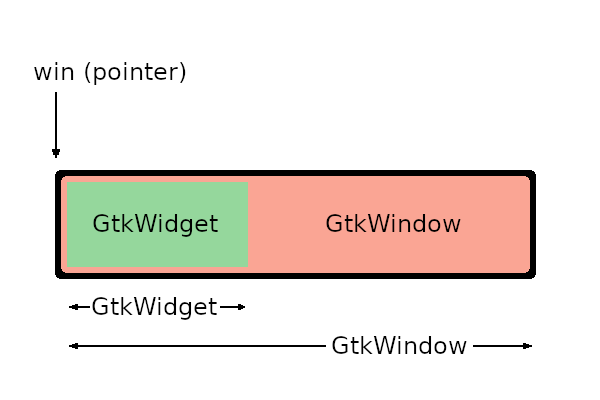
\includegraphics[width=9cm,height=6cm]{../image/window_widget.png}
\caption{GtkWindow and GtkWidget}
\end{figure}

The function \passthrough{\lstinline!gtk\_window\_new!} is defined as
follows.

\begin{lstlisting}[language=C]
GtkWidget *
gtk_window_new (void);
\end{lstlisting}

By this definition, it returns a pointer to GtkWidget, not GtkWindow. It
actually creates a new GtkWindow instance (not GtkWidget) but returns a
pointer to GtkWidget. However,the pointer points the GtkWidget and at
the same time it also points GtkWindow that contains GtkWidget in it.

If you want to use \passthrough{\lstinline!win!} as a pointer to a
GtkWindow type instance, you need to cast it.

\begin{lstlisting}[language=C]
(GtkWindow *) win
\end{lstlisting}

It works, but isn't usually used. Instead,
\passthrough{\lstinline!GTK\_WINDOW!} macro is used.

\begin{lstlisting}[language=C]
GTK_WINDOW (win)
\end{lstlisting}

The macro is recommended because it does not only cast the pointer but
it also checks the type.

\paragraph{Connect it to the
GtkApplication.}\label{connect-it-to-the-gtkapplication.}

The function \passthrough{\lstinline!gtk\_window\_set\_application!} is
used to connect GtkWindow to GtkApplication.

\begin{lstlisting}[language=C]
gtk_window_set_application (GTK_WINDOW (win), GTK_APPLICATION (app));
\end{lstlisting}

You need to cast \passthrough{\lstinline!win!} to GtkWindow and
\passthrough{\lstinline!app!} to GtkApplication with
\passthrough{\lstinline!GTK\_WINDOW!} and
\passthrough{\lstinline!GTK\_APPLICATION!} macro.

GtkApplication continues to run until the related window is destroyed.
If you didn't connect GtkWindow and GtkApplication, GtkApplication
destroys itself immediately. Because no window is connected to
GtkApplication, GtkApplication doesn't need to wait anything. As it
destroys itself, the GtkWindow is also destroyed.

\paragraph{Show the window.}\label{show-the-window.}

The function \passthrough{\lstinline!gtk\_window\_present!} presents the
window to a user (shows it to the user).

GTK 4 changes the default widget visibility to on, so every widget
doesn't need to change it to on. But, there's an exception. Top level
window (this term will be explained later) isn't visible when it is
created. So you need to use the function above to show the window.

You can use
\passthrough{\lstinline!gtk\_widget\_set\_visible (win, true)!} instead
of \passthrough{\lstinline!gtk\_window\_present!}. But the behavior of
these two is different. Suppose there are two windows win1 and win2 on
the screen and win1 is behind win2. Both windows are visible. The
function
\passthrough{\lstinline!gtk\_widget\_set\_visible (win1, true)!} does
nothing because win1 is already visible. So, win1 is still behind win2.
The other function \passthrough{\lstinline!gtk\_window\_present (win1)!}
moves win1 to the top of the stack of the windows. Therefore, if you
want to present the window, you should use
\passthrough{\lstinline!gtk\_window\_present!}.

Two functions \passthrough{\lstinline!gtk\_widget\_show!} and
\passthrough{\lstinline!gtk\_widget\_hide!} is deprecated since GTK
4.10. You should use \passthrough{\lstinline!gtk\_widget\_set\_visible!}
instead.

Save the program as \passthrough{\lstinline!pr3.c!}, then compile and
run it.

\begin{lstlisting}
$ comp pr3
$ ./a.out
\end{lstlisting}

A small window appears.

\begin{figure}
\centering
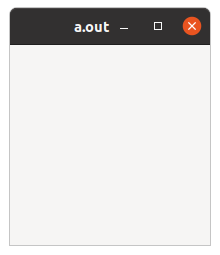
\includegraphics[width=3.3cm,height=3.825cm]{../image/screenshot_pr3.png}
\caption{Screenshot of the window}
\end{figure}

Click on the close button then the window disappears and the program
finishes.

\subsubsection{GtkApplicationWindow}\label{gtkapplicationwindow}

GtkApplicationWindow is a child object of GtkWindow. It has some extra
feature for better integration with GtkApplication. It is recommended to
use it as the top-level window of the application instead of GtkWindow.

Now rewrite the program and use GtkApplicationWindow.

\begin{lstlisting}[language=C, numbers=left]
static void
app_activate (GApplication *app, gpointer user_data) {
  GtkWidget *win;

  win = gtk_application_window_new (GTK_APPLICATION (app));
  gtk_window_set_title (GTK_WINDOW (win), "pr4");
  gtk_window_set_default_size (GTK_WINDOW (win), 400, 300);
  gtk_window_present (GTK_WINDOW (win));
}
\end{lstlisting}

When you create GtkApplicationWindow, you need to give GtkApplication
instance as an argument. Then it automatically connect these two
instances. So you don't need to call
\passthrough{\lstinline!gtk\_window\_set\_application!} any more.

The program sets the title and the default size of the window. Compile
it and run \passthrough{\lstinline!a.out!}, then you will see a bigger
window with the title ``pr4''.

\begin{figure}
\centering
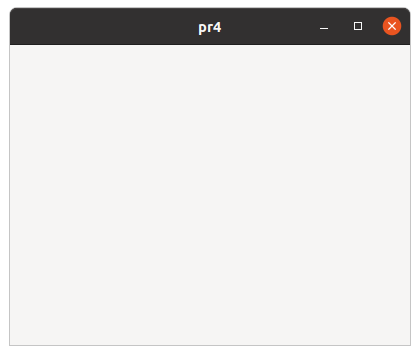
\includegraphics[width=6.3cm,height=5.325cm]{../image/screenshot_pr4.png}
\caption{Screenshot of the window}
\end{figure}

  \section{Widgets (1)}\label{widgets-1}

\subsection{GtkLabel, GtkButton and
GtkBox}\label{gtklabel-gtkbutton-and-gtkbox}

\subsubsection{GtkLabel}\label{gtklabel}

We made a window and showed it on the screen in the previous section.
Now we go on to the next topic: widgets. The simplest widget is
GtkLabel. It is a widget with text in it.

\begin{lstlisting}[language=C, numbers=left]
#include <gtk/gtk.h>

static void
app_activate (GApplication *app) {
  GtkWidget *win;
  GtkWidget *lab;

  win = gtk_application_window_new (GTK_APPLICATION (app));
  gtk_window_set_title (GTK_WINDOW (win), "lb1");
  gtk_window_set_default_size (GTK_WINDOW (win), 400, 300);

  lab = gtk_label_new ("Hello.");
  gtk_window_set_child (GTK_WINDOW (win), lab);

  gtk_window_present (GTK_WINDOW (win));
}

int
main (int argc, char **argv) {
  GtkApplication *app;
  int stat;

  app = gtk_application_new ("com.github.ToshioCP.lb1", G_APPLICATION_DEFAULT_FLAGS);
  g_signal_connect (app, "activate", G_CALLBACK (app_activate), NULL);
  stat =g_application_run (G_APPLICATION (app), argc, argv);
  g_object_unref (app);
  return stat;
}
\end{lstlisting}

Save this program to a file \passthrough{\lstinline!lb1.c!}. (You can
use \passthrough{\lstinline!src/misc/lb1.c!} if you've downloaded this
repository.) Then compile and run it.

\begin{lstlisting}
$ comp lb1
$ ./a.out
\end{lstlisting}

A window with a message ``Hello.'' appears.

\begin{figure}
\centering
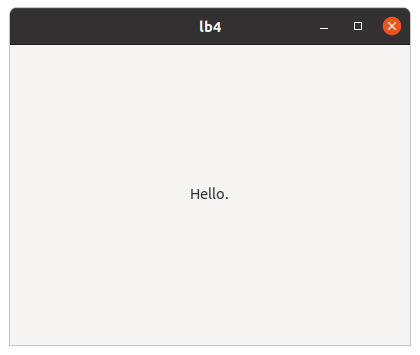
\includegraphics[width=6.3cm,height=5.325cm]{../image/screenshot_lb1.png}
\caption{Screenshot of the label}
\end{figure}

There are only a few changes between \passthrough{\lstinline!pr4.c!} and
\passthrough{\lstinline!lb1.c!}. A program
\passthrough{\lstinline!diff!} is useful to know the difference.

\begin{lstlisting}
$ cd misc; diff pr4.c lb1.c
4c4
< app_activate (GApplication *app, gpointer user_data) {
---
> app_activate (GApplication *app) {
5a6
>   GtkWidget *lab;
8c9
<   gtk_window_set_title (GTK_WINDOW (win), "pr4");
---
>   gtk_window_set_title (GTK_WINDOW (win), "lb1");
9a11,14
> 
>   lab = gtk_label_new ("Hello.");
>   gtk_window_set_child (GTK_WINDOW (win), lab);
> 
18c23
<   app = gtk_application_new ("com.github.ToshioCP.pr4", G_APPLICATION_DEFAULT_FLAGS);
---
>   app = gtk_application_new ("com.github.ToshioCP.lb1", G_APPLICATION_DEFAULT_FLAGS);
\end{lstlisting}

This tells us:

\begin{itemize}
\tightlist
\item
  A signal handler \passthrough{\lstinline!app\_activate!} doesn't have
  \passthrough{\lstinline!user\_data!} parameter. If the fourth argument
  of \passthrough{\lstinline!g\_signal\_connect!} is NULL, you can leave
  out \passthrough{\lstinline!user\_data!}.
\item
  The definition of a new variable \passthrough{\lstinline!lab!} is
  added.
\item
  The title of the window is changed.
\item
  A label is created and connected to the window as a child.
\end{itemize}

The function
\passthrough{\lstinline!gtk\_window\_set\_child (GTK\_WINDOW (win), lab)!}
makes the label \passthrough{\lstinline!lab!} a child widget of the
window \passthrough{\lstinline!win!}. Be careful. A child widget is
different from a child object. Objects have parent-child relationships
and widgets also have parent-child relationships. But these two
relationships are totally different. Don't be confused. In the program
\passthrough{\lstinline!lb1.c!}, \passthrough{\lstinline!lab!} is a
child widget of \passthrough{\lstinline!win!}. Child widgets are always
located in their parent widget on the screen. See how the window has
appeared on the screen. The application window includes the label.

The window \passthrough{\lstinline!win!} doesn't have any parents. We
call such a window top-level window. An application can have more than
one top-level windows.

\subsubsection{GtkButton}\label{gtkbutton}

The next widget is GtkButton. It displays a button on the screen with a
label or icon on it. In this subsection, we will make a button with a
label. When the button is clicked, it emits a ``clicked'' signal. The
following program shows how to catch the signal and do something.

\begin{lstlisting}[language=C, numbers=left]
#include <gtk/gtk.h>

static void
click_cb (GtkButton *btn) {
  g_print ("Clicked.\n");
}

static void
app_activate (GApplication *app) {
  GtkWidget *win;
  GtkWidget *btn;

  win = gtk_application_window_new (GTK_APPLICATION (app));
  gtk_window_set_title (GTK_WINDOW (win), "lb2");
  gtk_window_set_default_size (GTK_WINDOW (win), 400, 300);

  btn = gtk_button_new_with_label ("Click me");
  gtk_window_set_child (GTK_WINDOW (win), btn);
  g_signal_connect (btn, "clicked", G_CALLBACK (click_cb), NULL);

  gtk_window_present (GTK_WINDOW (win));
}

int
main (int argc, char **argv) {
  GtkApplication *app;
  int stat;

  app = gtk_application_new ("com.github.ToshioCP.lb2", G_APPLICATION_DEFAULT_FLAGS);
  g_signal_connect (app, "activate", G_CALLBACK (app_activate), NULL);
  stat =g_application_run (G_APPLICATION (app), argc, argv);
  g_object_unref (app);
  return stat;
}
\end{lstlisting}

Look at the line 17 to 19. First, it creates a GtkButton instance
\passthrough{\lstinline!btn!} with a label ``Click me''. Then, adds the
button to the window \passthrough{\lstinline!win!} as a child. Finally,
connects the ``clicked'' signal of the button to the handler
\passthrough{\lstinline!click\_cb!}. So, if
\passthrough{\lstinline!btn!} is clicked, the function
\passthrough{\lstinline!click\_cb!} is invoked. The suffix ``cb'' means
``call back''.

Name the program \passthrough{\lstinline!lb2.c!} and save it. Now
compile and run it.

\begin{figure}
\centering
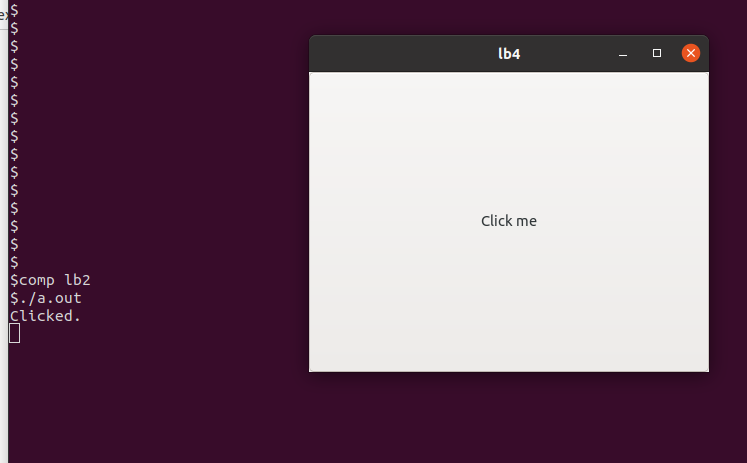
\includegraphics[width=11.205cm,height=6.945cm]{../image/screenshot_lb2.png}
\caption{Screenshot of the label}
\end{figure}

A window with the button appears. Click the button (it is a large
button, you can click everywhere in the window), then a string
``Clicked.'' appears on the terminal. It shows the handler was invoked
by clicking the button.

It's good that we've made sure that the clicked signal was caught and
the handler was invoked by using \passthrough{\lstinline!g\_print!}.
However, using \passthrough{\lstinline!g\_print!} is out of harmony with
GTK, which is a GUI library. So, we will change the handler. The
following code is extracted from \passthrough{\lstinline!lb3.c!}.

\begin{lstlisting}[language=C, numbers=left]
static void
click_cb (GtkButton *btn, GtkWindow *win) {
  gtk_window_destroy (win);
}

static void
app_activate (GApplication *app) {
  GtkWidget *win;
  GtkWidget *btn;

  win = gtk_application_window_new (GTK_APPLICATION (app));
  gtk_window_set_title (GTK_WINDOW (win), "lb3");
  gtk_window_set_default_size (GTK_WINDOW (win), 400, 300);

  btn = gtk_button_new_with_label ("Close");
  gtk_window_set_child (GTK_WINDOW (win), btn);
  g_signal_connect (btn, "clicked", G_CALLBACK (click_cb), win);

  gtk_window_present (GTK_WINDOW (win));
}
\end{lstlisting}

And the difference between \passthrough{\lstinline!lb2.c!} and
\passthrough{\lstinline!lb3.c!} is as follows.

\begin{lstlisting}
$ cd misc; diff lb2.c lb3.c
4,5c4,5
< click_cb (GtkButton *btn) {
<   g_print ("Clicked.\n");
---
> click_cb (GtkButton *btn, GtkWindow *win) {
>   gtk_window_destroy (win);
14c14
<   gtk_window_set_title (GTK_WINDOW (win), "lb2");
---
>   gtk_window_set_title (GTK_WINDOW (win), "lb3");
17c17
<   btn = gtk_button_new_with_label ("Click me");
---
>   btn = gtk_button_new_with_label ("Close");
19c19
<   g_signal_connect (btn, "clicked", G_CALLBACK (click_cb), NULL);
---
>   g_signal_connect (btn, "clicked", G_CALLBACK (click_cb), win);
29c29
<   app = gtk_application_new ("com.github.ToshioCP.lb2", G_APPLICATION_DEFAULT_FLAGS);
---
>   app = gtk_application_new ("com.github.ToshioCP.lb3", G_APPLICATION_DEFAULT_FLAGS);
35d34
< 
\end{lstlisting}

The changes are:

\begin{itemize}
\tightlist
\item
  The function \passthrough{\lstinline!g\_print!} in
  \passthrough{\lstinline!lb2.c!} was deleted and two lines are
  inserted.

  \begin{itemize}
  \tightlist
  \item
    \passthrough{\lstinline!click\_cb!} has the second parameter, which
    comes from the fourth argument of the
    \passthrough{\lstinline!g\_signal\_connect!} at line 17. One thing
    to be careful is the types are different between the second
    parameter of \passthrough{\lstinline!click\_cb!} and the fourth
    argument of \passthrough{\lstinline!g\_signal\_connect!}. The former
    is \passthrough{\lstinline!GtkWindow *!} and the latter is
    \passthrough{\lstinline!GtkWidget *!}. The compiler doesn't complain
    because \passthrough{\lstinline!g\_signal\_connect!} uses gpointer
    (general type of pointer). In this program the instance pointed by
    \passthrough{\lstinline!win!} is a GtkApplicationWindow object. It
    is a descendant of GtkWindow and GtkWidget class, so both
    \passthrough{\lstinline!GtkWindow *!} and
    \passthrough{\lstinline!GtkWidget *!} are correct types of the
    instance.
  \item
    \passthrough{\lstinline!gtk\_destroy (win)!} destroys the top-level
    window. Then the application quits.
  \end{itemize}
\item
  The label of \passthrough{\lstinline!btn!} is changed from ``Click
  me'' to ``Close''.
\item
  The fourth argument of \passthrough{\lstinline!g\_signal\_connect!} is
  changed from \passthrough{\lstinline!NULL!} to
  \passthrough{\lstinline!win!}.
\end{itemize}

The most important change is the fourth argument of the
\passthrough{\lstinline!g\_signal\_connect!}. This argument is described
as ``data to pass to the handler'' in the definition of
\href{https://docs.gtk.org/gobject/func.signal_connect.html}{\passthrough{\lstinline!g\_signal\_connect!}}.

\subsubsection{GtkBox}\label{gtkbox}

GtkWindow and GtkApplicationWindow can have only one child. If you want
to add two or more widgets in a window, you need a container widget.
GtkBox is one of the containers. It arranges two or more child widgets
into a single row or column. The following procedure shows the way to
add two buttons in a window.

\begin{itemize}
\tightlist
\item
  Create a GtkApplicationWindow instance.
\item
  Create a GtkBox instance and add it to the GtkApplicationWindow as a
  child.
\item
  Create a GtkButton instance and append it to the GtkBox.
\item
  Create another GtkButton instance and append it to the GtkBox.
\end{itemize}

After this, the Widgets are connected as the following diagram.

\begin{figure}
\centering
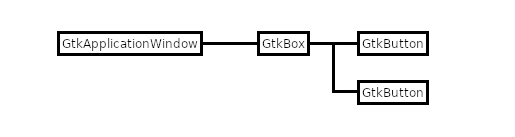
\includegraphics[width=7.725cm,height=2.055cm]{../image/box.png}
\caption{Parent-child relationship}
\end{figure}

The program \passthrough{\lstinline!lb4.c!} is as follows.

\begin{lstlisting}[language=C, numbers=left]
#include <gtk/gtk.h>

static void
click1_cb (GtkButton *btn) {
  const char *s;

  s = gtk_button_get_label (btn);
  if (g_strcmp0 (s, "Hello.") == 0)
    gtk_button_set_label (btn, "Good-bye.");
  else
    gtk_button_set_label (btn, "Hello.");
}

static void
click2_cb (GtkButton *btn, GtkWindow *win) {
  gtk_window_destroy (win);
}

static void
app_activate (GApplication *app) {
  GtkWidget *win;
  GtkWidget *box;
  GtkWidget *btn1;
  GtkWidget *btn2;

  win = gtk_application_window_new (GTK_APPLICATION (app));
  gtk_window_set_title (GTK_WINDOW (win), "lb4");
  gtk_window_set_default_size (GTK_WINDOW (win), 400, 300);

  box = gtk_box_new (GTK_ORIENTATION_VERTICAL, 5);
  gtk_box_set_homogeneous (GTK_BOX (box), TRUE);
  gtk_window_set_child (GTK_WINDOW (win), box);

  btn1 = gtk_button_new_with_label ("Hello.");
  g_signal_connect (btn1, "clicked", G_CALLBACK (click1_cb), NULL);

  btn2 = gtk_button_new_with_label ("Close");
  g_signal_connect (btn2, "clicked", G_CALLBACK (click2_cb), win);

  gtk_box_append (GTK_BOX (box), btn1);
  gtk_box_append (GTK_BOX (box), btn2);

  gtk_window_present (GTK_WINDOW (win));
}

int
main (int argc, char **argv) {
  GtkApplication *app;
  int stat;

  app = gtk_application_new ("com.github.ToshioCP.lb4", G_APPLICATION_DEFAULT_FLAGS);
  g_signal_connect (app, "activate", G_CALLBACK (app_activate), NULL);
  stat =g_application_run (G_APPLICATION (app), argc, argv);
  g_object_unref (app);
  return stat;
}
\end{lstlisting}

Look at the function \passthrough{\lstinline!app\_activate!}.

After the creation of a GtkApplicationWindow instance, a GtkBox instance
is created.

\begin{lstlisting}[language=C]
box = gtk_box_new(GTK_ORIENTATION_VERTICAL, 5);
gtk_box_set_homogeneous (GTK_BOX (box), TRUE);
\end{lstlisting}

The first argument arranges the children of the box vertically. The
orientation constants are defined like this:

\begin{itemize}
\tightlist
\item
  GTK\_ORIENTATION\_VERTICAL: the children widgets are arranged
  vertically
\item
  GTK\_ORIENTATION\_HORIZONTAL: the children widgets are arranged
  horizontally
\end{itemize}

The second argument is the size of the space between the children. The
unit of the length is pixel.

The next function fills the box with the children, giving them the same
space.

After that, two buttons \passthrough{\lstinline!btn1!} and
\passthrough{\lstinline!btn2!} are created and the signal handlers are
set. Then, these two buttons are appended to the box.

\begin{lstlisting}[language=C, numbers=left]
static void
click1_cb (GtkButton *btn) {
  const char *s;

  s = gtk_button_get_label (btn);
  if (g_strcmp0 (s, "Hello.") == 0)
    gtk_button_set_label (btn, "Good-bye.");
  else
    gtk_button_set_label (btn, "Hello.");
}
\end{lstlisting}

The function \passthrough{\lstinline!gtk\_button\_get\_label!} returns a
text from the label. The string is owned by the button and you can't
modify or free it. The \passthrough{\lstinline!const!} qualifier is
necessary for the string \passthrough{\lstinline!s!}. If you change the
string, your compiler will give you a waring.

You always need to be careful with the const qualifier when you see the
GTK 4 API reference.

\begin{figure}
\centering
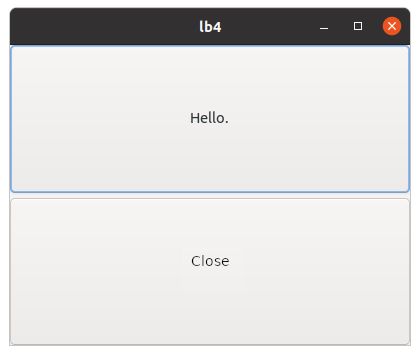
\includegraphics[width=6.3cm,height=5.325cm]{../image/screenshot_lb4.png}
\caption{Screenshot of the box}
\end{figure}

The handler corresponding to \passthrough{\lstinline!btn1!} toggles its
label. The handler corresponding to \passthrough{\lstinline!btn2!}
destroys the top-level window and the application quits.

  \section{Widgets (2)}\label{widgets-2}

\subsection{GtkTextView, GtkTextBuffer and
GtkScrolledWindow}\label{gtktextview-gtktextbuffer-and-gtkscrolledwindow}

\subsubsection{GtkTextView and
GtkTextBuffer}\label{gtktextview-and-gtktextbuffer}

GtkTextView is a widget for multi-line text editing. GtkTextBuffer is a
text buffer which is connected to GtkTextView. See the sample program
\passthrough{\lstinline!tfv1.c!} below.

\begin{lstlisting}[language=C, numbers=left]
#include <gtk/gtk.h>

static void
app_activate (GApplication *app) {
  GtkWidget *win;
  GtkWidget *tv;
  GtkTextBuffer *tb;
  gchar *text;

  text =
      "Once upon a time, there was an old man who was called Taketori-no-Okina. "
      "It is a japanese word that means a man whose work is making bamboo baskets.\n"
      "One day, he went into a hill and found a shining bamboo. "
      "\"What a mysterious bamboo it is!,\" he said. "
      "He cut it, then there was a small cute baby girl in it. "
      "The girl was shining faintly. "
      "He thought this baby girl is a gift from Heaven and took her home.\n"
      "His wife was surprized at his story. "
      "They were very happy because they had no children. "
      ;
  win = gtk_application_window_new (GTK_APPLICATION (app));
  gtk_window_set_title (GTK_WINDOW (win), "Taketori");
  gtk_window_set_default_size (GTK_WINDOW (win), 400, 300);

  tv = gtk_text_view_new ();
  tb = gtk_text_view_get_buffer (GTK_TEXT_VIEW (tv));
  gtk_text_buffer_set_text (tb, text, -1);
  gtk_text_view_set_wrap_mode (GTK_TEXT_VIEW (tv), GTK_WRAP_WORD_CHAR);

  gtk_window_set_child (GTK_WINDOW (win), tv);

  gtk_window_present (GTK_WINDOW (win));
}

int
main (int argc, char **argv) {
  GtkApplication *app;
  int stat;

  app = gtk_application_new ("com.github.ToshioCP.tfv1", G_APPLICATION_DEFAULT_FLAGS);
  g_signal_connect (app, "activate", G_CALLBACK (app_activate), NULL);
  stat = g_application_run (G_APPLICATION (app), argc, argv);
  g_object_unref (app);
  return stat;
}
\end{lstlisting}

Look at line 25. A GtkTextView instance is created and its pointer is
assigned to \passthrough{\lstinline!tv!}. When the GtkTextView instance
is created, a GtkTextBuffer instance is also created and connected to
the GtkTextView automatically. ``GtkTextBuffer instance'' will be
referred to simply as ``GtkTextBuffer'' or ``buffer''. In the next line,
the pointer to the buffer is assigned to \passthrough{\lstinline!tb!}.
Then, the text from line 10 to 20 is assigned to the buffer. If the
third argument of \passthrough{\lstinline!gtk\_text\_buffer\_set\_text!}
is a positive integer, it is the length of the text. It it is -1, the
string terminates with NULL.

GtkTextView has a wrap mode. When it is set to
\passthrough{\lstinline!GTK\_WRAP\_WORD\_CHAR!}, text wraps in between
words, or if that is not enough, also between graphemes.

Wrap mode is written in
\href{https://docs.gtk.org/gtk4/enum.WrapMode.html}{Gtk\_WrapMode} in
the GTK 4 API document.

In line 30, \passthrough{\lstinline!tv!} is added to
\passthrough{\lstinline!win!} as a child.

Now compile and run it. If you've downloaded this repository, its
pathname is \passthrough{\lstinline!src/tfv/tfv1.c!}.

\begin{lstlisting}
$ cd src/tfv
$ comp tfv1
$ ./a.out
\end{lstlisting}

\begin{figure}
\centering
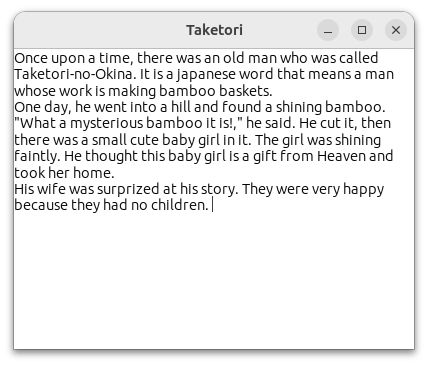
\includegraphics[width=6.3cm,height=5.325cm]{../image/screenshot_tfv1.png}
\caption{GtkTextView}
\end{figure}

There's an I-beam pointer in the window. You can add or delete any
characters on the GtkTextView, and your changes are kept in the
GtkTextBuffer. If you add more characters beyond the limit of the
window, the height increases and the window extends. If the height gets
bigger than the height of the screen, you won't be able to control the
size of the window or change it back to the original size. This is a
problem, that is to say a bug. This can be solved by adding a
GtkScrolledWindow between the GtkApplicationWindow and GtkTextView.

\subsubsection{GtkScrolledWindow}\label{gtkscrolledwindow}

What we need to do is:

\begin{itemize}
\tightlist
\item
  Create a GtkScrolledWindow and insert it as a child of the
  GtkApplicationWindow
\item
  Insert the GtkTextView widget to the GtkScrolledWindow as a child.
\end{itemize}

Modify \passthrough{\lstinline!tfv1.c!} and save it as
\passthrough{\lstinline!tfv2.c!}. There is only a few difference between
these two files.

\begin{lstlisting}
$ cd tfv; diff tfv1.c tfv2.c
5a6
>   GtkWidget *scr;
24a26,28
>   scr = gtk_scrolled_window_new ();
>   gtk_window_set_child (GTK_WINDOW (win), scr);
> 
30c34
<   gtk_window_set_child (GTK_WINDOW (win), tv);
---
>   gtk_scrolled_window_set_child (GTK_SCROLLED_WINDOW (scr), tv);
40c44
<   app = gtk_application_new ("com.github.ToshioCP.tfv1", G_APPLICATION_DEFAULT_FLAGS);
---
>   app = gtk_application_new ("com.github.ToshioCP.tfv2", G_APPLICATION_DEFAULT_FLAGS);
\end{lstlisting}

The whole code of \passthrough{\lstinline!tfv2.c!} is as follows.

\begin{lstlisting}[language=C, numbers=left]
#include <gtk/gtk.h>

static void
app_activate (GApplication *app) {
  GtkWidget *win;
  GtkWidget *scr;
  GtkWidget *tv;
  GtkTextBuffer *tb;
  gchar *text;

  text =
      "Once upon a time, there was an old man who was called Taketori-no-Okina. "
      "It is a japanese word that means a man whose work is making bamboo baskets.\n"
      "One day, he went into a hill and found a shining bamboo. "
      "\"What a mysterious bamboo it is!,\" he said. "
      "He cut it, then there was a small cute baby girl in it. "
      "The girl was shining faintly. "
      "He thought this baby girl is a gift from Heaven and took her home.\n"
      "His wife was surprized at his story. "
      "They were very happy because they had no children. "
      ;
  win = gtk_application_window_new (GTK_APPLICATION (app));
  gtk_window_set_title (GTK_WINDOW (win), "Taketori");
  gtk_window_set_default_size (GTK_WINDOW (win), 400, 300);

  scr = gtk_scrolled_window_new ();
  gtk_window_set_child (GTK_WINDOW (win), scr);

  tv = gtk_text_view_new ();
  tb = gtk_text_view_get_buffer (GTK_TEXT_VIEW (tv));
  gtk_text_buffer_set_text (tb, text, -1);
  gtk_text_view_set_wrap_mode (GTK_TEXT_VIEW (tv), GTK_WRAP_WORD_CHAR);

  gtk_scrolled_window_set_child (GTK_SCROLLED_WINDOW (scr), tv);

  gtk_window_present (GTK_WINDOW (win));
}

int
main (int argc, char **argv) {
  GtkApplication *app;
  int stat;

  app = gtk_application_new ("com.github.ToshioCP.tfv2", G_APPLICATION_DEFAULT_FLAGS);
  g_signal_connect (app, "activate", G_CALLBACK (app_activate), NULL);
  stat = g_application_run (G_APPLICATION (app), argc, argv);
  g_object_unref (app);
  return stat;
}
\end{lstlisting}

Compile and run it.

Now, the window doesn't extend even if you type a lot of characters, it
just scrolls.

  \section{Strings and memory
management}\label{strings-and-memory-management}

GtkTextView and GtkTextBuffer have functions that have string parameters
or return a string. The knowledge of strings and memory management is
useful to understand how to use these functions.

\subsection{String and memory}\label{string-and-memory}

A String is an array of characters that is terminated with
`\textbackslash0'. String is not a C type such as char, int, float or
double, but a character array. It behaves like a string in other
languages. So, the pointer is often called `a string'.

The following is a sample program.

\begin{lstlisting}[language=C]
char a[10], *b;

a[0] = 'H';
a[1] = 'e';
a[2] = 'l';
a[3] = 'l';
a[4] = 'o';
a[5] = '\0';

b = a;
/* *b is 'H' */
/* *(++b) is 'e' */
\end{lstlisting}

An array \passthrough{\lstinline!a!} is defined as a
\passthrough{\lstinline!char!} type array and its size is ten. The first
five elements are `H', `e', `l', `l', `o'. They are character codes. For
example, `H' is the same as 0x48 or 72. The sixth element is
`\textbackslash0', which is the same as zero, and indicates that the
sequence of the data ends there. The array represents the string
``Hello''.

The size of the array is 10, so four bytes aren't used. But it's OK.
They are just ignored. (If the variable \passthrough{\lstinline!a!} is
defined out of functions or its class is static, the four bytes are
assigned with zero. Otherwise, that is to say, the class is auto or
register, they are undefined.)

The variable \passthrough{\lstinline!b!} is a pointer to a character. It
is assigned with \passthrough{\lstinline!a!}, so
\passthrough{\lstinline!b!} points the first element of
\passthrough{\lstinline!a!} (character `H'). The array
\passthrough{\lstinline!a!} is immutable. So
\passthrough{\lstinline!a=a+1!} causes syntax error.

On the other hand, \passthrough{\lstinline!b!} is a pointer type
variable, which is mutable. So, \passthrough{\lstinline!++b!}, which
increases \passthrough{\lstinline!b!} by one, is allowed.

If a pointer is NULL, it points nothing. So, the pointer is not a
string. It is different from empty string. Empty string is a pointer
points `\textbackslash0'.

There are four cases:

\begin{itemize}
\tightlist
\item
  The string is read only
\item
  The string is in static memory area
\item
  The string is in stack
\item
  The string is in memory allocated from the heap area
\end{itemize}

\subsection{Read only string}\label{read-only-string}

A string literal is surrounded by double quotes like this:

\begin{lstlisting}[language=C]
char *s;
s = "Hello"
\end{lstlisting}

``Hello'' is a string literal, and is read only. So, the following
program is illegal.

\begin{lstlisting}[language=C]
*(s+1) = 'a';
\end{lstlisting}

The result is undefined. Probably a bad thing will happen, for example,
a segmentation fault.

NOTE: The memory of the literal string is allocated when the program is
compiled. It is possible to see the literal strings with
\passthrough{\lstinline!strings!} command.

\begin{lstlisting}
$ strings src/tvf/a.out
/lib64/ld-linux-x86-64.so.2
cN<5
... ... ...
... ... ...
Once upon a time, there was an old man who was called Taketori-no-Okina. It is a japanese word that means a man whose work is making bamboo baskets.
One day, he went into a hill and found a shining bamboo. "What a mysterious bamboo it is!," he said. He cut it, then there was a small cute baby girl in it. The girl was shining faintly. He thought this baby girl is a gift from Heaven and took her home.
His wife was surprized at his story. They were very happy because they had no children. 
... ... ...
... ... ...
\end{lstlisting}

It tells us that literal strings are embedded in program binary codes.

\subsection{Strings defined as arrays}\label{strings-defined-as-arrays}

If a string is defined as an array, it's stored in static memory area or
stack. It depends on the class of the array. If the array's class is
\passthrough{\lstinline!static!}, then it's placed in static memory
area. The allocated memory lives for the life of the program. This area
is writable.

If the array's class is \passthrough{\lstinline!auto!}, it's placed in
stack. If the array is defined inside a function, its default class is
\passthrough{\lstinline!auto!}. The stack area will disappear when the
function returns to the caller. Arrays defined on the stack are
writable.

\begin{lstlisting}[language=C]
static char a[] = {'H', 'e', 'l', 'l', 'o', '\0'};

void
print_strings (void) {
  char b[] = "Hello";

  a[1] = 'a'; /* Because the array is static, it's writable. */
  b[1] = 'a'; /* Because the array is auto, it's writable. */

  printf ("%s\n", a); /* Hallo */
  printf ("%s\n", b); /* Hallo */
}
\end{lstlisting}

The array \passthrough{\lstinline!a!} is defined out of functions. It is
placed in the static memory area even if the
\passthrough{\lstinline!static!} class is left out. The compiler
calculates the number of the elements (six) and allocates six bytes in
the static memory area. Then, it copies ``Hello'' literal string data to
the memory.

The array \passthrough{\lstinline!b!} is defined inside the function, so
its class is \passthrough{\lstinline!auto!}. The compiler calculates the
number of the elements in the string literal. It is six because it has
`\textbackslash0' terminator. The compiler allocates six bytes in the
stack and copies ``Hello'' litaral string to the stack memory.

Both \passthrough{\lstinline!a!} and \passthrough{\lstinline!b!} are
writable.

The memory is allocated and freed by the program automatically so you
don't need to allocate or free. The array \passthrough{\lstinline!a!} is
alive during the program's life time. The array
\passthrough{\lstinline!b!} is alive when the function is called until
the function returns to the caller.

\subsection{Strings in the heap area}\label{strings-in-the-heap-area}

You can get, use and release memory from the heap area. The standard C
library provides \passthrough{\lstinline!malloc!} to get memory and
\passthrough{\lstinline!free!} to put back memory. GLib provides the
functions \passthrough{\lstinline!g\_new!} and
\passthrough{\lstinline!g\_free!}. They are similar to
\passthrough{\lstinline!malloc!} and \passthrough{\lstinline!free!}.

\begin{lstlisting}[language=C]
g_new (struct_type, n_struct)
\end{lstlisting}

\passthrough{\lstinline!g\_new!} is a macro to allocate memory for an
array.

\begin{itemize}
\tightlist
\item
  \passthrough{\lstinline!struct\_type!} is the type of the element of
  the array.
\item
  \passthrough{\lstinline!n\_struct!} is the size of the array.
\item
  The return value is a pointer to the array. Its type is a pointer to
  \passthrough{\lstinline!struct\_type!}.
\end{itemize}

For example,

\begin{lstlisting}[language=C]
char *s;
s = g_new (char, 10);
/* s points an array of char. The size of the array is 10. */

struct tuple {int x, y;} *t;
t = g_new (struct tuple, 5);
/* t points an array of struct tuple. */
/* The size of the array is 5. */
\end{lstlisting}

\passthrough{\lstinline!g\_free!} frees memory.

\begin{lstlisting}[language=C]
void
g_free (gpointer mem);
\end{lstlisting}

If \passthrough{\lstinline!mem!} is NULL,
\passthrough{\lstinline!g\_free!} does nothing.
\passthrough{\lstinline!gpointer!} is a type of general pointer. It is
the same as \passthrough{\lstinline!void *!}. This pointer can be casted
to any pointer type. Conversely, any pointer type can be casted to
\passthrough{\lstinline!gpointer!}.

\begin{lstlisting}[language=C]
g_free (s);
/* Frees the memory allocated to s. */

g_free (t);
/* Frees the memory allocated to t. */
\end{lstlisting}

If the argument doesn't point allocated memory it will cause an error,
specifically, a segmentation fault.

Some GLib functions allocate memory. For example,
\passthrough{\lstinline!g\_strdup!} allocates memory and copies a string
given as an argument.

\begin{lstlisting}[language=C]
char *s;
s = g_strdup ("Hello");
g_free (s);
\end{lstlisting}

The string literal ``Hello'' has 6 bytes because the string has
`\textbackslash0' at the end. \passthrough{\lstinline!g\_strdup!} gets 6
bytes from the heap area and copies the string to the memory.
\passthrough{\lstinline!s!} is assigned the start address of the memory.
\passthrough{\lstinline!g\_free!} returns the memory to the heap area.

\passthrough{\lstinline!g\_strdup!} is described in
\href{https://docs.gtk.org/glib/func.strdup.html}{GLib API Reference}.
The following is extracted from the reference.

\begin{quote}
The returned string should be freed with
\passthrough{\lstinline!g\_free()!} when no longer needed.
\end{quote}

If you forget to free the allocated memory it will remain until the
program ends. Repeated allocation and no freeing cause memory leak. It
is a bug and may bring a serious problem.

\subsection{const qualifier}\label{const-qualifier}

A \passthrough{\lstinline!const!} qualified variable can be assigned to
initialize it. Once it is initialized, it is never allowed to change or
free.

\begin{lstlisting}[language=C]
const int x = 10; /* initialization is OK. */

x = 20; /* This is illegal because x is qualified with const */
\end{lstlisting}

If a function returns \passthrough{\lstinline!const char*!} type, the
string can't be changed or freed. If a function has a
\passthrough{\lstinline!const char *!} type parameter, it ensures that
the parameter is not changed in the function.

\begin{lstlisting}[language=C]
// You never change or free the returned string.
const char*
gtk_label_get_text (
  GtkLabel* self
)

// Str keeps itself during the function runs
void
gtk_label_set_text (
  GtkLabel* self,
  const char* str
)
\end{lstlisting}

  \section{Widgets (3)}\label{widgets-3}

\subsection{Open signal}\label{open-signal}

\subsubsection{G\_APPLICATION\_HANDLES\_OPEN
flag}\label{g_application_handles_open-flag}

We made a very simple editor in the previous section with GtkTextView,
GtkTextBuffer and GtkScrolledWindow. We will add file-read ability to
the program and improve it to a file viewer.

The easiest way to give a filename is to use a command line argument.

\begin{lstlisting}
$ ./a.out filename
\end{lstlisting}

The program will open the file and insert its contents into the
GtkTextBuffer.

To do this, we need to know how GtkApplication (or GApplication)
recognizes arguments. This is described in the
\href{https://docs.gtk.org/gio/class.Application.html}{GIO API Reference
-- Application}.

When GtkApplication is created, a flag (GApplicationFlags) is given as
an argument.

\begin{lstlisting}[language=C]
GtkApplication *
gtk_application_new (const gchar *application_id, GApplicationFlags flags);
\end{lstlisting}

This tutorial explains only two flags,
\passthrough{\lstinline!G\_APPLICATION\_DEFAULT\_FLAGS!} and
\passthrough{\lstinline!G\_APPLICATION\_HANDLES\_OPEN!}.

\passthrough{\lstinline!G\_APPLICATION\_FLAGS\_NONE!} was used instead
of \passthrough{\lstinline!G\_APPLICATION\_DEFAULT\_FLAGS!} before GIO
version2.73.3 (GLib 2.73.3 5/Aug/2022). Now it is deprecated and
\passthrough{\lstinline!G\_APPLICATION\_DEFAULT\_FLAGS!} is recommended.

For further information, see
\href{https://docs.gtk.org/gio/flags.ApplicationFlags.html}{GIO API
Reference -- ApplicationFlags} and
\href{https://docs.gtk.org/gio/method.Application.run.html}{GIO API
Reference -- g\_application\_run}.

We've already used
\passthrough{\lstinline!G\_APPLICATION\_DEFAULT\_FLAGS!}, as it is the
simplest option, and no command line arguments are allowed. If you give
arguments, an error will occur.

The flag \passthrough{\lstinline!G\_APPLICATION\_HANDLES\_OPEN!} is the
second simplest option. It allows arguments but only filenames.

\begin{lstlisting}[language=C]
app = gtk_application_new ("com.github.ToshioCP.tfv3", G_APPLICATION_HANDLES_OPEN);
\end{lstlisting}

\subsubsection{open signal}\label{open-signal-1}

When \passthrough{\lstinline!G\_APPLICATION\_HANDLES\_OPEN!} flag is
given to the application, two signals are available.

\begin{itemize}
\tightlist
\item
  activate signal: This signal is emitted when there's no argument.
\item
  open signal: This signal is emitted when there is at least one
  argument.
\end{itemize}

The handler of the ``open'' signal is defined as follows.

\begin{lstlisting}[language=C]
void
open (
  GApplication* self,
  gpointer files,
  gint n_files,
  gchar* hint,
  gpointer user_data
)
\end{lstlisting}

The parameters are:

\begin{itemize}
\tightlist
\item
  self: the application instance (usually GtkApplication)
\item
  files: an array of GFiles. {[}array length=n\_files{]} {[}element-type
  GFile{]}
\item
  n\_files: the number of the elements of
  \passthrough{\lstinline!files!}
\item
  hint: a hint provided by the calling instance (usually it can be
  ignored)
\item
  user\_data: user data that is set when the signal handler was
  connected.
\end{itemize}

\subsection{File viewer}\label{file-viewer}

\subsubsection{What is a file viewer?}\label{what-is-a-file-viewer}

A file viewer is a program that displays text files. Our file viewer is
as follows.

\begin{itemize}
\tightlist
\item
  When arguments are given, it recognizes the first argument as a
  filename and opens it.
\item
  The second argument and after are ignored.
\item
  If there's no argument, it shows an error message and quit.
\item
  If it successfully opens the file, it reads the contents of the file,
  inserts them to GtkTextBuffer and shows the window.
\item
  If it fails to open the file, it shows an error message and quit.
\end{itemize}

The program is shown below.

\begin{lstlisting}[language=C, numbers=left]
#include <gtk/gtk.h>

static void
app_activate (GApplication *app) {
  g_printerr ("You need a filename argument.\n");
}

static void
app_open (GApplication *app, GFile ** files, int n_files, char *hint) {
  GtkWidget *win;
  GtkWidget *scr;
  GtkWidget *tv;
  GtkTextBuffer *tb;
  char *contents;
  gsize length;
  char *filename;
  GError *err = NULL;

  win = gtk_application_window_new (GTK_APPLICATION (app));
  gtk_window_set_default_size (GTK_WINDOW (win), 400, 300);

  scr = gtk_scrolled_window_new ();
  gtk_window_set_child (GTK_WINDOW (win), scr);

  tv = gtk_text_view_new ();
  tb = gtk_text_view_get_buffer (GTK_TEXT_VIEW (tv));
  gtk_text_view_set_wrap_mode (GTK_TEXT_VIEW (tv), GTK_WRAP_WORD_CHAR);
  gtk_text_view_set_editable (GTK_TEXT_VIEW (tv), FALSE);
  gtk_scrolled_window_set_child (GTK_SCROLLED_WINDOW (scr), tv);

  if (g_file_load_contents (files[0], NULL, &contents, &length, NULL, &err)) {
    gtk_text_buffer_set_text (tb, contents, length);
    g_free (contents);
    if ((filename = g_file_get_basename (files[0])) != NULL) {
      gtk_window_set_title (GTK_WINDOW (win), filename);
      g_free (filename);
    }
    gtk_window_present (GTK_WINDOW (win));
  } else {
    g_printerr ("%s.\n", err->message);
    g_error_free (err);
    gtk_window_destroy (GTK_WINDOW (win));
  }
}

int
main (int argc, char **argv) {
  GtkApplication *app;
  int stat;

  app = gtk_application_new ("com.github.ToshioCP.tfv3", G_APPLICATION_HANDLES_OPEN);
  g_signal_connect (app, "activate", G_CALLBACK (app_activate), NULL);
  g_signal_connect (app, "open", G_CALLBACK (app_open), NULL);
  stat = g_application_run (G_APPLICATION (app), argc, argv);
  g_object_unref (app);
  return stat;
}
\end{lstlisting}

Save it as \passthrough{\lstinline!tfv3.c!}. If you've downloaded this
repository, the file is \passthrough{\lstinline!src/tfv/tfv3.c!}.
Compile and run it.

\begin{lstlisting}
$ comp tfv3
$ ./a.out tfv3.c
\end{lstlisting}

\begin{figure}
\centering
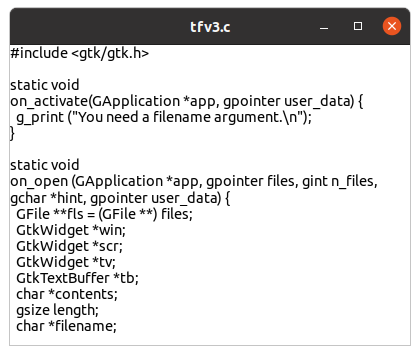
\includegraphics[width=6.3cm,height=5.325cm]{../image/screenshot_tfv3.png}
\caption{File viewer}
\end{figure}

The function \passthrough{\lstinline!main!} has only two changes from
the previous version.

\begin{itemize}
\tightlist
\item
  \passthrough{\lstinline!G\_APPLICATION\_DEFAULT\_FLAGS!} is replaced
  by \passthrough{\lstinline!G\_APPLICATION\_HANDLES\_OPEN!}
\item
  \passthrough{\lstinline!g\_signal\_connect (app, "open", G\_CALLBACK (app\_open), NULL)!}
  is added.
\end{itemize}

When the flag \passthrough{\lstinline!G\_APPLICATION\_HANDLES\_OPEN!} is
given to \passthrough{\lstinline!gtk\_application\_new!} function, the
application behaves like this:

\begin{itemize}
\tightlist
\item
  If the application is run without command line arguments, it emits
  ``activate'' signal when it is activated.
\item
  If the application is run with command line arguments, it emits
  ``open'' signal when it is activated.
\end{itemize}

The handler \passthrough{\lstinline!app\_activate!} becomes very simple.
It just outputs an error message and returns to the caller. Then the
application quits immediately because no window is created.

The main work is done in the handler
\passthrough{\lstinline!app\_open!}.

\begin{itemize}
\tightlist
\item
  Creates GtkApplicationWindow, GtkScrolledWindow, GtkTextView and
  GtkTextBuffer and connects them together
\item
  Sets wrap mode to \passthrough{\lstinline!GTK\_WRAP\_WORD\_CHAR!} in
  GtktextView
\item
  Sets GtkTextView to non-editable because the program isn't an editor
  but only a viewer
\item
  Reads the file and inserts the text into GtkTextBuffer (this will be
  explained later)
\item
  If the file is not opened, outputs an error message and destroys the
  window. This makes the application quit.
\end{itemize}

The following is the file reading part of the program.

\begin{lstlisting}[language=C]
if (g_file_load_contents (files[0], NULL, &contents, &length, NULL, &err)) {
  gtk_text_buffer_set_text (tb, contents, length);
  g_free (contents);
  if ((filename = g_file_get_basename (files[0])) != NULL) {
    gtk_window_set_title (GTK_WINDOW (win), filename);
    g_free (filename);
  }
  gtk_window_present (GTK_WINDOW (win));
} else {
  g_printerr ("%s.\n", err->message);
  g_error_free (err);
  gtk_window_destroy (GTK_WINDOW (win));
}
\end{lstlisting}

The function \passthrough{\lstinline!g\_file\_load\_contents!} loads the
file contents into a temporary buffer, which is automatically allocated
and sets \passthrough{\lstinline!contents!} to point the buffer. The
length of the buffer is assigned to \passthrough{\lstinline!length!}. It
returns \passthrough{\lstinline!TRUE!} if the file's contents are
successfully loaded. If an error occurs, it returns
\passthrough{\lstinline!FALSE!} and sets the variable
\passthrough{\lstinline!err!} to point a newly created GError structure.
The caller takes ownership of the GError structure and is responsible
for freeing it. If you want to know the details about
g\_file\_load\_contents, see
\href{https://docs.gtk.org/gio/method.File.load_contents.html}{g file
load contents}.

If it has successfully read the file, it inserts the contents into
GtkTextBuffer, frees the temporary buffer pointed by
\passthrough{\lstinline!contents!}, sets the title of the window, frees
the memories pointed by \passthrough{\lstinline!filename!} and then
shows the window.

If it fails, \passthrough{\lstinline!g\_file\_load\_contents!} sets
\passthrough{\lstinline!err!} to point a newly created GError structure.
The structure is:

\begin{lstlisting}[language=C]
struct GError {
  GQuark domain;
  int code;
  char* message;
}
\end{lstlisting}

The \passthrough{\lstinline!message!} member is used most often. It
points an error message. A function
\passthrough{\lstinline!g\_error\_free!} is used to free the memory of
the structure. See
\href{https://docs.gtk.org/glib/struct.Error.html}{GError}.

The program above outputs an error message, frees
\passthrough{\lstinline!err!} and destroys the window and finally make
the program quit.

\subsection{GtkNotebook}\label{gtknotebook}

GtkNotebook is a container widget that contains multiple widgets with
tabs. It shows only one child at a time. Another child will be shown
when its tab is clicked.

\begin{figure}
\centering
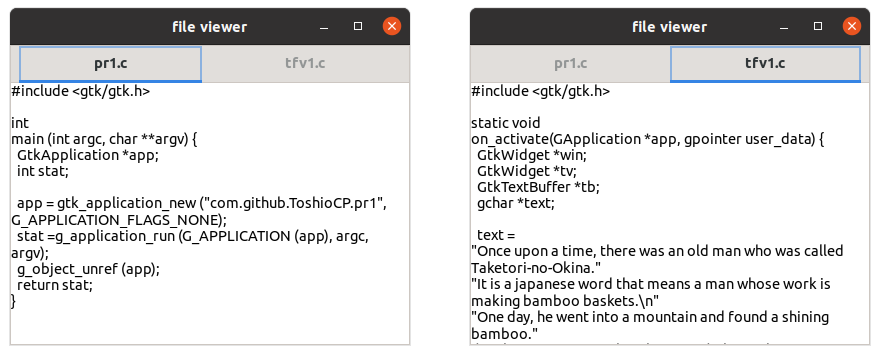
\includegraphics[width=13.2cm,height=5.325cm]{../image/screenshot_gtk_notebook.png}
\caption{GtkNotebook}
\end{figure}

The left image is the window at the startup. The file
\passthrough{\lstinline!pr1.c!} is shown and its filename is in the left
tab. After clicking on the right tab, the contents of the file
\passthrough{\lstinline!tfv1.c!} is shown (the right image).

The following is \passthrough{\lstinline!tfv4.c!}. It has GtkNoteBook
widget. It is inserted as a child of GtkApplicationWindow and contains
multiple GtkScrolledWindow.

\begin{lstlisting}[language=C, numbers=left]
#include <gtk/gtk.h>

static void
app_activate (GApplication *app) {
  g_printerr ("You need filename arguments.\n");
}

static void
app_open (GApplication *app, GFile ** files, gint n_files, gchar *hint) {
  GtkWidget *win;
  GtkWidget *nb;
  GtkWidget *lab;
  GtkNotebookPage *nbp;
  GtkWidget *scr;
  GtkWidget *tv;
  GtkTextBuffer *tb;
  char *contents;
  gsize length;
  char *filename;
  int i;
  GError *err = NULL;

  win = gtk_application_window_new (GTK_APPLICATION (app));
  gtk_window_set_title (GTK_WINDOW (win), "file viewer");
  gtk_window_set_default_size (GTK_WINDOW (win), 600, 400);
  nb = gtk_notebook_new ();
  gtk_window_set_child (GTK_WINDOW (win), nb);

  for (i = 0; i < n_files; i++) {
    if (g_file_load_contents (files[i], NULL, &contents, &length, NULL, &err)) {
      scr = gtk_scrolled_window_new ();
      tv = gtk_text_view_new ();
      tb = gtk_text_view_get_buffer (GTK_TEXT_VIEW (tv));
      gtk_text_view_set_wrap_mode (GTK_TEXT_VIEW (tv), GTK_WRAP_WORD_CHAR);
      gtk_text_view_set_editable (GTK_TEXT_VIEW (tv), FALSE);
      gtk_scrolled_window_set_child (GTK_SCROLLED_WINDOW (scr), tv);

      gtk_text_buffer_set_text (tb, contents, length);
      g_free (contents);
      if ((filename = g_file_get_basename (files[i])) != NULL) {
        lab = gtk_label_new (filename);
        g_free (filename);
      } else
        lab = gtk_label_new ("");
      gtk_notebook_append_page (GTK_NOTEBOOK (nb), scr, lab);
      nbp = gtk_notebook_get_page (GTK_NOTEBOOK (nb), scr);
      g_object_set (nbp, "tab-expand", TRUE, NULL);
    } else {
      g_printerr ("%s.\n", err->message);
      g_clear_error (&err);
    }
  }
  if (gtk_notebook_get_n_pages (GTK_NOTEBOOK (nb)) > 0)
    gtk_window_present (GTK_WINDOW (win));
  else
    gtk_window_destroy (GTK_WINDOW (win));
}

int
main (int argc, char **argv) {
  GtkApplication *app;
  int stat;

  app = gtk_application_new ("com.github.ToshioCP.tfv4", G_APPLICATION_HANDLES_OPEN);
  g_signal_connect (app, "activate", G_CALLBACK (app_activate), NULL);
  g_signal_connect (app, "open", G_CALLBACK (app_open), NULL);
  stat = g_application_run (G_APPLICATION (app), argc, argv);
  g_object_unref (app);
  return stat;
}
\end{lstlisting}

Most of the changes are in the function
\passthrough{\lstinline!app\_open!}. The numbers at the left of the
following items are line numbers in the source code.

\begin{itemize}
\tightlist
\item
  11-13: Variables \passthrough{\lstinline!nb!},
  \passthrough{\lstinline!lab!} and \passthrough{\lstinline!nbp!} are
  defined. They point GtkNotebook, GtkLabel and GtkNotebookPage
  respectively.
\item
  24: The window's title is set to ``file viewer''.
\item
  25: The default size of the window is 600x400.
\item
  26-27: GtkNotebook is created and inserted to the GtkApplicationWindow
  as a child.
\item
  29-57: For-loop. The variable \passthrough{\lstinline!files[i]!}
  points i-th GFile, which is created by the GtkApplication from the
  i-th command line argument.
\item
  31-36: GtkScrollledWindow, GtkTextView are created. GtkTextBuffer is
  got from the GtkTextView. The GtkTextView is connected to the
  GtkScrolledWindow as a child.
\item
  38-39: inserts the contents of the file into GtkTextBuffer and frees
  the memory pointed by \passthrough{\lstinline!contents!}.
\item
  40-42: If the filename is taken from the GFile, GtkLabel is created
  with the filename. The string \passthrough{\lstinline!filename!} is
  freed..
\item
  43-44: If it fails to take the filename, empty string GtkLabel is
  created.
\item
  45-46: Appends a GtkScrolledWindow to the GtkNotebook as a child. And
  the GtkLabel is set as the child's tab. At the same time, a
  GtkNoteBookPage is created automatically. The function
  \passthrough{\lstinline!gtk\_notebook\_get\_page!} returns the
  GtkNotebookPage of the child (GtkScrolledWindow).
\item
  47: GtkNotebookPage has ``tab-expand'' property. If it is set to TRUE
  then the tab expands horizontally as long as possible. If it is FALSE,
  then the width of the tab is determined by the size of the label.
  \passthrough{\lstinline!g\_object\_set!} is a general function to set
  properties of objects. See
  \href{https://docs.gtk.org/gobject/method.Object.set.html}{GObject API
  Reference -- g\_object\_set}.
\item
  48-50: If it fails to read the file, the error message is shown. The
  function \passthrough{\lstinline!g\_clear\_error (\&err)!} works like
  \passthrough{\lstinline!g\_error\_free (err); err = NULL!}.
\item
  53-56: If at least one page exists, the window is shown. Otherwise,
  the window is destroyed and the application quits.
\end{itemize}

  \section{Defining a final class}\label{defining-a-final-class}

\subsection{A very simple editor}\label{a-very-simple-editor}

We made a very simple file viewer in the previous section. Now we go on
to rewrite it and turn it into very simple editor. Its source file is
\passthrough{\lstinline!tfe1.c!} (text file editor 1) under
\passthrough{\lstinline!tfe!} directory.

GtkTextView is a multi-line editor. So, we don't need to write the
editor from scratch. We just add two things to the file viewer:

\begin{itemize}
\tightlist
\item
  Pointers to GFile instances.
\item
  A text-save function.
\end{itemize}

There are a couple of ways to store the pointers.

\begin{itemize}
\tightlist
\item
  Use global variables
\item
  Make a child class of GtkTextView and its each instance holds a
  pointer to the GFile instance.
\end{itemize}

Using global variables is easy to implement. Define a sufficient size
pointer array to GFile. For example,

\begin{lstlisting}[language=C]
GFile *f[20];
\end{lstlisting}

The variable \passthrough{\lstinline!f[i]!} corresponds to the file
associated with the i-th GtkNotebookPage.

However, There are two problems. The first is the size of the array. If
a user gives too many arguments (more than 20 in the example above), it
is impossible to store all the pointers to the GFile instances. The
second is difficulty to maintain the program. We have a small program so
far. But, the more you develop the program, the bigger its size grows.
Generally speaking, it is very difficult to maintain global variables in
a big program. When you check the global variable, you need to check all
the codes that use the variable.

Making a child class is a good idea in terms of maintenance. And we
prefer it rather than a global variable.

Be careful that we are thinking about ``child class'', not ``child
widget''. Child class and child widget are totally different. Class is a
term of GObject system. If you are not familiar with GObject, see:

\begin{itemize}
\tightlist
\item
  \href{https://docs.gtk.org/gobject/}{GObject API reference}
\item
  \href{https://toshiocp.github.io/Gobject-tutorial/}{GObject tutorial
  for beginners}
\end{itemize}

A child class inherits everything from the parent and, in addition,
extends its performance. We will define TfeTextView as a child class of
GtkTextView. It has everything that GtkTextView has and adds a pointer
to a GFile.

\begin{figure}
\centering
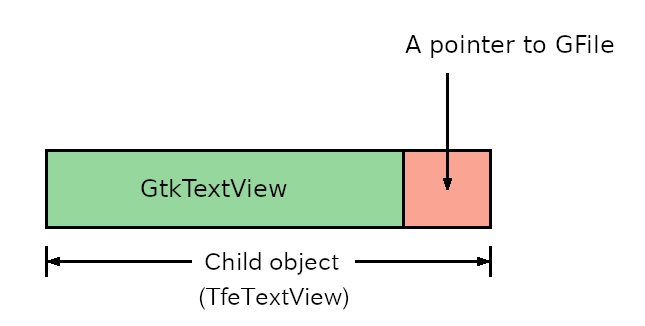
\includegraphics[width=9.675cm,height=4.89cm]{../image/child.png}
\caption{Child object of GtkTextView}
\end{figure}

\subsection{How to define a child class of
GtkTextView}\label{how-to-define-a-child-class-of-gtktextview}

You need to know GObject system convention. First, look at the program
below.

\begin{lstlisting}[language=C]
#define TFE_TYPE_TEXT_VIEW tfe_text_view_get_type ()
G_DECLARE_FINAL_TYPE (TfeTextView, tfe_text_view, TFE, TEXT_VIEW, GtkTextView)

struct _TfeTextView
{
  GtkTextView parent;
  GFile *file;
};

G_DEFINE_FINAL_TYPE (TfeTextView, tfe_text_view, GTK_TYPE_TEXT_VIEW);

static void
tfe_text_view_init (TfeTextView *tv) {
}

static void
tfe_text_view_class_init (TfeTextViewClass *class) {
}

void
tfe_text_view_set_file (TfeTextView *tv, GFile *f) {
  tv -> file = f;
}

GFile *
tfe_text_view_get_file (TfeTextView *tv) {
  return tv -> file;
}

GtkWidget *
tfe_text_view_new (void) {
  return GTK_WIDGET (g_object_new (TFE_TYPE_TEXT_VIEW, NULL));
}
\end{lstlisting}

\begin{itemize}
\tightlist
\item
  TfeTextView is divided into two parts. Tfe and TextView. Tfe is called
  prefix or namespace. TextView is called object.
\item
  There are three different identifier patterns. TfeTextView (camel
  case), tfe\_text\_view (this is used for functions) and
  TFE\_TEXT\_VIEW (This is used to cast a object to TfeTextView).
\item
  First, define \passthrough{\lstinline!TFE\_TYPE\_TEXT\_VIEW!} macro as
  \passthrough{\lstinline!tfe\_text\_view\_get\_type ()!}. The name is
  always (prefix)\_TYPE\_(object) and the letters are upper case. And
  the replacement text is always (prefix)\_(object)\_get\_type () and
  the letters are lower case. This definition is put before
  \passthrough{\lstinline!G\_DECLARE\_FINAL\_TYPE!} macro.
\item
  The arguments of \passthrough{\lstinline!G\_DECLARE\_FINAL\_TYPE!}
  macro are the child class name in camel case, lower case with
  underscore, prefix (upper case), object (upper case with underscore)
  and parent class name (camel case). The following two C structures are
  declared in the expansion of the macro.

  \begin{itemize}
  \tightlist
  \item
    \passthrough{\lstinline!typedef struct \_TfeTextView TfeTextView!}
  \item
    \passthrough{\lstinline!typedef struct \{GtkTextViewClass parent\_class; \} TfeTextViewClass;!}
  \end{itemize}
\item
  These declaration tells us that TfeTextView and TfeTextViewClass are C
  structures. ``TfeTextView'' has two meanings, class name and C
  structure name. The C structure TfeTextView is called object.
  Similarly, TfeTextViewClass is called class.
\item
  Declare the structure \passthrough{\lstinline!\_TfeTextView!}. The
  underscore is necessary. The first member is the parent object (C
  structure). Notice this is not a pointer but the object itself. The
  second member and after are members of the child object. TfeTextView
  structure has a pointer to a GFile instance as a member.
\item
  \passthrough{\lstinline!G\_DEFINE\_FINEL\_TYPE!} macro. The arguments
  are the child object name in camel case, lower case with underscore
  and parent object type (prefix)\_TYPE\_(module). This macro is mainly
  used to register the new class to the type system. Type system is a
  base system of GObject. Every class has its own type. The types of
  GObject, GtkWidget and TfeTextView are
  \passthrough{\lstinline!G\_TYPE\_OBJECT!},
  \passthrough{\lstinline!GTK\_TYPE\_WIDGET!} and
  \passthrough{\lstinline!TFE\_TYPE\_TEXT\_VIEW!} respectively. For
  example, \passthrough{\lstinline!TFE\_TYPE\_TEXT\_VIEW!} is a macro
  and it is expanded to a function
  \passthrough{\lstinline!tfe\_text\_view\_get\_type()!}. It returns a
  integer which is unique among all GObject system classes.
\item
  The instance init function
  \passthrough{\lstinline!tfe\_text\_view\_init!} is called when the
  instance is created. It is the same as a constructor in other object
  oriented languages.
\item
  The class init function
  \passthrough{\lstinline!tfe\_text\_view\_class\_init!} is called when
  the class is created.
\item
  Two functions \passthrough{\lstinline!tfe\_text\_view\_set\_file!} and
  \passthrough{\lstinline!tfe\_text\_view\_get\_file!} are public
  functions. Public functions are open and you can call them anywhere.
  They are the same as public method in other object oriented languages.
  \passthrough{\lstinline!tv!} is a pointer to the TfeTextView object (C
  structure). It has a member \passthrough{\lstinline!file!} and it is
  pointed by \passthrough{\lstinline!tv->file!}.
\item
  TfeTextView instance creation function is
  \passthrough{\lstinline!tfe\_text\_view\_new!}. Its name is
  (prefix)\_(object)\_new. It uses
  \passthrough{\lstinline!g\_object\_new!} function to create the
  instance. The arguments are (prefix)\_TYPE\_(object), a list to
  initialize properties and NULL. NULL is the end mark of the property
  list. No property is initialized here. And the return value is casted
  to GtkWidget.
\end{itemize}

This program shows the outline how to define a child class.

\subsection{Close-request signal}\label{close-request-signal}

Imagine that you are using this editor. First, you run the editor with
arguments. The arguments are filenames. The editor reads the files and
shows the window with the text of files in it. Then you edit the text.
After you finish editing, you click on the close button of the window
and quit the editor. The editor updates files just before the window
closes.

GtkWindow emits the ``close-request'' signal when the close button is
clicked. We will connect the signal and the handler
\passthrough{\lstinline!before\_close!}. (A handler is a C function
which is connected to a signal.) The function
\passthrough{\lstinline!before\_close!} is called when the signal
``close-request'' is emitted.

\begin{lstlisting}[language=C]
g_signal_connect (win, "close-request", G_CALLBACK (before_close), NULL);
\end{lstlisting}

The argument \passthrough{\lstinline!win!} is a GtkApplicationWindow, in
which the signal ``close-request'' is defined, and
\passthrough{\lstinline!before\_close!} is the handler. The
\passthrough{\lstinline!G\_CALLBACK!} cast is necessary for the handler.
The program of \passthrough{\lstinline!before\_close!} is as follows.

\begin{lstlisting}[language=C, numbers=left]
static gboolean
before_close (GtkWindow *win, GtkWidget *nb) {
  GtkWidget *scr;
  GtkWidget *tv;
  GFile *file;
  char *pathname;
  GtkTextBuffer *tb;
  GtkTextIter start_iter;
  GtkTextIter end_iter;
  char *contents;
  unsigned int n;
  unsigned int i;
  GError *err = NULL;

  n = gtk_notebook_get_n_pages (GTK_NOTEBOOK (nb));
  for (i = 0; i < n; ++i) {
    scr = gtk_notebook_get_nth_page (GTK_NOTEBOOK (nb), i);
    tv = gtk_scrolled_window_get_child (GTK_SCROLLED_WINDOW (scr));
    file = tfe_text_view_get_file (TFE_TEXT_VIEW (tv));
    tb = gtk_text_view_get_buffer (GTK_TEXT_VIEW (tv));
    gtk_text_buffer_get_bounds (tb, &start_iter, &end_iter);
    contents = gtk_text_buffer_get_text (tb, &start_iter, &end_iter, FALSE);
    if (! g_file_replace_contents (file, contents, strlen (contents), NULL, TRUE, G_FILE_CREATE_NONE, NULL, NULL, &err)) {
      g_printerr ("%s.\n", err->message);
      g_clear_error (&err);
    }
    g_free (contents);
    g_object_unref (file);
  }
  return FALSE;
}
\end{lstlisting}

The numbers on the left are line numbers.

\begin{itemize}
\tightlist
\item
  15: The number of note book pages is assigned to
  \passthrough{\lstinline!n!}.
\item
  16-29: For loop with regard to the index to each page.
\item
  17-19: \passthrough{\lstinline!scr!}, \passthrough{\lstinline!tv!} and
  \passthrough{\lstinline!file!} is assigned pointers to the
  GtkScrolledWindow, TfeTextView and GFile. The GFile of TfeTextView was
  stored when \passthrough{\lstinline!app\_open!} handler was called. It
  will be shown later.
\item
  20-22: \passthrough{\lstinline!tb!} is assigned the GtkTextBuffer of
  the TfeTextView. The contents of the buffer are accessed with
  iterators. Iterators points somewhere in the buffer. The function
  \passthrough{\lstinline!gtk\_text\_buffer\_get\_bounds!} assigns the
  start and end of the buffer to \passthrough{\lstinline!start\_iter!}
  and \passthrough{\lstinline!end\_iter!} respectively. Then the
  function \passthrough{\lstinline!gtk\_text\_buffer\_get\_text!}
  returns the text between \passthrough{\lstinline!start\_iter!} and
  \passthrough{\lstinline!end\_iter!}, which is the whole text in the
  buffer.
\item
  23-26: The text is saved to the file. If it fails, error messages are
  displayed. The GError instance must be freed and the pointer
  \passthrough{\lstinline!err!} needs to be NULL for the next run in the
  loop.
\item
  27: \passthrough{\lstinline!contents!} are freed.
\item
  28: GFile is useless. \passthrough{\lstinline!g\_object\_unref!}
  decreases the reference count of the GFile. Reference count will be
  explained in the later section. The reference count will be zero and
  the GFile instance will destroy itself.
\end{itemize}

\subsection{Source code of tfe1.c}\label{source-code-of-tfe1.c}

The following is the whole source code of
\passthrough{\lstinline!tfe1.c!}.

\begin{lstlisting}[language=C, numbers=left]
#include <gtk/gtk.h>

/* Define TfeTextView Widget which is the child class of GtkTextView */

#define TFE_TYPE_TEXT_VIEW tfe_text_view_get_type ()
G_DECLARE_FINAL_TYPE (TfeTextView, tfe_text_view, TFE, TEXT_VIEW, GtkTextView)

struct _TfeTextView
{
  GtkTextView parent;
  GFile *file;
};

G_DEFINE_FINAL_TYPE (TfeTextView, tfe_text_view, GTK_TYPE_TEXT_VIEW);

static void
tfe_text_view_init (TfeTextView *tv) {
  tv->file = NULL;
}

static void
tfe_text_view_class_init (TfeTextViewClass *class) {
}

void
tfe_text_view_set_file (TfeTextView *tv, GFile *f) {
  tv->file = f;
}

GFile *
tfe_text_view_get_file (TfeTextView *tv) {
  return tv -> file;
}

GtkWidget *
tfe_text_view_new (void) {
  return GTK_WIDGET (g_object_new (TFE_TYPE_TEXT_VIEW, NULL));
}

/* ---------- end of the definition of TfeTextView ---------- */

static gboolean
before_close (GtkWindow *win, GtkWidget *nb) {
  GtkWidget *scr;
  GtkWidget *tv;
  GFile *file;
  char *pathname;
  GtkTextBuffer *tb;
  GtkTextIter start_iter;
  GtkTextIter end_iter;
  char *contents;
  unsigned int n;
  unsigned int i;
  GError *err = NULL;

  n = gtk_notebook_get_n_pages (GTK_NOTEBOOK (nb));
  for (i = 0; i < n; ++i) {
    scr = gtk_notebook_get_nth_page (GTK_NOTEBOOK (nb), i);
    tv = gtk_scrolled_window_get_child (GTK_SCROLLED_WINDOW (scr));
    file = tfe_text_view_get_file (TFE_TEXT_VIEW (tv));
    tb = gtk_text_view_get_buffer (GTK_TEXT_VIEW (tv));
    gtk_text_buffer_get_bounds (tb, &start_iter, &end_iter);
    contents = gtk_text_buffer_get_text (tb, &start_iter, &end_iter, FALSE);
    if (! g_file_replace_contents (file, contents, strlen (contents), NULL, TRUE, G_FILE_CREATE_NONE, NULL, NULL, &err)) {
      g_printerr ("%s.\n", err->message);
      g_clear_error (&err);
    }
    g_free (contents);
    g_object_unref (file);
  }
  return FALSE;
}

static void
app_activate (GApplication *app) {
  g_print ("You need to give filenames as arguments.\n");
}

static void
app_open (GApplication *app, GFile ** files, gint n_files, gchar *hint) {
  GtkWidget *win;
  GtkWidget *nb;
  GtkWidget *lab;
  GtkNotebookPage *nbp;
  GtkWidget *scr;
  GtkWidget *tv;
  GtkTextBuffer *tb;
  char *contents;
  gsize length;
  char *filename;
  int i;
  GError *err = NULL;

  win = gtk_application_window_new (GTK_APPLICATION (app));
  gtk_window_set_title (GTK_WINDOW (win), "file editor");
  gtk_window_set_default_size (GTK_WINDOW (win), 600, 400);

  nb = gtk_notebook_new ();
  gtk_window_set_child (GTK_WINDOW (win), nb);

  for (i = 0; i < n_files; i++) {
    if (g_file_load_contents (files[i], NULL, &contents, &length, NULL, &err)) {
      scr = gtk_scrolled_window_new ();
      tv = tfe_text_view_new ();
      tb = gtk_text_view_get_buffer (GTK_TEXT_VIEW (tv));
      gtk_text_view_set_wrap_mode (GTK_TEXT_VIEW (tv), GTK_WRAP_WORD_CHAR);
      gtk_scrolled_window_set_child (GTK_SCROLLED_WINDOW (scr), tv);

      tfe_text_view_set_file (TFE_TEXT_VIEW (tv),  g_file_dup (files[i]));
      gtk_text_buffer_set_text (tb, contents, length);
      g_free (contents);
      filename = g_file_get_basename (files[i]);
      lab = gtk_label_new (filename);
      gtk_notebook_append_page (GTK_NOTEBOOK (nb), scr, lab);
      nbp = gtk_notebook_get_page (GTK_NOTEBOOK (nb), scr);
      g_object_set (nbp, "tab-expand", TRUE, NULL);
      g_free (filename);
    } else {
      g_printerr ("%s.\n", err->message);
      g_clear_error (&err);
    }
  }
  if (gtk_notebook_get_n_pages (GTK_NOTEBOOK (nb)) > 0) {
    g_signal_connect (win, "close-request", G_CALLBACK (before_close), nb);
    gtk_window_present (GTK_WINDOW (win));
  } else
    gtk_window_destroy (GTK_WINDOW (win));
}

int
main (int argc, char **argv) {
  GtkApplication *app;
  int stat;

  app = gtk_application_new ("com.github.ToshioCP.tfe1", G_APPLICATION_HANDLES_OPEN);
  g_signal_connect (app, "activate", G_CALLBACK (app_activate), NULL);
  g_signal_connect (app, "open", G_CALLBACK (app_open), NULL);
  stat =g_application_run (G_APPLICATION (app), argc, argv);
  g_object_unref (app);
  return stat;
}
\end{lstlisting}

\begin{itemize}
\tightlist
\item
  109: The GFile pointer of the TfeTextView is set to the copy of
  \passthrough{\lstinline!files[i]!}, which is a GFile created with the
  command line argument. The GFile will be destroyed by the system
  later. So it needs to be copied before the assignment.
  \passthrough{\lstinline!g\_file\_dup!} duplicates the GFile. Note:
  GFile is \emph{not} thread safe. Duplicating GFile avoids a trouble
  comes from the different thread.
\item
  124: The ``close-request'' signal is connected to
  \passthrough{\lstinline!before\_close!} handler. The fourth argument
  is called ``user data'' and it will be the second argument of the
  signal handler. So, \passthrough{\lstinline!nb!} is given to
  \passthrough{\lstinline!before\_close!} as the second argument.
\end{itemize}

Now it's time to compile and run.

\begin{lstlisting}
$ cd src/tfe
$ comp tfe1
$ ./a.out taketori.txt`.
\end{lstlisting}

Modify the contents and close the window. Make sure that the file is
modified.

Now we got a very simple editor. It's not smart. We need more features
like open, save, saveas, change font and so on. We will add them in the
next section and after.

  \section{GtkBuilder and UI file}\label{gtkbuilder-and-ui-file}

\subsection{New, Open and Save button}\label{new-open-and-save-button}

We made very simple editor in the previous section. It reads files at
the start and writes them out at the end of the program. It works, but
is not so good. It would be better if we had ``New'', ``Open'', ``Save''
and ``Close'' buttons. This section describes how to put those buttons
into the window.

\begin{figure}
\centering
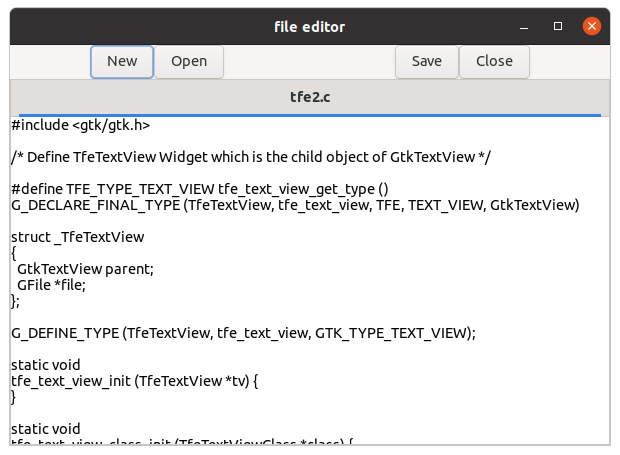
\includegraphics[width=9.3cm,height=6.825cm]{../image/screenshot_tfe2.png}
\caption{Screenshot of the file editor}
\end{figure}

The screenshot above shows the layout. The function
\passthrough{\lstinline!app\_open!} in the source code
\passthrough{\lstinline!tfe2.c!} is as follows.

\begin{lstlisting}[language=C, numbers=left]
static void
app_open (GApplication *app, GFile ** files, gint n_files, gchar *hint) {
  GtkWidget *win;
  GtkWidget *nb;
  GtkWidget *lab;
  GtkNotebookPage *nbp;
  GtkWidget *scr;
  GtkWidget *tv;
  GtkTextBuffer *tb;
  char *contents;
  gsize length;
  char *filename;
  int i;
  GError *err = NULL;

  GtkWidget *boxv;
  GtkWidget *boxh;
  GtkWidget *dmy1;
  GtkWidget *dmy2;
  GtkWidget *dmy3;
  GtkWidget *btnn; /* button for new */
  GtkWidget *btno; /* button for open */
  GtkWidget *btns; /* button for save */
  GtkWidget *btnc; /* button for close */

  win = gtk_application_window_new (GTK_APPLICATION (app));
  gtk_window_set_title (GTK_WINDOW (win), "file editor");
  gtk_window_set_default_size (GTK_WINDOW (win), 600, 400);

  boxv = gtk_box_new (GTK_ORIENTATION_VERTICAL, 0);
  gtk_window_set_child (GTK_WINDOW (win), boxv);

  boxh = gtk_box_new (GTK_ORIENTATION_HORIZONTAL, 0);
  gtk_box_append (GTK_BOX (boxv), boxh);

  dmy1 = gtk_label_new(NULL); /* dummy label for left space */
  gtk_label_set_width_chars (GTK_LABEL (dmy1), 10);
  dmy2 = gtk_label_new(NULL); /* dummy label for center space */
  gtk_widget_set_hexpand (dmy2, TRUE);
  dmy3 = gtk_label_new(NULL); /* dummy label for right space */
  gtk_label_set_width_chars (GTK_LABEL (dmy3), 10);
  btnn = gtk_button_new_with_label ("New");
  btno = gtk_button_new_with_label ("Open");
  btns = gtk_button_new_with_label ("Save");
  btnc = gtk_button_new_with_label ("Close");

  gtk_box_append (GTK_BOX (boxh), dmy1);
  gtk_box_append (GTK_BOX (boxh), btnn);
  gtk_box_append (GTK_BOX (boxh), btno);
  gtk_box_append (GTK_BOX (boxh), dmy2);
  gtk_box_append (GTK_BOX (boxh), btns);
  gtk_box_append (GTK_BOX (boxh), btnc);
  gtk_box_append (GTK_BOX (boxh), dmy3);

  nb = gtk_notebook_new ();
  gtk_widget_set_hexpand (nb, TRUE);
  gtk_widget_set_vexpand (nb, TRUE);
  gtk_box_append (GTK_BOX (boxv), nb);

  for (i = 0; i < n_files; i++) {
    if (g_file_load_contents (files[i], NULL, &contents, &length, NULL, &err)) {
      scr = gtk_scrolled_window_new ();
      tv = tfe_text_view_new ();
      tb = gtk_text_view_get_buffer (GTK_TEXT_VIEW (tv));
      gtk_text_view_set_wrap_mode (GTK_TEXT_VIEW (tv), GTK_WRAP_WORD_CHAR);
      gtk_scrolled_window_set_child (GTK_SCROLLED_WINDOW (scr), tv);

      tfe_text_view_set_file (TFE_TEXT_VIEW (tv),  g_file_dup (files[i]));
      gtk_text_buffer_set_text (tb, contents, length);
      g_free (contents);
      filename = g_file_get_basename (files[i]);
      lab = gtk_label_new (filename);
      gtk_notebook_append_page (GTK_NOTEBOOK (nb), scr, lab);
      nbp = gtk_notebook_get_page (GTK_NOTEBOOK (nb), scr);
      g_object_set (nbp, "tab-expand", TRUE, NULL);
      g_free (filename);
    } else {
      g_printerr ("%s.\n", err->message);
      g_clear_error (&err);
    }
  }
  if (gtk_notebook_get_n_pages (GTK_NOTEBOOK (nb)) > 0) {
    gtk_window_present (GTK_WINDOW (win));
  } else
    gtk_window_destroy (GTK_WINDOW (win));
}
\end{lstlisting}

The function \passthrough{\lstinline!app\_open!} builds the widgets in
the main application window.

\begin{itemize}
\tightlist
\item
  26-28: Creates a GtkApplicationWindow instance and sets the title and
  default size.
\item
  30-31: Creates a GtkBox instance \passthrough{\lstinline!boxv!}. It is
  a vertical box and a child of GtkApplicationWindow. It has two
  children. The first child is a horizontal box. The second child is a
  GtkNotebook.
\item
  33-34: Creates a GtkBox instance \passthrough{\lstinline!boxh!} and
  appends it to \passthrough{\lstinline!boxv!} as the first child.
\item
  36-41: Creates three dummy labels. The labels
  \passthrough{\lstinline!dmy1!} and \passthrough{\lstinline!dmy3!} has
  a character width of ten. The other label
  \passthrough{\lstinline!dmy2!} has hexpand property which is set to be
  TRUE. This makes the label expands horizontally as long as possible.
\item
  42-45: Creates four buttons.
\item
  47-53: Appends these GtkLabel and GtkButton to
  \passthrough{\lstinline!boxh!}.
\item
  55-58: Creates a GtkNotebook instance and sets hexpand and vexpand
  properties to be TRUE. This makes it expand horizontally and
  vertically as big as possible. It is appended to
  \passthrough{\lstinline!boxv!} as the second child.
\end{itemize}

The number of widget-build lines is 33(=58-26+1). We also needed many
variables (\passthrough{\lstinline!boxv!},
\passthrough{\lstinline!boxh!}, \passthrough{\lstinline!dmy1!}, \ldots)
and most of them used only for building the widgets. Are there any good
solution to reduce these works?

Gtk provides GtkBuilder. It reads user interface (UI) data and builds a
window. It reduces this cumbersome work.

\subsection{The UI File}\label{the-ui-file}

Look at the UI file \passthrough{\lstinline!tfe3.ui!} that defines
widget structure.

\begin{lstlisting}[language=XML, numbers=left]
<?xml version="1.0" encoding="UTF-8"?>
<interface>
  <object class="GtkApplicationWindow" id="win">
    <property name="title">file editor</property>
    <property name="default-width">600</property>
    <property name="default-height">400</property>
    <child>
      <object class="GtkBox">
        <property name="orientation">GTK_ORIENTATION_VERTICAL</property>
        <child>
          <object class="GtkBox">
            <property name="orientation">GTK_ORIENTATION_HORIZONTAL</property>
            <child>
              <object class="GtkLabel">
                <property name="width-chars">10</property>
              </object>
            </child>
            <child>
              <object class="GtkButton">
                <property name="label">New</property>
              </object>
            </child>
            <child>
              <object class="GtkButton">
                <property name="label">Open</property>
              </object>
            </child>
            <child>
              <object class="GtkLabel">
                <property name="hexpand">TRUE</property>
              </object>
            </child>
            <child>
              <object class="GtkButton">
                <property name="label">Save</property>
              </object>
            </child>
            <child>
              <object class="GtkButton">
                <property name="label">Close</property>
              </object>
            </child>
            <child>
              <object class="GtkLabel">
                <property name="width-chars">10</property>
              </object>
            </child>
          </object>
        </child>
        <child>
          <object class="GtkNotebook" id="nb">
            <property name="hexpand">TRUE</property>
            <property name="vexpand">TRUE</property>
          </object>
        </child>
      </object>
    </child>
  </object>
</interface>
\end{lstlisting}

The is a XML file. Tags begin with \passthrough{\lstinline!<!} and end
with \passthrough{\lstinline!>!}. There are two types of tags, the start
tag and the end tag. For example, \passthrough{\lstinline!<interface>!}
is a start tag and \passthrough{\lstinline!</interface>!} is an end tag.
The UI file begins and ends with interface tags. Some tags, for example
object tags, can have a class and id attributes in their start tag.

\begin{itemize}
\tightlist
\item
  1: XML declaration. It specifies that the XML version is 1.0 and the
  encoding is UTF-8.
\item
  3-6: An object tag with \passthrough{\lstinline!GtkApplicationWindow!}
  class and \passthrough{\lstinline!win!} id. This is the top level
  window. And the three properties of the window are defined. The
  \passthrough{\lstinline!title!} property is ``file editor'',
  \passthrough{\lstinline!default-width!} property is 600 and
  \passthrough{\lstinline!default-height!} property is 400.
\item
  7: Child tag means a child widget. For example, line 7 tells us that
  GtkBox object is a child widget of \passthrough{\lstinline!win!}.
\end{itemize}

Compare this ui file and the lines 26-58 in the
\passthrough{\lstinline!app\_open!} function of
\passthrough{\lstinline!tfe2.c!}. Both builds the same window with its
descendant widgets.

You can check the ui file with
\passthrough{\lstinline!gtk4-builder-tool!}.

\begin{itemize}
\tightlist
\item
  \passthrough{\lstinline!gtk4-builder-tool validate <ui file name>!}
  validates the ui file. If the ui file includes some syntactical error,
  \passthrough{\lstinline!gtk4-builder-tool!} prints the error.
\item
  \passthrough{\lstinline!gtk4-builder-tool simplify <ui file name>!}
  simplifies the ui file and prints the result. If
  \passthrough{\lstinline!--replace!} option is given, it replaces the
  ui file with the simplified one. If the ui file specifies a value of
  property but it is default, then it will be removed. For example, the
  default orientation is horizontal so the simplification removes line
  12. And some values are simplified. For example, ``TRUE''and ``FALSE''
  becomes ``1'' and ``0'' respectively. However, ``TRUE'' or ``FALSE''
  is better for maintenance.
\end{itemize}

It is a good idea to check your ui file before compiling.

\subsection{GtkBuilder}\label{gtkbuilder}

GtkBuilder builds widgets based on a ui file.

\begin{lstlisting}[language=C]
GtkBuilder *build;

build = gtk_builder_new_from_file ("tfe3.ui");
win = GTK_WIDGET (gtk_builder_get_object (build, "win"));
gtk_window_set_application (GTK_WINDOW (win), GTK_APPLICATION (app));
nb = GTK_WIDGET (gtk_builder_get_object (build, "nb"));
g_object_unref(build);
\end{lstlisting}

The function \passthrough{\lstinline!gtk\_builder\_new\_from\_file!}
reads the file \passthrough{\lstinline!tfe3.ui!}. Then, it builds the
widgets and creates GtkBuilder object. All the widgets are connected
based on the parent-children relationship described in the ui file. We
can retrieve objects from the builder object with
\passthrough{\lstinline!gtk\_builder\_get\_object!} function. The top
level window, its id is ``win'' in the ui file, is taken and assigned to
the variable \passthrough{\lstinline!win!}, the application property of
which is set to \passthrough{\lstinline!app!} with the
\passthrough{\lstinline!gtk\_window\_set\_application!} function.
GtkNotebook with the id ``nb'' in the ui file is also taken and assigned
to the variable \passthrough{\lstinline!nb!}. After the window and
application are connected, GtkBuilder instance is useless. It is
released with \passthrough{\lstinline!g\_object\_unref!} function.

The ui file reduces lines in the C source file.

\begin{lstlisting}
$ cd tfe; diff tfe2.c tfe3.c
59a60
>   GtkBuilder *build;
61,104c62,66
<   GtkWidget *boxv;
<   GtkWidget *boxh;
<   GtkWidget *dmy1;
<   GtkWidget *dmy2;
<   GtkWidget *dmy3;
<   GtkWidget *btnn; /* button for new */
<   GtkWidget *btno; /* button for open */
<   GtkWidget *btns; /* button for save */
<   GtkWidget *btnc; /* button for close */
< 
<   win = gtk_application_window_new (GTK_APPLICATION (app));
<   gtk_window_set_title (GTK_WINDOW (win), "file editor");
<   gtk_window_set_default_size (GTK_WINDOW (win), 600, 400);
< 
<   boxv = gtk_box_new (GTK_ORIENTATION_VERTICAL, 0);
<   gtk_window_set_child (GTK_WINDOW (win), boxv);
< 
<   boxh = gtk_box_new (GTK_ORIENTATION_HORIZONTAL, 0);
<   gtk_box_append (GTK_BOX (boxv), boxh);
< 
<   dmy1 = gtk_label_new(NULL); /* dummy label for left space */
<   gtk_label_set_width_chars (GTK_LABEL (dmy1), 10);
<   dmy2 = gtk_label_new(NULL); /* dummy label for center space */
<   gtk_widget_set_hexpand (dmy2, TRUE);
<   dmy3 = gtk_label_new(NULL); /* dummy label for right space */
<   gtk_label_set_width_chars (GTK_LABEL (dmy3), 10);
<   btnn = gtk_button_new_with_label ("New");
<   btno = gtk_button_new_with_label ("Open");
<   btns = gtk_button_new_with_label ("Save");
<   btnc = gtk_button_new_with_label ("Close");
< 
<   gtk_box_append (GTK_BOX (boxh), dmy1);
<   gtk_box_append (GTK_BOX (boxh), btnn);
<   gtk_box_append (GTK_BOX (boxh), btno);
<   gtk_box_append (GTK_BOX (boxh), dmy2);
<   gtk_box_append (GTK_BOX (boxh), btns);
<   gtk_box_append (GTK_BOX (boxh), btnc);
<   gtk_box_append (GTK_BOX (boxh), dmy3);
< 
<   nb = gtk_notebook_new ();
<   gtk_widget_set_hexpand (nb, TRUE);
<   gtk_widget_set_vexpand (nb, TRUE);
<   gtk_box_append (GTK_BOX (boxv), nb);
< 
---
>   build = gtk_builder_new_from_file ("tfe3.ui");
>   win = GTK_WIDGET (gtk_builder_get_object (build, "win"));
>   gtk_window_set_application (GTK_WINDOW (win), GTK_APPLICATION (app));
>   nb = GTK_WIDGET (gtk_builder_get_object (build, "nb"));
>   g_object_unref(build);
138c100
<   app = gtk_application_new ("com.github.ToshioCP.tfe2", G_APPLICATION_HANDLES_OPEN);
---
>   app = gtk_application_new ("com.github.ToshioCP.tfe3", G_APPLICATION_HANDLES_OPEN);
144a107
> 
\end{lstlisting}

\passthrough{\lstinline!61,104c62,66!} means that 44 (=104-61+1) lines
are changed to 5 (=66-62+1) lines. Therefore, 39 lines are reduced.
Using ui file not only shortens C source files, but also makes the
widgets structure clear.

Now I'll show you \passthrough{\lstinline!app\_open!} function in the C
file \passthrough{\lstinline!tfe3.c!}.

\begin{lstlisting}[language=C, numbers=left]
static void
app_open (GApplication *app, GFile ** files, gint n_files, gchar *hint) {
  GtkWidget *win;
  GtkWidget *nb;
  GtkWidget *lab;
  GtkNotebookPage *nbp;
  GtkWidget *scr;
  GtkWidget *tv;
  GtkTextBuffer *tb;
  char *contents;
  gsize length;
  char *filename;
  int i;
  GError *err = NULL;
  GtkBuilder *build;

  build = gtk_builder_new_from_file ("tfe3.ui");
  win = GTK_WIDGET (gtk_builder_get_object (build, "win"));
  gtk_window_set_application (GTK_WINDOW (win), GTK_APPLICATION (app));
  nb = GTK_WIDGET (gtk_builder_get_object (build, "nb"));
  g_object_unref(build);
  for (i = 0; i < n_files; i++) {
    if (g_file_load_contents (files[i], NULL, &contents, &length, NULL, &err)) {
      scr = gtk_scrolled_window_new ();
      tv = tfe_text_view_new ();
      tb = gtk_text_view_get_buffer (GTK_TEXT_VIEW (tv));
      gtk_text_view_set_wrap_mode (GTK_TEXT_VIEW (tv), GTK_WRAP_WORD_CHAR);
      gtk_scrolled_window_set_child (GTK_SCROLLED_WINDOW (scr), tv);

      tfe_text_view_set_file (TFE_TEXT_VIEW (tv),  g_file_dup (files[i]));
      gtk_text_buffer_set_text (tb, contents, length);
      g_free (contents);
      filename = g_file_get_basename (files[i]);
      lab = gtk_label_new (filename);
      gtk_notebook_append_page (GTK_NOTEBOOK (nb), scr, lab);
      nbp = gtk_notebook_get_page (GTK_NOTEBOOK (nb), scr);
      g_object_set (nbp, "tab-expand", TRUE, NULL);
      g_free (filename);
    } else {
      g_printerr ("%s.\n", err->message);
      g_clear_error (&err);
    }
  }
  if (gtk_notebook_get_n_pages (GTK_NOTEBOOK (nb)) > 0) {
    gtk_window_present (GTK_WINDOW (win));
  } else
    gtk_window_destroy (GTK_WINDOW (win));
}
\end{lstlisting}

The whole source code of \passthrough{\lstinline!tfe3.c!} is stored in
the src/tfe directory.

\subsubsection{Using ui string}\label{using-ui-string}

GtkBuilder can build widgets with string. Use
\passthrough{\lstinline!gtk\_builder\_new\_from\_string!} instead of
\passthrough{\lstinline!gtk\_builder\_new\_from\_file!}.

\begin{lstlisting}[language=C]
char *uistring;

uistring =
"<interface>"
  "<object class="GtkApplicationWindow" id="win">"
    "<property name=\"title\">file editor</property>"
    "<property name=\"default-width\">600</property>"
    "<property name=\"default-height\">400</property>"
    "<child>"
      "<object class=\"GtkBox\">"
        "<property name="orientation">GTK_ORIENTATION_VERTICAL</property>"
... ... ...
... ... ...
"</interface>";

build = gtk_builder_new_from_string (uistring, -1);
\end{lstlisting}

This method has an advantage and disadvantage. The advantage is that the
ui string is written in the source code. So, no ui file is needed on
runtime. The disadvantage is that writing C string is a bit bothersome
because of the double quotes. If you want to use this method, you should
write a script that transforms ui file into C-string.

\begin{itemize}
\tightlist
\item
  Add backslash before each double quote.
\item
  Add double quotes at the left and right of the string in each line.
\end{itemize}

\subsubsection{Gresource}\label{gresource}

Gresource is similar to string. But Gresource is compressed binary data,
not text data. And there's a compiler that compiles ui file into
Gresource. It can compile not only text files but also binary files such
as images, sounds and so on. And after compilation, it bundles them up
into one Gresource object.

An xml file is necessary for the resource compiler
\passthrough{\lstinline!glib-compile-resources!}. It describes resource
files.

\begin{lstlisting}[language=XML, numbers=left]
<?xml version="1.0" encoding="UTF-8"?>
<gresources>
  <gresource prefix="/com/github/ToshioCP/tfe3">
    <file>tfe3.ui</file>
  </gresource>
</gresources>
\end{lstlisting}

\begin{itemize}
\tightlist
\item
  2: \passthrough{\lstinline!gresources!} tag can include multiple
  gresources (gresource tags). However, this xml has only one gresource.
\item
  3: The gresource has a prefix
  \passthrough{\lstinline!/com/github/ToshioCP/tfe3!}.
\item
  4: The name of the gresource is \passthrough{\lstinline!tfe3.ui!}. The
  resource will be pointed with
  \passthrough{\lstinline!/com/github/ToshioCP/tfe3/tfe3.ui!} by
  GtkBuilder. The pattern is ``prefix'' + ``name''. If you want to add
  more files, insert them between line 4 and 5.
\end{itemize}

Save this xml text to \passthrough{\lstinline!tfe3.gresource.xml!}. The
gresource compiler \passthrough{\lstinline!glib-compile-resources!}
shows its usage with the argument \passthrough{\lstinline!--help!}.

\begin{lstlisting}
$ glib-compile-resources --help
Usage:
  glib-compile-resources [OPTION..] FILE

Compile a resource specification into a resource file.
Resource specification files have the extension .gresource.xml,
and the resource file have the extension called .gresource.

Help Options:
  -h, --help                   Show help options

Application Options:
  --version                    Show program version and exit
  --target=FILE                Name of the output file
  --sourcedir=DIRECTORY        The directories to load files referenced in FILE from (default: current directory)
  --generate                   Generate output in the format selected for by the target filename extension
  --generate-header            Generate source header
  --generate-source            Generate source code used to link in the resource file into your code
  --generate-dependencies      Generate dependency list
  --dependency-file=FILE       Name of the dependency file to generate
  --generate-phony-targets     Include phony targets in the generated dependency file
  --manual-register            Don't automatically create and register resource
  --internal                   Don't export functions; declare them G_GNUC_INTERNAL
  --external-data              Don't embed resource data in the C file; assume it's linked externally instead
  --c-name                     C identifier name used for the generated source code
  -C, --compiler               The target C compiler (default: the CC environment variable)
\end{lstlisting}

Now run the compiler.

\begin{lstlisting}
$ glib-compile-resources tfe3.gresource.xml --target=resources.c --generate-source
\end{lstlisting}

Then a C source file \passthrough{\lstinline!resources.c!} is generated.
Modify \passthrough{\lstinline!tfe3.c!} and save it as
\passthrough{\lstinline!tfe3\_r.c!}.

\begin{lstlisting}[language=C]
#include "resources.c"
... ... ...
... ... ...
build = gtk_builder_new_from_resource ("/com/github/ToshioCP/tfe3/tfe3.ui");
... ... ...
... ... ...
\end{lstlisting}

The function \passthrough{\lstinline!gtk\_builder\_new\_from\_resource!}
builds widgets from a resource.

Then, compile and run it.

\begin{lstlisting}
$ comp tfe3_r
$ ./a.out tfe2.c
\end{lstlisting}

A window appears and it is the same as the screenshot at the beginning
of this page.

Generally, resource is the best way for C language. If you use other
languages like Ruby, string is better than resource.

  \section{Build system}\label{build-system}

\subsection{Managing big source files}\label{managing-big-source-files}

We've compiled a small editor so far. The program is also small and not
complicated yet. But if it grows bigger, it will be difficult to
maintain. So, we should do the followings now.

\begin{itemize}
\tightlist
\item
  We've had only one C source file and put everything in it. We need to
  divide it and sort them out.
\item
  There are two compilers, \passthrough{\lstinline!gcc!} and
  \passthrough{\lstinline!glib-compile-resources!}. We should control
  them by one building tool.
\end{itemize}

\subsection{Divide a C source file into two
parts.}\label{divide-a-c-source-file-into-two-parts.}

When you divide C source file into several parts, each file should
contain one thing. For example, our source has two things, the
definition of TfeTextView and functions related to GtkApplication and
GtkApplicationWindow. It is a good idea to separate them into two files,
\passthrough{\lstinline!tfetextview.c!} and
\passthrough{\lstinline!tfe.c!}.

\begin{itemize}
\tightlist
\item
  \passthrough{\lstinline!tfetextview.c!} includes the definition and
  functions of TfeTextView.
\item
  \passthrough{\lstinline!tfe.c!} includes functions like
  \passthrough{\lstinline!main!},
  \passthrough{\lstinline!app\_activate!},
  \passthrough{\lstinline!app\_open!} and so on, which relate to
  GtkApplication and GtkApplicationWindow
\end{itemize}

Now we have three source files, \passthrough{\lstinline!tfetextview.c!},
\passthrough{\lstinline!tfe.c!} and \passthrough{\lstinline!tfe3.ui!}.
The \passthrough{\lstinline!3!} of \passthrough{\lstinline!tfe3.ui!} is
like a version number. Managing version with filenames is one possible
idea but it also has a problem. You need to rewrite filename in each
version and it affects to contents of source files that refer to
filenames. So, we should take \passthrough{\lstinline!3!} away from the
filename.

In \passthrough{\lstinline!tfe.c!} the function
\passthrough{\lstinline!tfe\_text\_view\_new!} is invoked to create a
TfeTextView instance. But it is defined in
\passthrough{\lstinline!tfetextview.c!}, not
\passthrough{\lstinline!tfe.c!}. The lack of the declaration (not
definition) of \passthrough{\lstinline!tfe\_text\_view\_new!} makes
error when \passthrough{\lstinline!tfe.c!} is compiled. The declaration
is necessary in \passthrough{\lstinline!tfe.c!}. Those public
information is usually written in header files. It has
\passthrough{\lstinline!.h!} suffix like
\passthrough{\lstinline!tfetextview.h!}. And header files are included
by C source files. For example, \passthrough{\lstinline!tfetextview.h!}
is included by \passthrough{\lstinline!tfe.c!}.

The source files are shown below.

\passthrough{\lstinline!tfetextview.h!}

\begin{lstlisting}[language=C, numbers=left]
#include <gtk/gtk.h>

#define TFE_TYPE_TEXT_VIEW tfe_text_view_get_type ()
G_DECLARE_FINAL_TYPE (TfeTextView, tfe_text_view, TFE, TEXT_VIEW, GtkTextView)

void
tfe_text_view_set_file (TfeTextView *tv, GFile *f);

GFile *
tfe_text_view_get_file (TfeTextView *tv);

GtkWidget *
tfe_text_view_new (void);
\end{lstlisting}

\passthrough{\lstinline!tfetextview.c!}

\begin{lstlisting}[language=C, numbers=left]
#include <gtk/gtk.h>
#include "tfetextview.h"

struct _TfeTextView
{
  GtkTextView parent;
  GFile *file;
};

G_DEFINE_TYPE (TfeTextView, tfe_text_view, GTK_TYPE_TEXT_VIEW);

static void
tfe_text_view_init (TfeTextView *tv) {
}

static void
tfe_text_view_class_init (TfeTextViewClass *class) {
}

void
tfe_text_view_set_file (TfeTextView *tv, GFile *f) {
  tv->file = f;
}

GFile *
tfe_text_view_get_file (TfeTextView *tv) {
  return tv->file;
}

GtkWidget *
tfe_text_view_new (void) {
  return GTK_WIDGET (g_object_new (TFE_TYPE_TEXT_VIEW, NULL));
}
\end{lstlisting}

\passthrough{\lstinline!tfe.c!}

\begin{lstlisting}[language=C, numbers=left]
#include <gtk/gtk.h>
#include "tfetextview.h"

static void
app_activate (GApplication *app) {
  g_print ("You need a filename argument.\n");
}

static void
app_open (GApplication *app, GFile ** files, gint n_files, gchar *hint) {
  GtkWidget *win;
  GtkWidget *nb;
  GtkWidget *lab;
  GtkNotebookPage *nbp;
  GtkWidget *scr;
  GtkWidget *tv;
  GtkTextBuffer *tb;
  char *contents;
  gsize length;
  char *filename;
  int i;
  GError *err = NULL;
  GtkBuilder *build;

  build = gtk_builder_new_from_resource ("/com/github/ToshioCP/tfe/tfe.ui");
  win = GTK_WIDGET (gtk_builder_get_object (build, "win"));
  gtk_window_set_application (GTK_WINDOW (win), GTK_APPLICATION (app));
  nb = GTK_WIDGET (gtk_builder_get_object (build, "nb"));
  g_object_unref (build);
  for (i = 0; i < n_files; i++) {
    if (g_file_load_contents (files[i], NULL, &contents, &length, NULL, &err)) {
      scr = gtk_scrolled_window_new ();
      tv = tfe_text_view_new ();
      tb = gtk_text_view_get_buffer (GTK_TEXT_VIEW (tv));
      gtk_text_view_set_wrap_mode (GTK_TEXT_VIEW (tv), GTK_WRAP_WORD_CHAR);
      gtk_scrolled_window_set_child (GTK_SCROLLED_WINDOW (scr), tv);

      tfe_text_view_set_file (TFE_TEXT_VIEW (tv),  g_file_dup (files[i]));
      gtk_text_buffer_set_text (tb, contents, length);
      g_free (contents);
      filename = g_file_get_basename (files[i]);
      lab = gtk_label_new (filename);
      gtk_notebook_append_page (GTK_NOTEBOOK (nb), scr, lab);
      nbp = gtk_notebook_get_page (GTK_NOTEBOOK (nb), scr);
      g_object_set (nbp, "tab-expand", TRUE, NULL);
      g_free (filename);
    } else {
      g_printerr ("%s.\n", err->message);
      g_clear_error (&err);
    }
  }
  if (gtk_notebook_get_n_pages (GTK_NOTEBOOK (nb)) > 0) {
    gtk_window_present (GTK_WINDOW (win));
  } else
    gtk_window_destroy (GTK_WINDOW (win));
}

int
main (int argc, char **argv) {
  GtkApplication *app;
  int stat;

  app = gtk_application_new ("com.github.ToshioCP.tfe", G_APPLICATION_HANDLES_OPEN);
  g_signal_connect (app, "activate", G_CALLBACK (app_activate), NULL);
  g_signal_connect (app, "open", G_CALLBACK (app_open), NULL);
  stat =g_application_run (G_APPLICATION (app), argc, argv);
  g_object_unref (app);
  return stat;
}
\end{lstlisting}

The ui file \passthrough{\lstinline!tfe.ui!} is the same as
\passthrough{\lstinline!tfe3.ui!} in the previous section.

\passthrough{\lstinline!tfe.gresource.xml!}

\begin{lstlisting}[language=XML, numbers=left]
<?xml version="1.0" encoding="UTF-8"?>
<gresources>
  <gresource prefix="/com/github/ToshioCP/tfe">
    <file>tfe.ui</file>
  </gresource>
</gresources>
\end{lstlisting}

Dividing a file makes it easy to maintain. But now we face a new
problem. The building step increases.

\begin{itemize}
\tightlist
\item
  Compiling the ui file \passthrough{\lstinline!tfe.ui!} into
  \passthrough{\lstinline!resources.c!}.
\item
  Compiling \passthrough{\lstinline!tfe.c!} into
  \passthrough{\lstinline!tfe.o!} (object file).
\item
  Compiling \passthrough{\lstinline!tfetextview.c!} into
  \passthrough{\lstinline!tfetextview.o!}.
\item
  Compiling \passthrough{\lstinline!resources.c!} into
  \passthrough{\lstinline!resources.o!}.
\item
  Linking all the object files into application
  \passthrough{\lstinline!tfe!}.
\end{itemize}

Build tools manage the steps.

\subsection{Meson and Ninja}\label{meson-and-ninja}

I'll explain Meson and Ninja build tools.

Other possible tools are Make and Autotools. They are traditional tools
but slower than Ninja. So, many developers use Meson and Ninja lately.
For example, GTK 4 uses them.

You need to create \passthrough{\lstinline!meson.build!} file first.

\begin{lstlisting}[numbers=left]
project('tfe', 'c')

gtkdep = dependency('gtk4')

gnome=import('gnome')
resources = gnome.compile_resources('resources','tfe.gresource.xml')

sourcefiles=files('tfe.c', 'tfetextview.c')

executable('tfe', sourcefiles, resources, dependencies: gtkdep, install: false)
\end{lstlisting}

\begin{itemize}
\tightlist
\item
  1: The function \passthrough{\lstinline!project!} defines things about
  the project. The first argument is the name of the project and the
  second is the programming language.
\item
  3: The function \passthrough{\lstinline!dependency!} defines a
  dependency that is taken by \passthrough{\lstinline!pkg-config!}. We
  put \passthrough{\lstinline!gtk4!} as an argument.
\item
  5: The function \passthrough{\lstinline!import!} imports a module. In
  line 5, the gnome module is imported and assigned to the variable
  \passthrough{\lstinline!gnome!}. The gnome module provides helper
  tools to build GTK programs.
\item
  6: The method \passthrough{\lstinline!.compile\_resources!} is of the
  gnome module and compiles files to resources under the instruction of
  xml file. In line 6, the resource filename is
  \passthrough{\lstinline!resources!}, which means
  \passthrough{\lstinline!resources.c!} and
  \passthrough{\lstinline!resources.h!}, and xml file is
  \passthrough{\lstinline!tfe.gresource.xml!}. This method generates C
  source file by default.
\item
  8: Defines source files.
\item
  10: Executable function generates a target file by compiling source
  files. The first argument is the filename of the target. The following
  arguments are source files. The last two arguments have keys and
  values. For example, the fourth argument has a key
  \passthrough{\lstinline!dependencies!} , a delimiter
  (\passthrough{\lstinline!:!}) and a value
  \passthrough{\lstinline!gtkdep!}. This type of parameter is called
  \emph{keyword parameter} or \emph{kwargs}. The value
  \passthrough{\lstinline!gtkdep!} is defined in line 3. The last
  argument tells that this project doesn't install the executable file.
  So it is just compiled in the build directory.
\end{itemize}

Now run meson and ninja.

\begin{lstlisting}
$ meson setup _build
$ ninja -C _build
\end{lstlisting}

meson has two arguments.

\begin{itemize}
\tightlist
\item
  setup: The first argument is a command of meson. Setup is the default,
  so you can leave it out. But it is recommended to write it explicitly
  since version 0.64.0.
\item
  The second argument is the name of the build directory.
\end{itemize}

Then, the executable file \passthrough{\lstinline!tfe!} is generated
under the directory \passthrough{\lstinline!\_build!}.

\begin{lstlisting}
$ _build/tfe tfe.c tfetextview.c
\end{lstlisting}

A window appears. It includes a notebook with two pages. One is
\passthrough{\lstinline!tfe.c!} and the other is
\passthrough{\lstinline!tfetextview.c!}.

For further information, see \href{https://mesonbuild.com/}{The Meson
Build system}.

  \section{Instance Initialization and
destruction}\label{instance-initialization-and-destruction}

A new version of the text file editor (\passthrough{\lstinline!tfe!})
will be made in this section and the following four sections. It is
\passthrough{\lstinline!tfe5!}. There are many changes from the prior
version. They are located in two directories, src/tfe5 and
src/tfetextview.

\subsection{Encapsulation}\label{encapsulation}

We've divided C source file into two parts. But it is not enough in
terms of encapsulation.

\begin{itemize}
\tightlist
\item
  \passthrough{\lstinline!tfe.c!} includes everything other than
  TfeTextView. It should be divided into at least two parts,
  \passthrough{\lstinline!tfeapplication.c!} and
  \passthrough{\lstinline!tfenotebook.c!}.
\item
  Header files also need to be organized.
\end{itemize}

However, first of all, I'd like to focus on the object TfeTextView. It
is a child object of GtkTextView and has a new member
\passthrough{\lstinline!file!} in it. The important thing is to manage
the Gfile object pointed by \passthrough{\lstinline!file!}.

\begin{itemize}
\tightlist
\item
  What is necessary to GFile when creating (or initializing)
  TfeTextView?
\item
  What is necessary to GFile when destructing TfeTextView?
\item
  Should TfeTextView read/write a file by itself or not?
\item
  How it communicates with objects outside?
\end{itemize}

You need to know at least class, instance and signals before thinking
about them. I will explain them in this section and the next section.
After that I will explain:

\begin{itemize}
\tightlist
\item
  Organizing functions.
\item
  How to use GtkFileDialog. It is a new class made in the version 4.10
  and replaces GtkFileChooserDialog.
\end{itemize}

\subsection{GObject and its children}\label{gobject-and-its-children}

GObject and its children are objects, which have both class and object C
structures. First, think about instances. An instance is memories which
has the object structure. The following is the structure of TfeTextView.

\begin{lstlisting}[language=C]
/* This typedef statement is automatically generated by the macro G_DECLARE_FINAL_TYPE */
typedef struct _TfeTextView TfeTextView;

struct _TfeTextView {
  GtkTextView parent;
  GFile *file;
};
\end{lstlisting}

The members of the structure are:

\begin{itemize}
\tightlist
\item
  The member \passthrough{\lstinline!parent!} is a GtkTextView C
  structure. It is declared in \passthrough{\lstinline!gtktextview.h!}.
  GtkTextView is the parent of TfeTextView.
\item
  The member \passthrough{\lstinline!file!} is a pointer to a GFile. It
  can be NULL if the TfeTextView instance has no file. The most common
  case is that the instance is newly created.
\end{itemize}

You can find the declaration of the structures of the ancestors in the
source files in GTK or GLib. The following is extracted from the source
files (not exactly the same).

\begin{lstlisting}[language=C]
typedef struct _GObject GObject;
typedef struct _GObject GInitiallyUnowned;
struct  _GObject
{
  GTypeInstance  g_type_instance;
  volatile guint ref_count;
  GData         *qdata;
};

typedef struct _GtkWidget GtkWidget;
struct _GtkWidget
{
  GInitiallyUnowned parent_instance;
  GtkWidgetPrivate *priv;
};

typedef struct _GtkTextView GtkTextView;
struct _GtkTextView
{
  GtkWidget parent_instance;
  GtkTextViewPrivate *priv;
};
\end{lstlisting}

In each structure, its parent is declared at the top of the members. So,
all the ancestors are included in the child object. The structure of
\passthrough{\lstinline!TfeTextView!} is like the following diagram.

\begin{figure}
\centering
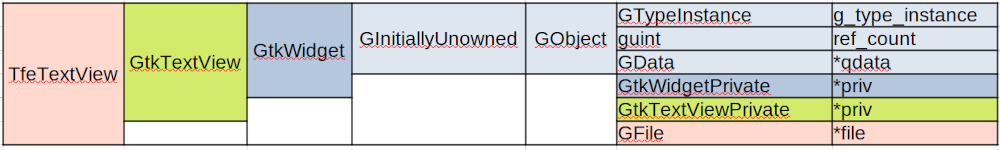
\includegraphics[width=14.39cm,height=2.16cm]{../image/TfeTextView.png}
\caption{The structure of the instance TfeTextView}
\end{figure}

Derivable classes (ancestor classes) have their own private data area
which are not included by the structure above. For example, GtkWidget
has GtkWidgetPrivate (C structure) for its private data.

Notice declarations are not definitions. So, no memories are allocated
when C structures are declared. Memories are allocated to them from the
heap area when the \passthrough{\lstinline!tfe\_text\_view\_new!}
function is called. At the same time, the ancestors' private area
allocated for the TfeTetView. They are hidden from TfeTextView and it
can't access to them directly. The created memory is called instance.
When a TfeTextView instance is created, it is given three data area.

\begin{itemize}
\tightlist
\item
  The instance (C structure).
\item
  GtkWidgetPrivate structure.
\item
  GtkTextViewPrivate structure.
\end{itemize}

TfeTextView functions can access to its instance only. The
GtkWidgetPrivate and GtkTextViewPrivate are used by the ancestors'
functions. See the following example.

\begin{lstlisting}[language=C]
GtkWidget *tv = tfe_text_view_new ();
GtkTextBuffer *buffer = gtk_text_view_get_buffer (GTK_TEXT_VIEW (tv));
\end{lstlisting}

The parent's function
\passthrough{\lstinline!gtk\_text\_view\_get\_buffer!} accesses the
GtkTextViewPrivate data (owned by \passthrough{\lstinline!tv!}). There
is a pointer, which points the GtkBuffer, in the private area and the
function returns the pointer. (Actual behavior is a bit more
complicated.)

TfeTextView instances inherit the ancestors functions like this.

A TfeTextView instance is created every time the
\passthrough{\lstinline!tfe\_text\_view\_new!} function is called.
Therefore, multiple TfeTextView instances can exist.

\subsection{Initialization of TfeTextView
instances}\label{initialization-of-tfetextview-instances}

The function \passthrough{\lstinline!tfe\_text\_view\_new!} creates a
new TfeTextView instance.

\begin{lstlisting}[language=C, numbers=left]
GtkWidget *
tfe_text_view_new (void) {
  return GTK_WIDGET (g_object_new (TFE_TYPE_TEXT_VIEW, "wrap-mode", GTK_WRAP_WORD_CHAR, NULL));
}
\end{lstlisting}

When this function is invoked, a TfeTextView instance is created and
initialized. The initialization process is as follows.

\begin{enumerate}
\def\labelenumi{\arabic{enumi}.}
\tightlist
\item
  When the instance is created, GtkWidgetPrivate and GtkTextViewPrivate
  structures are also created
\item
  Initializes GObject (GInitiallyUnowned) part in the TfeTextView
  instance.
\item
  Initializes GtkWidget part (the first \passthrough{\lstinline!priv!})
  in the TfeTextView instance and GtkWidgetPrivate structure.
\item
  Initializes GtkTextView part (the second
  \passthrough{\lstinline!priv!}) in the TfeTextView instance and
  GtkTextViewPrivate structure.
\item
  Initializes TfeTextView part (\passthrough{\lstinline!file!}) in the
  TfeTextView instance.
\end{enumerate}

The step two through four is done by
\passthrough{\lstinline!g\_object\_init!},
\passthrough{\lstinline!gtk\_widget\_init!} and
\passthrough{\lstinline!gtk\_text\_view\_init!}. They are called by the
system automatically and you don't need to care about them. Step five is
done by the function \passthrough{\lstinline!tfe\_text\_view\_init!} in
\passthrough{\lstinline!tfetextview.c!}.

\begin{lstlisting}[language=C, numbers=left]
static void
tfe_text_view_init (TfeTextView *tv) {
  tv->file = NULL;
}
\end{lstlisting}

This function just initializes \passthrough{\lstinline!tv->file!} to be
\passthrough{\lstinline!NULL!}.

\subsection{Functions and Classes}\label{functions-and-classes}

In Gtk, all objects derived from GObject have classes and instances (but
abstract objects have only classes). Instances are memory of C
structure, which are described in the previous two subsections. Each
object can have more than one instance. Those instances have the same
structure. Instances just have data. Therefore, it doesn't define
object's behavior. We need at least two things. One is functions and the
other is class methods.

The latest GTK 4 document classifies functions into a constructor,
functions and instance methods.

\begin{itemize}
\tightlist
\item
  constructors: Their name are always
  \passthrough{\lstinline!gtk\_(objectname)\_new!}. They create the
  objects.
\item
  functions: Their first parameter (argument) is \emph{NOT} the
  instance. Usually functions are utility functions for the class.
\item
  instance methods: Their first parameter (argument) is the instance.
  They do some task for the specific instance.
\end{itemize}

This tutorial uses \passthrough{\lstinline!functions!} in two ways,
broad or narrow sense.

You've already seen many functions. For example,

\begin{itemize}
\tightlist
\item
  \passthrough{\lstinline!TfeTextView *tfe\_text\_view\_new (void);!} is
  a function (constructor) to create a TfeTextView instance.
\item
  \passthrough{\lstinline!GtkTextBuffer *gtk\_text\_view\_get\_buffer (GtkTextView *textview)!}
  is a function (instance method) to get a GtkTextBuffer from
  GtkTextView.
\end{itemize}

Functions are public, which means that they are expected to be used by
other objects. They are similar to public methods in object oriented
languages.

Class (C structure) mainly consists of pointers to C functions. They are
called \emph{class methods} and used by the object itself or its
descendant objects. For example, GObject class is declared in
\passthrough{\lstinline!gobject.h!} in GLib source files.

\begin{lstlisting}[language=C, numbers=left]
typedef struct _GObjectClass             GObjectClass;
typedef struct _GObjectClass             GInitiallyUnownedClass;

struct  _GObjectClass
{
  GTypeClass   g_type_class;

  /*< private >*/
  GSList      *construct_properties;

  /*< public >*/
  /* seldom overridden */
  GObject*   (*constructor)     (GType                  type,
                                 guint                  n_construct_properties,
                                 GObjectConstructParam *construct_properties);
  /* overridable methods */
  void       (*set_property)        (GObject        *object,
                                         guint           property_id,
                                         const GValue   *value,
                                         GParamSpec     *pspec);
  void       (*get_property)        (GObject        *object,
                                         guint           property_id,
                                         GValue         *value,
                                         GParamSpec     *pspec);
  void       (*dispose)         (GObject        *object);
  void       (*finalize)        (GObject        *object);
  /* seldom overridden */
  void       (*dispatch_properties_changed) (GObject      *object,
                         guint     n_pspecs,
                         GParamSpec  **pspecs);
  /* signals */
  void       (*notify)          (GObject    *object,
                     GParamSpec *pspec);

  /* called when done constructing */
  void       (*constructed)     (GObject    *object);

  /*< private >*/
  gsize     flags;

  gsize         n_construct_properties;

  gpointer pspecs;
  gsize n_pspecs;

  /* padding */
  gpointer  pdummy[3];
};
\end{lstlisting}

There's a pointer to the function \passthrough{\lstinline!dispose!} in
line 25.

\begin{lstlisting}[language=C]
void (*dispose) (GObject *object);
\end{lstlisting}

The declaration is a bit complicated. The asterisk before the identifier
\passthrough{\lstinline!dispose!} means pointer. So, the pointer
\passthrough{\lstinline!dispose!} points to a function which has one
parameter, which points a GObject structure, and returns no value. In
the same way, line 26 says \passthrough{\lstinline!finalize!} is a
pointer to the function which has one parameter, which points a GObject
structure, and returns no value.

\begin{lstlisting}[language=C]
void (*finalize) (GObject *object);
\end{lstlisting}

Look at the declaration of \passthrough{\lstinline!\_GObjectClass!} so
that you would find that most of the members are pointers to functions.

\begin{itemize}
\tightlist
\item
  13: A function pointed by \passthrough{\lstinline!constructor!} is
  called when the instance is created. It completes the initialization
  of the instance.
\item
  25: A function pointed by \passthrough{\lstinline!dispose!} is called
  when the instance destructs itself. Destruction process is divided
  into two phases. The first one is called disposing. In this phase, the
  instance releases all the references to other instances. The second
  phase is finalizing.
\item
  26: A function pointed by \passthrough{\lstinline!finalize!} finishes
  the destruction process.
\item
  The other pointers point to functions which are called while the
  instance lives.
\end{itemize}

These functions are called class methods. The methods are open to its
descendants. But not open to the objects which are not the descendants.

\subsection{TfeTextView class}\label{tfetextview-class}

TfeTextView class is a structure and it includes all its ancestors'
classes in it. Therefore, classes have similar hierarchy to instances.

\begin{lstlisting}
GObjectClass (GInitiallyUnownedClass) -- GtkWidgetClass -- GtkTextViewClass -- TfeTextViewClass
\end{lstlisting}

The following is extracted from the source codes (not exactly the same).

\begin{lstlisting}[language=C, numbers=left]
struct _GtkWidgetClass
{
  GInitiallyUnownedClass parent_class;

  /*< public >*/

  /* basics */
  void (* show)                (GtkWidget        *widget);
  void (* hide)                (GtkWidget        *widget);
  void (* map)                 (GtkWidget        *widget);
  void (* unmap)               (GtkWidget        *widget);
  void (* realize)             (GtkWidget        *widget);
  void (* unrealize)           (GtkWidget        *widget);
  void (* root)                (GtkWidget        *widget);
  void (* unroot)              (GtkWidget        *widget);
  void (* size_allocate)       (GtkWidget           *widget,
                                int                  width,
                                int                  height,
                                int                  baseline);
  void (* state_flags_changed) (GtkWidget        *widget,
                                GtkStateFlags     previous_state_flags);
  void (* direction_changed)   (GtkWidget        *widget,
                                GtkTextDirection  previous_direction);

  /* size requests */
  GtkSizeRequestMode (* get_request_mode)               (GtkWidget      *widget);
  void              (* measure) (GtkWidget      *widget,
                                 GtkOrientation  orientation,
                                 int             for_size,
                                 int            *minimum,
                                 int            *natural,
                                 int            *minimum_baseline,
                                 int            *natural_baseline);

  /* Mnemonics */
  gboolean (* mnemonic_activate)        (GtkWidget           *widget,
                                         gboolean             group_cycling);

  /* explicit focus */
  gboolean (* grab_focus)               (GtkWidget           *widget);
  gboolean (* focus)                    (GtkWidget           *widget,
                                         GtkDirectionType     direction);
  void     (* set_focus_child)          (GtkWidget           *widget,
                                         GtkWidget           *child);

  /* keyboard navigation */
  void     (* move_focus)               (GtkWidget           *widget,
                                         GtkDirectionType     direction);
  gboolean (* keynav_failed)            (GtkWidget           *widget,
                                         GtkDirectionType     direction);

  gboolean     (* query_tooltip)      (GtkWidget  *widget,
                                       int         x,
                                       int         y,
                                       gboolean    keyboard_tooltip,
                                       GtkTooltip *tooltip);

  void         (* compute_expand)     (GtkWidget  *widget,
                                       gboolean   *hexpand_p,
                                       gboolean   *vexpand_p);

  void         (* css_changed)                 (GtkWidget            *widget,
                                                GtkCssStyleChange    *change);

  void         (* system_setting_changed)      (GtkWidget            *widget,
                                                GtkSystemSetting      settings);

  void         (* snapshot)                    (GtkWidget            *widget,
                                                GtkSnapshot          *snapshot);

  gboolean     (* contains)                    (GtkWidget *widget,
                                                double     x,
                                                double     y);

  /*< private >*/

  GtkWidgetClassPrivate *priv;

  gpointer padding[8];
};

struct _GtkTextViewClass
{
  GtkWidgetClass parent_class;

  /*< public >*/

  void (* move_cursor)           (GtkTextView      *text_view,
                                  GtkMovementStep   step,
                                  int               count,
                                  gboolean          extend_selection);
  void (* set_anchor)            (GtkTextView      *text_view);
  void (* insert_at_cursor)      (GtkTextView      *text_view,
                                  const char       *str);
  void (* delete_from_cursor)    (GtkTextView      *text_view,
                                  GtkDeleteType     type,
                                  int               count);
  void (* backspace)             (GtkTextView      *text_view);
  void (* cut_clipboard)         (GtkTextView      *text_view);
  void (* copy_clipboard)        (GtkTextView      *text_view);
  void (* paste_clipboard)       (GtkTextView      *text_view);
  void (* toggle_overwrite)      (GtkTextView      *text_view);
  GtkTextBuffer * (* create_buffer) (GtkTextView   *text_view);
  void (* snapshot_layer)        (GtkTextView      *text_view,
                      GtkTextViewLayer  layer,
                      GtkSnapshot      *snapshot);
  gboolean (* extend_selection)  (GtkTextView            *text_view,
                                  GtkTextExtendSelection  granularity,
                                  const GtkTextIter      *location,
                                  GtkTextIter            *start,
                                  GtkTextIter            *end);
  void (* insert_emoji)          (GtkTextView      *text_view);

  /*< private >*/

  gpointer padding[8];
};

/* The following definition is generated by the macro G_DECLARE_FINAL_TYPE */
typedef struct {
  GtkTextView parent_class;
} TfeTextViewClass;
\end{lstlisting}

\begin{itemize}
\tightlist
\item
  120-122: This three lines are generated by the macro
  \passthrough{\lstinline!G\_DECLARE\_FINAL\_TYPE!}. So, they are not
  written in either \passthrough{\lstinline!tfe\_text\_view.h!} or
  \passthrough{\lstinline!tfe\_text\_view.c!}.
\item
  3, 84, 121: Each class has its parent class at the first member of its
  structure. It is the same as instance structures.
\item
  Class members in ancestors are open to the descendant class. So, they
  can be changed in
  \passthrough{\lstinline!tfe\_text\_view\_class\_init!} function. For
  example, the \passthrough{\lstinline!dispose!} pointer in GObjectClass
  will be overridden later in
  \passthrough{\lstinline!tfe\_text\_view\_class\_init!}. (Override is
  an object oriented programming terminology. Override is rewriting
  ancestors' class methods in the descendant class.)
\item
  Some class methods are often overridden.
  \passthrough{\lstinline!set\_property!},
  \passthrough{\lstinline!get\_property!},
  \passthrough{\lstinline!dispose!}, \passthrough{\lstinline!finalize!}
  and \passthrough{\lstinline!constructed!} are such methods.
\end{itemize}

TfeTextViewClass includes its ancestors' class in it. It is illustrated
in the following diagram.

\begin{figure}
\centering
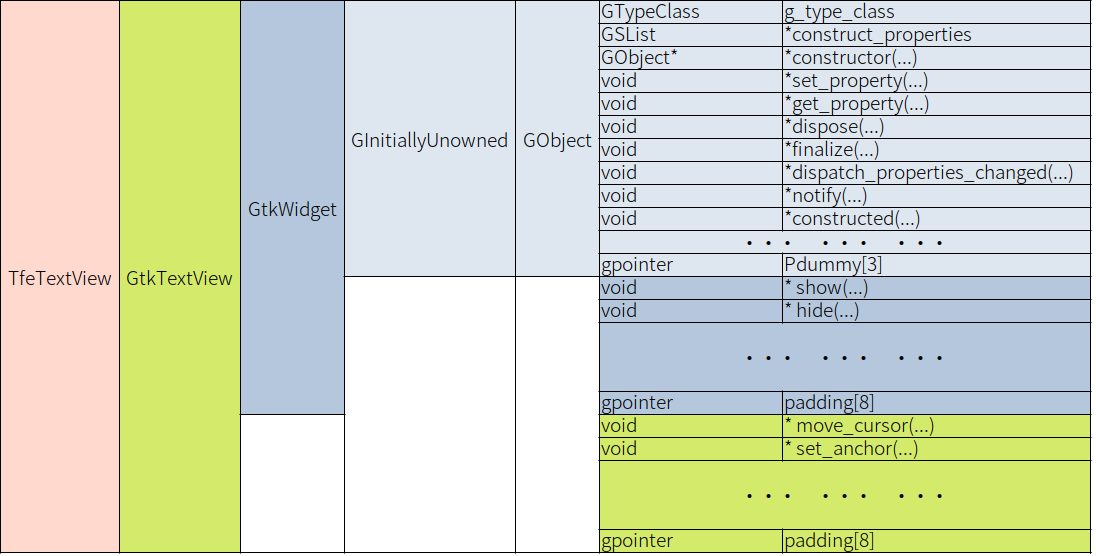
\includegraphics[width=16.02cm,height=8.34cm]{../image/TfeTextViewClass.png}
\caption{The structure of TfeTextView Class}
\end{figure}

\subsection{Destruction of
TfeTextView}\label{destruction-of-tfetextview}

Every Object derived from GObject has a reference count. If an object A
refers to an object B, then A keeps a pointer to B in A and at the same
time increases the reference count of B by one with the function
\passthrough{\lstinline!g\_object\_ref (B)!}. If A doesn't need B any
longer, A discards the pointer to B (usually it is done by assigning
NULL to the pointer) and decreases the reference count of B by one with
the function \passthrough{\lstinline!g\_object\_unref (B)!}.

If two objects A and B refer to C, then the reference count of C is two.
If A no longer needs C, A discards the pointer to C and decreases the
reference count in C by one. Now the reference count of C is one. In the
same way, if B no longer needs C, B discards the pointer to C and
decreases the reference count in C by one. At this moment, no object
refers to C and the reference count of C is zero. This means C is no
longer useful. Then C destructs itself and finally the memories
allocated to C is freed.

\begin{figure}
\centering
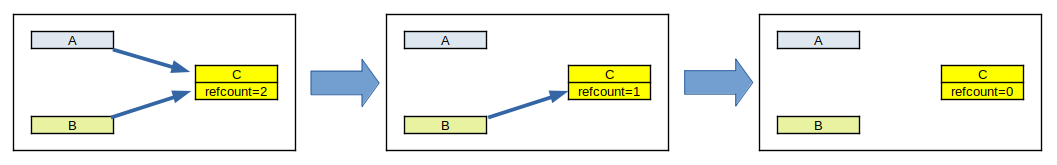
\includegraphics[width=15.855cm,height=2.475cm]{../image/refcount.png}
\caption{Reference count of B}
\end{figure}

The idea above is based on an assumption that an object referred by
nothing has reference count of zero. When the reference count drops to
zero, the object starts its destruction process. The destruction process
is split into two phases: disposing and finalizing. In the disposing
process, the object invokes the function pointed by
\passthrough{\lstinline!dispose!} in its class to release all references
to other instances. After that, it invokes the function pointed by
\passthrough{\lstinline!finalize!} in its class to complete the
destruction process.

In the destruction process, TfeTextView needs to unref the GFile pointed
by \passthrough{\lstinline!tv->file!}. You must write the dispose
handler \passthrough{\lstinline!tfe\_text\_view\_dispose!}.

\begin{lstlisting}[language=C, numbers=left]
static void
tfe_text_view_dispose (GObject *gobject) {
  TfeTextView *tv = TFE_TEXT_VIEW (gobject);

  if (G_IS_FILE (tv->file))
    g_clear_object (&tv->file);

  G_OBJECT_CLASS (tfe_text_view_parent_class)->dispose (gobject);
}
\end{lstlisting}

\begin{itemize}
\tightlist
\item
  5,6: If \passthrough{\lstinline!tv->file!} points a GFile, it
  decreases the reference count of the GFile instance. The function
  \passthrough{\lstinline!g\_clear\_object!} decreases the reference
  count and assigns NULL to \passthrough{\lstinline!tv->file!}. In
  dispose handlers, we usually use
  \passthrough{\lstinline!g\_clear\_object!} rather than
  \passthrough{\lstinline!g\_object\_unref!}.
\item
  8: invokes parent's dispose handler. (This will be explained later.)
\end{itemize}

In the disposing process, the object uses the pointer in its class to
call the handler. Therefore,
\passthrough{\lstinline!tfe\_text\_view\_dispose!} needs to be
registered in the class when the TfeTextView class is initialized. The
function \passthrough{\lstinline!tfe\_text\_view\_class\_init!} is the
class initialization function and it is declared in the
\passthrough{\lstinline!G\_DEFINE\_TYPE!} macro expansion.

\begin{lstlisting}[language=C]
static void
tfe_text_view_class_init (TfeTextViewClass *class) {
  GObjectClass *object_class = G_OBJECT_CLASS (class);

  object_class->dispose = tfe_text_view_dispose;
}
\end{lstlisting}

Each ancestors' class has been created before TfeTextViewClass is
created. Therefore, there are four classes and each class has a pointer
to each dispose handler. Look at the following diagram. There are four
classes -- GObjectClass (GInitiallyUnownedClass), GtkWidgetClass,
GtkTextViewClass and TfeTextViewClass. Each class has its own dispose
handler -- \passthrough{\lstinline!dh1!}, \passthrough{\lstinline!dh2!},
\passthrough{\lstinline!dh3!} and
\passthrough{\lstinline!tfe\_text\_view\_dispose!}.

\begin{figure}
\centering
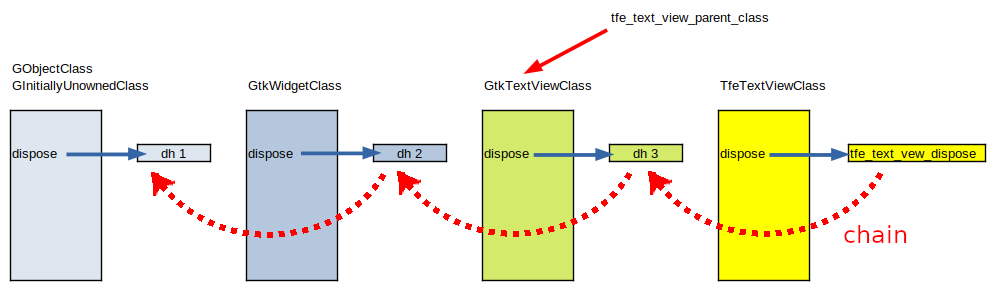
\includegraphics[width=14.925cm,height=4.455cm]{../image/dispose_handler.png}
\caption{dispose handlers}
\end{figure}

Now, look at the \passthrough{\lstinline!tfe\_text\_view\_dispose!}
program above. It first releases the reference to GFile object pointed
by \passthrough{\lstinline!tv->file!}. Then it invokes its parent's
dispose handler in line 8.

\begin{lstlisting}[language=C]
G_OBJECT_CLASS (tfe_text_view_parent_class)->dispose (gobject);
\end{lstlisting}

A variable \passthrough{\lstinline!tfe\_text\_view\_parent\_class!},
which is made by \passthrough{\lstinline!G\_DEFINE\_FINAL\_TYPE!} macro,
is a pointer that points the parent object class. The variable
\passthrough{\lstinline!gobject!} is a pointer to TfeTextView instance
which is casted as a GObject instance. Therefore,
\passthrough{\lstinline!G\_OBJECT\_CLASS (tfe\_text\_view\_parent\_class)->dispose!}
points the handler \passthrough{\lstinline!dh3!} in the diagram above.
The statement
\passthrough{\lstinline!G\_OBJECT\_CLASS (tfe\_text\_view\_parent\_class)->dispose (gobject)!}
is the same as \passthrough{\lstinline!dh3 (gobject)!}, which means it
releases all the reference to the other instances in the
GtkTextViewPrivate in the TfeTextView instance. After that,
\passthrough{\lstinline!dh3!} calls \passthrough{\lstinline!dh2!}, and
\passthrough{\lstinline!dh2!} calls \passthrough{\lstinline!dh1!}.
Finally all the references are released.

  \section{Signals}\label{signals}

\subsection{Signals}\label{signals-1}

Each object is encapsulated in Gtk programming. And it is not
recommended to use global variables because they are prone to make the
program complicated. So, we need something to communicate between
objects. There are two ways to do so.

\begin{itemize}
\tightlist
\item
  Instance methods: Instance methods are functions on instances. For
  example,
  \passthrough{\lstinline!tb = gtk\_text\_view\_get\_buffer (tv)!} is an
  instance method on the instance \passthrough{\lstinline!tv!}. The
  caller requests \passthrough{\lstinline!tv!} to give
  \passthrough{\lstinline!tb!}, which is a GtkTextBuffer instance
  connected to \passthrough{\lstinline!tv!}.
\item
  Signals: For example, \passthrough{\lstinline!activate!} signal on
  GApplication object. When the application is activated, the signal is
  emitted. Then the handler, which has been connected to the signal, is
  invoked.
\end{itemize}

The caller of methods or signals are usually out of the object. One of
the difference between these two is that the object is active or
passive. In methods, objects passively respond to the caller. In
signals, objects actively send signals to handlers.

GObject signals are registered, connected and emitted.

\begin{enumerate}
\def\labelenumi{\arabic{enumi}.}
\tightlist
\item
  Signals are registered in the class. The registration is done usually
  when the class is initialized. Signals can have a default handler,
  which is sometimes called ``object method handler''. It is not a user
  handler connected by \passthrough{\lstinline!g\_signal\_connect!}
  family functions. A default handler is always called on any instance
  of the class.
\item
  Signals are connected to handlers by the macro
  \passthrough{\lstinline!g\_signal\_connect!} or its family functions.
  The connection is usually done out of the object. One important thing
  is that signals are connected on a certain instance. Suppose there
  exist two GtkButton instances A, B and a function C. Even if you
  connected the ``clicked'' signal on A to C, B and C are \emph{not}
  connected.
\item
  When Signals are emitted, the connected handlers are invoked. Signals
  are emitted on the instance of the class.
\end{enumerate}

\subsection{Signal registration}\label{signal-registration}

In TfeTextView, two signals are registered.

\begin{itemize}
\tightlist
\item
  ``change-file'' signal. This signal is emitted when
  \passthrough{\lstinline!tv->file!} is changed.
\item
  ``open-response'' signal. The function
  \passthrough{\lstinline!tfe\_text\_view\_open!} doesn't return the
  status because it can't get the status from the file chooser dialog.
  (Instead, the call back function gets the status.) This signal is
  emitted instead of the return value of the function.
\end{itemize}

A static variable or array is used to store signal ID.

\begin{lstlisting}[language=C]
enum {
  CHANGE_FILE,
  OPEN_RESPONSE,
  NUMBER_OF_SIGNALS
};

static guint tfe_text_view_signals[NUMBER_OF_SIGNALS];
\end{lstlisting}

Signals are registered in the class initialization function.

\begin{lstlisting}[language=C, numbers=left]
static void
tfe_text_view_class_init (TfeTextViewClass *class) {
  GObjectClass *object_class = G_OBJECT_CLASS (class);

  object_class->dispose = tfe_text_view_dispose;
  tfe_text_view_signals[CHANGE_FILE] = g_signal_new ("change-file",
                                 G_TYPE_FROM_CLASS (class),
                                 G_SIGNAL_RUN_LAST | G_SIGNAL_NO_RECURSE | G_SIGNAL_NO_HOOKS,
                                 0 /* class offset */,
                                 NULL /* accumulator */,
                                 NULL /* accumulator data */,
                                 NULL /* C marshaller */,
                                 G_TYPE_NONE /* return_type */,
                                 0     /* n_params */
                                 );
  tfe_text_view_signals[OPEN_RESPONSE] = g_signal_new ("open-response",
                                 G_TYPE_FROM_CLASS (class),
                                 G_SIGNAL_RUN_LAST | G_SIGNAL_NO_RECURSE | G_SIGNAL_NO_HOOKS,
                                 0 /* class offset */,
                                 NULL /* accumulator */,
                                 NULL /* accumulator data */,
                                 NULL /* C marshaller */,
                                 G_TYPE_NONE /* return_type */,
                                 1     /* n_params */,
                                 G_TYPE_INT
                                 );
}
\end{lstlisting}

\begin{itemize}
\tightlist
\item
  6-15: Registers ``change-file'' signal.
  \passthrough{\lstinline!g\_signal\_new!} function is used. The signal
  ``change-file'' has no default handler (object method handler) so the
  offset (the line 9) is set to zero. You usually don't need a default
  handler. If you need it, use
  \passthrough{\lstinline!g\_signal\_new\_class\_handler!} function
  instead of \passthrough{\lstinline!g\_signal\_new!}. See
  \href{https://docs.gtk.org/gobject/func.signal_new_class_handler.html}{GObject
  API Reference} for further information.
\item
  The return value of \passthrough{\lstinline!g\_signal\_new!} is the
  signal id. The type of signal id is guint, which is the same as
  unsigned int. It is used in the function
  \passthrough{\lstinline!g\_signal\_emit!}.
\item
  16-26: Registers ``open-response'' signal. This signal has a
  parameter.
\item
  24: Number of the parameters. ``open-response'' signal has one
  parameter.
\item
  25: The type of the parameter. \passthrough{\lstinline!G\_TYPE\_INT!}
  is a type of integer. Such fundamental types are described in
  \href{https://developer-old.gnome.org/gobject/stable/gobject-Type-Information.html}{GObject
  reference manual}.
\end{itemize}

The handlers are declared as follows.

\begin{lstlisting}[language=C]
/* "change-file" signal handler */
void
user_function (TfeTextView *tv,
               gpointer user_data)

/* "open-response" signal handler */
void
user_function (TfeTextView *tv,
               TfeTextViewOpenResponseType response-id,
               gpointer user_data)
\end{lstlisting}

\begin{itemize}
\tightlist
\item
  The signal ``change-file'' doesn't have parameter, so the handler's
  arguments are a TfeTextView instance and a user data.
\item
  The signal ``open-response'' signal has one parameter and its
  arguments are a TfeTextView instance, the signal's parameter and user
  data.
\item
  The variable \passthrough{\lstinline!tv!} points the instance on which
  the signal is emitted.
\item
  The last argument \passthrough{\lstinline!user\_data!} comes from the
  fourth argument of \passthrough{\lstinline!g\_signal\_connect!}.
\item
  The \passthrough{\lstinline!parameter!}
  (\passthrough{\lstinline!response-id!}) comes from the fourth argument
  of \passthrough{\lstinline!g\_signal\_emit!}.
\end{itemize}

The values of the type
\passthrough{\lstinline!TfeTextViewOpenResponseType!} are defined in
\passthrough{\lstinline!tfetextview.h!}.

\begin{lstlisting}[language=C]
/* "open-response" signal response */
enum TfeTextViewOpenResponseType
{
  TFE_OPEN_RESPONSE_SUCCESS,
  TFE_OPEN_RESPONSE_CANCEL,
  TFE_OPEN_RESPONSE_ERROR
};
\end{lstlisting}

\begin{itemize}
\tightlist
\item
  The parameter is set to
  \passthrough{\lstinline!TFE\_OPEN\_RESPONSE\_SUCCESS!} when
  \passthrough{\lstinline!tfe\_text\_view\_open!} has successfully
  opened a file and read it.
\item
  The parameter is set to
  \passthrough{\lstinline!TFE\_OPEN\_RESPONSE\_CANCEL!} when the user
  has canceled.
\item
  The parameter is set to
  \passthrough{\lstinline!TFE\_OPEN\_RESPONSE\_ERROR!} when an error has
  occurred.
\end{itemize}

\subsection{Signal connection}\label{signal-connection}

A signal and a handler are connected by the function macro
\passthrough{\lstinline!g\_signal\_connect!}. There are some similar
function macros like
\passthrough{\lstinline!g\_signal\_connect\_after!},
\passthrough{\lstinline!g\_signal\_connect\_swapped!} and so on.
However, \passthrough{\lstinline!g\_signal\_connect!} is used most
often. The signals ``change-file'' and ``open-response'' are connected
to their callback functions out of the TfeTextView object. Those
callback functions are defined by users.

For example, callback functions are defined in
\passthrough{\lstinline!src/tfe6/tfewindow.c!} and their names are
\passthrough{\lstinline!file\_changed\_cb!} and
\passthrough{\lstinline!open\_response\_cb!}. They will be explained
later.

\begin{lstlisting}[language=C]
g_signal_connect (GTK_TEXT_VIEW (tv), "change-file", G_CALLBACK (file_changed_cb), nb);

g_signal_connect (TFE_TEXT_VIEW (tv), "open-response", G_CALLBACK (open_response_cb), nb);
\end{lstlisting}

\subsection{Signal emission}\label{signal-emission}

A signal is emitted on the instance. A function
\passthrough{\lstinline!g\_signal\_emit!} is used to emit the signal.
The following lines are extracted from
\passthrough{\lstinline!src/tfetextview/tfetextview.c!}. Each line comes
from a different line.

\begin{lstlisting}[language=C]
g_signal_emit (tv, tfe_text_view_signals[CHANGE_FILE], 0);
g_signal_emit (tv, tfe_text_view_signals[OPEN_RESPONSE], 0, TFE_OPEN_RESPONSE_SUCCESS);
g_signal_emit (tv, tfe_text_view_signals[OPEN_RESPONSE], 0, TFE_OPEN_RESPONSE_CANCEL);
g_signal_emit (tv, tfe_text_view_signals[OPEN_RESPONSE], 0, TFE_OPEN_RESPONSE_ERROR);
\end{lstlisting}

\begin{itemize}
\tightlist
\item
  The first argument is the instance on which the signal is emitted.
\item
  The second argument is the signal id.
\item
  The third argument is the detail of the signal. The signals
  ``change-file'' and ``open-response'' don't have details and the
  arguments are zero.
\item
  The signal ``change-file'' doesn't have parameters, so there's no
  fourth argument.
\item
  The signal ``open-response'' has one parameter. The fourth argument is
  the parameter.
\end{itemize}

  \section{TfeTextView class}\label{tfetextview-class}

The TfeTextView class will be finally completed in this section. The
remaining topic is functions. TfeTextView functions, which are
constructors and instance methods, are described in this section.

The source files are in the directory
\passthrough{\lstinline!src/tfetextview!}. You can get them by
downloading the
\href{https://github.com/ToshioCP/Gtk4-tutorial}{repository}.

\subsection{tfetextview.h}\label{tfetextview.h}

The header file \passthrough{\lstinline!tfetextview.h!} provides:

\begin{itemize}
\tightlist
\item
  The type of TfeTextView, which is
  \passthrough{\lstinline!TFE\_TYPE\_TEXT\_VIEW!}.
\item
  The macro \passthrough{\lstinline!G\_DECLARE\_FINAL\_TYPE!}, the
  expansion of which includes some useful functions and definitions.
\item
  Constants for the \passthrough{\lstinline!open-response!} signal.
\item
  Public functions of \passthrough{\lstinline!tfetextview.c!}. They are
  constructors and instance methods.
\end{itemize}

Therefore, Any programs use TfeTextView needs to include
\passthrough{\lstinline!tfetextview.h!}.

\begin{lstlisting}[language=C, numbers=left]
#pragma once

#include <gtk/gtk.h>

#define TFE_TYPE_TEXT_VIEW tfe_text_view_get_type ()
G_DECLARE_FINAL_TYPE (TfeTextView, tfe_text_view, TFE, TEXT_VIEW, GtkTextView)

/* "open-response" signal response */
enum TfeTextViewOpenResponseType
{
  TFE_OPEN_RESPONSE_SUCCESS,
  TFE_OPEN_RESPONSE_CANCEL,
  TFE_OPEN_RESPONSE_ERROR
};

GFile *
tfe_text_view_get_file (TfeTextView *tv);

void
tfe_text_view_open (TfeTextView *tv, GtkWindow *win);

void
tfe_text_view_save (TfeTextView *tv);

void
tfe_text_view_saveas (TfeTextView *tv);

GtkWidget *
tfe_text_view_new_with_file (GFile *file);

GtkWidget *
tfe_text_view_new (void);
\end{lstlisting}

\begin{itemize}
\tightlist
\item
  1: The preprocessor directive \passthrough{\lstinline!\#pragma once!}
  makes the header file be included only once. It is non-standard but
  widely used.
\item
  3: Includes gtk4 header files. The header file
  \passthrough{\lstinline!gtk4!} also has the same mechanism to avoid
  being included multiple times.
\item
  5-6: These two lines define TfeTextView type, its class structure and
  some useful definitions.

  \begin{itemize}
  \tightlist
  \item
    \passthrough{\lstinline!TfeTextView!} and
    \passthrough{\lstinline!TfeTextViewClass!} are declared as typedef
    of C structures.
  \item
    You need to define a structure
    \passthrough{\lstinline!\_TfeTextView!} later.
  \item
    The class structure \passthrough{\lstinline!\_TfeTextViewClass!} is
    defined here. You don't need to define it by yourself.
  \item
    Convenience functions \passthrough{\lstinline!TFE\_TEXT\_VIEW ()!}
    for casting and \passthrough{\lstinline!TFE\_IS\_TEXT\_VIEW!} for
    type check are defined.
  \end{itemize}
\item
  8-14: A definition of the values of the ``open-response'' signal
  parameters.
\item
  16-32: Declarations of public functions on TfeTextView.
\end{itemize}

\subsection{Constructors}\label{constructors}

A TfeTextView instance is created with
\passthrough{\lstinline!tfe\_text\_view\_new!} or
\passthrough{\lstinline!tfe\_text\_view\_new\_with\_file!}. These
functions are called constructors.

\begin{lstlisting}[language=C]
GtkWidget *tfe_text_view_new (void);
\end{lstlisting}

It just creates a new TfeTextView instance and returns the pointer to
the new instance.

\begin{lstlisting}[language=C]
GtkWidget *tfe_text_view_new_with_file (GFile *file);
\end{lstlisting}

It is given a Gfile object as an argument and it loads the file into the
GtkTextBuffer instance, then returns the pointer to the new instance.
The argument \passthrough{\lstinline!file!} is owned by the caller and
the function doesn't change it. If an error occurs during the creation
process, NULL will be returned.

Each function is defined as follows.

\begin{lstlisting}[language=C, numbers=left]
GtkWidget *
tfe_text_view_new_with_file (GFile *file) {
  g_return_val_if_fail (G_IS_FILE (file), NULL);

  GtkWidget *tv;
  GtkTextBuffer *tb;
  char *contents;
  gsize length;

  if (! g_file_load_contents (file, NULL, &contents, &length, NULL, NULL)) /* read error */
    return NULL;

  tv = tfe_text_view_new();
  tb = gtk_text_view_get_buffer (GTK_TEXT_VIEW (tv));
  gtk_text_buffer_set_text (tb, contents, length);
  TFE_TEXT_VIEW (tv)->file = g_file_dup (file);
  gtk_text_buffer_set_modified (tb, FALSE);
  g_free (contents);
  return tv;
}

GtkWidget *
tfe_text_view_new (void) {
  return GTK_WIDGET (g_object_new (TFE_TYPE_TEXT_VIEW, "wrap-mode", GTK_WRAP_WORD_CHAR, NULL));
}
\end{lstlisting}

\begin{itemize}
\tightlist
\item
  22-25: \passthrough{\lstinline!tfe\_text\_view\_new!} function. Just
  returns the value from the function
  \passthrough{\lstinline!g\_object\_new!} but casts it to the pointer
  to GtkWidget. The function \passthrough{\lstinline!g\_object\_new!}
  creates any instances of its descendant class. The arguments are the
  type of the class, property list and NULL, which is the end mark of
  the property list. TfeTextView ``wrap-mode'' property has
  GTK\_WRAP\_WORD\_CHAR as the default value.
\item
  1-20: \passthrough{\lstinline!tfe\_text\_view\_new\_with\_file!}
  function.
\item
  3: \passthrough{\lstinline!g\_return\_val\_if\_fail!} is described in
  \href{https://docs.gtk.org/glib/func.return_val_if_fail.html}{GLib API
  Reference -- g\_return\_val\_if\_fail}. And also
  \href{https://docs.gtk.org/glib/logging.html}{GLib API Reference --
  Message Logging}. It tests whether the argument
  \passthrough{\lstinline!file!} is a pointer to GFile. If it's true,
  the program goes on to the next line. If it's false, it returns NULL
  (the second argument) immediately. And at the same time it logs out
  the error message (usually the log is outputted to stderr or stdout).
  This function is used to check the programmer's error. If an error
  occurs, the solution is usually to change the (caller) program and fix
  the bug. You need to distinguish programmer's errors and runtime
  errors. You shouldn't use this function to find runtime errors.
\item
  10-11: Reads the file. If an error occurs, NULL is returned.
\item
  13: Calls the function \passthrough{\lstinline!tfe\_text\_view\_new!}.
  The function creates TfeTextView instance and returns the pointer to
  the instance.
\item
  14: Gets the pointer to the GtkTextBuffer instance corresponds to
  \passthrough{\lstinline!tv!}. The pointer is assigned to
  \passthrough{\lstinline!tb!}
\item
  15: Assigns the contents read from the file to
  \passthrough{\lstinline!tb!}.
\item
  16: Duplicates \passthrough{\lstinline!file!} and sets
  \passthrough{\lstinline!tv->file!} to point it. GFile is \emph{not}
  thread safe. The duplication makes sure that the GFile instance of
  \passthrough{\lstinline!tv!} keeps the file information even if the
  original one is changed by other thread.
\item
  17: The function
  \passthrough{\lstinline!gtk\_text\_buffer\_set\_modified (tb, FALSE)!}
  sets the modification flag of \passthrough{\lstinline!tb!} to FALSE.
  The modification flag indicates that the contents has been modified.
  It is used when the contents are saved. If the modification flag is
  FALSE, it doesn't need to save the contents.
\item
  18: Frees the memories pointed by \passthrough{\lstinline!contents!}.
\item
  19: Returns \passthrough{\lstinline!tv!}, which is a pointer to the
  newly created TfeTextView instance. If an error happens, NULL is
  returned.
\end{itemize}

\subsection{Save and saveas functions}\label{save-and-saveas-functions}

Save and saveas functions write the contents in the GtkTextBuffer to a
file.

\begin{lstlisting}[language=C]
void tfe_text_view_save (TfeTextView *tv)
\end{lstlisting}

The function \passthrough{\lstinline!tfe\_text\_view\_save!} writes the
contents in the GtkTextBuffer to a file specified by
\passthrough{\lstinline!tv->file!}. If
\passthrough{\lstinline!tv->file!} is NULL, then it shows file chooser
dialog and prompts the user to choose a file to save. Then it saves the
contents to the file and sets \passthrough{\lstinline!tv->file!} to
point the GFile instance for the file.

\begin{lstlisting}[language=C]
void tfe_text_view_saveas (TfeTextView *tv)
\end{lstlisting}

The function \passthrough{\lstinline!saveas!} shows a file chooser
dialog and prompts the user to select a existed file or specify a new
file to save. Then, the function changes
\passthrough{\lstinline!tv->file!} and save the contents to the
specified file. If an error occurs, it is shown to the user through the
alert dialog. The error is managed only in the TfeTextView and no
information is notified to the caller.

\subsubsection{save\_file function}\label{save_file-function}

\begin{lstlisting}[language=C, numbers=left]
static gboolean
save_file (GFile *file, GtkTextBuffer *tb, GtkWindow *win) {
  GtkTextIter start_iter;
  GtkTextIter end_iter;
  char *contents;
  gboolean stat;
  GtkAlertDialog *alert_dialog;
  GError *err = NULL;

  gtk_text_buffer_get_bounds (tb, &start_iter, &end_iter);
  contents = gtk_text_buffer_get_text (tb, &start_iter, &end_iter, FALSE);
  stat = g_file_replace_contents (file, contents, strlen (contents), NULL, TRUE, G_FILE_CREATE_NONE, NULL, NULL, &err);
  if (stat)
    gtk_text_buffer_set_modified (tb, FALSE);
  else {
    alert_dialog = gtk_alert_dialog_new ("%s", err->message);
    gtk_alert_dialog_show (alert_dialog, win);
    g_object_unref (alert_dialog);
    g_error_free (err);
  }
  g_free (contents);
  return stat;
}
\end{lstlisting}

\begin{itemize}
\tightlist
\item
  The function \passthrough{\lstinline!save\_file!} is called from
  \passthrough{\lstinline!saveas\_dialog\_response!} and
  \passthrough{\lstinline!tfe\_text\_view\_save!}. This function saves
  the contents of the buffer to the file given as an argument. If error
  happens, it displays an error message. So, a caller of this function
  don't need to take care of errors. The class of this function is
  \passthrough{\lstinline!static!}. Therefore, only functions in this
  file (\passthrough{\lstinline!tfetextview.c!}) call this function.
  Such static functions usually don't have
  \passthrough{\lstinline!g\_return\_val\_if\_fail!} functions.
\item
  10-11: Gets the text contents from the buffer.
\item
  12: The function \passthrough{\lstinline!g\_file\_replace\_contents!}
  writes the contents to the file and returns the status (true =
  success/ false = fail). It has many parameters, but some of them are
  almost always given the same values.

  \begin{itemize}
  \tightlist
  \item
    GFile* file: GFile to which the contents are saved.
  \item
    const char* contents: contents to be saved. The string is owned by
    the caller.
  \item
    gsize length: the length of the contents
  \item
    const char* etag: entity tag. It is usually NULL.
  \item
    gboolean make\_backup: true to make a backup if the file exists.
    false not to make it. the file will be overwritten.
  \item
    GFileCreateFlags flags: usually
    \passthrough{\lstinline!G\_FILE\_CREATE\_NONE!} is fine.
  \item
    char** new\_etag: new entity tag. It is usually NULL.
  \item
    GCancellable* cancellable: If a cancellable instance is set, the
    other thread can cancel this operation. it is usually NULL.
  \item
    GError** error: If error happens, GError will be set.
  \end{itemize}
\item
  13,14: If no error happens, set the modified flag to be FALSE. This
  means that the buffer is not modified since it has been saved.
\item
  16-19: If it fails to save the contents, an error message will be
  displayed.
\item
  16: Creates an alert dialog. The parameters are printf-like format
  string followed by values to insert into the string. GtkAlertDialog is
  available since version 4.10. If your version is older than 4.10, use
  GtkMessageDialog instead. GtkMessageDialog is deprecated since version
  4.10.
\item
  17: Show the alert dialog. The parameters are the dialog and the
  transient parent window. This allows window managers to keep the
  dialog on top of the parent window, or center the dialog over the
  parent window. It is possible to give no parent window to the dialog
  by giving NULL as the argument. However, it is encouraged to give
  parents to dialogs.
\item
  18: Releases the dialog.
\item
  19: Frees the GError struct pointed by \passthrough{\lstinline!err!}
  with \passthrough{\lstinline!g\_error\_free!} function.
\item
  21: Frees \passthrough{\lstinline!contents!}.
\item
  22: Returns the status to the caller.
\end{itemize}

\subsubsection{save\_dialog\_cb function}\label{save_dialog_cb-function}

\begin{lstlisting}[language=C, numbers=left]
static void
save_dialog_cb(GObject *source_object, GAsyncResult *res, gpointer data) {
  GtkFileDialog *dialog = GTK_FILE_DIALOG (source_object);
  TfeTextView *tv = TFE_TEXT_VIEW (data);
  GtkTextBuffer *tb = gtk_text_view_get_buffer (GTK_TEXT_VIEW (tv));
  GFile *file;
  GtkWidget *win = gtk_widget_get_ancestor (GTK_WIDGET (tv), GTK_TYPE_WINDOW);
  GError *err = NULL;
  GtkAlertDialog *alert_dialog;

  if (((file = gtk_file_dialog_save_finish (dialog, res, &err)) != NULL) && save_file(file, tb, GTK_WINDOW (win))) {
    // The following is complicated. The comments here will help your understanding
    // G_IS_FILE(tv->file) && tv->file == file  => nothing to do
    // G_IS_FILE(tv->file) && tv->file != file  => unref(tv->file), tv->file=file, emit change_file signal
    // tv->file==NULL                           =>                  tv->file=file, emit change_file signal
    if (! (G_IS_FILE (tv->file) && g_file_equal (tv->file, file))) {
      if (G_IS_FILE (tv->file))
        g_object_unref (tv->file);
      tv->file = file; // The ownership of 'file' moves to TfeTextView.
      g_signal_emit (tv, tfe_text_view_signals[CHANGE_FILE], 0);
    }
  }
  if (err) {
    alert_dialog = gtk_alert_dialog_new ("%s", err->message);
    gtk_alert_dialog_show (alert_dialog, GTK_WINDOW (win));
    g_object_unref (alert_dialog);
    g_clear_error (&err);
  }
}
\end{lstlisting}

\begin{itemize}
\tightlist
\item
  The function \passthrough{\lstinline!save\_dialog\_cb!} is a call back
  function that is given to the
  \passthrough{\lstinline!gtk\_file\_dialog\_save!} function as an
  argument. The \passthrough{\lstinline!gtk\_file\_dialog\_save!} shows
  a file chooser dialog to the user. The user chooses or types a
  filename and clicks on the \passthrough{\lstinline!Save!} button or
  just clicks on the \passthrough{\lstinline!Cancel!} button. Then the
  call back function is called with the result. This is the general way
  in GIO to manage asynchronous operations. A pair of functions
  \passthrough{\lstinline!g\_data\_input\_stream\_read\_line\_async!}
  and
  \passthrough{\lstinline!g\_data\_input\_stream\_read\_line\_finish!}
  are one example. These functions are thread-safe. The arguments of
  \passthrough{\lstinline!save\_dialog\_cb!} are:

  \begin{itemize}
  \tightlist
  \item
    GObject *source\_object: The GObject instance that the operation was
    started with. It is actually the GtkFileDialog instance that is
    shown to the user. However, the call back function is defined as
    \passthrough{\lstinline!AsyncReadyCallback!}, which is a general
    call back function for an asynchronous operation. So the type is
    GObject and you need to cast it to GtkFileDialog later.
  \item
    GAsyncResult *res: The result of the asynchronous operation. It will
    be given to the \passthrough{\lstinline!gtk\_dialog\_save\_finish!}
    function.
  \item
    gpointer data: A user data set in the
    \passthrough{\lstinline!gtk\_dialog\_save!} function.
  \end{itemize}
\item
  11: Calls \passthrough{\lstinline!gtk\_dialog\_save\_finish!}. It is
  given the result \passthrough{\lstinline!res!} as an argument and
  returns a pointer to a GFile object the user has chosen. If the user
  has canceled or an error happens, it returns NULL, creates a GError
  object and sets \passthrough{\lstinline!err!} to point it. If
  \passthrough{\lstinline!gtk\_dialog\_save\_finish!} returns a GFile,
  the function \passthrough{\lstinline!save\_file!} is called.
\item
  12-21: If the file is successfully saved, these lines are executed.
  See the comments, line 12-15, for the details.
\item
  23-28: If an error happens, show the error message through the alert
  dialog.
\end{itemize}

\subsubsection{tfe\_text\_view\_save
function}\label{tfe_text_view_save-function}

\begin{lstlisting}[language=C, numbers=left]
void
tfe_text_view_save (TfeTextView *tv) {
  g_return_if_fail (TFE_IS_TEXT_VIEW (tv));

  GtkTextBuffer *tb = gtk_text_view_get_buffer (GTK_TEXT_VIEW (tv));
  GtkWidget *win = gtk_widget_get_ancestor (GTK_WIDGET (tv), GTK_TYPE_WINDOW);

  if (! gtk_text_buffer_get_modified (tb))
    return; /* no need to save it */
  else if (tv->file == NULL)
    tfe_text_view_saveas (tv);
  else
    save_file (tv->file, tb, GTK_WINDOW (win));
}
\end{lstlisting}

\begin{itemize}
\tightlist
\item
  The function \passthrough{\lstinline!tfe\_text\_view\_save!} writes
  the contents to the \passthrough{\lstinline!tv->file!} file. It calls
  \passthrough{\lstinline!tfe\_text\_view\_saveas!} or
  \passthrough{\lstinline!save\_file!}.
\item
  1-3: The function is public, i.e.~it is open to the other objects. So,
  it doesn't have \passthrough{\lstinline!static!} class. Public
  functions should check the parameter type with
  \passthrough{\lstinline!g\_return\_if\_fail!} function. If
  \passthrough{\lstinline!tv!} is not a pointer to a TfeTextView
  instance, then it logs an error message and immediately returns. This
  function is similar to
  \passthrough{\lstinline!g\_return\_val\_if\_fail!}, but no value is
  returned because \passthrough{\lstinline!tfe\_text\_view\_save!}
  doesn't return a value (void).
\item
  5-6: GtkTextBuffer \passthrough{\lstinline!tb!} and GtkWidget
  (GtkWindow) \passthrough{\lstinline!win!} are set. The function
  \passthrough{\lstinline!gtk\_widget\_get\_ancestor (widget, type)!}
  returns the first ancestor of the widget with the type, which is a
  GType. The parent-child relationship here is the one for widgets, not
  classes. More precisely, the returned widget's type is the
  \passthrough{\lstinline!type!} or a descendant object type of the
  \passthrough{\lstinline!type!}. Be careful, the ``descendant object''
  in the previous sentence is \emph{not} ``descendant widget''. For
  example, the type of GtkWindow is
  \passthrough{\lstinline!GTK\_TYPE\_WINDOW!} and the one of TfeTextView
  is \passthrough{\lstinline!TFE\_TYPE\_TEXT\_VIEW!}. The top level
  window may be a GtkApplicationWindow, but it is a descendant of
  GtkWindow. Therefore,
  \passthrough{\lstinline!gtk\_widget\_get\_ancestor (GTK\_WIDGET (tv), GTK\_TYPE\_WINDOW)!}
  possibly returns GtkWindow or GtkApplicationWindow.
\item
  8-9: If the buffer hasn't modified, it doesn't need to be saved.
\item
  10-11: If \passthrough{\lstinline!tv->file!} is NULL, which means no
  file has given yet, it calls
  \passthrough{\lstinline!tfe\_text\_view\_saveas!} to prompt a user to
  select a file and save the contents.
\item
  12-13: Otherwise, it calls \passthrough{\lstinline!save\_file!} to
  save the contents to the file \passthrough{\lstinline!tv->file!}.
\end{itemize}

\subsubsection{tfe\_text\_view\_saveas
function}\label{tfe_text_view_saveas-function}

\begin{lstlisting}[language=C, numbers=left]
void
tfe_text_view_saveas (TfeTextView *tv) {
  g_return_if_fail (TFE_IS_TEXT_VIEW (tv));

  GtkWidget *win = gtk_widget_get_ancestor (GTK_WIDGET (tv), GTK_TYPE_WINDOW);
  GtkFileDialog *dialog;

  dialog = gtk_file_dialog_new ();
  gtk_file_dialog_save (dialog, GTK_WINDOW (win), NULL, save_dialog_cb, tv);
  g_object_unref (dialog);
}
\end{lstlisting}

The function \passthrough{\lstinline!tfe\_text\_view\_saveas!} shows a
file chooser dialog and prompts the user to choose a file and save the
contents.

\begin{itemize}
\tightlist
\item
  1-3: Check the type of \passthrough{\lstinline!tv!} because the
  function is public.
\item
  6: GtkWidget \passthrough{\lstinline!win!} is set to the window which
  is an ancestor ot \passthrough{\lstinline!tv!}.
\item
  8: Creates a GtkFileDialog instance. GtkFileDialog is available since
  version 4.10. If your Gtk version is older than 4.10, use
  GtkFileChooserDialog instead. GtkFileChooserDialog is deprecated since
  version 4.10.
\item
  9: Calls \passthrough{\lstinline!gtk\_file\_dialog\_save!} function.
  The arguments are:

  \begin{itemize}
  \tightlist
  \item
    dialog: GtkFileDialog.
  \item
    GTK\_WINDOW (win): transient parent window.
  \item
    NULL: NULL means no cancellable object. If you put a cancellable
    object here, you can cancel the operation by other thread. In many
    cases, it is NULL. See
    \href{https://docs.gtk.org/gio/class.Cancellable.html}{GCancellable}
    for further information.
  \item
    \passthrough{\lstinline!save\_dialog\_cb!}: A callback to call when
    the operation is complete. The type of the pointer to the callback
    function is
    \href{https://docs.gtk.org/gio/callback.AsyncReadyCallback.html}{GAsyncReadyCallback}.
    If a cancellable object is given and the operation is cancelled, the
    callback won't be called.
  \item
    \passthrough{\lstinline!tv!}: This is an optional user data which is
    gpointer type. It is used in the callback function.
  \end{itemize}
\item
  10: Releases the GtkFileDialog instance because it is useless anymore.
\end{itemize}

This function just shows the file chooser dialog. The rest of the
operation is done by the callback function.

\begin{figure}
\centering
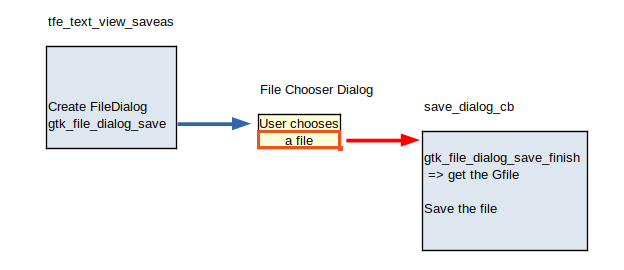
\includegraphics[width=10.7cm,height=5.16cm]{../image/saveas.png}
\caption{Saveas process}
\end{figure}

\subsection{Open related functions}\label{open-related-functions}

Open function shows a file chooser dialog to a user and prompts them to
choose a file. Then it reads the file and puts the text into
GtkTextBuffer.

\begin{lstlisting}[language=C]
void tfe_text_view_open (TfeTextView *tv, GtkWindow *win);
\end{lstlisting}

The parameter \passthrough{\lstinline!win!} is the transient window. A
file chooser dialog will be shown at the center of the window.

This function may be called just after \passthrough{\lstinline!tv!} has
been created. In that case, \passthrough{\lstinline!tv!} has not been
incorporated into the widget hierarchy. Therefore it is impossible to
get the top-level window from \passthrough{\lstinline!tv!}. That's why
the function needs \passthrough{\lstinline!win!} parameter.

This function is usually called when the buffer of
\passthrough{\lstinline!tv!} is empty. However, even if the buffer is
not empty, \passthrough{\lstinline!tfe\_text\_view\_open!} doesn't treat
it as an error. If you want to revert the buffer, calling this function
is appropriate.

Open and read process is divided into two phases. One is creating and
showing a file chooser dialog and the other is the callback function.
The former is \passthrough{\lstinline!tfe\_text\_view\_open!} and the
latter is \passthrough{\lstinline!open\_dialog\_cb!}.

\subsubsection{open\_dialog\_cb function}\label{open_dialog_cb-function}

\begin{lstlisting}[language=C, numbers=left]
static void
open_dialog_cb (GObject *source_object, GAsyncResult *res, gpointer data) {
  GtkFileDialog *dialog = GTK_FILE_DIALOG (source_object);
  TfeTextView *tv = TFE_TEXT_VIEW (data);
  GtkTextBuffer *tb = gtk_text_view_get_buffer (GTK_TEXT_VIEW (tv));
  GtkWidget *win = gtk_widget_get_ancestor (GTK_WIDGET (tv), GTK_TYPE_WINDOW);
  GFile *file;
  char *contents;
  gsize length;
  gboolean file_changed;
  GtkAlertDialog *alert_dialog;
  GError *err = NULL;

  if ((file = gtk_file_dialog_open_finish (dialog, res, &err)) != NULL
      && g_file_load_contents (file, NULL, &contents, &length, NULL, &err)) {
    gtk_text_buffer_set_text (tb, contents, length);
    g_free (contents);
    gtk_text_buffer_set_modified (tb, FALSE);
    // G_IS_FILE(tv->file) && tv->file == file => unref(tv->file), tv->file=file, emit response with SUCCESS
    // G_IS_FILE(tv->file) && tv->file != file => unref(tv->file), tv->file=file, emit response with SUCCESS, emit change-file
    // tv->file==NULL =>                                           tv->file=file, emit response with SUCCESS, emit change-file
    // The order is important. If you unref tv->file first, you can't compare tv->file and file anymore.
    // And the signals are emitted after new tv->file is set. Or the handler can't catch the new file.
    file_changed = (G_IS_FILE (tv->file) && g_file_equal (tv->file, file)) ? FALSE : TRUE;
    if (G_IS_FILE (tv->file))
      g_object_unref (tv->file);
    tv->file = file; // The ownership of 'file' moves to TfeTextView
    if (file_changed)
      g_signal_emit (tv, tfe_text_view_signals[CHANGE_FILE], 0);
    g_signal_emit (tv, tfe_text_view_signals[OPEN_RESPONSE], 0, TFE_OPEN_RESPONSE_SUCCESS);
  } else {
    if (err->code == GTK_DIALOG_ERROR_DISMISSED) // The user canceled the file chooser dialog
      g_signal_emit (tv, tfe_text_view_signals[OPEN_RESPONSE], 0, TFE_OPEN_RESPONSE_CANCEL);
    else {
      alert_dialog = gtk_alert_dialog_new ("%s", err->message);
      gtk_alert_dialog_show (alert_dialog, GTK_WINDOW (win));
      g_object_unref (alert_dialog);
      g_signal_emit (tv, tfe_text_view_signals[OPEN_RESPONSE], 0, TFE_OPEN_RESPONSE_ERROR);
    }
    g_clear_error (&err);
  }
}
\end{lstlisting}

This function is similar to \passthrough{\lstinline!save\_dialog\_cb!}.
Both are callback functions on a GtkFileDialog object.

\begin{itemize}
\tightlist
\item
  2: It has three parameters like
  \passthrough{\lstinline!save\_dialog\_cb!}. They are:

  \begin{itemize}
  \tightlist
  \item
    GObject *source\_object: The GObject instance that the operation was
    started with. It is actually the GtkFileDialog instance that is
    shown to the user. It will be casted to GtkFileDialog later.
  \item
    GAsyncResult *res: The result of the asynchronous operation. It will
    be given to the \passthrough{\lstinline!gtk\_dialog\_open\_finish!}
    function.
  \item
    gpointer data: A user data set in the
    \passthrough{\lstinline!gtk\_dialog\_open!} function. It is actually
    a TfeTextView instance and it will be casted to TfeTextView later.
  \end{itemize}
\item
  14: The function
  \passthrough{\lstinline!gtk\_file\_dialog\_open\_finish!} returns a
  GFile object if the operation has succeeded. Otherwise it returns
  NULL.
\item
  16-30: If the user selects a file and the file has successfully been
  read, the codes from 16 to 30 will be executed.
\item
  16-18: Sets the buffer of \passthrough{\lstinline!tv!} with the text
  read from the file. And frees \passthrough{\lstinline!contents!}. Then
  sets the modified status to false.
\item
  19-30: The codes are a bit complicated. See the comments. If the file
  (\passthrough{\lstinline!tv->file!}) is changed, ``change-file''
  signal is emitted. The signal ``open-response'' is emitted with the
  parameter \passthrough{\lstinline!TFE\_OPEN\_RESPONSE\_SUCCESS!}.
\item
  31-41: If the operation failed, the codes from 31 to 41 will be
  executed.
\item
  32-33: If the error code is
  \passthrough{\lstinline!GTK\_DIALOG\_ERROR\_DISMISSED!}, it means that
  the user has clicked on the ``Cancel'' button or close button on the
  header bar. Then, ``open-response'' signal is emitted with the
  parameter \passthrough{\lstinline!TFE\_OPEN\_RESPONSE\_CANCEL!}. The
  Dialog error is described
  \href{https://docs.gtk.org/gtk4/error.DialogError.html}{here} in the
  GTK API reference.
\item
  35-38: If another error occurs, it shows an alert dialog to report the
  error and emits ``open-response'' signal with the parameter
  \passthrough{\lstinline!TFE\_OPEN\_RESPONSE\_ERROR!}.
\item
  40: Clears the error structure.
\end{itemize}

\subsubsection{tfe\_text\_view\_open
function}\label{tfe_text_view_open-function}

\begin{lstlisting}[language=C, numbers=left]
void
tfe_text_view_open (TfeTextView *tv, GtkWindow *win) {
  g_return_if_fail (TFE_IS_TEXT_VIEW (tv));
  // 'win' is used for a transient window of the GtkFileDialog.
  // It can be NULL.
  g_return_if_fail (GTK_IS_WINDOW (win) || win == NULL);

  GtkFileDialog *dialog;

  dialog = gtk_file_dialog_new ();
  gtk_file_dialog_open (dialog, win, NULL, open_dialog_cb, tv);
  g_object_unref (dialog);
}
\end{lstlisting}

\begin{itemize}
\tightlist
\item
  3-6: Check the type of the arguments \passthrough{\lstinline!tv!} and
  \passthrough{\lstinline!win!}. Public functions always need to check
  the arguments.
\item
  10: Creates a GtkFileDialog instance.
\item
  11: Calls \passthrough{\lstinline!gtk\_file\_dialog\_open!}. The
  arguments are:

  \begin{itemize}
  \tightlist
  \item
    \passthrough{\lstinline!dialog!}: the GtkFileDialog instance
  \item
    \passthrough{\lstinline!win!}: the transient window for the file
    chooser dialog
  \item
    \passthrough{\lstinline!NULL!}: NULL means no cancellable object
  \item
    \passthrough{\lstinline!open\_dialog\_cb!}: callback function
  \item
    \passthrough{\lstinline!tv!}: user data which is used in the
    callback function
  \end{itemize}
\item
  12: Releases the dialog instance because it is useless anymore.
\end{itemize}

The whole process between the caller and TfeTextView is shown in the
following diagram. It is really complicated. Because
\passthrough{\lstinline!gtk\_file\_dialog\_open!} can't return the
status of the operation.

\begin{figure}
\centering
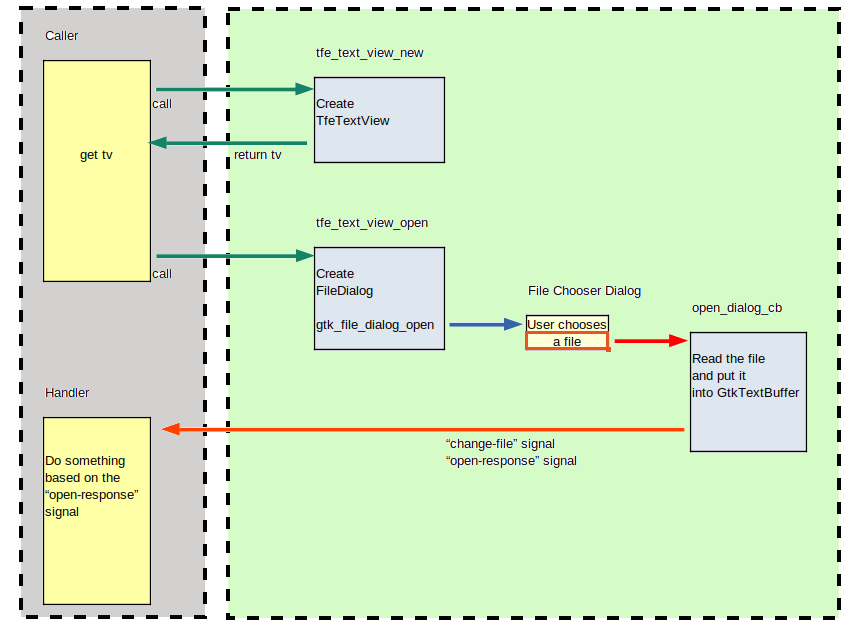
\includegraphics[width=12.405cm,height=9.225cm]{../image/open.png}
\caption{Caller and TfeTextView}
\end{figure}

\begin{enumerate}
\def\labelenumi{\arabic{enumi}.}
\tightlist
\item
  A caller gets a pointer \passthrough{\lstinline!tv!} to a TfeTextView
  instance by calling \passthrough{\lstinline!tfe\_text\_view\_new!}.
\item
  The caller connects the handler (left bottom in the diagram) and the
  signal ``open-response''.
\item
  It calls \passthrough{\lstinline!tfe\_text\_view\_open!} to prompt the
  user to select a file from the file chooser dialog.
\item
  When the dialog is closed, the callback
  \passthrough{\lstinline!open\_dialog\_cb!} is called.
\item
  The callback function reads the file and inserts the text into
  GtkTextBuffer and emits a signal to inform the status as a response
  code.
\item
  The handler of the ``open-response'' signal is invoked and the
  operation status is given to it as an argument (signal parameter).
\end{enumerate}

\subsection{Getting GFile in
TfeTextView}\label{getting-gfile-in-tfetextview}

You can get the GFile in a TfeTextView instance with
\passthrough{\lstinline!tfe\_text\_view\_get\_file!}. It is very simple.

\begin{lstlisting}[language=C, numbers=left]
GFile *
tfe_text_view_get_file (TfeTextView *tv) {
  g_return_val_if_fail (TFE_IS_TEXT_VIEW (tv), NULL);

  if (G_IS_FILE (tv->file))
    return g_file_dup (tv->file);
  else
    return NULL;
}
\end{lstlisting}

The important thing is to duplicate \passthrough{\lstinline!tv->file!}.
Otherwise, if the caller frees the GFile object,
\passthrough{\lstinline!tv->file!} is no more guaranteed to point the
GFile. Another reason to use \passthrough{\lstinline!g\_file\_dup!} is
that GFile isn't thread-safe. If you use GFile in the different thread,
the duplication is necessary. See
\href{https://docs.gtk.org/gio/method.File.dup.html}{Gio API Reference
-- g\_file\_dup}.

\subsection{The API document and source file of
tfetextview.c}\label{the-api-document-and-source-file-of-tfetextview.c}

Refer API document of TfeTextView in the appendix. The markdown file is
under the directory \passthrough{\lstinline!src/tfetextview!}.

You can find all the TfeTextView source codes under src/tfetextview
directories.

  \section{Functions in GtkNotebook}\label{functions-in-gtknotebook}

GtkNotebook is a very important object in the text file editor
\passthrough{\lstinline!tfe!}. It connects the application and
TfeTextView objects. A set of public functions are declared in
\passthrough{\lstinline!tfenotebook.h!}. The word ``tfenotebook'' is
used only in filenames. There's no ``TfeNotebook'' object.

The source files are in the directory
\passthrough{\lstinline!src/tfe5!}. You can get them by downloading the
\href{https://github.com/ToshioCP/Gtk4-tutorial}{repository}.

\begin{lstlisting}[language=C, numbers=left]
void
notebook_page_save(GtkNotebook *nb);

void
notebook_page_close (GtkNotebook *nb);

void
notebook_page_open (GtkNotebook *nb);

void
notebook_page_new_with_file (GtkNotebook *nb, GFile *file);

void
notebook_page_new (GtkNotebook *nb);
\end{lstlisting}

This header file describes the public functions in
\passthrough{\lstinline!tfenotebook.c!}.

\begin{itemize}
\tightlist
\item
  1-2: \passthrough{\lstinline!notebook\_page\_save!} saves the current
  page to the file of which the name specified in the tab. If the name
  is \passthrough{\lstinline!untitled!} or
  \passthrough{\lstinline!untitled!} followed by digits, a file chooser
  dialog appears and a user can choose or specify a filename.
\item
  4-5: \passthrough{\lstinline!notebook\_page\_close!} closes the
  current page.
\item
  7-8: \passthrough{\lstinline!notebook\_page\_open!} shows a file
  chooser dialog and a user can choose a file. The contents of the file
  is inserted to a new page.
\item
  10-11: \passthrough{\lstinline!notebook\_page\_new\_with\_file!}
  creates a new page and a file given as an argument is read and
  inserted into the page.
\item
  13-14: \passthrough{\lstinline!notebook\_page\_new!} creates a new
  empty page.
\end{itemize}

You probably find that the functions except
\passthrough{\lstinline!notebook\_page\_close!} are higher level
functions of

\begin{itemize}
\tightlist
\item
  \passthrough{\lstinline!tfe\_text\_view\_save!}
\item
  \passthrough{\lstinline!tef\_text\_view\_open!}
\item
  \passthrough{\lstinline!tfe\_text\_view\_new\_with\_file!}
\item
  \passthrough{\lstinline!tfe\_text\_view\_new!}
\end{itemize}

respectively.

There are two layers. One of them is
\passthrough{\lstinline!tfe\_text\_view ...!}, which is the lower level
layer. The other is \passthrough{\lstinline!notebook ...!}, which is the
higher level layer.

Now let's look at the program of each function.

\subsection{notebook\_page\_new}\label{notebook_page_new}

\begin{lstlisting}[language=C, numbers=left]
static char*
get_untitled () {
  static int c = -1;
  if (++c == 0) 
    return g_strdup_printf("Untitled");
  else
    return g_strdup_printf ("Untitled%u", c);
}

static void
notebook_page_build (GtkNotebook *nb, GtkWidget *tv, const char *filename) {
  GtkWidget *scr = gtk_scrolled_window_new ();
  GtkNotebookPage *nbp;
  GtkWidget *lab;
  int i;

  gtk_scrolled_window_set_child (GTK_SCROLLED_WINDOW (scr), tv);
  lab = gtk_label_new (filename);
  i = gtk_notebook_append_page (nb, scr, lab);
  nbp = gtk_notebook_get_page (nb, scr);
  g_object_set (nbp, "tab-expand", TRUE, NULL);
  gtk_notebook_set_current_page (nb, i);
  g_signal_connect (GTK_TEXT_VIEW (tv), "change-file", G_CALLBACK (file_changed_cb), nb);
}

void
notebook_page_new (GtkNotebook *nb) {
  g_return_if_fail(GTK_IS_NOTEBOOK (nb));

  GtkWidget *tv;
  char *filename;

  tv = tfe_text_view_new ();
  filename = get_untitled ();
  notebook_page_build (nb, tv, filename);
  g_free (filename);
}
\end{lstlisting}

\begin{itemize}
\tightlist
\item
  26-37: The function \passthrough{\lstinline!notebook\_page\_new!}.
\item
  28: The function \passthrough{\lstinline!g\_return\_if\_fail!} checks
  the argument. It's necessary because the function is public.
\item
  33: Creates TfeTextView object.
\item
  34: Creates filename, which is ``Untitled'', ``Untitled1'', \ldots{} .
\item
  1-8: The function \passthrough{\lstinline!get\_untitled!}.
\item
  3: Static variable \passthrough{\lstinline!c!} is initialized at the
  first call of this function. After that \passthrough{\lstinline!c!}
  keeps its value unless it is changed explicitly.
\item
  4-7: Increases \passthrough{\lstinline!c!} by one and if it is zero,
  it returns ``Untitled''. If it is a positive integer, it returns
  ``Untitled\textless the integer\textgreater{}'', for example,
  ``Untitled1'', ``Untitled2'', and so on. The function
  \passthrough{\lstinline!g\_strdup\_printf!} creates a string and it
  should be freed by \passthrough{\lstinline!g\_free!} when it becomes
  useless. The caller of \passthrough{\lstinline!get\_untitled!} is in
  charge of freeing the string.
\item
  36: Calls \passthrough{\lstinline!notebook\_page\_build!} to build a
  new page.
\item
  37: Frees \passthrough{\lstinline!filename!}.
\item
  10- 24: The function \passthrough{\lstinline!notebook\_page\_build!}.
  A parameter with \passthrough{\lstinline!const!} qualifier doesn't
  change in the function. It means that the argument
  \passthrough{\lstinline!filename!} is owned by the caller. The caller
  needs to free it when it becomes useless.
\item
  12: Creates GtkScrolledWindow.
\item
  17: Inserts \passthrough{\lstinline!tv!} to GtkScrolledWindow as a
  child.
\item
  18-19: Creates GtkLabel, then appends \passthrough{\lstinline!scr!}
  and \passthrough{\lstinline!lab!} to the GtkNotebook instance
  \passthrough{\lstinline!nb!}.
\item
  20-21: Sets ``tab-expand'' property to TRUE. The function
  \passthrough{\lstinline!g\_object\_set!} sets properties on an object.
  The object can be any object derived from GObject. In many cases, an
  object has its own function to set its properties, but sometimes
  doesn't. In that case, use \passthrough{\lstinline!g\_object\_set!} to
  set the property.
\item
  22: Sets the current page to the newly created page.
\item
  23: Connects ``change-file'' signal and the handler
  \passthrough{\lstinline!file\_changed\_cb!}.
\end{itemize}

\subsection{notebook\_page\_new\_with\_file}\label{notebook_page_new_with_file}

\begin{lstlisting}[language=C, numbers=left]
void
notebook_page_new_with_file (GtkNotebook *nb, GFile *file) {
  g_return_if_fail(GTK_IS_NOTEBOOK (nb));
  g_return_if_fail(G_IS_FILE (file));

  GtkWidget *tv;
  char *filename;

  if ((tv = tfe_text_view_new_with_file (file)) == NULL)
    return; /* read error */
  filename = g_file_get_basename (file);
  notebook_page_build (nb, tv, filename);
  g_free (filename);
}
\end{lstlisting}

\begin{itemize}
\tightlist
\item
  9-10: Calls
  \passthrough{\lstinline!tfe\_text\_view\_new\_with\_file!}. If the
  function returns NULL, an error has happened. Then, it does nothing
  and returns.
\item
  11-13: Gets the filename, builds a new page and frees
  \passthrough{\lstinline!filename!}.
\end{itemize}

\subsection{notebook\_page\_open}\label{notebook_page_open}

\begin{lstlisting}[language=C, numbers=left]
static void
open_response_cb (TfeTextView *tv, int response, GtkNotebook *nb) {
  GFile *file;
  char *filename;

  if (response != TFE_OPEN_RESPONSE_SUCCESS) {
    g_object_ref_sink (tv);
    g_object_unref (tv);
  }else {
    file = tfe_text_view_get_file (tv);
    filename = g_file_get_basename (file);
    g_object_unref (file);
    notebook_page_build (nb, GTK_WIDGET (tv), filename);
    g_free (filename);
  }
}

void
notebook_page_open (GtkNotebook *nb) {
  g_return_if_fail(GTK_IS_NOTEBOOK (nb));

  GtkWidget *tv;

  tv = tfe_text_view_new ();
  g_signal_connect (TFE_TEXT_VIEW (tv), "open-response", G_CALLBACK (open_response_cb), nb);
  tfe_text_view_open (TFE_TEXT_VIEW (tv), GTK_WINDOW (gtk_widget_get_ancestor (GTK_WIDGET (nb), GTK_TYPE_WINDOW)));
}
\end{lstlisting}

\begin{itemize}
\tightlist
\item
  18-27: The function \passthrough{\lstinline!notebook\_page\_open!}.
\item
  24: Creates TfeTextView object.
\item
  25: Connects the signal ``open-response'' and the handler
  \passthrough{\lstinline!open\_response\_cb!}.
\item
  26: Calls \passthrough{\lstinline!tfe\_text\_view\_open!}. The
  ``open-response'' signal will be emitted later in this function to
  inform the result.
\item
  1-16: The handler \passthrough{\lstinline!open\_response\_cb!}.
\item
  6-8: If the response code is not
  \passthrough{\lstinline!TFE\_OPEN\_RESPONSE\_SUCCESS!}, the instance
  \passthrough{\lstinline!tv!} will be destroyed. It has floating
  reference, which will be explained later. A floating reference needs
  to be converted into an ordinary reference before releasing it. The
  function \passthrough{\lstinline!g\_object\_ref\_sink!} does that.
  After that, the function \passthrough{\lstinline!g\_object\_unref!}
  releases \passthrough{\lstinline!tv!} and decreases the reference
  count by one. Finally the reference count becomes zero and
  \passthrough{\lstinline!tv!} is destroyed.
\item
  9-15: Otherwise, it builds a new page with
  \passthrough{\lstinline!tv!}.
\end{itemize}

\subsection{Floating reference}\label{floating-reference}

All the widgets are derived from GInitiallyUnowned. GObject and
GInitiallyUnowned are almost the same. The difference is like this. When
an instance of GInitiallyUnowned is created, the instance has a
``floating reference''. On the other hand, when an instance of GObject
(not GInitiallyUnowned) is created, it has ``normal reference''. Their
descendants inherits them, so every widget has a floating reference just
after the creation. Non-widget class, for example, GtkTextBuffer is a
direct sub class of GObject and it has normal reference.

The function \passthrough{\lstinline!g\_object\_ref\_sink!} converts the
floating reference into a normal reference. If the instance doesn't have
a floating reference, \passthrough{\lstinline!g\_object\_ref\_sink!}
simply increases the reference count by one. It is used when an widget
is added to another widget as a child.

\begin{lstlisting}
GtkTextView *tv = gtk_text_view_new (); // Floating reference
GtkScrolledWindow *scr = gtk_scrolled_window_new ();
gtk_scrolled_window_set_child (scr, tv); // Scrolled window sink the tv's floating reference and tv's reference count becomes one.
\end{lstlisting}

When \passthrough{\lstinline!tv!} is added to
\passthrough{\lstinline!scr!} as a child,
\passthrough{\lstinline!g\_object\_ref\_sink!} is used.

\begin{lstlisting}
g_object_ref_sink (tv);
\end{lstlisting}

So, the floating reference is converted into an ordinary reference. That
is to say, floating reference is removed, and the normal reference count
is one. Thanks to this, the caller doesn't need to decrease tv's
reference count. If an Object\_A is not a descendant of
GInitiallyUnowned, the program is like this:

\begin{lstlisting}
Object_A *obj_a = object_a_new (); // reference count is one
GtkScrolledWindow *scr = gtk_scrolled_window_new ();
gtk_scrolled_window_set_child (scr, obj_a); // obj_a's reference count is two
// obj_a is referred by the caller (this program) and scrolled window
g_object_unref (obj_a); // obj_a's reference count is one because the caller no longer refers obj_a.
\end{lstlisting}

This example tells us that the caller needs to unref
\passthrough{\lstinline!obj\_a!}.

If you use \passthrough{\lstinline!g\_object\_unref!} to an instance
that has a floating reference, you need to convert the floating
reference to a normal reference in advance. See
\href{https://docs.gtk.org/gobject/floating-refs.html}{GObject API
reference} for further information.

\subsection{notebook\_page\_close}\label{notebook_page_close}

\begin{lstlisting}[language=C, numbers=left]
void
notebook_page_close (GtkNotebook *nb) {
  g_return_if_fail(GTK_IS_NOTEBOOK (nb));

  GtkWidget *win;
  int i;

  if (gtk_notebook_get_n_pages (nb) == 1) {
    win = gtk_widget_get_ancestor (GTK_WIDGET (nb), GTK_TYPE_WINDOW);
    gtk_window_destroy(GTK_WINDOW (win));
  } else {
    i = gtk_notebook_get_current_page (nb);
    gtk_notebook_remove_page (GTK_NOTEBOOK (nb), i);
  }
}
\end{lstlisting}

This function closes the current page. If the page is the only page the
notebook has, then the function destroys the top-level window and quits
the application.

\begin{itemize}
\tightlist
\item
  8-10: If the page is the only page the notebook has, it calls
  \passthrough{\lstinline!gtk\_window\_destroy!} to destroy the
  top-level window.
\item
  11-13: Otherwise, removes the current page. The child widget
  (TfeTextView) is also destroyed.
\end{itemize}

\subsection{notebook\_page\_save}\label{notebook_page_save}

\begin{lstlisting}[language=C, numbers=left]
static TfeTextView *
get_current_textview (GtkNotebook *nb) {
  int i;
  GtkWidget *scr;
  GtkWidget *tv;

  i = gtk_notebook_get_current_page (nb);
  scr = gtk_notebook_get_nth_page (nb, i);
  tv = gtk_scrolled_window_get_child (GTK_SCROLLED_WINDOW (scr));
  return TFE_TEXT_VIEW (tv);
}

void
notebook_page_save (GtkNotebook *nb) {
  g_return_if_fail(GTK_IS_NOTEBOOK (nb));

  TfeTextView *tv;

  tv = get_current_textview (nb);
  tfe_text_view_save (tv);
}
\end{lstlisting}

\begin{itemize}
\tightlist
\item
  13-21: \passthrough{\lstinline!notebook\_page\_save!}.
\item
  19: Gets the TfeTextView instance belongs to the current page. The
  caller doesn't have the ownership of \passthrough{\lstinline!tv!} so
  you don't need to care about freeing it.
\item
  20: Calls \passthrough{\lstinline!tfe\_text\_view\_save!}.
\item
  1-11: \passthrough{\lstinline!get\_current\_textview!}. This function
  gets the TfeTextView object belongs to the current page.
\item
  7: Gets the page number of the current page.
\item
  8: Gets the child widget \passthrough{\lstinline!scr!}, which is a
  GtkScrolledWindow instance, of the current page. The object
  \passthrough{\lstinline!scr!} is owned by the notebook
  \passthrough{\lstinline!nb!}. So, the caller doesn't need to free it.
\item
  9-10: Gets the child widget of \passthrough{\lstinline!scr!}, which is
  a TfeTextView instance, and returns it. The returned instance is owned
  by \passthrough{\lstinline!scr!} and the caller of
  \passthrough{\lstinline!get\_cuurent\_textview!} doesn't need to care
  about freeing it.
\end{itemize}

\subsection{file\_changed\_cb handler}\label{file_changed_cb-handler}

The function \passthrough{\lstinline!file\_changed\_cb!} is a handler
connected to ``change-file'' signal. If a file in a TfeTextView instance
is changed, the instance emits this signal. This handler changes the
label of the GtkNotebookPage.

\begin{lstlisting}[language=C, numbers=left]
static void
file_changed_cb (TfeTextView *tv, GtkNotebook *nb) {
  GtkWidget *scr;
  GtkWidget *label;
  GFile *file;
  char *filename;

  file = tfe_text_view_get_file (tv);
  scr = gtk_widget_get_parent (GTK_WIDGET (tv));
  if (G_IS_FILE (file)) {
    filename = g_file_get_basename (file);
    g_object_unref (file);
  } else
    filename = get_untitled ();
  label = gtk_label_new (filename);
  g_free (filename);
  gtk_notebook_set_tab_label (nb, scr, label);
}
\end{lstlisting}

\begin{itemize}
\tightlist
\item
  8: Gets the GFile instance from \passthrough{\lstinline!tv!}.
\item
  9: Gets the GkScrolledWindow instance which is the parent widget of
  \passthrough{\lstinline!tv!}.
\item
  10-12: If \passthrough{\lstinline!file!} points a GFile instance, the
  filename of the GFile is assigned to
  \passthrough{\lstinline!filename!}. Then, unref the GFile object
  \passthrough{\lstinline!file!}.
\item
  13-14: Otherwise (file is NULL), a string
  \passthrough{\lstinline!Untitled(number)!} is assigned to
  \passthrough{\lstinline!filename!}.
\item
  15-17: Creates a GtkLabel instance \passthrough{\lstinline!label!}
  with the filename and set the label of the GtkNotebookPage with
  \passthrough{\lstinline!label!}.
\end{itemize}

  \section{Tfe main program}\label{tfe-main-program}

The file \passthrough{\lstinline!tfeapplication.c!} is a main program of
Tfe. It includes all the code other than
\passthrough{\lstinline!tfetextview.c!} and
\passthrough{\lstinline!tfenotebook.c!}. It does:

\begin{itemize}
\tightlist
\item
  Application support, mainly handling command line arguments.
\item
  Builds widgets using ui file.
\item
  Connects button signals and their handlers.
\item
  Manages CSS.
\end{itemize}

\subsection{The function main}\label{the-function-main}

The function \passthrough{\lstinline!main!} is the first invoked
function in C language. It connects the command line given by the user
and Gtk application.

\begin{lstlisting}[language=C, numbers=left]
#define APPLICATION_ID "com.github.ToshioCP.tfe"

int
main (int argc, char **argv) {
  GtkApplication *app;
  int stat;

  app = gtk_application_new (APPLICATION_ID, G_APPLICATION_HANDLES_OPEN);

  g_signal_connect (app, "startup", G_CALLBACK (app_startup), NULL);
  g_signal_connect (app, "activate", G_CALLBACK (app_activate), NULL);
  g_signal_connect (app, "open", G_CALLBACK (app_open), NULL);

  stat =g_application_run (G_APPLICATION (app), argc, argv);
  g_object_unref (app);
  return stat;
}
\end{lstlisting}

\begin{itemize}
\tightlist
\item
  1: Defines the application id. Thanks to the
  \passthrough{\lstinline!\#define!} directive, it is easy to find the
  application id.
\item
  8: Creates GtkApplication object.
\item
  10-12: Connects ``startup'', ``activate'' and ``open'' signals to
  their handlers.
\item
  14: Runs the application.
\item
  15-16: Releases the reference to the application and returns the
  status.
\end{itemize}

\subsection{Startup signal handler}\label{startup-signal-handler}

Startup signal is emitted just after the GtkApplication instance is
initialized. The handler initializes the whole application which
includes not only GtkApplication instance but also widgets and some
other objects.

\begin{itemize}
\tightlist
\item
  Builds the widgets using ui file.
\item
  Connects button signals and their handlers.
\item
  Sets CSS.
\end{itemize}

The handler is as follows.

\begin{lstlisting}[language=C, numbers=left]
static void
app_startup (GApplication *application) {
  GtkApplication *app = GTK_APPLICATION (application);
  GtkBuilder *build;
  GtkApplicationWindow *win;
  GtkNotebook *nb;
  GtkButton *btno;
  GtkButton *btnn;
  GtkButton *btns;
  GtkButton *btnc;

  build = gtk_builder_new_from_resource ("/com/github/ToshioCP/tfe/tfe.ui");
  win = GTK_APPLICATION_WINDOW (gtk_builder_get_object (build, "win"));
  nb = GTK_NOTEBOOK (gtk_builder_get_object (build, "nb"));
  gtk_window_set_application (GTK_WINDOW (win), app);
  btno = GTK_BUTTON (gtk_builder_get_object (build, "btno"));
  btnn = GTK_BUTTON (gtk_builder_get_object (build, "btnn"));
  btns = GTK_BUTTON (gtk_builder_get_object (build, "btns"));
  btnc = GTK_BUTTON (gtk_builder_get_object (build, "btnc"));
  g_signal_connect_swapped (btno, "clicked", G_CALLBACK (open_cb), nb);
  g_signal_connect_swapped (btnn, "clicked", G_CALLBACK (new_cb), nb);
  g_signal_connect_swapped (btns, "clicked", G_CALLBACK (save_cb), nb);
  g_signal_connect_swapped (btnc, "clicked", G_CALLBACK (close_cb), nb);
  g_object_unref(build);

GdkDisplay *display;

  display = gdk_display_get_default ();
  GtkCssProvider *provider = gtk_css_provider_new ();
  gtk_css_provider_load_from_data (provider, "textview {padding: 10px; font-family: monospace; font-size: 12pt;}", -1);
  gtk_style_context_add_provider_for_display (display, GTK_STYLE_PROVIDER (provider), GTK_STYLE_PROVIDER_PRIORITY_APPLICATION);

  g_signal_connect (win, "destroy", G_CALLBACK (before_destroy), provider);
  g_object_unref (provider);
}
\end{lstlisting}

\begin{itemize}
\tightlist
\item
  12-15: Builds widgets using ui resource. Connects the top-level window
  and the application with
  \passthrough{\lstinline!gtk\_window\_set\_application!}.
\item
  16-23: Gets buttons and connects their signals and handlers. The macro
  \passthrough{\lstinline!g\_signal\_connect\_swapped!} connects a
  signal and handler like \passthrough{\lstinline!g\_signal\_connect!}.
  The difference is that
  \passthrough{\lstinline!g\_signal\_connect\_swapped!} swaps the user
  data for the object. For example, the macro on line 20 swaps
  \passthrough{\lstinline!nb!} for \passthrough{\lstinline!btno!}. So,
  the handler expects that the first argument is
  \passthrough{\lstinline!nb!} instead of
  \passthrough{\lstinline!btno!}.
\item
  24: Releases the reference to GtkBuilder.
\item
  26-31: Sets CSS. CSS in Gtk is similar to CSS in HTML. You can set
  margin, border, padding, color, font and so on with CSS. In this
  program, CSS is on line 30. It sets padding, font-family and font size
  of GtkTextView. CSS will be explained in the next subsection.
\item
  26-28: GdkDisplay is used to set CSS. The default GdkDisplay object
  can be obtain with the function
  \passthrough{\lstinline!gfk\_display\_get\_default!}. This function
  needs to be called after the window creation.
\item
  33: Connects ``destroy'' signal on the main window and before\_destroy
  handler. This handler is explained in the next subsection.
\item
  34: The provider is useless for the startup handler, so it is
  released. Note: It doesn't mean the destruction of the provider. It is
  referred by the display so the reference count is not zero.
\end{itemize}

\subsection{CSS in Gtk}\label{css-in-gtk}

CSS is an abbreviation of Cascading Style Sheet. It is originally used
with HTML to describe the presentation semantics of a document. You
might have found that widgets in Gtk is similar to elements in HTML. It
tells that CSS can be applied to Gtk windowing system, too.

\subsubsection{CSS nodes, selectors}\label{css-nodes-selectors}

The syntax of CSS is as follows.

\begin{lstlisting}
selector { color: yellow; padding-top: 10px; ...}
\end{lstlisting}

Every widget has CSS node. For example, GtkTextView has
\passthrough{\lstinline!textview!} node. If you want to set style to
GtkTextView, substitute ``textview'' for
\passthrough{\lstinline!selector!} above.

\begin{lstlisting}
textview {color: yellow; ...}
\end{lstlisting}

Class, ID and some other things can be applied to the selector like Web
CSS. Refer to \href{https://docs.gtk.org/gtk4/css-overview.html}{GTK 4
API Reference -- CSS in Gtk} for further information.

The codes of the startup handler has a CSS string on line 30.

\begin{lstlisting}
textview {padding: 10px; font-family: monospace; font-size: 12pt;}
\end{lstlisting}

\begin{itemize}
\tightlist
\item
  Padding is a space between the border and contents. This space makes
  the textview easier to read.
\item
  font-family is a name of font. The font name ``monospace'' is one of
  the generic family font keywords.
\item
  Font-size is set to 12pt.
\end{itemize}

\subsubsection{GtkStyleContext, GtkCssProvider and
GdkDisplay}\label{gtkstylecontext-gtkcssprovider-and-gdkdisplay}

GtkStyleContext is deprecated since version 4.10. But two functions
\passthrough{\lstinline!gtk\_style\_context\_add\_provider\_for\_display!}
and
\passthrough{\lstinline!gtk\_style\_context\_remove\_provider\_for\_display!}
are not deprecated. They add or remove a css provider object to the
GdkDisplay object.

GtkCssProvider is an object which parses CSS for style widgets.

To apply your CSS to widgets, you need to add GtkStyleProvider (the
interface of GtkCssProvider) to the GdkDisplay object. You can get the
default display object with the function
\passthrough{\lstinline!gdk\_display\_get\_default!}. The returned
object is owned by the function and you don't have its ownership. So,
you don't need to care about releasing it.

Look at the source file of \passthrough{\lstinline!startup!} handler
again.

\begin{itemize}
\tightlist
\item
  28: The display is obtained by
  \passthrough{\lstinline!gdk\_display\_get\_default!}.
\item
  29: Creates a GtkCssProvider instance.
\item
  30: Puts the CSS into the provider. The function
  \passthrough{\lstinline!gtk\_css\_provider\_load\_from\_data!} will be
  deprecated since 4.12 (Not 4.10). The new function
  \passthrough{\lstinline!gtk\_css\_provider\_load\_from\_string!} will
  be used in the future version of Tfe.
\item
  31: Adds the provider to the display. The last argument of
  \passthrough{\lstinline!gtk\_style\_context\_add\_provider\_for\_display!}
  is the priority of the style provider.
  \passthrough{\lstinline!GTK\_STYLE\_PROVIDER\_PRIORITY\_APPLICATION!}
  is a priority for application-specific style information. Refer to
  \href{https://docs.gtk.org/gtk4/index.html\#constants}{GTK 4 Reference
  --- Constants} for more information. You can find other constants,
  which have ``STYLE\_PROVIDER\_PRIORITY\_XXXX'' pattern names.
\end{itemize}

\begin{lstlisting}[language=C, numbers=left]
static void
before_destroy (GtkWidget *win, GtkCssProvider *provider) {
  GdkDisplay *display = gdk_display_get_default ();
  gtk_style_context_remove_provider_for_display (display, GTK_STYLE_PROVIDER (provider));
}
\end{lstlisting}

When a widget is destroyed, or more precisely during its disposing
process, a ``destroy'' signal is emitted. The ``before\_destroy''
handler connects to the signal on the main window. (See the program list
of app\_startup.) So, it is called when the window is destroyed.

The handler removes the CSS provider from the GdkDisplay.

Note: CSS providers are removed automatically when the application
quits. So, even if the handler \passthrough{\lstinline!before\_destroy!}
is removed, the application works.

\subsection{Activate and open signal
handler}\label{activate-and-open-signal-handler}

The handlers of ``activate'' and ``open'' signals are
\passthrough{\lstinline!app\_activate!} and
\passthrough{\lstinline!app\_open!} respectively. They just create a new
GtkNotebookPage.

\begin{lstlisting}[language=C, numbers=left]
static void
app_activate (GApplication *application) {
  GtkApplication *app = GTK_APPLICATION (application);
  GtkWidget *win = GTK_WIDGET (gtk_application_get_active_window (app));
  GtkWidget *boxv = gtk_window_get_child (GTK_WINDOW (win));
  GtkNotebook *nb = GTK_NOTEBOOK (gtk_widget_get_last_child (boxv));

  notebook_page_new (nb);
  gtk_window_present (GTK_WINDOW (win));
}

static void
app_open (GApplication *application, GFile ** files, gint n_files, const gchar *hint) {
  GtkApplication *app = GTK_APPLICATION (application);
  GtkWidget *win = GTK_WIDGET (gtk_application_get_active_window (app));
  GtkWidget *boxv = gtk_window_get_child (GTK_WINDOW (win));
  GtkNotebook *nb = GTK_NOTEBOOK (gtk_widget_get_last_child (boxv));
  int i;

  for (i = 0; i < n_files; i++)
    notebook_page_new_with_file (nb, files[i]);
  if (gtk_notebook_get_n_pages (nb) == 0)
    notebook_page_new (nb);
  gtk_window_present (GTK_WINDOW (win));
}
\end{lstlisting}

\begin{itemize}
\tightlist
\item
  1-10: \passthrough{\lstinline!app\_activate!}.
\item
  8-10: Creates a new page and shows the window.
\item
  12-25: \passthrough{\lstinline!app\_open!}.
\item
  20-21: Creates notebook pages with files.
\item
  22-23: If no page has created, maybe because of read error, then it
  creates an empty page.
\item
  24: Shows the window.
\end{itemize}

These codes have become really simple thanks to tfenotebook.c and
tfetextview.c.

\subsection{A primary instance}\label{a-primary-instance}

Only one GApplication instance can be run at a time in a session. The
session is a bit difficult concept and also platform-dependent, but
roughly speaking, it corresponds to a graphical desktop login. When you
use your PC, you probably login first, then your desktop appears until
you log off. This is the session.

However, Linux is multi process OS and you can run two or more instances
of the same application. Isn't it a contradiction?

When first instance is launched, then it registers itself with its
application ID (for example,
\passthrough{\lstinline!com.github.ToshioCP.tfe!}). Just after the
registration, startup signal is emitted, then activate or open signal is
emitted and the instance's main loop runs. I wrote ``startup signal is
emitted just after the application instance is initialized'' in the
prior subsection. More precisely, it is emitted after the registration.

If another instance which has the same application ID is launched, it
also tries to register itself. Because this is the second instance, the
registration of the ID has already done, so it fails. Because of the
failure startup signal isn't emitted. After that, activate or open
signal is emitted in the primary instance, not on the second instance.
The primary instance receives the signal and its handler is invoked. On
the other hand, the second instance doesn't receive the signal and it
immediately quits.

Try running two instances in a row.

\begin{lstlisting}
$ ./_build/tfe &
[1] 84453
$ ./build/tfe tfeapplication.c
$
\end{lstlisting}

First, the primary instance opens a window. Then, after the second
instance is run, a new notebook page with the contents of
\passthrough{\lstinline!tfeapplication.c!} appears in the primary
instance's window. This is because the open signal is emitted in the
primary instance. The second instance immediately quits so shell prompt
soon appears.

\subsection{A series of handlers correspond to the button
signals}\label{a-series-of-handlers-correspond-to-the-button-signals}

\begin{lstlisting}[language=C, numbers=left]
static void
open_cb (GtkNotebook *nb) {
  notebook_page_open (nb);
}

static void
new_cb (GtkNotebook *nb) {
  notebook_page_new (nb);
}

static void
save_cb (GtkNotebook *nb) {
  notebook_page_save (nb);
}

static void
close_cb (GtkNotebook *nb) {
  notebook_page_close (GTK_NOTEBOOK (nb));
}
\end{lstlisting}

\passthrough{\lstinline!open\_cb!}, \passthrough{\lstinline!new\_cb!},
\passthrough{\lstinline!save\_cb!} and
\passthrough{\lstinline!close\_cb!} just call corresponding notebook
page functions.

\subsection{meson.build}\label{meson.build}

\begin{lstlisting}[numbers=left]
project('tfe', 'c')

gtkdep = dependency('gtk4')

gnome=import('gnome')
resources = gnome.compile_resources('resources','tfe.gresource.xml')

sourcefiles=files('tfeapplication.c', 'tfenotebook.c', '../tfetextview/tfetextview.c')

executable('tfe', sourcefiles, resources, dependencies: gtkdep)
\end{lstlisting}

In this file, just the source file names are modified from the prior
version.

\subsection{source files}\label{source-files}

You can download the files from the
\href{https://github.com/ToshioCP/Gtk4-tutorial}{repository}. There are
two options.

\begin{itemize}
\tightlist
\item
  Use git and clone.
\item
  Run your browser and open the
  \href{https://github.com/ToshioCP/Gtk4-tutorial}{top page}. Then click
  on ``Code'' button and click ``Download ZIP'' in the popup menu. After
  that, unzip the archive file.
\end{itemize}

If you use git, run the terminal and type the following.

\begin{lstlisting}
$ git clone https://github.com/ToshioCP/Gtk4-tutorial.git
\end{lstlisting}

The source files are under /src/tfe5 directory.

  \section{How to build tfe (text file
editor)}\label{how-to-build-tfe-text-file-editor}

\subsection{How to compile and execute the text editor
`tfe'.}\label{how-to-compile-and-execute-the-text-editor-tfe.}

First, source files are in the
\href{https://github.com/ToshioCP/Gtk4-tutorial}{Gtk4-tutorila
repository}. How to download them is written at the end of the previous
section.

The following is the instruction of compilation and execution.

\begin{itemize}
\tightlist
\item
  You need meson and ninja.
\item
  If you have installed gtk4 from the source, you need to set
  environment variables to suit your installation.
\item
  Change your current directory to \passthrough{\lstinline!src/tfe5!}
  directory.
\item
  Type \passthrough{\lstinline!meson setup \_build!} for configuration.
\item
  Type \passthrough{\lstinline!ninja -C \_build!} for compilation. Then
  the application \passthrough{\lstinline!tfe!} is built under the
  \passthrough{\lstinline!\_build!} directory.
\item
  Type \passthrough{\lstinline!\_build/tfe!} to execute it.
\end{itemize}

Then the window appears. There are four buttons,
\passthrough{\lstinline!New!}, \passthrough{\lstinline!Open!},
\passthrough{\lstinline!Save!} and \passthrough{\lstinline!Close!}.

\begin{itemize}
\tightlist
\item
  Click on \passthrough{\lstinline!Open!} button, then a file chooser
  dialog appears. Choose a file in the list and click on
  \passthrough{\lstinline!Open!} button. Then the file is read and a new
  Notebook Page appears.
\item
  Edit the file and click on \passthrough{\lstinline!Save!} button, then
  the text is saved to the original file.
\item
  Click \passthrough{\lstinline!Close!}, then the Notebook Page
  disappears.
\item
  Click \passthrough{\lstinline!Close!} again, then the
  \passthrough{\lstinline!Untitled!} Notebook Page disappears and at the
  same time the application quits.
\end{itemize}

This is a very simple editor. It is a good practice for you to add more
features.

\subsection{Total number of lines, words and
characters}\label{total-number-of-lines-words-and-characters}

\begin{lstlisting}
$ LANG=C wc tfe5/meson.build tfe5/tfeapplication.c tfe5/tfe.gresource.xml tfe5/tfenotebook.c tfe5/tfenotebook.h tfetextview/tfetextview.c tfetextview/tfetextview.h tfe5/tfe.ui
   10    17   294 tfe5/meson.build
  110   334  3601 tfe5/tfeapplication.c
    6     9   153 tfe5/tfe.gresource.xml
  144   390  3668 tfe5/tfenotebook.c
   15    21   241 tfe5/tfenotebook.h
  235   821  8473 tfetextview/tfetextview.c
   32    54   624 tfetextview/tfetextview.h
   61   100  2073 tfe5/tfe.ui
  613  1746 19127 total
\end{lstlisting}

  \section{Menus and actions}\label{menus-and-actions}

\subsection{Menus}\label{menus}

Users often use menus to tell a command to the application. It is like
this:

\begin{figure}
\centering
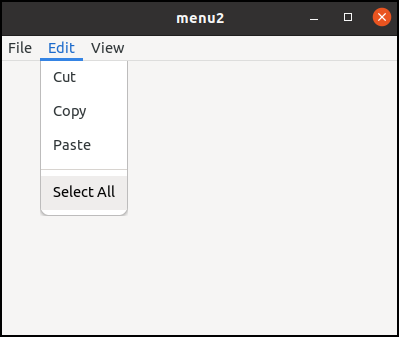
\includegraphics[width=5.985cm,height=5.055cm]{../image/menu.png}
\caption{Menu}
\end{figure}

There are two types of objects.

\begin{itemize}
\tightlist
\item
  ``File'', ``Edit'', ``View'', ``Cut'', ``Copy'', ``Paste'' and
  ``Select All''. They are called ``menu item'' or simply ``item''. When
  the user clicks one of these items, then something will happen.
\item
  Menubar, submenu referenced by ``Edit'' item and two sections. They
  are called ``menu''. Menu is an ordered list of items. They are
  similar to arrays.
\end{itemize}

\begin{figure}
\centering
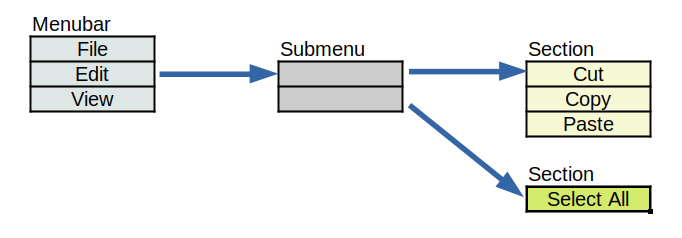
\includegraphics[width=10.23cm,height=3.57cm]{../image/menu_structure.png}
\caption{Menu structure}
\end{figure}

\begin{itemize}
\tightlist
\item
  Menubar is a menu which has three items, which are ``File'', ``Edit''
  and ``View''.
\item
  The menu item labeled ``Edit'' has a link to the submenu which has two
  items. These two items don't have labels. Each item refers to a
  section.
\item
  The first section is a menu which has three items -- ``Cut'', ``Copy''
  and ``Paste''.
\item
  The second section is a menu which has one item -- ``Select All''.
\end{itemize}

Menus can build a complicated structure thanks to the links of menu
items.

\subsection{GMenuModel, GMenu and
GMenuItem}\label{gmenumodel-gmenu-and-gmenuitem}

GMenuModel is an abstract object which represents a menu. GMenu is a
simple implementation of GMenuModel and a child object of GMenuModel.

\begin{lstlisting}
GObject -- GMenuModel -- GMenu
\end{lstlisting}

Because GMenuModel is an abstract object, it isn't instantiatable.
Therefore, it doesn't have any functions to create its instance. If you
want to create a menu, use \passthrough{\lstinline!g\_menu\_new!} to
create a GMenu instance. GMenu inherits all the functions of GMenuModel.

GMenuItem is an object directly derived from GObject. GMenuItem and
Gmenu (or GMenuModel) don't have a parent-child relationship.

\begin{lstlisting}
GObject -- GMenuModel -- GMenu
GObject -- GMenuItem
\end{lstlisting}

GMenuItem has attributes. One of the attributes is label. For example,
there is a menu item which has ``Edit'' label in the first diagram.
``Cut'', ``Copy'', ``Paste'' and ``Select All'' are also the labels of
the menu items. Other attributes will be explained later.

Some menu items have a link to another GMenu. There are two types of
links, submenu and section.

GMenuItem can be inserted, appended or prepended to GMenu. When it is
inserted, all of the attributes and link values are copied and stored in
the menu. The GMenuItem itself is not really inserted. Therefore, after
the insertion, GMenuItem is useless and it should be freed. The same
goes for appending or prepending.

The following code shows how to append GMenuItem to GMenu.

\begin{lstlisting}
GMenu *menu = g_menu_new ();
GMenuItem *menu_item_quit = g_menu_item_new ("Quit", "app.quit");
g_menu_append_item (menu, menu_item_quit);
g_object_unref (menu_item_quit);
\end{lstlisting}

\subsection{Menu and action}\label{menu-and-action}

One of the attributes of menu items is an action. This attribute points
an action object.

There are two action objects, GSimpleAction and GPropertyAction.
GSimpleAction is often used. And it is used with a menu item. Only
GSimpleAction is described in this section.

An action corresponds to a menu item will be activated when the menu
item is clicked. Then the action emits an activate signal.

\begin{enumerate}
\def\labelenumi{\arabic{enumi}.}
\tightlist
\item
  menu item is clicked.
\item
  The corresponding action is activated.
\item
  The action emits a signal.
\item
  The connected handler is invoked.
\end{enumerate}

The following code is an example.

\begin{lstlisting}[language=C]
static void
quit_activated(GSimpleAction *action, GVariant *parameter, gpointer app) { ... ... ...}

GSimpleAction *act_quit = g_simple_action_new ("quit", NULL);
g_action_map_add_action (G_ACTION_MAP (app), G_ACTION (act_quit));
g_signal_connect (act_quit, "activate", G_CALLBACK (quit_activated), app);
GMenuItem *menu_item_quit = g_menu_item_new ("Quit", "app.quit");
\end{lstlisting}

\begin{itemize}
\tightlist
\item
  The variable \passthrough{\lstinline!menu\_item\_quit!} points a menu
  item. It is actually a pointer, but we often say that
  \passthrough{\lstinline!menu\_item\_quit!} \emph{is} a menu item. It
  has a label ``Quit'' and is connected to an action ``app.quit''.
  ``app'' is a prefix and ``quit'' is the name of the action. The prefix
  ``app'' means that the action belongs to the GtkApplication instance.
\item
  \passthrough{\lstinline!act\_quit!} is an action. It has a name
  ``quit''. The function
  \passthrough{\lstinline!g\_simple\_action\_new!} creates a stateless
  action. So, \passthrough{\lstinline!act\_quit!} is stateless. The
  meaning of stateless will be explained later. The argument
  \passthrough{\lstinline!NULL!} means that the action doesn't have an
  parameter. Most of the actions are stateless and have no parameter.
\item
  The action \passthrough{\lstinline!act\_quit!} is added to the
  GtkApplication instance with
  \passthrough{\lstinline!g\_action\_map\_add\_action!}. So, the
  action's scope is application. The prefix of
  \passthrough{\lstinline!app.quit!} indicates the scope.
\item
  ``activate'' signal of the action is connected to the handler
  \passthrough{\lstinline!quit\_activated!}.
\end{itemize}

If the menu is clicked, the corresponding action ``quit'' will be
activated and emits an ``activate'' signal. Then, the handler
\passthrough{\lstinline!quit\_activated!} is called.

\subsection{Menu bar}\label{menu-bar}

A menu bar and menus are traditional. Menu buttons are often used
instead of a menu bar lately, but the old style is still used widely.

Applications have only one menu bar. If an application has two or more
windows which have menu bars, the menu bars are exactly the same.
Because every window refers to the same menubar instance in the
application.

An application's menu bar is usually unchanged once it is set. So, it is
appropriate to set it in the ``startup'' handler. Because the handler is
called only once in the primary application instance.

I think it is good for readers to clarify how applications behave.

\begin{itemize}
\tightlist
\item
  When an application runs for the first time, the instance is called
  primary.
\item
  The primary instance registers itself to the system. If it succeeds,
  it emits ``startup'' signal.
\item
  When the instance is activated, an ``activate'' or ``open'' signal is
  emitted.
\item
  If the application is run for the second time or later and there
  exists a primary instance, the instance is called a remote instance.
\item
  A remote instance doesn't emit ``startup'' signal.
\item
  If it tries to emit an ``activate'' or ``open'' signal, the signals
  are not emitted on the remote instance but primary instance.
\item
  The remote instance quits.
\end{itemize}

Therefore, an ``activate'' or ``open'' handler can be called twice or
more. On the other hand, a ``startup'' handler is called once. So, the
menubar should be set in the ``startup'' handler.

\begin{lstlisting}[language=C]
static void
app_startup (GApplication *app) {
... ... ...
  gtk_application_set_menubar (GTK_APPLICATION (app), G_MENU_MODEL (menubar));
... ... ...
}
\end{lstlisting}

\subsection{Simple example}\label{simple-example}

The following is a simple example of menus and actions. The source file
\passthrough{\lstinline!menu1.c!} is located at src/menu directory.

\begin{lstlisting}[language=C, numbers=left]
#include <gtk/gtk.h>

static void
quit_activated(GSimpleAction *action, GVariant *parameter, GApplication *application) {
  g_application_quit (application);
}

static void
app_activate (GApplication *application) {
  GtkApplication *app = GTK_APPLICATION (application);
  GtkWidget *win = gtk_application_window_new (app);
  gtk_window_set_title (GTK_WINDOW (win), "menu1");
  gtk_window_set_default_size (GTK_WINDOW (win), 400, 300);

  gtk_application_window_set_show_menubar (GTK_APPLICATION_WINDOW (win), TRUE);
  gtk_window_present (GTK_WINDOW (win));
}

static void
app_startup (GApplication *application) {
  GtkApplication *app = GTK_APPLICATION (application);

  GSimpleAction *act_quit = g_simple_action_new ("quit", NULL);
  g_action_map_add_action (G_ACTION_MAP (app), G_ACTION (act_quit));
  g_signal_connect (act_quit, "activate", G_CALLBACK (quit_activated), application);

  GMenu *menubar = g_menu_new ();
  GMenuItem *menu_item_menu = g_menu_item_new ("Menu", NULL);
  GMenu *menu = g_menu_new ();
  GMenuItem *menu_item_quit = g_menu_item_new ("Quit", "app.quit");
  g_menu_append_item (menu, menu_item_quit);
  g_object_unref (menu_item_quit);
  g_menu_item_set_submenu (menu_item_menu, G_MENU_MODEL (menu));
  g_object_unref (menu);
  g_menu_append_item (menubar, menu_item_menu);
  g_object_unref (menu_item_menu);

  gtk_application_set_menubar (GTK_APPLICATION (app), G_MENU_MODEL (menubar));
}

#define APPLICATION_ID "com.github.ToshioCP.menu1"

int
main (int argc, char **argv) {
  GtkApplication *app;
  int stat;

  app = gtk_application_new (APPLICATION_ID, G_APPLICATION_DEFAULT_FLAGS);
  g_signal_connect (app, "startup", G_CALLBACK (app_startup), NULL);
  g_signal_connect (app, "activate", G_CALLBACK (app_activate), NULL);

  stat =g_application_run (G_APPLICATION (app), argc, argv);
  g_object_unref (app);
  return stat;
}
\end{lstlisting}

\begin{itemize}
\tightlist
\item
  3-6: \passthrough{\lstinline!quit\_activated!} is a handler of the
  ``activate'' signal on the action \passthrough{\lstinline!act\_quit!}.
  Handlers of the ``activate'' signal have three parameters.

  \begin{enumerate}
  \def\labelenumi{\arabic{enumi}.}
  \tightlist
  \item
    The action instance on which the signal is emitted.
  \item
    Parameter. In this example it is \passthrough{\lstinline!NULL!}
    because the second argument of
    \passthrough{\lstinline!g\_simple\_action\_new!} (line 23) is
    \passthrough{\lstinline!NULL!}. You don' t need to care about it.
  \item
    User data. It is the fourth parameter in the
    \passthrough{\lstinline!g\_signal\_connect!} (line 25) that connects
    the action and the handler.
  \end{enumerate}
\item
  5: The function \passthrough{\lstinline!g\_application\_quit!}
  immediately quits the application.
\item
  8-17: \passthrough{\lstinline!app\_activate!} is an ``activate''
  signal handler on the application.
\item
  11-13: Creates a GtkApplicationWindow \passthrough{\lstinline!win!}.
  And sets the title and the default size.
\item
  15: Sets GtkApplicationWindow to show the menubar.
\item
  16: Shows the window.
\item
  19-38: \passthrough{\lstinline!app\_startup!} is a ``startup'' signal
  handler on the application.
\item
  23: Creates GSimpleAction \passthrough{\lstinline!act\_quit!}. It is
  stateless. The first argument of
  \passthrough{\lstinline!g\_simple\_action\_new!} is a name of the
  action and the second argument is a parameter. If you don't need the
  parameter, pass \passthrough{\lstinline!NULL!}. Therefore,
  \passthrough{\lstinline!act\_quit!} has a name ``quit'' and no
  parameter.
\item
  24: Adds the action to GtkApplication \passthrough{\lstinline!app!}.
  GtkApplication implements an interface GActionMap and GActionGroup.
  GtkApplication (GActionMap) can have a group of actions and the
  actions are added with the function
  \passthrough{\lstinline!g\_action\_map\_add\_action!}. This function
  is described in
  \href{https://docs.gtk.org/gio/method.ActionMap.add_action.html}{Gio
  API Reference -- g\_action\_map\_add\_action}. Because this action
  belongs to GtkApplication, its scope is ``app'' and it is referred
  with ``app.quit'' if the prefix (scope) is necessary.
\item
  25: Connects ``activate'' signal of the action and the handler
  \passthrough{\lstinline!quit\_activated!}.
\item
  27-30: Creates GMenu and GMenuItem instances.
  \passthrough{\lstinline!menubar!} and \passthrough{\lstinline!menu!}
  are GMenu. \passthrough{\lstinline!menu\_item\_menu!} and
  \passthrough{\lstinline!menu\_item\_quit!} are GMenuItem.
  \passthrough{\lstinline!menu\_item\_menu!} has a label ``Menu'' and no
  action. \passthrough{\lstinline!menu\_item\_quit!} has a label
  ``Quit'' and an action ``app.quit''.
\item
  31-32: Appends \passthrough{\lstinline!menu\_item\_quit!} to
  \passthrough{\lstinline!menu!}. As I mentioned before, all the
  attributes and links are copied and used to form a new item in
  \passthrough{\lstinline!menu!}. Therefore after the addition,
  \passthrough{\lstinline!menu\_item\_quit!} is no longer needed. It is
  freed by \passthrough{\lstinline!g\_object\_unref!}.
\item
  33-34: Sets the submenu link in
  \passthrough{\lstinline!menu\_item\_menu!} to point
  \passthrough{\lstinline!menu!}. Then, \passthrough{\lstinline!menu!}
  is no more useful and it is freed.
\item
  35-36: Appends \passthrough{\lstinline!menu\_item\_menu!} to
  \passthrough{\lstinline!menubar!}. Then frees
  \passthrough{\lstinline!menu\_item\_menu!}. GMenu and GMenuItem are
  built and finally connected to the variable
  \passthrough{\lstinline!menubar!}. The structure of the menu is shown
  in the diagram below.
\item
  38: The menubar is inserted to the application.
\end{itemize}

\begin{figure}
\centering
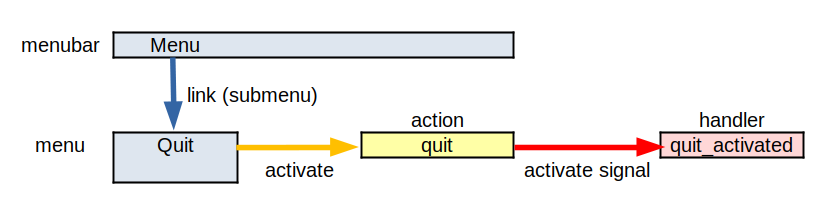
\includegraphics[width=12.555cm,height=3.285cm]{../image/menu1.png}
\caption{menu and action}
\end{figure}

\subsection{Compiling}\label{compiling}

Change your current directory to \passthrough{\lstinline!src/menu!}. Use
comp to compile \passthrough{\lstinline!menu1.c!}.

\begin{lstlisting}
$ comp menu1
$ ./a.out
\end{lstlisting}

Then, a window appears. Click on ``Menu'' on the menubar, then a menu
appears. Click on ``Quit'' menu, then the application quits.

\begin{figure}
\centering
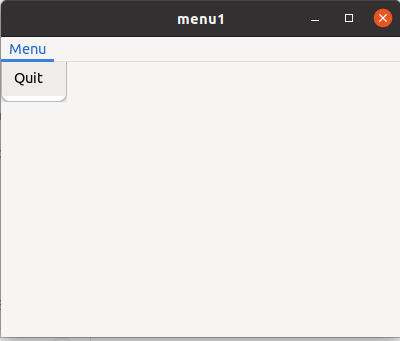
\includegraphics[width=6cm,height=5.115cm]{../image/menu1_screenshot.png}
\caption{Screenshot of menu1}
\end{figure}

\subsection{Primary and remote application
instances}\label{primary-and-remote-application-instances}

Let's try running the application twice. Use
\passthrough{\lstinline!\&!} in your shell command line, then the
application runs concurrently.

\begin{lstlisting}
$ ./a.out &
[1] 70969
$ ./a.out
$ 
\end{lstlisting}

Then, two windows appear.

\begin{itemize}
\tightlist
\item
  The first \passthrough{\lstinline!./a.out!} calls the application and
  a primary instance is created. It calls ``startup'' and ``activate''
  handlers and shows a window.
\item
  The second\passthrough{\lstinline!./a.out!} calls the the application
  again and the created instance is a remote one. It doesn't emit
  ``startup'' signal. And it activates the application but the
  ``activate'' signal is emitted on the primary instance. The remote
  instance quits.
\item
  The primary instance called ``activate'' handler. The handler creates
  a new window. It adds a menu bar to the window with
  \passthrough{\lstinline!gtk\_application\_window\_set\_show\_menubar!}
  function.
\end{itemize}

Both the windows have menu bars. And they are exactly the same. The two
windows belong to the primary instance.

If you click on the ``Quit'' menu, the application (the primary
instance) quits.

\begin{figure}
\centering
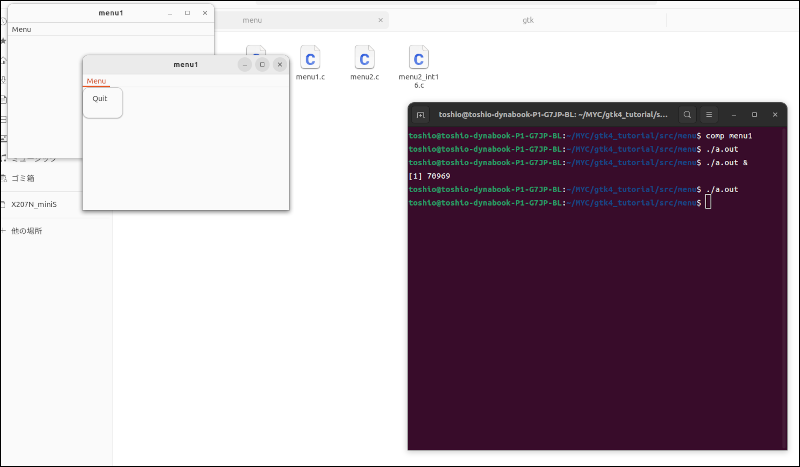
\includegraphics[width=12cm,height=7cm]{../image/menu1_two_windows.png}
\caption{menu1 -- two windows}
\end{figure}

The second execution makes a new window. However, it depends on the
``activate'' handler. If you create your window in the startup handler
and the activate handler just presents the window, no new window is
created at the second execution. For example, tfe (text file editor)
doesn't create a second window. It just creates a new notebook page.
Because its activate handler doesn't create any window but just creates
a new notebook page.

Second or more executions often happen on the desktop applications. If
you double-click the icon twice or more, the application is run multiple
times. Therefore, you need to think about your startup and activate
(open) handler carefully.

  \section{Stateful action}\label{stateful-action}

Some actions have states. The typical values of states are boolean or
string. However, other types of states are possible if you want.

Actions which have states are called stateful.

\subsection{Stateful action without a
parameter}\label{stateful-action-without-a-parameter}

Some menus are called toggle menu. For example, fullscreen menu has a
state which has two values -- fullscreen and non-fullscreen. The value
of the state is changed every time the menu is clicked. An action
corresponds to the fullscreen menu also have a state. Its value is TRUE
or FALSE and it is called boolean value. TRUE corresponds to fullscreen
and FALSE to non-fullscreen.

The following is an example code to implement a fullscreen menu except
the signal handler. The signal handler will be shown later.

\begin{lstlisting}[language=C]
GSimpleAction *act_fullscreen = g_simple_action_new_stateful ("fullscreen",
                                NULL, g_variant_new_boolean (FALSE));
g_signal_connect (act_fullscreen, "change-state", G_CALLBACK (fullscreen_changed), win);
g_action_map_add_action (G_ACTION_MAP (win), G_ACTION (act_fullscreen));
... ... ...
GMenuItem *menu_item_fullscreen = g_menu_item_new ("Full Screen", "win.fullscreen");
\end{lstlisting}

\begin{itemize}
\tightlist
\item
  \passthrough{\lstinline!act\_fullscreen!} is a GSimpleAction instance.
  It is created with
  \passthrough{\lstinline!g\_simple\_action\_new\_stateful!}. The
  function has three arguments. The first argument ``fullscreen'' is the
  name of the action. The second argument is a parameter type.
  \passthrough{\lstinline!NULL!} means the action doesn't have a
  parameter. The third argument is the initial state of the action. It
  is a GVariant value. GVariant will be explained in the next
  subsection. The function
  \passthrough{\lstinline!g\_variant\_new\_boolean (FALSE)!} returns a
  boolean type GVariant value which is \passthrough{\lstinline!FALSE!}.
  If there are two or more top level windows, each window has its own
  \passthrough{\lstinline!act\_fullscreen!} action. So, the number of
  the actions is the same as the number of the windows.
\item
  The action \passthrough{\lstinline!act\_fullscreen!} has
  ``change-state'' signal. The signal is connected to a handler
  \passthrough{\lstinline!fullscreen\_changed!}. If the fullscreen menu
  is clicked, then the corresponding action
  \passthrough{\lstinline!act\_fullscreen!} is activated. But no handler
  is connected to the ``activate'' signal. Then, the default behavior
  for boolean-stated actions with a NULL parameter type like
  \passthrough{\lstinline!act\_fullscreen!} is to toggle them via the
  ``change-state'' signal.
\item
  The action is added to the GtkWindow \passthrough{\lstinline!win!}.
  Therefore, the scope of the action is ``win''.
\item
  \passthrough{\lstinline!menu\_item\_fullscreen!} is a GMenuItem
  instance. There are two arguments. The first argument ``Full Screen''
  is the label of \passthrough{\lstinline!menu\_item\_fullscreen!}. The
  second argument is an action. The action ``win.fullscreen'' has a
  prefix ``win'' and an action name ``fullscreen''. The prefix says that
  the action belongs to the window.
\end{itemize}

\begin{lstlisting}[language=C, numbers=left]
static void
fullscreen_changed(GSimpleAction *action, GVariant *value, GtkWindow *win) {
  if (g_variant_get_boolean (value))
    gtk_window_maximize (win);
  else
    gtk_window_unmaximize (win);
  g_simple_action_set_state (action, value);
}
\end{lstlisting}

\begin{itemize}
\tightlist
\item
  The handler \passthrough{\lstinline!fullscreen\_changed!} has three
  parameters. The first parameter is the action which emits the
  ``change-state'' signal. The second parameter is the value of the new
  state of the action. The third parameter is a user data which is set
  in \passthrough{\lstinline!g\_signal\_connect!}.
\item
  If the value is boolean type and \passthrough{\lstinline!TRUE!}, then
  it maximizes the window. Otherwise it un-maximizes.
\item
  Sets the state of the action with \passthrough{\lstinline!value!}.
  Note: At this stage, that means the stage before
  \passthrough{\lstinline!g\_simple\_action\_set\_state!} is called, the
  state of the action still has the original value. So, you need to set
  the state with the new value by
  \passthrough{\lstinline!g\_simple\_action\_set\_state!}.
\end{itemize}

You can use ``activate'' signal instead of ``change-state'' signal, or
both signals. But the way above is the simplest and the best.

\subsubsection{GVariant}\label{gvariant}

GVariant is a fundamental type. It isn't a child of GObject. GVariant
can contain boolean, string or other type values. For example, the
following program assigns TRUE to \passthrough{\lstinline!value!} whose
type is GVariant.

\begin{lstlisting}[language=C]
GVariant *value = g_variant_new_boolean (TRUE);
\end{lstlisting}

Another example is:

\begin{lstlisting}[language=C]
GVariant *value2 = g_variant_new_string ("Hello");
\end{lstlisting}

\passthrough{\lstinline!value2!} is a GVariant and it has a string type
value ``Hello''. GVariant can contain other types like int16, int32,
int64, double and so on.

If you want to get the original value, use g\_variant\_get series
functions. For example, you can get the boolean value with
g\_variant\_get\_boolean.

\begin{lstlisting}[language=C]
gboolean bool = g_variant_get_boolean (value);
\end{lstlisting}

Since \passthrough{\lstinline!value!} has been created as a boolean type
GVariant with \passthrough{\lstinline!TRUE!} value,
\passthrough{\lstinline!bool!} equals \passthrough{\lstinline!TRUE!}. In
the same way, you can get a string from \passthrough{\lstinline!value2!}

\begin{lstlisting}[language=C]
const char *str = g_variant_get_string (value2, NULL);
\end{lstlisting}

The second parameter is a pointer to gsize type variable (gsize is
defined as unsigned long). If it isn't NULL, then the pointed value is
used as the length by the function. If it is NULL, nothing happens. The
returned string \passthrough{\lstinline!str!} is owned by the instance
and can't be changed or freed by the caller.

\subsection{Stateful action with a
parameter}\label{stateful-action-with-a-parameter}

Another example of stateful actions is an action corresponds to color
select menus. For example, there are three menus and each menu has red,
green or blue color respectively. They determine the background color of
a GtkLabel widget. One action is connected to the three menus. The
action has a state whose value is ``red'', ``green'' or ``blue''. The
values are string. Those colors are given to the signal handler as a
parameter.

\begin{lstlisting}[language=C]
... ... ...
GVariantType *vtype = g_variant_type_new("s");
GSimpleAction *act_color
  = g_simple_action_new_stateful ("color", vtype, g_variant_new_string ("red"));
g_variant_type_free (vtype);
GMenuItem *menu_item_red = g_menu_item_new ("Red", "app.color::red");
GMenuItem *menu_item_green = g_menu_item_new ("Green", "app.color::green");
GMenuItem *menu_item_blue = g_menu_item_new ("Blue", "app.color::blue");
g_signal_connect (act_color, "activate", G_CALLBACK (color_activated), NULL);
... ... ...
\end{lstlisting}

\begin{itemize}
\tightlist
\item
  GVariantType is a C structure and it keeps a type of GVariant. It is
  created with the function
  \passthrough{\lstinline!g\_variant\_type\_new!}. The argument of the
  function is a GVariant type string. So,
  \passthrough{\lstinline!g\_variant\_type\_new("s")!} returns a
  GVariantType structure contains a string type. The returned value,
  GVariantType structure, is owned by the caller. So, you need to free
  it when it becomes useless.
\item
  The variable \passthrough{\lstinline!act\_color!} points a
  GSimpleAction instance. It is created with
  \passthrough{\lstinline!g\_simple\_action\_new\_stateful!}. The
  function has three arguments. The first argument ``color'' is the name
  of the action. The second argument is a parameter type which is
  GVariantType. \passthrough{\lstinline!g\_variant\_type\_new("s")!}
  creates GVariantType which is a string type
  (\passthrough{\lstinline!G\_VARIANT\_TYPE\_STRING!}). The third
  argument is the initial state of the action. It is a GVariant. The
  function \passthrough{\lstinline!g\_variant\_new\_string ("red")!}
  returns a GVariant value which has the string value ``red''. GVariant
  has a reference count and
  \passthrough{\lstinline!g\_variant\_new\_...!} series functions
  returns a GVariant value with a floating reference. That means the
  caller doesn't own the value at this point. And
  \passthrough{\lstinline!g\_simple\_action\_new\_stateful!} function
  consumes the floating reference so you don't need to care about
  releasing the GVariant instance.
\item
  The GVariantType structure \passthrough{\lstinline!vtype!} is useless
  after \passthrough{\lstinline!g\_simple\_action\_new\_stateful!}. It
  is released with the function
  \passthrough{\lstinline!g\_variant\_type\_free!}.
\item
  The varable \passthrough{\lstinline!menu\_item\_red!} points a
  GMenuItem instance. The function
  \passthrough{\lstinline!g\_menu\_item\_new!} has two arguments. The
  first argument ``Red'' is the label of
  \passthrough{\lstinline!menu\_item\_red!}. The second argument is a
  detailed action. Its prefix is ``app'', action name is ``color'' and
  target is ``red''. Target is sent to the action as a parameter. The
  same goes for \passthrough{\lstinline!menu\_item\_green!} and
  \passthrough{\lstinline!menu\_item\_blue!}.
\item
  The function \passthrough{\lstinline!g\_signal\_connect!} connects the
  activate signal on the action \passthrough{\lstinline!act\_color!} and
  the handler \passthrough{\lstinline!color\_activated!}. If one of the
  three menus is clicked, then the action
  \passthrough{\lstinline!act\_color!} is activated with the target
  (parameter) which is given by the menu.
\end{itemize}

The following is the ``activate'' signal handler.

\begin{lstlisting}[language=C]
static void
color_activated(GSimpleAction *action, GVariant *parameter) {
  char *color = g_strdup_printf ("label.lb {background-color: %s;}",
                                   g_variant_get_string (parameter, NULL));
  gtk_css_provider_load_from_data (provider, color, -1);
  g_free (color);
  g_action_change_state (G_ACTION (action), parameter);
}
\end{lstlisting}

\begin{itemize}
\tightlist
\item
  The handler originally has three parameters. The third parameter is a
  user data set in the \passthrough{\lstinline!g\_signal\_connect!}
  function. But it is left out because the fourth argument of the
  \passthrough{\lstinline!g\_signal\_connect!} has been NULL. The first
  parameter is the action which emits the ``activate'' signal. The
  second parameter is the parameter, or target, given to the action. It
  is a color specified by the menu.
\item
  The variable \passthrough{\lstinline!color!} is a CSS string created
  by \passthrough{\lstinline!g\_strdup\_printf!}. The arguments of
  \passthrough{\lstinline!g\_strdup\_printf!} are the same as printf C
  standard function. The function
  \passthrough{\lstinline!g\_variant\_get\_string!} gets the string
  contained in \passthrough{\lstinline!parameter!}. The string is owned
  by the instance and you mustn't change or free it. The string
  \passthrough{\lstinline!label.lb!} is a selector. It consists of
  \passthrough{\lstinline!label!}, a node name of GtkLabel, and
  \passthrough{\lstinline!lb!} which is a class name. It selects
  GtkLabel which has \passthrough{\lstinline!lb!} class. For example,
  menus have GtkLabel to display their labels, but they don't have
  \passthrough{\lstinline!lb!} class. So, the CSS doesn't change their
  background color. The string
  \passthrough{\lstinline!\{background-color \%s\}!} makes the
  background color \passthrough{\lstinline!\%s!} to which the color from
  \passthrough{\lstinline!parameter!} is assigned.
\item
  Frees the string \passthrough{\lstinline!color!}.
\item
  Changes the state with
  \passthrough{\lstinline!g\_action\_change\_state!}.
\end{itemize}

Note: If you haven't set an ``activate'' signal handler, the signal is
forwarded to ``change-state'' signal. So, you can use ``change-state''
signal instead of ``activate'' signal. See
\passthrough{\lstinline!src/menu/menu2\_change\_state.c!}.

\subsubsection{GVariantType}\label{gvarianttype}

GVariantType gives a type of GVariant. GVariantType is created with a
type string.

\begin{itemize}
\tightlist
\item
  ``b'' means boolean type.
\item
  ``s'' means string type.
\end{itemize}

The following program is a simple example. It finally outputs the string
``s''.

\begin{lstlisting}[language=C, numbers=left]
#include <glib.h>

int
main (int argc, char **argv) {
  GVariantType *vtype = g_variant_type_new ("s");
  const char *type_string = g_variant_type_peek_string (vtype);
  g_print ("%s\n",type_string);
  g_variant_type_free (vtype);
}
\end{lstlisting}

\begin{itemize}
\tightlist
\item
  The function \passthrough{\lstinline!g\_variant\_type\_new!} creates a
  GVariantType structure. The argument ``s'' is a type string. It means
  string. The returned structure is owned by the caller. When it becomes
  useless, you need to free it with the function
  \passthrough{\lstinline!g\_variant\_type\_free!}.
\item
  The function \passthrough{\lstinline!g\_variant\_type\_peek\_string!}
  takes a peek at \passthrough{\lstinline!vtype!}. It is the string
  ``s'' given to \passthrough{\lstinline!vtype!} when it was created.
  The string is owned by the instance and the caller can't change or
  free it.
\item
  Prints the string to the terminal. You can't free
  \passthrough{\lstinline!vtype!} before
  \passthrough{\lstinline!g\_print!} because the string
  \passthrough{\lstinline!type\_string!} is owned by
  \passthrough{\lstinline!vtype!}.
\item
  Frees \passthrough{\lstinline!vtype!}.
\end{itemize}

\subsection{Example}\label{example}

The following code includes stateful actions above. This program has
menus like this:

\begin{figure}
\centering
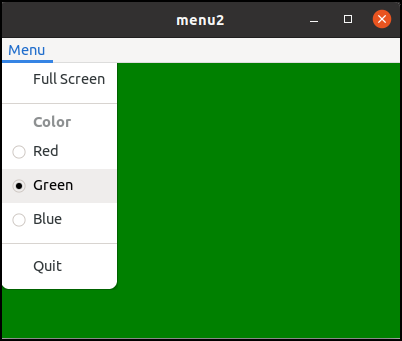
\includegraphics[width=6.03cm,height=5.115cm]{../image/menu2.png}
\caption{menu2}
\end{figure}

\begin{itemize}
\tightlist
\item
  Fullscreen menu toggles the size of the window between maximum and
  non-maximum. If the window is maximum size, which is called full
  screen, then a check mark is put before ``fullscreen'' label.
\item
  Red, green and blue menu determines the back ground color of the label
  in the window. The menus have radio buttons on the left of the menus.
  And the radio button of the selected menu turns on.
\item
  Quit menu quits the application.
\end{itemize}

The code is as follows.

\begin{lstlisting}[language=C, numbers=left]
#include <gtk/gtk.h>

/* The provider below provides application wide CSS data. */
GtkCssProvider *provider;

static void
fullscreen_changed(GSimpleAction *action, GVariant *value, GtkWindow *win) {
  if (g_variant_get_boolean (value))
    gtk_window_maximize (win);
  else
    gtk_window_unmaximize (win);
  g_simple_action_set_state (action, value);
}

static void
color_activated(GSimpleAction *action, GVariant *parameter) {
  char *color = g_strdup_printf ("label.lb {background-color: %s;}", g_variant_get_string (parameter, NULL));
  /* Change the CSS data in the provider. */
  /* Previous data is thrown away. */
  gtk_css_provider_load_from_data (provider, color, -1);
  g_free (color);
  g_action_change_state (G_ACTION (action), parameter);
}

static void
app_shutdown (GApplication *app, GtkCssProvider *provider) {
  gtk_style_context_remove_provider_for_display (gdk_display_get_default(), GTK_STYLE_PROVIDER (provider));
}

static void
app_activate (GApplication *app) {
  GtkWindow *win = GTK_WINDOW (gtk_application_window_new (GTK_APPLICATION (app)));
  gtk_window_set_title (win, "menu2");
  gtk_window_set_default_size (win, 400, 300);

  GtkWidget *lb = gtk_label_new (NULL);
  gtk_widget_add_css_class (lb, "lb"); /* the class is used by CSS Selector */
  gtk_window_set_child (win, lb);

  GSimpleAction *act_fullscreen
    = g_simple_action_new_stateful ("fullscreen", NULL, g_variant_new_boolean (FALSE));
  g_signal_connect (act_fullscreen, "change-state", G_CALLBACK (fullscreen_changed), win);
  g_action_map_add_action (G_ACTION_MAP (win), G_ACTION (act_fullscreen));

  gtk_application_window_set_show_menubar (GTK_APPLICATION_WINDOW (win), TRUE);

  gtk_window_present (win);
}

static void
app_startup (GApplication *app) {
  GVariantType *vtype = g_variant_type_new("s");
  GSimpleAction *act_color
    = g_simple_action_new_stateful ("color", vtype, g_variant_new_string ("red"));
  g_variant_type_free (vtype);
  GSimpleAction *act_quit
    = g_simple_action_new ("quit", NULL);
  g_signal_connect (act_color, "activate", G_CALLBACK (color_activated), NULL);
  g_signal_connect_swapped (act_quit, "activate", G_CALLBACK (g_application_quit), app);
  g_action_map_add_action (G_ACTION_MAP (app), G_ACTION (act_color));
  g_action_map_add_action (G_ACTION_MAP (app), G_ACTION (act_quit));

  GMenu *menubar = g_menu_new ();
  GMenu *menu = g_menu_new ();
  GMenu *section1 = g_menu_new ();
  GMenu *section2 = g_menu_new ();
  GMenu *section3 = g_menu_new ();
  GMenuItem *menu_item_fullscreen = g_menu_item_new ("Full Screen", "win.fullscreen");
  GMenuItem *menu_item_red = g_menu_item_new ("Red", "app.color::red");
  GMenuItem *menu_item_green = g_menu_item_new ("Green", "app.color::green");
  GMenuItem *menu_item_blue = g_menu_item_new ("Blue", "app.color::blue");
  GMenuItem *menu_item_quit = g_menu_item_new ("Quit", "app.quit");

  g_menu_append_item (section1, menu_item_fullscreen);
  g_menu_append_item (section2, menu_item_red);
  g_menu_append_item (section2, menu_item_green);
  g_menu_append_item (section2, menu_item_blue);
  g_menu_append_item (section3, menu_item_quit);
  g_object_unref (menu_item_red);
  g_object_unref (menu_item_green);
  g_object_unref (menu_item_blue);
  g_object_unref (menu_item_fullscreen);
  g_object_unref (menu_item_quit);

  g_menu_append_section (menu, NULL, G_MENU_MODEL (section1));
  g_menu_append_section (menu, "Color", G_MENU_MODEL (section2));
  g_menu_append_section (menu, NULL, G_MENU_MODEL (section3));
  g_menu_append_submenu (menubar, "Menu", G_MENU_MODEL (menu));
  g_object_unref (section1);
  g_object_unref (section2);
  g_object_unref (section3);
  g_object_unref (menu);

  gtk_application_set_menubar (GTK_APPLICATION (app), G_MENU_MODEL (menubar));

  provider = gtk_css_provider_new ();
  /* Initialize the css data */
  gtk_css_provider_load_from_data (provider, "label.lb {background-color: red;}", -1);
  /* Add CSS to the default GdkDisplay. */
  gtk_style_context_add_provider_for_display (gdk_display_get_default (),
        GTK_STYLE_PROVIDER (provider), GTK_STYLE_PROVIDER_PRIORITY_APPLICATION);
  g_signal_connect (app, "shutdown", G_CALLBACK (app_shutdown), provider);
  g_object_unref (provider); /* release provider, but it's still alive because the display owns it */
}

#define APPLICATION_ID "com.github.ToshioCP.menu2"

int
main (int argc, char **argv) {
  GtkApplication *app;
  int stat;

  app = gtk_application_new (APPLICATION_ID, G_APPLICATION_DEFAULT_FLAGS);
  g_signal_connect (app, "startup", G_CALLBACK (app_startup), NULL);
  g_signal_connect (app, "activate", G_CALLBACK (app_activate), NULL);

  stat =g_application_run (G_APPLICATION (app), argc, argv);
  g_object_unref (app);
  return stat;
}
\end{lstlisting}

\begin{itemize}
\tightlist
\item
  6-23: Action signal handlers.
\item
  25-28: The handler \passthrough{\lstinline!app\_shutdown!} is called
  when the application quits. It removes the provider from the display.
\item
  30-48: An activate signal handler.
\item
  32-34: A new window is created and assigned to
  \passthrough{\lstinline!win!}. Its title and default size are set to
  ``menu2'' and 400x300 respectively.
\item
  36-38: A new label is created and assigned to
  \passthrough{\lstinline!lb!} The label is given a CSS class ``lb''. It
  is added to \passthrough{\lstinline!win!} as a child.
\item
  40-43: A toggle action is created and assigned to
  \passthrough{\lstinline!act\_fullscreen!}. It's connected to the
  signal handler \passthrough{\lstinline!fullscreen\_changed!}. It's
  added to the window, so the action scope is ``win''. So, if there are
  two or more windows, the actions are created two or more.
\item
  45: The function
  \passthrough{\lstinline!gtk\_application\_window\_set\_show\_menubar!}
  adds a menubar to the window.
\item
  47: Shows the window.
\item
  50-104: A startup signal handler.
\item
  52-61: Two actions \passthrough{\lstinline!act\_color!} and
  \passthrough{\lstinline!act\_quit!} are created. These actions exists
  only one because the startup handler is called once. They are
  connected to their handlers and added to the application. Their scopes
  are ``app''.
\item
  63-92: Menus are built.
\item
  94: The menubar is added to the application.
\item
  96-103: A CSS provider is created with the CSS data and added to the
  default display. The ``shutdown'' signal on the application is
  connected to a handler ``app\_shutdown''. So, the provider is removed
  from the display and freed when the application quits.
\end{itemize}

\subsection{Compile}\label{compile}

Change your current directory to \passthrough{\lstinline!src/menu!}.

\begin{lstlisting}
$ comp menu2
$./a.out
\end{lstlisting}

Then, you will see a window and the background color of the content is
red. You can change the size to maximum and change back to the original
size. You can change the background color to green or blue.

If you run the second application during the first application is
running, another window will appear in the same screen. Both of the
window have the same background color. Because the
\passthrough{\lstinline!act\_color!} action has ``app'' scope and the
CSS is applied to the default display shared by the windows.

\begin{lstlisting}
$ ./a.out & # Run the first application
[1] 82113
$ ./a.out # Run the second application
$ 
\end{lstlisting}

  \section{Ui file for menu and action
entries}\label{ui-file-for-menu-and-action-entries}

\subsection{Ui file for menu}\label{ui-file-for-menu}

You may have thought that building menus was really bothersome. Yes, the
program was complicated and it needs lots of time to code them. The
situation is similar to building widgets. When we built widgets, using
ui file was a good way to avoid such complication. The same goes for
menus.

The ui file for menus has interface and menu tags. The file starts and
ends with interface tags.

\begin{lstlisting}[language=XML]
<interface>
  <menu id="menubar">
  </menu>
</interface>
\end{lstlisting}

\passthrough{\lstinline!menu!} tag corresponds to GMenu object.
\passthrough{\lstinline!id!} attribute defines the name of the object.
It will be referred by GtkBuilder.

\begin{lstlisting}[language=XML]
<submenu>
  <attribute name="label">File</attribute>
    <item>
      <attribute name="label">New</attribute>
      <attribute name="action">win.new</attribute>
    </item>
</submenu>
\end{lstlisting}

\passthrough{\lstinline!item!} tag corresponds to an item in the GMenu
which has the same structure as GMenuItem. The item above has a label
attribute. Its value is ``New''. The item also has an action attribute
and its value is ``win.new''. ``win'' is a prefix and ``new'' is an
action name. \passthrough{\lstinline!submenu!} tag corresponds to both
GMenuItem and GMenu. The GMenuItem has a link to GMenu.

The ui file above can be described as follows.

\begin{lstlisting}[language=XML]
<item>
  <attribute name="label">File</attribute>
    <link name="submenu">
      <item>
        <attribute name="label">New</attribute>
        <attribute name="action">win.new</attribute>
      </item>
    </link>
</item>
\end{lstlisting}

\passthrough{\lstinline!link!} tag expresses the link to submenu. And at
the same time it also expresses the submenu itself. This file
illustrates the relationship between the menus and items better than the
prior ui file. But \passthrough{\lstinline!submenu!} tag is simple and
easy to understand. So, we usually prefer the former ui style.

For further information, see
\href{https://docs.gtk.org/gtk4/class.PopoverMenu.html\#menu-models}{GTK
4 API reference -- PopoverMenu}.

The following is a screenshot of the sample program
\passthrough{\lstinline!menu3!}. It is located in the directory
src/menu3.

\begin{figure}
\centering
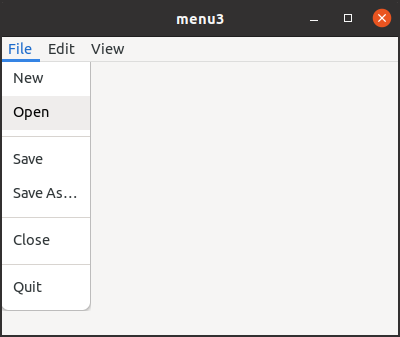
\includegraphics[width=6cm,height=5.055cm]{../image/menu3.png}
\caption{menu3}
\end{figure}

The following is the ui file for \passthrough{\lstinline!menu3!}.

\begin{lstlisting}[language=XML, numbers=left]
<?xml version="1.0" encoding="UTF-8"?>
<interface>
  <menu id="menubar">
    <submenu>
      <attribute name="label">File</attribute>
      <section>
        <item>
          <attribute name="label">New</attribute>
          <attribute name="action">app.new</attribute>
        </item>
        <item>
          <attribute name="label">Open</attribute>
          <attribute name="action">app.open</attribute>
        </item>
      </section>
      <section>
        <item>
          <attribute name="label">Save</attribute>
          <attribute name="action">win.save</attribute>
        </item>
        <item>
          <attribute name="label">Save As…</attribute>
          <attribute name="action">win.saveas</attribute>
        </item>
      </section>
      <section>
        <item>
          <attribute name="label">Close</attribute>
          <attribute name="action">win.close</attribute>
        </item>
      </section>
      <section>
        <item>
          <attribute name="label">Quit</attribute>
          <attribute name="action">app.quit</attribute>
        </item>
      </section>
    </submenu>
    <submenu>
      <attribute name="label">Edit</attribute>
      <section>
        <item>
          <attribute name="label">Cut</attribute>
          <attribute name="action">app.cut</attribute>
        </item>
        <item>
          <attribute name="label">Copy</attribute>
          <attribute name="action">app.copy</attribute>
        </item>
        <item>
          <attribute name="label">Paste</attribute>
          <attribute name="action">app.paste</attribute>
        </item>
      </section>
      <section>
        <item>
          <attribute name="label">Select All</attribute>
          <attribute name="action">app.selectall</attribute>
        </item>
      </section>
    </submenu>
    <submenu>
      <attribute name="label">View</attribute>
      <section>
        <item>
          <attribute name="label">Full Screen</attribute>
          <attribute name="action">win.fullscreen</attribute>
        </item>
      </section>
    </submenu>
  </menu>
</interface>
\end{lstlisting}

The ui file is converted to the resource by the resource compiler
\passthrough{\lstinline!glib-compile-resouces!} with xml file.

\begin{lstlisting}[language=XML, numbers=left]
<?xml version="1.0" encoding="UTF-8"?>
<gresources>
  <gresource prefix="/com/github/ToshioCP/menu3">
    <file>menu3.ui</file>
  </gresource>
</gresources>
\end{lstlisting}

GtkBuilder builds menus from the resource.

\begin{lstlisting}[language=C]
GtkBuilder *builder = gtk_builder_new_from_resource ("/com/github/ToshioCP/menu3/menu3.ui");
GMenuModel *menubar = G_MENU_MODEL (gtk_builder_get_object (builder, "menubar"));

gtk_application_set_menubar (GTK_APPLICATION (app), menubar);
g_object_unref (builder);
\end{lstlisting}

The builder instance is freed after the GMenuModel
\passthrough{\lstinline!menubar!} is inserted to the application. If you
do it before the insertion, bad thing will happen -- your computer might
freeze. It is because you don't own the
\passthrough{\lstinline!menubar!} instance. The function
\passthrough{\lstinline!gtk\_builder\_get\_object!} just returns the
pointer to \passthrough{\lstinline!menubar!} and doesn't increase the
reference count of \passthrough{\lstinline!menubar!}. So, if you
released \passthrough{\lstinline!bulder!} before
\passthrough{\lstinline!gtk\_application\_set\_menubar!},
\passthrough{\lstinline!builder!} would be destroyed and
\passthrough{\lstinline!menubar!} as well.

\subsection{Action entry}\label{action-entry}

The coding for building actions and signal handlers is bothersome work
as well. Therefore, it should be automated. You can implement them
easily with GActionEntry structure and
\passthrough{\lstinline!g\_action\_map\_add\_action\_entries!} function.

GActionEntry contains action name, signal handlers, parameter and state.

\begin{lstlisting}[language=C]
typedef struct _GActionEntry GActionEntry;

struct _GActionEntry
{
  /* action name */
  const char *name;
  /* activate handler */
  void (* activate) (GSimpleAction *action, GVariant *parameter, gpointer user_data);
  /* the type of the parameter given as a single GVariant type string */
  const char *parameter_type;
  /* initial state given in GVariant text format */
  const char *state;
  /* change-state handler */
  void (* change_state) (GSimpleAction *action, GVariant *value, gpointer user_data);
  /*< private >*/
  gsize padding[3];
};
\end{lstlisting}

For example, the actions in the previous section are:

\begin{lstlisting}[language=C]
{ "fullscreen", NULL, NULL, "false", fullscreen_changed }
{ "color", color_activated, "s", "'red'", NULL }
{ "quit", quit_activated, NULL, NULL, NULL },
\end{lstlisting}

\begin{itemize}
\tightlist
\item
  Fullscreen action is stateful, but doesn't have parameters. So, the
  third element (parameter type) is NULL.
  \href{https://docs.gtk.org/glib/gvariant-text.html}{GVariant text
  format} provides ``true'' and ``false'' as boolean GVariant values.
  The initial state of the action is false (the fourth element). It
  doesn't have activate handler, so the second element is NULL. Instead,
  it has change-state handler. The fifth element
  \passthrough{\lstinline!fullscreen\_changed!} is the handler.
\item
  Color action is stateful and has a parameter. The parameter type is
  string.
  \href{https://docs.gtk.org/glib/gvariant-format-strings.html}{GVariant
  format strings} provides string formats to represent GVariant types.
  The third element ``s'' means GVariant string type. GVariant text
  format defines that strings are surrounded by single or double quotes.
  So, the string red is `red' or ``red''. The fourth element is
  \passthrough{\lstinline!"'red'"!}, which is a C string format and the
  string is `red'. You can write \passthrough{\lstinline!"\\"red\\""!}
  instead. The second element \passthrough{\lstinline!color\_activated!}
  is the activate handler. The action doesn't have change-state handler,
  so the fifth element is NULL.
\item
  Quit action is non-stateful and has no parameter. So, the third and
  fourth elements are NULL. The second element
  \passthrough{\lstinline!quit\_activated!} is the activate handler. The
  action doesn't have change-state handler, so the fifth element is
  NULL.
\end{itemize}

The function
\passthrough{\lstinline!g\_action\_map\_add\_action\_entries!} does
everything to create GSimpleAction instances and add them to a
GActionMap (an application or window).

\begin{lstlisting}[language=C]
const GActionEntry app_entries[] = {
  { "color", color_activated, "s", "'red'", NULL },
  { "quit", quit_activated, NULL, NULL, NULL }
};
g_action_map_add_action_entries (G_ACTION_MAP (app), app_entries,
                                 G_N_ELEMENTS (app_entries), app);
\end{lstlisting}

The code above does:

\begin{itemize}
\tightlist
\item
  Builds the ``color'' and ``quit'' actions
\item
  Connects the action and the ``activate'' signal handlers
  (\passthrough{\lstinline!color\_activated!} and
  \passthrough{\lstinline!quit\_activated!}).
\item
  Adds the actions to the action map \passthrough{\lstinline!app!}.
\end{itemize}

The same goes for the other action.

\begin{lstlisting}[language=C]
const GActionEntry win_entries[] = {
  { "fullscreen", NULL, NULL, "false", fullscreen_changed }
};
g_action_map_add_action_entries (G_ACTION_MAP (win), win_entries,
                                 G_N_ELEMENTS (win_entries), win);
\end{lstlisting}

The code above does:

\begin{itemize}
\tightlist
\item
  Builds the ``fullscreen'' action.
\item
  Connects the action and the signal handler
  \passthrough{\lstinline!fullscreen\_changed!}
\item
  Its initial state is set to false.
\item
  Adds the action to the action map \passthrough{\lstinline!win!}.
\end{itemize}

\subsection{Example}\label{example}

Source files are \passthrough{\lstinline!menu3.c!},
\passthrough{\lstinline!menu3.ui!},
\passthrough{\lstinline!menu3.gresource.xml!} and
\passthrough{\lstinline!meson.build!}. They are in the directory
src/menu3. The following are \passthrough{\lstinline!menu3.c!} and
\passthrough{\lstinline!meson.build!}.

\begin{lstlisting}[language=C, numbers=left]
#include <gtk/gtk.h>

static void
new_activated (GSimpleAction *action, GVariant *parameter, gpointer user_data) {
}

static void
open_activated (GSimpleAction *action, GVariant *parameter, gpointer user_data) {
}

static void
save_activated (GSimpleAction *action, GVariant *parameter, gpointer user_data) {
}

static void
saveas_activated (GSimpleAction *action, GVariant *parameter, gpointer user_data) {
}

static void
close_activated (GSimpleAction *action, GVariant *parameter, gpointer user_data) {
  GtkWindow *win = GTK_WINDOW (user_data);

  gtk_window_destroy (win);
}

static void
cut_activated (GSimpleAction *action, GVariant *parameter, gpointer user_data) {
}

static void
copy_activated (GSimpleAction *action, GVariant *parameter, gpointer user_data) {
}

static void
paste_activated (GSimpleAction *action, GVariant *parameter, gpointer user_data) {
}

static void
selectall_activated (GSimpleAction *action, GVariant *parameter, gpointer user_data) {
}

static void
fullscreen_changed (GSimpleAction *action, GVariant *state, gpointer user_data) {
  GtkWindow *win = GTK_WINDOW (user_data);

  if (g_variant_get_boolean (state))
    gtk_window_maximize (win);
  else
    gtk_window_unmaximize (win);
  g_simple_action_set_state (action, state);
}

static void
quit_activated (GSimpleAction *action, GVariant *parameter, gpointer user_data) {
  GApplication *app = G_APPLICATION (user_data);

  g_application_quit (app);
}

static void
app_activate (GApplication *app) {
  GtkWidget *win = gtk_application_window_new (GTK_APPLICATION (app));

  const GActionEntry win_entries[] = {
    { "save", save_activated, NULL, NULL, NULL },
    { "saveas", saveas_activated, NULL, NULL, NULL },
    { "close", close_activated, NULL, NULL, NULL },
    { "fullscreen", NULL, NULL, "false", fullscreen_changed }
  };
  g_action_map_add_action_entries (G_ACTION_MAP (win), win_entries, G_N_ELEMENTS (win_entries), win);

  gtk_application_window_set_show_menubar (GTK_APPLICATION_WINDOW (win), TRUE);

  gtk_window_set_title (GTK_WINDOW (win), "menu3");
  gtk_window_set_default_size (GTK_WINDOW (win), 400, 300);
  gtk_window_present (GTK_WINDOW (win));
}

static void
app_startup (GApplication *app) {
  GtkBuilder *builder = gtk_builder_new_from_resource ("/com/github/ToshioCP/menu3/menu3.ui");
  GMenuModel *menubar = G_MENU_MODEL (gtk_builder_get_object (builder, "menubar"));

  gtk_application_set_menubar (GTK_APPLICATION (app), menubar);
  g_object_unref (builder);

  const GActionEntry app_entries[] = {
    { "new", new_activated, NULL, NULL, NULL },
    { "open", open_activated, NULL, NULL, NULL },
    { "cut", cut_activated, NULL, NULL, NULL },
    { "copy", copy_activated, NULL, NULL, NULL },
    { "paste", paste_activated, NULL, NULL, NULL },
    { "selectall", selectall_activated, NULL, NULL, NULL },
    { "quit", quit_activated, NULL, NULL, NULL }
  };
  g_action_map_add_action_entries (G_ACTION_MAP (app), app_entries, G_N_ELEMENTS (app_entries), app);
}

#define APPLICATION_ID "com.github.ToshioCP.menu3"

int
main (int argc, char **argv) {
  GtkApplication *app;
  int stat;

  app = gtk_application_new (APPLICATION_ID, G_APPLICATION_DEFAULT_FLAGS);
  g_signal_connect (app, "startup", G_CALLBACK (app_startup), NULL);
  g_signal_connect (app, "activate", G_CALLBACK (app_activate), NULL);

  stat =g_application_run (G_APPLICATION (app), argc, argv);
  g_object_unref (app);
  return stat;
}
\end{lstlisting}

meson.build

\begin{lstlisting}[numbers=left]
project('menu3', 'c')

gtkdep = dependency('gtk4')

gnome=import('gnome')
resources = gnome.compile_resources('resources','menu3.gresource.xml')

sourcefiles=files('menu3.c')

executable('menu3', sourcefiles, resources, dependencies: gtkdep)
\end{lstlisting}

Action handlers need to follow the following format.

\begin{lstlisting}[language=C]
static void
handler (GSimpleAction *action_name, GVariant *parameter, gpointer user_data) { ... ... ... }
\end{lstlisting}

You can't write, for example, ``GApplication *app'' instead of
``gpointer user\_data''. Because
\passthrough{\lstinline!g\_action\_map\_add\_action\_entries!} expects
that handlers follow the format above.

There are \passthrough{\lstinline!menu2\_ui.c!} and
\passthrough{\lstinline!menu2.ui!} under the
\passthrough{\lstinline!menu!} directory. They are other examples to
show menu ui file and
\passthrough{\lstinline!g\_action\_map\_add\_action\_entries!}. It
includes a stateful action with parameters.

\begin{lstlisting}[language=XML]
<item>
  <attribute name="label">Red</attribute>
  <attribute name="action">app.color</attribute>
  <attribute name="target">red</attribute>
</item>
\end{lstlisting}

Action name and target are separated like this. Action attribute
includes prefix and name only. You can't write like
\passthrough{\lstinline!<attribute name="action">app.color::red</attribute>!}.

  \section{Composite widgets and alert
dialog}\label{composite-widgets-and-alert-dialog}

The source files are in the
\href{https://github.com/ToshioCP/Gtk4-tutorial}{Gtk4 tutorial GitHub
repository}. Download it and see \passthrough{\lstinline!src/tfe6!}
directory.

\subsection{An outline of new Tfe text
editor}\label{an-outline-of-new-tfe-text-editor}

Tfe text editor will be restructured. The program is divided into six
parts.

\begin{itemize}
\tightlist
\item
  Main program: the C main function.
\item
  TfeApplication object: It is like GtkApplication but keeps GSettings
  and CSS Provider.
\item
  TfeWindow object: It is a window with buttons and a notebook.
\item
  TfePref object: A preference dialog.
\item
  TfeAlert object: An alert dialog.
\item
  pdf2css.h and pdf2css.c: Font and CSS utility functions.
\end{itemize}

This section describes TfeAlert. Others will be explained in the
following sections.

\subsection{Composite widgets}\label{composite-widgets}

The alert dialog is like this:

\begin{figure}
\centering
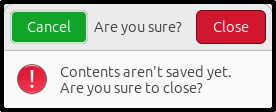
\includegraphics[width=4.2cm,height=1.7cm]{../image/alert.png}
\caption{Alert dialog}
\end{figure}

Tfe uses it when a user quits the application or closes a notebook
without saving data to files.

The dialog has a title, buttons, an icon and a message. Therefore, it
consists of several widgets. Such dialog is called a composite widget.

Composite widgets are defined with template XMLs. The class is built in
the class initialization function and the instances are built and
desposed by the following functions.

\begin{itemize}
\tightlist
\item
  gtk\_widget\_init\_template
\item
  gtk\_widget\_dispose\_template
\end{itemize}

TfeAlert is a good example to know composite widgets. It is defined with
the three files.

\begin{itemize}
\tightlist
\item
  tfealert.ui: XML file
\item
  tfealert.h: Header file
\item
  tfealert.c: C program file
\end{itemize}

\subsection{The XML file}\label{the-xml-file}

A template tag is used in a composite widget XML.

\begin{lstlisting}[language=XML, numbers=left]
<?xml version="1.0" encoding="UTF-8"?>
<interface>
  <template class="TfeAlert" parent="GtkWindow">
    <property name="resizable">FALSE</property>
    <property name="modal">TRUE</property>
    <property name="titlebar">
      <object class="GtkHeaderBar">
        <property name="show-title-buttons">FALSE</property>
        <property name="title-widget">
          <object class="GtkLabel" id="lb_title">
            <property name="label">Are you sure?</property>
            <property name="single-line-mode">True</property>
          </object>
        </property>
        <child type="start">
          <object class="GtkButton" id="btn_cancel">
            <property name="label">Cancel</property>
            <style>
              <class name="suggested-action"/>
            </style>
            <signal name="clicked" handler="cancel_cb" swapped="TRUE" object="TfeAlert"></signal>
          </object>
        </child>
        <child type="end">
          <object class="GtkButton" id="btn_accept">
            <property name="label">Close</property>
            <style>
              <class name="destructive-action"/>
            </style>
            <signal name="clicked" handler="accept_cb" swapped="TRUE" object="TfeAlert"></signal>
          </object>
        </child>
      </object>
    </property>
    <child>
      <object class="GtkBox">
        <property name="orientation">GTK_ORIENTATION_HORIZONTAL</property>
        <property name="spacing">12</property>
        <property name="margin-top">12</property>
        <property name="margin-bottom">12</property>
        <property name="margin-start">12</property>
        <property name="margin-end">12</property>
        <child>
          <object class="GtkImage">
            <property name="icon-name">dialog-warning</property>
            <property name="icon-size">GTK_ICON_SIZE_LARGE</property>
          </object>
        </child>
        <child>
          <object class="GtkLabel" id="lb_message">
          </object>
        </child>
      </object>
    </child>
  </template>
</interface>
\end{lstlisting}

\begin{itemize}
\tightlist
\item
  3: A template tag defines a composite widget. The class attribute
  tells the class name of the composite widget. The parent attribute
  tells the parent class of the composite widget. So, TfeAlert is a
  child class of GtkWindow. A parent attribute is an option and you can
  leave it out. But it is recommended to write it in the template tag.
\item
  4-6: Its three properties are defined. These properties are inherited
  from GtkWindow. The titlebar property has a widget for a custom title
  bar. The typical widget is GtkHeaderBar.
\item
  8: If the property ``show-title-buttons'' is TRUE, the title buttons
  like close, minimize and maximize are shown. Otherwise it is not
  shown. The TfeAlert object is not resizable. It is closed when either
  of the two buttons, cancel or accept, is clicked. Therefore the title
  buttons are not necessary and this property is set to FALSE.
\item
  9-14: The bar has a title, which is a GtkLabel widget. The default
  title is ``Are you sure?'' but it can be replaced by an instance
  method.
\item
  15-32: The bar has two buttons, cancel and accept. The cancel button
  is on the left so the child tag has
  \passthrough{\lstinline!type="start"!} attribute. The accept button is
  on the right so the child tag has \passthrough{\lstinline!type="end"!}
  attribute. The dialog is shown when the user clicked the close button
  or the quit menu without saving the data. Therefore, it is safer for
  the user to click on the cancel button of the alert dialog. So, the
  cancel button has a ``suggested-action'' CSS class. Ubuntu colors the
  button green but the color can be blue or other appropriate one
  defined by the system. In the same way the accept button has a
  ``destructive-action'' CSS class and is colored red. Two buttons have
  signals which are defined by the signal tags.
\item
  35-54: A horizontal box has an image icon and a label.
\item
  44-47: The GtkImage widget displays an image. The ``icon-name''
  property is an icon name in the icon theme. The theme depends on your
  system. You can check it with an icon browser.
\end{itemize}

\begin{lstlisting}
$ gtk4-icon-browser
\end{lstlisting}

The ``dialog-warning'' icon is something like this.

\begin{figure}
\centering

\includegraphics[width=4.19cm,height=1.62cm]{../image/dialog_warning.png}
\caption{dialog-warning icon is like \ldots{}}
\end{figure}

These are made by my hand. The real image on the alert dialog is nicer.

It is possible to define the alert widget as a child of GtkDialog. But
GtkDialog is deprecated since GTK version 4.10. And users should use
GtkWindow instead of GtkDialog.

\subsection{The header file}\label{the-header-file}

The header file is similar to the one of TfeTextView.

\begin{lstlisting}[language=C, numbers=left]
#pragma once

#include <gtk/gtk.h>

#define TFE_TYPE_ALERT tfe_alert_get_type ()
G_DECLARE_FINAL_TYPE (TfeAlert, tfe_alert, TFE, ALERT, GtkWindow)

/* "response" signal id */
enum TfeAlertResponseType
{
  TFE_ALERT_RESPONSE_ACCEPT,
  TFE_ALERT_RESPONSE_CANCEL
};

const char *
tfe_alert_get_title (TfeAlert *alert);

const char *
tfe_alert_get_message (TfeAlert *alert);

const char *
tfe_alert_get_button_label (TfeAlert *alert);

void
tfe_alert_set_title (TfeAlert *alert, const char *title);

void
tfe_alert_set_message (TfeAlert *alert, const char *message);

void
tfe_alert_set_button_label (TfeAlert *alert, const char *btn_label);

GtkWidget *
tfe_alert_new (void);

GtkWidget *
tfe_alert_new_with_data (const char *title, const char *message, const char* btn_label);
\end{lstlisting}

\begin{itemize}
\tightlist
\item
  5-6: These two lines are always needed to define a new object.
  \passthrough{\lstinline!TFE\_TYPE\_ALERT!} is the type of TfeAlert
  object and it is a macro expanded into
  \passthrough{\lstinline!tfe\_alert\_get\_type ()!}.
  G\_DECLARE\_FINAL\_TYPE macro is expanded into:

  \begin{itemize}
  \tightlist
  \item
    The declaration of the function
    \passthrough{\lstinline!tfe\_alert\_get\_type!}
  \item
    \passthrough{\lstinline!TfeAlert!} is defined as a typedef of
    \passthrough{\lstinline!struct \_TfeAlert!}, which is defined in the
    C file.
  \item
    \passthrough{\lstinline!TFE\_ALERT!} and
    \passthrough{\lstinline!TFE\_IS\_ALERT!} macro is defined as a cast
    and type check function.
  \item
    \passthrough{\lstinline!TfeAlertClass!} structure is defined as a
    final class.
  \end{itemize}
\item
  8-13: The TfeAlert class has a ``response'' signal. It has a parameter
  and the parameter type is defined as a
  \passthrough{\lstinline!TfeAlertResponseType!} enumerative constant.
\item
  15-31: Getter and setter methods.
\item
  33-37: Functions to create a instance. The function
  \passthrough{\lstinline!tfe\_alert\_new\_with\_data!} is a convenience
  function, which creates an instance and sets data at once.
\end{itemize}

\subsection{The C file}\label{the-c-file}

\subsubsection{Functions for composite
widgets}\label{functions-for-composite-widgets}

The following codes are extracted from
\passthrough{\lstinline!tfealert.c!}.

\begin{lstlisting}[language=C]
#include <gtk/gtk.h>
#include "tfealert.h"

struct _TfeAlert {
  GtkWindow parent;
  GtkLabel *lb_title;
  GtkLabel *lb_message;
  GtkButton *btn_accept;
  GtkButton *btn_cancel;
};

G_DEFINE_FINAL_TYPE (TfeAlert, tfe_alert, GTK_TYPE_WINDOW);

static void
cancel_cb (TfeAlert *alert) {
  ... ... ...
}

static void
accept_cb (TfeAlert *alert) {
  ... ... ...
}

static void
tfe_alert_dispose (GObject *gobject) { // gobject is actually a TfeAlert instance.
  gtk_widget_dispose_template (GTK_WIDGET (gobject), TFE_TYPE_ALERT);
  G_OBJECT_CLASS (tfe_alert_parent_class)->dispose (gobject);
}

static void
tfe_alert_init (TfeAlert *alert) {
  gtk_widget_init_template (GTK_WIDGET (alert));
}

static void
tfe_alert_class_init (TfeAlertClass *class) {
  G_OBJECT_CLASS (class)->dispose = tfe_alert_dispose;
  gtk_widget_class_set_template_from_resource (GTK_WIDGET_CLASS (class), "/com/github/ToshioCP/tfe/tfealert.ui");
  gtk_widget_class_bind_template_child (GTK_WIDGET_CLASS (class), TfeAlert, lb_title);
  gtk_widget_class_bind_template_child (GTK_WIDGET_CLASS (class), TfeAlert, lb_message);
  gtk_widget_class_bind_template_child (GTK_WIDGET_CLASS (class), TfeAlert, btn_accept);
  gtk_widget_class_bind_template_child (GTK_WIDGET_CLASS (class), TfeAlert, btn_cancel);
  gtk_widget_class_bind_template_callback (GTK_WIDGET_CLASS (class), cancel_cb);
  gtk_widget_class_bind_template_callback (GTK_WIDGET_CLASS (class), accept_cb);
  ... ... ...
}

GtkWidget *
tfe_alert_new (void) {
  return GTK_WIDGET (g_object_new (TFE_TYPE_ALERT, NULL));
}
\end{lstlisting}

\begin{itemize}
\tightlist
\item
  The macro \passthrough{\lstinline!G\_DEFINE\_FINAL\_TYPE!} is
  available since GLib version 2.70. It is used only for a final type
  class. You can use \passthrough{\lstinline!G\_DEFINE\_TYPE!} macro
  instead. They are expanded into:

  \begin{itemize}
  \tightlist
  \item
    The declaration of the functions
    \passthrough{\lstinline!tfe\_alert\_init!} and
    \passthrough{\lstinline!tfe\_alert\_class\_init!}. They are defined
    in the following part of the C program.
  \item
    The definition of the variable
    \passthrough{\lstinline!tfe\_alert\_parent\_class!}.
  \item
    The definition of the function
    \passthrough{\lstinline!tfe\_alert\_get\_type!}.
  \end{itemize}
\item
  The names of the members of \passthrough{\lstinline!\_TfeAlert!},
  which are \passthrough{\lstinline!lb\_title!},
  \passthrough{\lstinline!lb\_message!},
  \passthrough{\lstinline!btn\_accept!} and
  \passthrough{\lstinline!btn\_cancel!}, must be the same as the id
  attribute in the XML file \passthrough{\lstinline!tfealert.ui!}.
\item
  The function \passthrough{\lstinline!tfe\_alert\_class\_init!}
  initializes the composite widget class.

  \begin{itemize}
  \tightlist
  \item
    The function
    \passthrough{\lstinline!gtk\_widget\_class\_set\_template\_from\_resource!}
    sets the template of the class. The template is built from the XML
    resource ``tfealert.ui''. At this moment no instance is created. It
    just makes the class recognize the structure of the object. That's
    why the top level tag is not object but template in the XML file.
  \item
    The function macro
    \passthrough{\lstinline!gtk\_widget\_class\_bind\_template\_child!}
    connects the member of TfeAlert and the object class in the
    template. So, for example, you can access to
    \passthrough{\lstinline!lb\_title!} GtkLabel instance via
    \passthrough{\lstinline!alert->lb\_title!} where
    \passthrough{\lstinline!alert!} is an instance of TfeAlert class.
  \item
    The function
    \passthrough{\lstinline!gtk\_widget\_class\_bind\_template\_callback!}
    connects the callback function and the
    \passthrough{\lstinline!handler!} attribute of the signal tag in the
    XML. For example, the ``clicked'' signal on the cancel button has a
    handler named ``cancel\_cb'' in the signal tag. And the function
    \passthrough{\lstinline!cancel\_cb!} exists in the C file above.
    These two are connected so when the signal is emitted the function
    \passthrough{\lstinline!cancel\_cb!} is called. You can add
    \passthrough{\lstinline!static!} storage class to the callback
    function thanks to this connection.
  \end{itemize}
\item
  The function \passthrough{\lstinline!tfe\_alert\_init!} initializes
  the newly created instance. You need to call
  \passthrough{\lstinline!gtk\_widget\_init\_template!} to create and
  initialize the child widgets in the template.
\item
  The function \passthrough{\lstinline!tfe\_alert\_despose!} releases
  objects. The function
  \passthrough{\lstinline!gtk\_widget\_despose\_template!} clears the
  template children.
\item
  The function \passthrough{\lstinline!tfe\_alert\_new!} creates the
  composite widget TfeAlert instance. It creates not only TfeAlert
  itself but also all the child widgets that the composite widget has.
\end{itemize}

\subsubsection{Other functions}\label{other-functions}

The following is the full codes of \passthrough{\lstinline!tfealert.c!}.

\begin{lstlisting}[language=C, numbers=left]
#include <gtk/gtk.h>
#include "tfealert.h"

struct _TfeAlert {
  GtkWindow parent;
  GtkLabel *lb_title;
  GtkLabel *lb_message;
  GtkButton *btn_accept;
  GtkButton *btn_cancel;
};

G_DEFINE_FINAL_TYPE (TfeAlert, tfe_alert, GTK_TYPE_WINDOW);

enum {
  RESPONSE,
  NUMBER_OF_SIGNALS
};

static guint tfe_alert_signals[NUMBER_OF_SIGNALS];

static void
cancel_cb (TfeAlert *alert) {
  g_signal_emit (alert, tfe_alert_signals[RESPONSE], 0, TFE_ALERT_RESPONSE_CANCEL);
  gtk_window_destroy (GTK_WINDOW (alert));
}

static void
accept_cb (TfeAlert *alert) {
  g_signal_emit (alert, tfe_alert_signals[RESPONSE], 0, TFE_ALERT_RESPONSE_ACCEPT);
  gtk_window_destroy (GTK_WINDOW (alert));
}

const char *
tfe_alert_get_title (TfeAlert *alert) {
  return gtk_label_get_text (alert->lb_title);
}

const char *
tfe_alert_get_message (TfeAlert *alert) {
    return gtk_label_get_text (alert->lb_message);
}

const char *
tfe_alert_get_button_label (TfeAlert *alert) {
  return gtk_button_get_label (alert->btn_accept);
}

void
tfe_alert_set_title (TfeAlert *alert, const char *title) {
  gtk_label_set_text (alert->lb_title, title);
}

void
tfe_alert_set_message (TfeAlert *alert, const char *message) {
  gtk_label_set_text (alert->lb_message, message);
}

void
tfe_alert_set_button_label (TfeAlert *alert, const char *btn_label) {
  gtk_button_set_label (alert->btn_accept, btn_label);
}

static void
tfe_alert_dispose (GObject *gobject) { // gobject is actually a TfeAlert instance.
  gtk_widget_dispose_template (GTK_WIDGET (gobject), TFE_TYPE_ALERT);
  G_OBJECT_CLASS (tfe_alert_parent_class)->dispose (gobject);
}

static void
tfe_alert_init (TfeAlert *alert) {
  gtk_widget_init_template (GTK_WIDGET (alert));
}

static void
tfe_alert_class_init (TfeAlertClass *class) {
  G_OBJECT_CLASS (class)->dispose = tfe_alert_dispose;
  gtk_widget_class_set_template_from_resource (GTK_WIDGET_CLASS (class), "/com/github/ToshioCP/tfe/tfealert.ui");
  gtk_widget_class_bind_template_child (GTK_WIDGET_CLASS (class), TfeAlert, lb_title);
  gtk_widget_class_bind_template_child (GTK_WIDGET_CLASS (class), TfeAlert, lb_message);
  gtk_widget_class_bind_template_child (GTK_WIDGET_CLASS (class), TfeAlert, btn_accept);
  gtk_widget_class_bind_template_child (GTK_WIDGET_CLASS (class), TfeAlert, btn_cancel);
  gtk_widget_class_bind_template_callback (GTK_WIDGET_CLASS (class), cancel_cb);
  gtk_widget_class_bind_template_callback (GTK_WIDGET_CLASS (class), accept_cb);

  tfe_alert_signals[RESPONSE] = g_signal_new ("response",
                                G_TYPE_FROM_CLASS (class),
                                G_SIGNAL_RUN_LAST | G_SIGNAL_NO_RECURSE | G_SIGNAL_NO_HOOKS,
                                0 /* class offset */,
                                NULL /* accumulator */,
                                NULL /* accumulator data */,
                                NULL /* C marshaller */,
                                G_TYPE_NONE /* return_type */,
                                1     /* n_params */,
                                G_TYPE_INT
                                );
}

GtkWidget *
tfe_alert_new (void) {
  return GTK_WIDGET (g_object_new (TFE_TYPE_ALERT, NULL));
}

GtkWidget *
tfe_alert_new_with_data (const char *title, const char *message, const char* btn_label) {
  GtkWidget *alert = tfe_alert_new ();
  tfe_alert_set_title (TFE_ALERT (alert), title);
  tfe_alert_set_message (TFE_ALERT (alert), message);
  tfe_alert_set_button_label (TFE_ALERT (alert), btn_label);
  return alert;
}
\end{lstlisting}

The function \passthrough{\lstinline!tfe\_alert\_new\_with\_data!} is
used more often than \passthrough{\lstinline!tfe\_alert\_new!} to create
a new instance. It creates the instance and sets three data at the same
time. The following is the common process when you use the TfeAlert
class.

\begin{itemize}
\tightlist
\item
  Call \passthrough{\lstinline!tfe\_alert\_new\_with\_data!} and create
  an instance.
\item
  Call \passthrough{\lstinline!gtk\_window\_set\_transient\_for!} to set
  the transient parent window.
\item
  Call \passthrough{\lstinline!gtk\_window\_present!} to show the
  TfeAlert dialog.
\item
  Connect ``response'' signal and a handler.
\item
  The user clicks on the cancel or accept button. Then the dialog emits
  the ``response'' signal and destroy itself.
\item
  The user catches the signal and do something.
\end{itemize}

The rest of the program is:

\begin{itemize}
\tightlist
\item
  14-19: An array for a signal id. You can use a variable instead of an
  array because the class has only one signal. But using an array is a
  common way.
\item
  21-31: Signal handlers. They emits the ``response'' signal and destroy
  the instance itself.
\item
  33-61: Getters and setters.
\item
  85-95: Creates the ``response'' signal.
\item
  103-110: A convenience function
  \passthrough{\lstinline!tfe\_alert\_new\_with\_data!} creates an
  instance and sets labels.
\end{itemize}

\subsection{An example}\label{an-example}

There's an example in the \passthrough{\lstinline!src/tfe6/example!}
directory. It shows how to use TfeAlert. The program is
\passthrough{\lstinline!src/example/ex\_alert.c!}.

\begin{lstlisting}[language=C, numbers=left]
#include <gtk/gtk.h>
#include "../tfealert.h"

static void
alert_response_cb (TfeAlert *alert, int response, gpointer user_data) {
  if (response == TFE_ALERT_RESPONSE_ACCEPT)
    g_print ("%s\n", tfe_alert_get_button_label (alert));
  else if (response == TFE_ALERT_RESPONSE_CANCEL)
    g_print ("Cancel\n");
  else
    g_print ("Unexpected error\n");
}

static void
app_activate (GApplication *application) {
  GtkWidget *alert;
  char *title, *message, *btn_label;

  title = "Example for TfeAlert"; message = "Click on Cancel or Accept button"; btn_label = "Accept";
  alert = tfe_alert_new_with_data (title, message, btn_label);
  g_signal_connect (TFE_ALERT (alert), "response", G_CALLBACK (alert_response_cb), NULL);
  gtk_window_set_application (GTK_WINDOW (alert), GTK_APPLICATION (application));
  gtk_window_present (GTK_WINDOW (alert));
}

static void
app_startup (GApplication *application) {
}

#define APPLICATION_ID "com.github.ToshioCP.example_tfe_alert"

int
main (int argc, char **argv) {
  GtkApplication *app;
  int stat;

  app = gtk_application_new (APPLICATION_ID, G_APPLICATION_DEFAULT_FLAGS);
  g_signal_connect (app, "startup", G_CALLBACK (app_startup), NULL);
  g_signal_connect (app, "activate", G_CALLBACK (app_activate), NULL);
  stat =g_application_run (G_APPLICATION (app), argc, argv);
  g_object_unref (app);
  return stat;
}
\end{lstlisting}

The ``activate'' signal handler \passthrough{\lstinline!app\_activate!}
initializes the alert dialog.

\begin{itemize}
\tightlist
\item
  A TfeAlert instance is created.
\item
  Its ``response'' signal is connected to the handler
  \passthrough{\lstinline!alert\_response\_cb!}.
\item
  TfeAlert class is a sub class of GtkWindow so it can be a top level
  window that is connected to an application instance. The function
  \passthrough{\lstinline!gtk\_window\_set\_application!} does that.
\item
  The dialog is shown.
\end{itemize}

A user clicks on either the cancel button or the accept button. Then,
the ``response'' signal is emitted and the dialog is destroyed. The
signal handler \passthrough{\lstinline!alert\_response\_cb!} checks the
response and prints ``Accept'' or ``Cancel''. If an error happens, it
prints ``Unexpected error''.

You can compile it with meson and ninja.

\begin{lstlisting}
$ cd src/tfe6/example
$ meson setup _build
$ ninja -C _build
$ _build/ex_alert
Accept #<= if you clicked on the accept button
\end{lstlisting}

  \section{GtkFontDialogButton and
Gsettings}\label{gtkfontdialogbutton-and-gsettings}

\subsection{The preference dialog}\label{the-preference-dialog}

If the user clicks on the preference menu, a preference dialog appears.

\begin{figure}
\centering
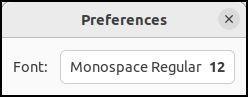
\includegraphics[width=4cm,height=1.6cm]{../image/pref_dialog.png}
\caption{Preference dialog}
\end{figure}

It has only one button, which is a GtkFontDialogButton widget. You can
add more widgets on the dialog but this simple dialog isn't so bad for
the first example program.

If the button is clicked, a FontDialog appears like this.

\begin{figure}
\centering
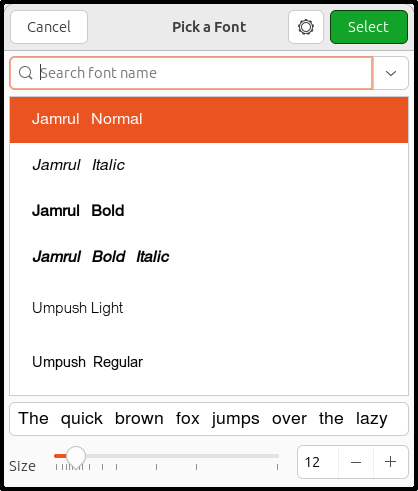
\includegraphics[width=6.27cm,height=7.38cm]{../image/fontdialog.png}
\caption{Font dialog}
\end{figure}

If the user chooses a font and clicks on the select button, the font is
changed.

GtkFontDialogButton and GtkFontDialog are available since GTK version
4.10. They replace GtkFontButton and GtkFontChooserDialog, which are
deprecated since 4.10.

\subsection{A composite widget}\label{a-composite-widget}

The preference dialog has GtkBox, GtkLabel and GtkFontButton in it and
is defined as a composite widget. The following is the template ui file
for TfePref.

\begin{lstlisting}[language=XML, numbers=left]
<?xml version="1.0" encoding="UTF-8"?>
<interface>
  <template class="TfePref" parent="GtkWindow">
    <property name="title">Preferences</property>
    <property name="resizable">FALSE</property>
    <property name="modal">TRUE</property>
    <child>
      <object class="GtkBox">
        <property name="orientation">GTK_ORIENTATION_HORIZONTAL</property>
        <property name="spacing">12</property>
        <property name="halign">GTK_ALIGN_CENTER</property>
        <property name="margin-start">12</property>
        <property name="margin-end">12</property>
        <property name="margin-top">12</property>
        <property name="margin-bottom">12</property>
        <child>
          <object class="GtkLabel">
            <property name="label">Font:</property>
            <property name="xalign">1</property>
          </object>
        </child>
        <child>
          <object class="GtkFontDialogButton" id="font_dialog_btn">
            <property name="dialog">
              <object class="GtkFontDialog"/>
            </property>
          </object>
        </child>
      </object>
    </child>
  </template>
</interface>
\end{lstlisting}

\begin{itemize}
\tightlist
\item
  Template tag specifies a composite widget. The class attribute
  specifies the class name, which is ``TfePref''. The parent attribute
  is \passthrough{\lstinline!GtkWindow!}. Therefore.
  \passthrough{\lstinline!TfePref!} is a child class of
  \passthrough{\lstinline!GtkWindow!}. A parent attribute is optional
  but it is recommended to write it explicitly. You can make TfePref as
  a child of \passthrough{\lstinline!GtkDialog!}, but
  \passthrough{\lstinline!GtkDialog!} is deprecated since version 4.10.
\item
  There are three properties, title, resizable and modal.
\item
  TfePref has a child widget GtkBox which is horizontal. The box has two
  children GtkLabel and GtkFontDialogButton.
\end{itemize}

\subsection{The header file}\label{the-header-file}

The file \passthrough{\lstinline!tfepref.h!} defines types and declares
a public function.

\begin{lstlisting}[language=C, numbers=left]
#pragma once

#include <gtk/gtk.h>

#define TFE_TYPE_PREF tfe_pref_get_type ()
G_DECLARE_FINAL_TYPE (TfePref, tfe_pref, TFE, PREF, GtkWindow)

GtkWidget *
tfe_pref_new (void);
\end{lstlisting}

\begin{itemize}
\tightlist
\item
  5: Defines the type \passthrough{\lstinline!TFE\_TYPE\_PREF!}, which
  is a macro replaced by
  \passthrough{\lstinline!tfe\_pref\_get\_type ()!}.
\item
  6: The macro \passthrough{\lstinline!G\_DECLAER\_FINAL\_TYPE!} expands
  to:

  \begin{itemize}
  \tightlist
  \item
    The function \passthrough{\lstinline!tfe\_pref\_get\_type ()!} is
    declared.
  \item
    TfePrep type is defined as a typedef of
    \passthrough{\lstinline!struct \_TfePrep!}.
  \item
    TfePrepClass type is defined as a typedef of
    \passthrough{\lstinline!struct \{GtkWindowClass *parent;\}!}.
  \item
    Two functions \passthrough{\lstinline!TFE\_PREF ()!} and
    \passthrough{\lstinline!TFE\_IS\_PREF ()!} is defined.
  \end{itemize}
\item
  8-9:The function \passthrough{\lstinline!tfe\_pref\_new!} is declared.
  It creates a new TfePref instance.
\end{itemize}

\subsection{The C file for composite
widget}\label{the-c-file-for-composite-widget}

The following codes are extracted from the file
\passthrough{\lstinline!tfepref.c!}.

\begin{lstlisting}[language=C]
#include <gtk/gtk.h>
#include "tfepref.h"

struct _TfePref
{
  GtkWindow parent;
  GtkFontDialogButton *font_dialog_btn;
};

G_DEFINE_FINAL_TYPE (TfePref, tfe_pref, GTK_TYPE_WINDOW);

static void
tfe_pref_dispose (GObject *gobject) {
  TfePref *pref = TFE_PREF (gobject);
  gtk_widget_dispose_template (GTK_WIDGET (pref), TFE_TYPE_PREF);
  G_OBJECT_CLASS (tfe_pref_parent_class)->dispose (gobject);
}

static void
tfe_pref_init (TfePref *pref) {
  gtk_widget_init_template (GTK_WIDGET (pref));
}

static void
tfe_pref_class_init (TfePrefClass *class) {
  G_OBJECT_CLASS (class)->dispose = tfe_pref_dispose;
  gtk_widget_class_set_template_from_resource (GTK_WIDGET_CLASS (class), "/com/github/ToshioCP/tfe/tfepref.ui");
  gtk_widget_class_bind_template_child (GTK_WIDGET_CLASS (class), TfePref, font_dialog_btn);
}

GtkWidget *
tfe_pref_new (void) {
  return GTK_WIDGET (g_object_new (TFE_TYPE_PREF, NULL));
}
\end{lstlisting}

\begin{itemize}
\tightlist
\item
  The structure \passthrough{\lstinline!\_TfePref!} has
  \passthrough{\lstinline!font\_dialog\_btn!} member. It points the
  GtkFontDialogButton object specified in the XML file ``tfepref.ui''.
  The member name \passthrough{\lstinline!font\_dialog\_btn!} must be
  the same as the GtkFontDialogButton id attribute in the XML file.
\item
  \passthrough{\lstinline!G\_DEFINE\_FINAL\_TYPE!} macro expands to:

  \begin{itemize}
  \tightlist
  \item
    The declaration of the functions
    \passthrough{\lstinline!tfe\_pref\_init!} and
    \passthrough{\lstinline!tfe\_pref\_class\_init!}. They are defined
    in the following part of the program.
  \item
    The definition of the variable
    \passthrough{\lstinline!tfe\_pref\_parent\_class!}.
  \item
    The definition of the function
    \passthrough{\lstinline!tfe\_pref\_get\_type!}.
  \end{itemize}
\item
  The function \passthrough{\lstinline!tfe\_pref\_class\_init!}
  initializes the TfePref class. The function
  \passthrough{\lstinline!gtk\_widget\_class\_set\_template\_from\_resource!}
  initializes the composite widget template from the XML resource. The
  function
  \passthrough{\lstinline!gtk\_widget\_class\_bind\_template\_child!}
  connects the TfePref structure member
  \passthrough{\lstinline!font\_dialog\_btn!} and the
  GtkFontDialogButton in the XML. The member name and the id attribute
  value must be the same.
\item
  The function \passthrough{\lstinline!tfe\_pref\_init!} initializes a
  newly created instance. The function
  \passthrough{\lstinline!gtk\_widget\_init\_template!} creates and
  initializes child widgets.
\item
  The function \passthrough{\lstinline!tfe\_pref\_dispose!} releases
  objects. The function
  \passthrough{\lstinline!gtk\_widget\_dispose\_template!} releases
  child widgets.
\end{itemize}

\subsection{GtkFontDialogButton and
Pango}\label{gtkfontdialogbutton-and-pango}

If the GtkFontDialogButton button is clicked, the GtkFontDialog dialog
appears. A user can choose a font on the dialog. If the user clicks on
the ``select'' button, the dialog disappears. And the font information
is given to the GtkFontDialogButton instance. The font data is taken
with the method
\passthrough{\lstinline!gtk\_font\_dialog\_button\_get\_font\_desc!}. It
returns a pointer to the PangoFontDescription structure.

Pango is a text layout engine. The
\href{https://docs.gtk.org/Pango/index.html}{documentation} is on the
internet.

PangoFontDescription is a C structure and it isn't allowed to access
directly. The document is
\href{https://docs.gtk.org/Pango/struct.FontDescription.html}{here}. If
you want to retrieve the font information, there are several functions.

\begin{itemize}
\tightlist
\item
  \passthrough{\lstinline!pango\_font\_description\_to\_string!} returns
  a string like ``Jamrul Bold Italic Semi-Expanded 12''.
\item
  \passthrough{\lstinline!pango\_font\_description\_get\_family!}
  returns a font family like ``Jamrul''.
\item
  \passthrough{\lstinline!pango\_font\_description\_get\_weight!}
  returns a PangoWeight constant like
  \passthrough{\lstinline!PANGO\_WEIGHT\_BOLD!}.
\item
  \passthrough{\lstinline!pango\_font\_description\_get\_style!} returns
  a PangoStyle constant like
  \passthrough{\lstinline!PANGO\_STYLE\_ITALIC!}.
\item
  \passthrough{\lstinline!pango\_font\_description\_get\_stretch!}
  returns a PangoStretch constant like
  \passthrough{\lstinline!PANGO\_STRETCH\_SEMI\_EXPANDED!}.
\item
  \passthrough{\lstinline!pango\_font\_description\_get\_size!} returns
  an integer like \passthrough{\lstinline!12!}. Its unit is point or
  pixel (device unit). The function
  \passthrough{\lstinline!pango\_font\_description\_get\_size\_is\_absolute!}
  returns TRUE if the unit is absolute that means device unit. Otherwise
  the unit is point.
\end{itemize}

\subsection{GSettings}\label{gsettings}

We want to maintain the font data after the application quits. There are
some ways to implement.

\begin{itemize}
\tightlist
\item
  Make a configuration file. For example, a text file
  ``\textasciitilde/.config/tfe/font\_desc.cfg'' keeps font information.
\item
  Use GSettings object. The basic idea of GSettings are similar to
  configuration file. Configuration information data is put into a
  database file.
\end{itemize}

GSettings is simple and easy to use but a bit hard to understand the
concept. This subsection describes the concept first and then how to
program it.

\subsubsection{GSettings schema}\label{gsettings-schema}

GSettings schema describes a set of keys, value types and some other
information. GSettings object uses this schema and it writes/reads the
value of a key to/from the right place in the database.

\begin{itemize}
\tightlist
\item
  A schema has an id. The id must be unique. We often use the same
  string as application id, but schema id and application id are
  different. You can use different name from application id. Schema id
  is a string delimited by periods. For example,
  ``com.github.ToshioCP.tfe'' is a correct schema id.
\item
  A schema usually has a path. The path is a location in the database.
  Each key is stored under the path. For example, if a key
  \passthrough{\lstinline!font-desc!} is defined with a path
  \passthrough{\lstinline!/com/github/ToshioCP/tfe/!}, the key's
  location in the database is
  \passthrough{\lstinline!/com/github/ToshioCP/tfe/font-desc!}. Path is
  a string begins with and ends with a slash
  (\passthrough{\lstinline!/!}). And it is delimited by slashes.
\item
  GSettings save information as key-value style. Key is a string begins
  with a lower case character followed by lower case, digit or dash
  (\passthrough{\lstinline!-!}) and ends with lower case or digit. No
  consecutive dashes are allowed. Values can be any type. GSettings
  stores values as GVariant type, which can be, for example, integer,
  double, boolean, string or complex types like an array. The type of
  values needs to be defined in the schema.
\item
  A default value needs to be set for each key.
\item
  A summery and description can be set for each key optionally.
\end{itemize}

Schemas are described in an XML format. For example,

\begin{lstlisting}[language=XML, numbers=left]
<?xml version="1.0" encoding="UTF-8"?>
<schemalist>
  <schema path="/com/github/ToshioCP/tfe/" id="com.github.ToshioCP.tfe">
    <key name="font-desc" type="s">
      <default>'Monospace 12'</default>
      <summary>Font</summary>
      <description>A font to be used for textview.</description>
    </key>
  </schema>
</schemalist>
\end{lstlisting}

\begin{itemize}
\tightlist
\item
  4: The type attribute is ``s''. It is GVariant type string. For
  GVariant type string, see
  \href{https://docs.gtk.org/glib/struct.VariantType.html\#gvariant-type-strings}{GLib
  API Reference -- GVariant Type Strings}. Other common types are:

  \begin{itemize}
  \tightlist
  \item
    ``b'': gboolean
  \item
    ``i'': gint32.
  \item
    ``d'': double.
  \end{itemize}
\end{itemize}

Further information is in:

\begin{itemize}
\tightlist
\item
  \href{https://docs.gtk.org/glib/gvariant-format-strings.html}{GLib API
  Reference -- GVariant Format Strings}
\item
  \href{https://docs.gtk.org/glib/gvariant-text.html}{GLib API Reference
  -- GVariant Text Format}
\item
  \href{https://docs.gtk.org/glib/struct.Variant.html}{GLib API
  Reference -- GVariant}
\item
  \href{https://docs.gtk.org/glib/struct.VariantType.html}{GLib API
  Reference -- VariantType}
\end{itemize}

\subsubsection{Gsettings command}\label{gsettings-command}

First, let's try \passthrough{\lstinline!gsettings!} application. It is
a configuration tool for GSettings.

\begin{lstlisting}
$ gsettings help
Usage:
  gsettings --version
  gsettings [--schemadir SCHEMADIR] COMMAND [ARGS?]

Commands:
  help                      Show this information
  list-schemas              List installed schemas
  list-relocatable-schemas  List relocatable schemas
  list-keys                 List keys in a schema
  list-children             List children of a schema
  list-recursively          List keys and values, recursively
  range                     Queries the range of a key
  describe                  Queries the description of a key
  get                       Get the value of a key
  set                       Set the value of a key
  reset                     Reset the value of a key
  reset-recursively         Reset all values in a given schema
  writable                  Check if a key is writable
  monitor                   Watch for changes

Use "gsettings help COMMAND" to get detailed help.
\end{lstlisting}

List schemas.

\begin{lstlisting}
$ gsettings list-schemas
org.gnome.rhythmbox.podcast
ca.desrt.dconf-editor.Demo.Empty
org.gnome.gedit.preferences.ui
org.gnome.evolution-data-server.calendar
org.gnome.rhythmbox.plugins.generic-player

... ...
\end{lstlisting}

Each line is an id of a schema. Each schema has a key-value
configuration data. You can see them with list-recursively command.
Let's look at the keys and values of
\passthrough{\lstinline!org.gnome.calculator!} schema.

\begin{lstlisting}
$ gsettings list-recursively org.gnome.calculator
org.gnome.calculator accuracy 9
org.gnome.calculator angle-units 'degrees'
org.gnome.calculator base 10
org.gnome.calculator button-mode 'basic'
org.gnome.calculator number-format 'automatic'
org.gnome.calculator precision 2000
org.gnome.calculator refresh-interval 604800
org.gnome.calculator show-thousands false
org.gnome.calculator show-zeroes false
org.gnome.calculator source-currency ''
org.gnome.calculator source-units 'degree'
org.gnome.calculator target-currency ''
org.gnome.calculator target-units 'radian'
org.gnome.calculator window-position (-1, -1)
org.gnome.calculator word-size 64
\end{lstlisting}

This schema is used by GNOME Calculator. Run the calculator and change
the mode, then check the schema again.

\begin{lstlisting}
$ gnome-calculator
\end{lstlisting}

\begin{figure}
\centering
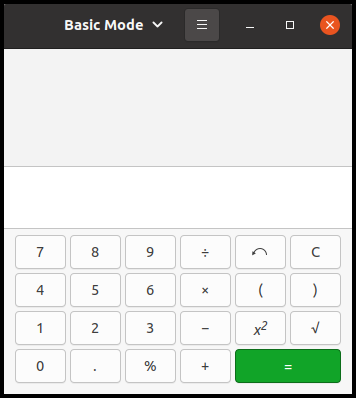
\includegraphics[width=5.34cm,height=5.97cm]{../image/gnome_calculator_basic.png}
\caption{gnome-calculator basic mode}
\end{figure}

Change the mode to advanced and quit.

\begin{figure}
\centering
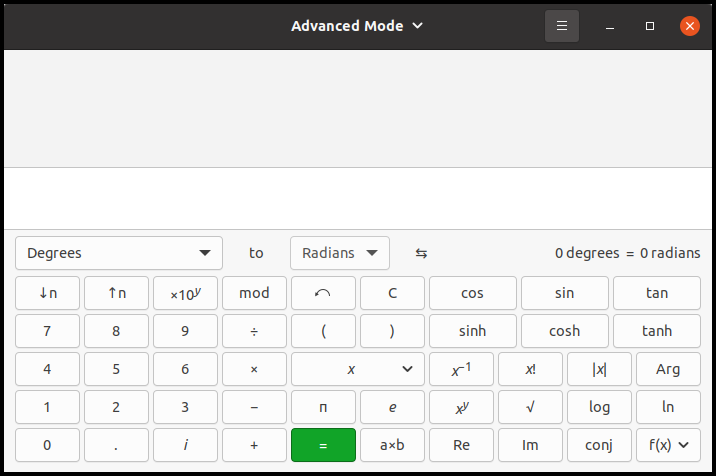
\includegraphics[width=10.74cm,height=7.14cm]{../image/gnome_calculator_advanced.png}
\caption{gnome-calculator advanced mode}
\end{figure}

Run gsettings and check the value of
\passthrough{\lstinline!button-mode!}.

\begin{lstlisting}
$ gsettings list-recursively org.gnome.calculator

... ...

org.gnome.calculator button-mode 'advanced'

... ...
\end{lstlisting}

Now we know that GNOME Calculator used gsettings and it has set
\passthrough{\lstinline!button-mode!} key to ``advanced''. The value
remains even the calculator quits. So when the calculator runs again, it
will appear as an advanced mode.

\subsubsection{Glib-compile-schemas
utility}\label{glib-compile-schemas-utility}

GSettings schemas are specified with an XML format. The XML schema files
must have the filename extension \passthrough{\lstinline!.gschema.xml!}.
The following is the XML schema file for the application
\passthrough{\lstinline!tfe!}.

\begin{lstlisting}[language=XML, numbers=left]
<?xml version="1.0" encoding="UTF-8"?>
<schemalist>
  <schema path="/com/github/ToshioCP/tfe/" id="com.github.ToshioCP.tfe">
    <key name="font-desc" type="s">
      <default>'Monospace 12'</default>
      <summary>Font</summary>
      <description>A font to be used for textview.</description>
    </key>
  </schema>
</schemalist>
\end{lstlisting}

The filename is ``com.github.ToshioCP.tfe.gschema.xml''. Schema XML
filenames are usually the schema id followed by ``.gschema.xml'' suffix.
You can use different name from schema id, but it is not recommended.

\begin{itemize}
\tightlist
\item
  2: The top level element is \passthrough{\lstinline!<schemalist>!}.
\item
  3: schema tag has \passthrough{\lstinline!path!} and
  \passthrough{\lstinline!id!} attributes. A path determines where the
  settings are stored in the conceptual global tree of settings. An id
  identifies the schema.
\item
  4: Key tag has two attributes. Name is the name of the key. Type is
  the type of the value of the key and it is a GVariant Format String.
\item
  5: default value of the key \passthrough{\lstinline!font-desc!} is
  \passthrough{\lstinline!Monospace 12!}.
\item
  6: Summery and description elements describes the key. They are
  optional, but it is recommended to add them in the XML file.
\end{itemize}

The XML file is compiled by glib-compile-schemas. When compiling,
\passthrough{\lstinline!glib-compile-schemas!} compiles all the XML
files which have ``.gschema.xml'' file extension in the directory given
as an argument. It converts the XML file into a binary file
\passthrough{\lstinline!gschemas.compiled!}. Suppose the XML file above
is under \passthrough{\lstinline!tfe6!} directory.

\begin{lstlisting}
$ glib-compile-schemas tfe6
\end{lstlisting}

Then, \passthrough{\lstinline!gschemas.compiled!} is generated under
\passthrough{\lstinline!tfe6!}. When you test your application, set
\passthrough{\lstinline!GSETTINGS\_SCHEMA\_DIR!} environment variable so
that GSettings objet can find
\passthrough{\lstinline!gschemas.compiled!}.

\begin{lstlisting}
$ GSETTINGS_SCHEMA_DIR=(the directory gschemas.compiled is located):$GSETTINGS_SCHEMA_DIR (your application name)
\end{lstlisting}

GSettings object looks for this file by the following process.

\begin{itemize}
\tightlist
\item
  It searches \passthrough{\lstinline!glib-2.0/schemas!} subdirectories
  of all the directories specified in the environment variable
  \passthrough{\lstinline!XDG\_DATA\_DIRS!}. Common directores are
  \passthrough{\lstinline!/usr/share/glib-2.0/schemas!} and
  \passthrough{\lstinline!/usr/local/share/glib-2.0/schemas!}.
\item
  If \passthrough{\lstinline!$HOME/.local/share/glib-2.0/schemas!}
  exists, it is also searched.
\item
  If \passthrough{\lstinline!GSETTINGS\_SCHEMA\_DIR!} environment
  variable is defined, it searches all the directories specified in the
  variable. \passthrough{\lstinline!GSETTINGS\_SCHEMA\_DIR!} can specify
  multiple directories delimited by colon (:).
\end{itemize}

The directories above includes more than one
\passthrough{\lstinline!.gschema.xml!} file. Therefore, when you install
your application, follow the instruction below to install your schemas.

\begin{enumerate}
\def\labelenumi{\arabic{enumi}.}
\tightlist
\item
  Make \passthrough{\lstinline!.gschema.xml!} file.
\item
  Copy it to one of the directories above. For example,
  \passthrough{\lstinline!$HOME/.local/share/glib-2.0/schemas!}.
\item
  Run \passthrough{\lstinline!glib-compile-schemas!} on the directory.
  It compiles all the schema files in the directory and creates or
  updates the database file \passthrough{\lstinline!gschemas.compiled!}.
\end{enumerate}

\subsubsection{GSettings object and
binding}\label{gsettings-object-and-binding}

Now, we go on to the next topic, how to program GSettings.

You need to compile your schema file in advance.

Suppose id, key, class name and a property name are:

\begin{itemize}
\tightlist
\item
  GSettings id: com.github.ToshioCP.sample
\item
  GSettings key: sample\_key
\item
  The class name: Sample
\item
  The property to bind: sample\_property
\end{itemize}

The example below uses \passthrough{\lstinline!g\_settings\_bind!}. If
you use it, GSettings key and instance property must have the same the
type. In the example, it is assumed that the type of ``sample\_key'' and
``sample\_property'' are the same.

\begin{lstlisting}[language=C]
GSettings *settings;
Sample *sample_object;

settings = g_settings_new ("com.github.ToshioCP.sample");
sample_object = sample_new ();
g_settings_bind (settings, "sample_key", sample_object, "sample_property", G_SETTINGS_BIND_DEFAULT);
\end{lstlisting}

The function \passthrough{\lstinline!g\_settings\_bind!} binds the
GSettings value and the property of the instance. If the property value
is changed, the GSettings value is also changed, and vice versa. The two
values are always the same.

The function \passthrough{\lstinline!g\_settings\_bind!} is simple and
easy but it isn't always possible. The type of GSettings are restricted
to the type GVariant has. Some property types are out of GVariant. For
example, GtkFontDialogButton has ``font-desc'' property and its type is
PangoFontDescription. PangoFontDescription is a C structure and it is
wrapped in a boxed type GValue to store in the property. GVariant
doesn't support boxed type.

In that case, another function
\passthrough{\lstinline!g\_settings\_bind\_with\_mapping!} is used. It
binds GSettings GVariant value and object property via GValue with
mapping functions.

\begin{lstlisting}[language=C]
void
g_settings_bind_with_mapping (
  GSettings* settings,
  const gchar* key,
  GObject* object,
  const gchar* property,
  GSettingsBindFlags flags, // G_SETTINGS_BIND_DEFAULT is commonly used
  GSettingsBindGetMapping get_mapping, // GSettings => property, See the example below
  GSettingsBindSetMapping set_mapping, // property => GSettings, See the example below
  gpointer user_data, // NULL if unnecessary
  GDestroyNotify destroy //NULL if unnecessary
)
\end{lstlisting}

The mapping functions are defined like these:

\begin{lstlisting}[language=C]
gboolean
(* GSettingsBindGetMapping) (
  GValue* value,
  GVariant* variant,
  gpointer user_data
)

GVariant*
(* GSettingsBindSetMapping) (
  const GValue* value,
  const GVariantType* expected_type,
  gpointer user_data
)
\end{lstlisting}

The following codes are extracted from
\passthrough{\lstinline!tfepref.c!}.

\begin{lstlisting}[language=C, numbers=left]
static gboolean // GSettings => property
get_mapping (GValue* value, GVariant* variant, gpointer user_data) {
  const char *s = g_variant_get_string (variant, NULL);
  PangoFontDescription *font_desc = pango_font_description_from_string (s);
  g_value_take_boxed (value, font_desc);
  return TRUE;
}

static GVariant* // Property => GSettings
set_mapping (const GValue* value, const GVariantType* expected_type, gpointer user_data) {
  char*font_desc_string = pango_font_description_to_string (g_value_get_boxed (value));
  return g_variant_new_take_string (font_desc_string);
}

static void
tfe_pref_init (TfePref *pref) {
  gtk_widget_init_template (GTK_WIDGET (pref));
  pref->settings = g_settings_new ("com.github.ToshioCP.tfe");
  g_settings_bind_with_mapping (pref->settings, "font-desc", pref->font_dialog_btn, "font-desc", G_SETTINGS_BIND_DEFAULT,
      get_mapping, set_mapping, NULL, NULL);
}
\end{lstlisting}

\begin{itemize}
\tightlist
\item
  15-21: This function \passthrough{\lstinline!tfe\_pref\_init!}
  initializes the new TfePref instance.
\item
  18: Creates a new GSettings instance. The id is
  ``com.github.ToshioCP.tfe''.
\item
  19-20: Binds the GSettings ``font-desc'' and the GtkFontDialogButton
  property ``font-desc''. The mapping functions are
  \passthrough{\lstinline!get\_mapping!} and
  \passthrough{\lstinline!set\_mapping!}.
\item
  1-7: The mapping function from GSettings to the property. The first
  argument \passthrough{\lstinline!value!} is a GValue to be stored in
  the property. The second argument \passthrough{\lstinline!variant!} is
  a GVarinat structure that comes from the GSettings value.
\item
  3: Retrieves a string from the GVariant structure.
\item
  4: Build a PangoFontDescription structure from the string and assigns
  its address to \passthrough{\lstinline!font\_desc!}.
\item
  5: Puts \passthrough{\lstinline!font\_desc!} into the GValue
  \passthrough{\lstinline!value!}. The ownership of
  \passthrough{\lstinline!font\_desc!} moves to
  \passthrough{\lstinline!value!}.
\item
  6: Returns TRUE that means the mapping succeeds.
\item
  9-13: The mapping function from the property to GSettings. The first
  argument \passthrough{\lstinline!value!} holds the property data. The
  second argument \passthrough{\lstinline!expected\_type!} is the type
  of GVariant that the GSettings value has. It isn't used in this
  function.
\item
  11: Gets the PangoFontDescription structure from
  \passthrough{\lstinline!value!} and converts it to string.
\item
  12: The string is inserted to a GVariant structure. The ownership of
  the string \passthrough{\lstinline!font\_desc\_string!} moves to the
  returned value.
\end{itemize}

\subsection{C file}\label{c-file}

The following is the full codes of \passthrough{\lstinline!tfepref.c!}

\begin{lstlisting}[language=C, numbers=left]
#include <gtk/gtk.h>
#include "tfepref.h"

struct _TfePref
{
  GtkWindow parent;
  GSettings *settings;
  GtkFontDialogButton *font_dialog_btn;
};

G_DEFINE_FINAL_TYPE (TfePref, tfe_pref, GTK_TYPE_WINDOW);

static void
tfe_pref_dispose (GObject *gobject) {
  TfePref *pref = TFE_PREF (gobject);

  /* GSetting bindings are automatically removed when the object is finalized, so it isn't necessary to unbind them explicitly.*/
  g_clear_object (&pref->settings);
  gtk_widget_dispose_template (GTK_WIDGET (pref), TFE_TYPE_PREF);
  G_OBJECT_CLASS (tfe_pref_parent_class)->dispose (gobject);
}

/* ---------- get_mapping/set_mapping ---------- */
static gboolean // GSettings => property
get_mapping (GValue* value, GVariant* variant, gpointer user_data) {
  const char *s = g_variant_get_string (variant, NULL);
  PangoFontDescription *font_desc = pango_font_description_from_string (s);
  g_value_take_boxed (value, font_desc);
  return TRUE;
}

static GVariant* // Property => GSettings
set_mapping (const GValue* value, const GVariantType* expected_type, gpointer user_data) {
  char*font_desc_string = pango_font_description_to_string (g_value_get_boxed (value));
  return g_variant_new_take_string (font_desc_string);
}

static void
tfe_pref_init (TfePref *pref) {
  gtk_widget_init_template (GTK_WIDGET (pref));
  pref->settings = g_settings_new ("com.github.ToshioCP.tfe");
  g_settings_bind_with_mapping (pref->settings, "font-desc", pref->font_dialog_btn, "font-desc", G_SETTINGS_BIND_DEFAULT,
      get_mapping, set_mapping, NULL, NULL);
}

static void
tfe_pref_class_init (TfePrefClass *class) {
  G_OBJECT_CLASS (class)->dispose = tfe_pref_dispose;
  gtk_widget_class_set_template_from_resource (GTK_WIDGET_CLASS (class), "/com/github/ToshioCP/tfe/tfepref.ui");
  gtk_widget_class_bind_template_child (GTK_WIDGET_CLASS (class), TfePref, font_dialog_btn);
}

GtkWidget *
tfe_pref_new (void) {
  return GTK_WIDGET (g_object_new (TFE_TYPE_PREF, NULL));
}
\end{lstlisting}

\subsection{Test program}\label{test-program}

There's a test program located at
\passthrough{\lstinline!src/tfe6/test!} directory.

\begin{lstlisting}[language=C, numbers=left]
#include <gtk/gtk.h>
#include "../tfepref.h"

GSettings *settings;

// "changed::font-desc" signal handler
static void
changed_font_desc_cb (GSettings *settings, char *key, gpointer user_data) {
  char *s;
  s = g_settings_get_string (settings, key);
  g_print ("%s\n", s);
  g_free (s);
}

static void
app_shutdown (GApplication *application) {
  g_object_unref (settings);
}

static void
app_activate (GApplication *application) {
  GtkWidget *pref = tfe_pref_new ();

  gtk_window_set_application (GTK_WINDOW (pref), GTK_APPLICATION (application));
  gtk_window_present (GTK_WINDOW (pref));
}

static void
app_startup (GApplication *application) {
  settings = g_settings_new ("com.github.ToshioCP.tfe");
  g_signal_connect (settings, "changed::font-desc", G_CALLBACK (changed_font_desc_cb), NULL);
  g_print ("%s\n", "Change the font with the font button. Then the new font will be printed out.\n");
}

#define APPLICATION_ID "com.github.ToshioCP.test_tfe_pref"

int
main (int argc, char **argv) {
  GtkApplication *app;
  int stat;

  app = gtk_application_new (APPLICATION_ID, G_APPLICATION_DEFAULT_FLAGS);
  g_signal_connect (app, "startup", G_CALLBACK (app_startup), NULL);
  g_signal_connect (app, "activate", G_CALLBACK (app_activate), NULL);
  g_signal_connect (app, "shutdown", G_CALLBACK (app_shutdown), NULL);
  stat =g_application_run (G_APPLICATION (app), argc, argv);
  g_object_unref (app);
  return stat;
}
\end{lstlisting}

This program sets its active window to TfePref instance, which is a
child object of GtkWindow.

It sets the ``changed::font-desc'' signal handler in the startup
function. The process from the user's font selection to the handler is:

\begin{itemize}
\tightlist
\item
  The user clicked on the GtkFontDialogButton and GtkFontDialog appears.
\item
  He/she selects a new font.
\item
  The ``font-desc'' property of the GtkFontDialogButton instance is
  changed.
\item
  The value of ``font-desc'' key on the GSettings database is changed
  since it is bound to the property.
\item
  The ``changed::font-desc'' signal on the GSettings instance is
  emitted.
\item
  The handler is called.
\end{itemize}

The program building is divided into four steps.

\begin{itemize}
\tightlist
\item
  Compile the schema file
\item
  Compile the XML file to a resource (C source file)
\item
  Compile the C files
\item
  Run the executable file
\end{itemize}

Commands are shown in the next four sub-subsections. You don't need to
try them. The final sub-subsection shows the meson-ninja way, which is
the easiest.

\subsubsection{Compile the schema file}\label{compile-the-schema-file}

\begin{lstlisting}
$ cd src/tef6/test
$ cp ../com.github.ToshioCP.tfe.gschema.xml com.github.ToshioCP.tfe.gschema.xml
$ glib-compile-schemas .
\end{lstlisting}

Be careful. The commands \passthrough{\lstinline!glib-compile-schemas!}
has an argument ``.'', which means the current directory. This results
in creating \passthrough{\lstinline!gschemas.compiled!} file.

\subsubsection{Compile the XML file}\label{compile-the-xml-file}

\begin{lstlisting}
$ glib-compile-resources --sourcedir=.. --generate-source --target=resource.c ../tfe.gresource.xml
\end{lstlisting}

\subsubsection{Compile the C file}\label{compile-the-c-file}

\begin{lstlisting}
$ gcc `pkg-config --cflags gtk4` test_pref.c ../tfepref.c resource.c `pkg-config --libs gtk4`
\end{lstlisting}

\subsubsection{Run the executable file}\label{run-the-executable-file}

\begin{lstlisting}
$ GSETTINGS_SCHEMA_DIR=. ./a.out

Jamrul Italic Semi-Expanded 12 # <= select Jamrul Italic 12
Monospace 12 #<= select Monospace Regular 12
\end{lstlisting}

\subsubsection{Meson-ninja way}\label{meson-ninja-way}

Meson wraps up the commands above. Create the following text and save it
to \passthrough{\lstinline!meson.build!}.

Note: Gtk4-tutorial repository has meson.build file that defines several
tests. So you can try it instead of the following text.

\begin{lstlisting}
project('tfe_pref_test', 'c')

gtkdep = dependency('gtk4')

gnome=import('gnome')
resources = gnome.compile_resources('resources','../tfe.gresource.xml', source_dir: '..')
gnome.compile_schemas(build_by_default: true, depend_files: 'com.github.ToshioCP.tfe.gschema.xml')

executable('test_pref', ['test_pref.c', '../tfepref.c'], resources, dependencies: gtkdep, export_dynamic: true, install: false)
\end{lstlisting}

\begin{itemize}
\tightlist
\item
  Project name is `tfe\_pref\_test' and it is written in C language.
\item
  It depends on GTK4 library.
\item
  It uses GNOME module. Modules are prepared by Meson.
\item
  GNOME module has \passthrough{\lstinline!compile\_resources!} method.
  When you call this method, you need the prefix ``gnome.''.

  \begin{itemize}
  \tightlist
  \item
    The target filename is resources.
  \item
    The definition XML file is `../tfe.gresource.xml'.
  \item
    The source dir is `..'. All the ui files are located there.
  \end{itemize}
\item
  GNOME module has \passthrough{\lstinline!compile\_schemas!} method. It
  compiles the schema file `com.github.ToshioCP.tfe.gschema.xml'. You
  need to copy `../com.github.ToshioCP.tfe.gschema.xml' to the current
  directory in advance.
\item
  It creates an executable file `test\_pref'. The source files are
  `test\_pref.c', `../tfepref.c' and
  \passthrough{\lstinline!resources!}, which is made by
  \passthrough{\lstinline!gnome.compile\_resources!}. It depends on
  \passthrough{\lstinline!gtkdep!}, which is GTK4 library. The symbols
  are exported and no installation support.
\end{itemize}

Type like this to build and test the program.

\begin{lstlisting}
$ cd src/tef6/test
$ cp ../com.github.ToshioCP.tfe.gschema.xml com.github.ToshioCP.tfe.gschema.xml
$ meson setup _build
$ ninja -C _build
$ GSETTINGS_SCHEMA_DIR=_build _build/test_pref
\end{lstlisting}

A window appears and you can choose a font via GtkFontDialog. If you
select a new font, the font string is output through the standard
output.

  \section{TfeWindow}\label{tfewindow}

\subsection{The Tfe window and XML
files}\label{the-tfe-window-and-xml-files}

The following is the window of Tfe.

\begin{figure}
\centering
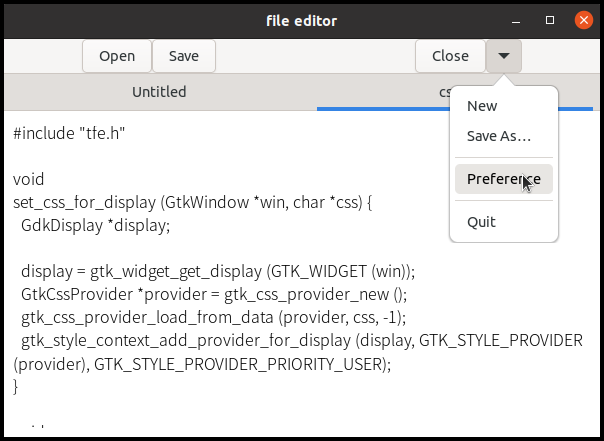
\includegraphics[width=9.06cm,height=6.615cm]{../image/tfe6.png}
\caption{tfe6}
\end{figure}

\begin{itemize}
\tightlist
\item
  Open, save and close buttons are placed on the toolbar. In addition,
  GtkMenuButton is added to the toolbar. This button shows a popup menu
  when clicked on. Here, popup means widely, including pull-down menu.
\item
  New, save-as, preference and quit items are put into the menu.
\end{itemize}

This makes the most frequently used operation bound to the tool bar
buttons. And the others are stored in behind the menus. So, it is more
practical.

The window is a composite widget. The definition is described in the XML
file \passthrough{\lstinline!tfewindow.ui!}.

\begin{lstlisting}[language=XML, numbers=left]
<?xml version="1.0" encoding="UTF-8"?>
<interface>
  <template class="TfeWindow" parent="GtkApplicationWindow">
    <property name="title">Text File Editor</property>
    <property name="default-width">600</property>
    <property name="default-height">400</property>
    <child>
      <object class="GtkBox" id="boxv">
        <property name="orientation">GTK_ORIENTATION_VERTICAL</property>
        <child>
          <object class="GtkBox" id="boxh">
            <property name="orientation">GTK_ORIENTATION_HORIZONTAL</property>
            <child>
              <object class="GtkLabel">
                <property name="width-chars">10</property>
              </object>
            </child>
            <child>
              <object class="GtkButton">
                <property name="label">Open</property>
                <property name="action-name">win.open</property>
              </object>
            </child>
            <child>
              <object class="GtkButton">
                <property name="label">Save</property>
                <property name="action-name">win.save</property>
              </object>
            </child>
            <child>
              <object class="GtkLabel">
                <property name="hexpand">TRUE</property>
              </object>
            </child>
            <child>
              <object class="GtkButton">
                <property name="label">Close</property>
                <property name="action-name">win.close</property>
              </object>
            </child>
            <child>
              <object class="GtkMenuButton" id="btnm">
                <property name="direction">down</property>
                <property name="icon-name">open-menu-symbolic</property>
              </object>
            </child>
            <child>
              <object class="GtkLabel">
                <property name="width-chars">10</property>
              </object>
            </child>
          </object>
        </child>
        <child>
          <object class="GtkNotebook" id="nb">
            <property name="scrollable">TRUE</property>
            <property name="hexpand">TRUE</property>
            <property name="vexpand">TRUE</property>
          </object>
        </child>
      </object>
    </child>
  </template>
</interface>
\end{lstlisting}

\begin{itemize}
\tightlist
\item
  Three buttons ``Open'', ``Save'' and ``Close'' are defined. You can
  use two ways to catch the button click event. The one is ``clicked''
  signal and the other is to register an action to the button. The first
  way is simple. You can connects the signal and your handler directly.
  The second way is like menu items. When the button is clicked, the
  corresponding action is activated. It is a bit complicated because you
  need to create an action and its ``activate'' handler in advance. But
  one advantage is you can connect two or more things to the action. For
  example, an accelerator can be connected to the action. Accelerators
  are keys that connects to actions. For example, Ctrl+O is often
  connected to a file open action. So, both open button and Ctrl+O
  activates an open action. The latter way is used in the XML file
  above.
\item
  You can specify a theme icon to GtkMenuButton with ``icon-name''
  poperty. The ``open-menu-symbolic'' is an image that is called
  hamburger menu.
\end{itemize}

The \passthrough{\lstinline!menu.ui!} XML file defines the menu for
GtkMenuButton.

\begin{lstlisting}[language=XML, numbers=left]
<?xml version="1.0" encoding="UTF-8"?>
<interface>
  <menu id="menu">
    <section>
      <item>
        <attribute name="label">New</attribute>
        <attribute name="action">win.new</attribute>
      </item>
      <item>
        <attribute name="label">Save As…</attribute>
        <attribute name="action">win.saveas</attribute>
      </item>
    </section>
    <section>
      <item>
        <attribute name="label">Preference</attribute>
        <attribute name="action">win.pref</attribute>
      </item>
    </section>
    <section>
      <item>
        <attribute name="label">Quit</attribute>
        <attribute name="action">win.close-all</attribute>
      </item>
    </section>
  </menu>
</interface>
\end{lstlisting}

There are four menu items and they are connected to actions.

\subsection{The header file}\label{the-header-file}

The following is the codes of \passthrough{\lstinline!tfewindow.h!}.

\begin{lstlisting}[language=C, numbers=left]
#pragma once

#include <gtk/gtk.h>

#define TFE_TYPE_WINDOW tfe_window_get_type ()
G_DECLARE_FINAL_TYPE (TfeWindow, tfe_window, TFE, WINDOW, GtkApplicationWindow)

void
tfe_window_notebook_page_new (TfeWindow *win);

void
tfe_window_notebook_page_new_with_files (TfeWindow *win, GFile **files, int n_files);

GtkWidget *
tfe_window_new (GtkApplication *app);
\end{lstlisting}

\begin{itemize}
\tightlist
\item
  5-6: \passthrough{\lstinline!TFE\_TYPE\_WINDOW!} definition and the
  \passthrough{\lstinline!G\_DECLARE\_FINAL\_TYPE!} macro.
\item
  8-15: Public functions. The first two functions creates a notebook
  page and the last function creates a window.
\end{itemize}

\subsection{C file}\label{c-file}

\subsubsection{A composite widget}\label{a-composite-widget}

The following codes are extracted from
\passthrough{\lstinline!tfewindow.c!}.

\begin{lstlisting}[language=C]
#include <gtk/gtk.h>
#include "tfewindow.h"

struct _TfeWindow {
  GtkApplicationWindow parent;
  GtkMenuButton *btnm;
  GtkNotebook *nb;
  gboolean is_quit;
};

G_DEFINE_FINAL_TYPE (TfeWindow, tfe_window, GTK_TYPE_APPLICATION_WINDOW);

static void
tfe_window_dispose (GObject *gobject) {
  gtk_widget_dispose_template (GTK_WIDGET (gobject), TFE_TYPE_WINDOW);
  G_OBJECT_CLASS (tfe_window_parent_class)->dispose (gobject);
}

static void
tfe_window_init (TfeWindow *win) {
  GtkBuilder *build;
  GMenuModel *menu;

  gtk_widget_init_template (GTK_WIDGET (win));

  build = gtk_builder_new_from_resource ("/com/github/ToshioCP/tfe/menu.ui");
  menu = G_MENU_MODEL (gtk_builder_get_object (build, "menu"));
  gtk_menu_button_set_menu_model (win->btnm, menu);
  g_object_unref(build);
... ... ...
}

static void
tfe_window_class_init (TfeWindowClass *class) {
  GObjectClass *object_class = G_OBJECT_CLASS (class);

  object_class->dispose = tfe_window_dispose;
  gtk_widget_class_set_template_from_resource (GTK_WIDGET_CLASS (class), "/com/github/ToshioCP/tfe/tfewindow.ui");
  gtk_widget_class_bind_template_child (GTK_WIDGET_CLASS (class), TfeWindow, btnm);
  gtk_widget_class_bind_template_child (GTK_WIDGET_CLASS (class), TfeWindow, nb);
}

GtkWidget *
tfe_window_new (GtkApplication *app) {
  return GTK_WIDGET (g_object_new (TFE_TYPE_WINDOW, "application", app, NULL));
}
\end{lstlisting}

The program above is similar to \passthrough{\lstinline!tfealert.c!} and
\passthrough{\lstinline!tfepref.c!}. It uses the same way to build a
composite widget. But there's one thing new. It is menu. The menu is
built from the XML resource \passthrough{\lstinline!menu.ui!} and
inserted into the menu button. It is done in the instance initialization
function \passthrough{\lstinline!tfe\_window\_init!}.

\subsubsection{Actions}\label{actions}

Actions can belong to an application or window. Tfe only has one top
window and all the actions are registered in the window. For example,
``close-all'' action destroys the top level window and that brings the
application to quit. You can make ``app.quit'' action instead of
``win.close-all''. It's your choice. If your application has two or more
windows, both ``app.quit'' and ``win:close-all'', which closes all the
notebook pages on the window, may be necessary. Anyway, you need to
consider that each action should belong to the application or a window.

Actions are defined in the instance initialization function.

\begin{lstlisting}[language=C]
static void
tfe_window_init (TfeWindow *win) {
... ... ...
/* ----- action ----- */
  const GActionEntry win_entries[] = {
    { "open", open_activated, NULL, NULL, NULL },
    { "save", save_activated, NULL, NULL, NULL },
    { "close", close_activated, NULL, NULL, NULL },
    { "new", new_activated, NULL, NULL, NULL },
    { "saveas", saveas_activated, NULL, NULL, NULL },
    { "pref", pref_activated, NULL, NULL, NULL },
    { "close-all", close_all_activated, NULL, NULL, NULL }
  };
  g_action_map_add_action_entries (G_ACTION_MAP (win), win_entries, G_N_ELEMENTS (win_entries), win);
... ... ...
}
\end{lstlisting}

Two things are necessary, an array and the
\passthrough{\lstinline!g\_action\_map\_add\_action\_entries!} function.

\begin{itemize}
\tightlist
\item
  The element of the array is the GActionEntry structure. The structure
  has the following members:

  \begin{itemize}
  \tightlist
  \item
    an action name
  \item
    a handler for the activate signal
  \item
    the type of the parameter or NULL for no parameter
  \item
    the initial state for the action
  \item
    a handler for the change-state signal
  \end{itemize}
\item
  The actions above are stateless and have no parameters. So, the third
  parameter and after are all NULL.
\item
  The function
  \passthrough{\lstinline!g\_action\_map\_add\_action\_entries!} adds
  the actions in the \passthrough{\lstinline!win\_entries!} array to the
  action map \passthrough{\lstinline!win!}. The last argument
  \passthrough{\lstinline!win!} is the user\_data, which is the last
  argument of handlers.
\item
  All the handlers are in \passthrough{\lstinline!tfewindow.c!} program
  and shown in the following subsections.
\end{itemize}

\subsubsection{The handlers of the
actions}\label{the-handlers-of-the-actions}

\paragraph{open\_activated}\label{open_activated}

The callback function \passthrough{\lstinline!open\_activated!} is an
activate signal handler on ``open'' action.

\begin{lstlisting}[language=C, numbers=left]
static void
open_activated (GSimpleAction *action, GVariant *parameter, gpointer user_data) {
  TfeWindow *win = TFE_WINDOW (user_data);
  GtkWidget *tv = tfe_text_view_new ();

  g_signal_connect (TFE_TEXT_VIEW (tv), "open-response", G_CALLBACK (open_response_cb), win);
  tfe_text_view_open (TFE_TEXT_VIEW (tv), GTK_WINDOW (win));
}
\end{lstlisting}

It connects the ``open-response'' signal on the newly created
TfeTextView instance and just calls
\passthrough{\lstinline!tfe\_text\_view\_open!}. It leaves the rest of
the task to the signal handler
\passthrough{\lstinline!open\_response\_cb!}.

\begin{lstlisting}[language=C, numbers=left]
static void
open_response_cb (TfeTextView *tv, int response, gpointer user_data) {
  TfeWindow *win = TFE_WINDOW (user_data);
  GFile *file;
  char *filename;

  if (response != TFE_OPEN_RESPONSE_SUCCESS) {
    g_object_ref_sink (tv);
    g_object_unref (tv);
  }else if (! G_IS_FILE (file = tfe_text_view_get_file (tv))) {
    g_object_ref_sink (tv);
    g_object_unref (tv);
  }else {
    filename = g_file_get_basename (file);
    g_object_unref (file);
    notebook_page_build (win, GTK_WIDGET (tv), filename);
    g_free (filename);
  }
}
\end{lstlisting}

If the TfeTextView instance failed to read a file, it destroys the
instance with \passthrough{\lstinline!g\_object\_ref\_sink!} and
\passthrough{\lstinline!g\_object\_unref!}. Since newly created widgets
are floating, you need to convert the floating reference to the normal
reference before you release it. The conversion is done with
\passthrough{\lstinline!g\_object\_ref\_sink!}.

If the instance successfully read the file, it calls
\passthrough{\lstinline!notebook\_page\_build!} to build a notebook page
and add it to the GtkNotebook object.

\begin{lstlisting}[language=C, numbers=left]
static void
notebook_page_build (TfeWindow *win, GtkWidget *tv, char *filename) {
  // The arguments win, tb and filename are owned by the caller.
  // If tv has a floating reference, it is consumed by the function.
  GtkWidget *scr = gtk_scrolled_window_new ();
  GtkTextBuffer *tb = gtk_text_view_get_buffer (GTK_TEXT_VIEW (tv));
  GtkNotebookPage *nbp;
  GtkWidget *lab;
  int i;

  gtk_text_view_set_wrap_mode (GTK_TEXT_VIEW (tv), GTK_WRAP_WORD_CHAR);
  gtk_scrolled_window_set_child (GTK_SCROLLED_WINDOW (scr), tv);
  lab = gtk_label_new (filename);
  i = gtk_notebook_append_page (win->nb, scr, lab);
  nbp = gtk_notebook_get_page (win->nb, scr);
  g_object_set (nbp, "tab-expand", TRUE, NULL);
  gtk_notebook_set_current_page (win->nb, i);
  g_signal_connect (GTK_TEXT_VIEW (tv), "change-file", G_CALLBACK (file_changed_cb), win->nb);
  g_signal_connect (tb, "modified-changed", G_CALLBACK (modified_changed_cb), tv);
}
\end{lstlisting}

This function is a kind of library function and it is called from the
different three places.

This function creates a new GtkScrolledWindow instance and sets its
child to \passthrough{\lstinline!tv!}. Then it appends it to the
GtkNotebook instance \passthrough{\lstinline!win->nb!}. And it sets the
tab label to the filename.

After the building, it connects two signals and handlers.

\begin{itemize}
\tightlist
\item
  ``change-file'' signal and \passthrough{\lstinline!file\_changed\_cb!}
  handler. If the TfeTextView instance changes the file, the handler is
  called and the notebook page tab is updated.
\item
  ``modified-changed'' signal and
  \passthrough{\lstinline!modified\_changed\_cb!} handler. If the text
  in the buffer of TfeTextView instance is modified, an asterisk is
  added at the beginning of the filename of the notebook page tab. If
  the text is saved to the file, the asterisk is removed. The asterisk
  tells the user that the text has been modified or not.
\end{itemize}

\begin{lstlisting}[language=C, numbers=left]
static void
file_changed_cb (TfeTextView *tv, gpointer user_data) {
  GtkNotebook *nb =  GTK_NOTEBOOK (user_data);
  GtkWidget *scr;
  GtkWidget *label;
  GFile *file;
  char *filename;

  file = tfe_text_view_get_file (tv);
  scr = gtk_widget_get_parent (GTK_WIDGET (tv));
  if (G_IS_FILE (file)) {
    filename = g_file_get_basename (file);
    g_object_unref (file);
  } else
    filename = get_untitled ();
  label = gtk_label_new (filename);
  g_free (filename);
  gtk_notebook_set_tab_label (GTK_NOTEBOOK (nb), scr, label);
}

static void
modified_changed_cb (GtkTextBuffer *tb, gpointer user_data) {
  TfeTextView *tv = TFE_TEXT_VIEW (user_data);
  GtkWidget *scr = gtk_widget_get_parent (GTK_WIDGET (tv));
  GtkWidget *nb =  gtk_widget_get_ancestor (GTK_WIDGET (tv), GTK_TYPE_NOTEBOOK);
  GtkWidget *label;
  GFile *file;
  char *filename;
  char *text;

  file = tfe_text_view_get_file (tv);
  filename = g_file_get_basename (file);
  if (gtk_text_buffer_get_modified (tb))
    text = g_strdup_printf ("*%s", filename);
  else
    text = g_strdup (filename);
  g_object_unref (file);
  g_free (filename);
  label = gtk_label_new (text);
  g_free (text);
  gtk_notebook_set_tab_label (GTK_NOTEBOOK (nb), scr, label);
}
\end{lstlisting}

\paragraph{save\_activated}\label{save_activated}

The callback function \passthrough{\lstinline!save\_activated!} is an
activate signal handler on ``save'' action.

\begin{lstlisting}[language=C, numbers=left]
static void
save_activated (GSimpleAction *action, GVariant *parameter, gpointer user_data) {
  TfeWindow *win = TFE_WINDOW (user_data);
  TfeTextView *tv = get_current_textview (win->nb);

  tfe_text_view_save (TFE_TEXT_VIEW (tv));
}
\end{lstlisting}

This function gets the current TfeTextView instance with the function
\passthrough{\lstinline!get\_current\_textview!}. And it just calls
\passthrough{\lstinline!tfe\_text\_view\_save!}.

\begin{lstlisting}[language=C, numbers=left]
static TfeTextView *
get_current_textview (GtkNotebook *nb) {
  int i;
  GtkWidget *scr;
  GtkWidget *tv;

  i = gtk_notebook_get_current_page (nb);
  scr = gtk_notebook_get_nth_page (nb, i);
  tv = gtk_scrolled_window_get_child (GTK_SCROLLED_WINDOW (scr));
  return TFE_TEXT_VIEW (tv);
}
\end{lstlisting}

\paragraph{close\_activated}\label{close_activated}

The callback function \passthrough{\lstinline!close\_activated!} is an
activate signal handler on ``close'' action. It closes the current
notebook page.

\begin{lstlisting}[language=C, numbers=left]
static void
close_activated (GSimpleAction *action, GVariant *parameter, gpointer user_data) {
  TfeWindow *win = TFE_WINDOW (user_data);
  TfeTextView *tv;
  GtkTextBuffer *tb;
  GtkWidget *alert;

  tv = get_current_textview (win->nb);
  tb = gtk_text_view_get_buffer (GTK_TEXT_VIEW (tv));
  if (! gtk_text_buffer_get_modified (tb)) /* is saved? */
    notebook_page_close (win);
  else {
    win->is_quit = FALSE;
    alert = tfe_alert_new_with_data ("Are you sure?", "Contents aren't saved yet.\nAre you sure to close?", "Close");
    gtk_window_set_transient_for (GTK_WINDOW (alert), GTK_WINDOW (win));
    g_signal_connect (TFE_ALERT (alert), "response", G_CALLBACK (alert_response_cb), win);
    gtk_window_present (GTK_WINDOW (alert));
  }
}
\end{lstlisting}

If the text in the current page has been saved, it calls
\passthrough{\lstinline!notebook\_page\_close!} to close the page.
Otherwise, it sets \passthrough{\lstinline!win->is\_quit!} to FALSE and
show the alert dialog. The ``response'' signal on the dialog is
connected to the handler \passthrough{\lstinline!alert\_response\_cb!}.

\begin{lstlisting}[language=C, numbers=left]
static void
notebook_page_close (TfeWindow *win){
  int i;

  if (gtk_notebook_get_n_pages (win->nb) == 1)
    gtk_window_destroy (GTK_WINDOW (win));
  else {
    i = gtk_notebook_get_current_page (win->nb);
    gtk_notebook_remove_page (win->nb, i);
  }
}
\end{lstlisting}

If the notebook has only one page, it destroys the window and the
application quits. Otherwise, it removes the current page.

\begin{lstlisting}[language=C, numbers=left]
static void
alert_response_cb (TfeAlert *alert, int response_id, gpointer user_data) {
  TfeWindow *win = TFE_WINDOW (user_data);

  if (response_id == TFE_ALERT_RESPONSE_ACCEPT) {
    if (win->is_quit)
      gtk_window_destroy(GTK_WINDOW (win));
    else
      notebook_page_close (win);
  }
}
\end{lstlisting}

If the user clicked on the cacel button, it does nothing. If the user
clicked on the accept button, which is the same as close button, it
calls \passthrough{\lstinline!notebook\_page\_close!}. Note that
\passthrough{\lstinline!win->is\_quit!} has been set to FALSE in the
\passthrough{\lstinline!close\_activated!} function.

\paragraph{new\_activated}\label{new_activated}

The callback function \passthrough{\lstinline!new\_activated!} is an
activate signal handler on ``new'' action.

\begin{lstlisting}[language=C, numbers=left]
static void
new_activated (GSimpleAction *action, GVariant *parameter, gpointer user_data) {
  TfeWindow *win = TFE_WINDOW (user_data);

  tfe_window_notebook_page_new (win);
}
\end{lstlisting}

It just calls
\passthrough{\lstinline!tfe\_window\_notebook\_page\_new!}, which is a
public method of TfeWindow.

\begin{lstlisting}[language=C, numbers=left]
void
tfe_window_notebook_page_new (TfeWindow *win) {
  GtkWidget *tv;
  char *filename;

  tv = tfe_text_view_new ();
  filename = get_untitled ();
  notebook_page_build (win, tv, filename);
  g_free (filename);
}
\end{lstlisting}

This function creates a new TfeTextView instance, ``Untitled'' family
string and calls \passthrough{\lstinline!notebook\_page\_build!}.

\paragraph{saveas\_activated}\label{saveas_activated}

The callback function \passthrough{\lstinline!saveas\_activated!} is an
activate signal handler on ``saveas'' action.

\begin{lstlisting}[language=C, numbers=left]
static void
saveas_activated (GSimpleAction *action, GVariant *parameter, gpointer user_data) {
  TfeWindow *win = TFE_WINDOW (user_data);
  TfeTextView *tv = get_current_textview (win->nb);

  tfe_text_view_saveas (TFE_TEXT_VIEW (tv));
}
\end{lstlisting}

This function gets the current page TfeTextView instance and calls
\passthrough{\lstinline!tfe\_text\_view\_saveas!}.

\paragraph{pref\_activated}\label{pref_activated}

The callback function \passthrough{\lstinline!pref\_activated!} is an
activate signal handler on ``pref'' action.

\begin{lstlisting}[language=C, numbers=left]
static void
pref_activated (GSimpleAction *action, GVariant *parameter, gpointer user_data) {
  TfeWindow *win = TFE_WINDOW (user_data);
  GtkWidget *pref;

  pref = tfe_pref_new ();
  gtk_window_set_transient_for (GTK_WINDOW (pref), GTK_WINDOW (win));
  gtk_window_present (GTK_WINDOW (pref));
}
\end{lstlisting}

This function creates a TfePref instance, which is a dialog, and sets
the transient parent window to \passthrough{\lstinline!win!}. And it
shows the dialog.

\paragraph{close\_all\_activated}\label{close_all_activated}

The callback function \passthrough{\lstinline!close\_all\_activated!} is
an activate signal handler on ``close\_all'' action.

\begin{lstlisting}[language=C, numbers=left]
static void
close_all_activated (GSimpleAction *action, GVariant *parameter, gpointer user_data) {
  TfeWindow *win = TFE_WINDOW (user_data);

  if (close_request_cb (win) == FALSE)
    gtk_window_destroy (GTK_WINDOW (win));
}
\end{lstlisting}

It first calls the function
\passthrough{\lstinline!close\_request\_cb!}. It is a callback function
for the ``close-request'' signal on the top window. It returns FALSE if
all the texts have been saved. Otherwise it returns TRUE.

Therefore, function \passthrough{\lstinline!close\_all\_activated!}
destroys the top window if all the texts have been saved. Otherwise it
does nothing. But, the function
\passthrough{\lstinline!close\_request\_cb!} shows an alert dialog and
if the user clicks on the accept button, the window will be destroyed.

\subsubsection{Window ``close-request''
signal}\label{window-close-request-signal}

GtkWindow has a ``close-request'' signal and it is emitted when the
close button, which is x-shaped button at the top right corner, is
clicked on. And the user handler is called before the default handler.
If the user handler returns TRUE, the rest of the close process is
skipped. If it returns FALSE, the rest will go on and the window will be
destroyed.

\begin{lstlisting}[language=C, numbers=left]
static gboolean
close_request_cb (TfeWindow *win) {
  TfeAlert *alert;

  if (is_saved_all (win->nb))
    return FALSE;
  else {
    win->is_quit = TRUE;
    alert = TFE_ALERT (tfe_alert_new_with_data ("Are you sure?", "Contents aren't saved yet.\nAre you sure to quit?", "Quit"));
    gtk_window_set_transient_for (GTK_WINDOW (alert), GTK_WINDOW (win));
    g_signal_connect (TFE_ALERT (alert), "response", G_CALLBACK (alert_response_cb), win);
    gtk_window_present (GTK_WINDOW (alert));
    return TRUE;
  }
}
\end{lstlisting}

First, it calls \passthrough{\lstinline!is\_saved\_all!} and checks if
the texts have been saved. If so, it returns FALSE and the close process
continues. Otherwise, it sets \passthrough{\lstinline!win->is\_quit!} to
TRUE and shows an alert dialog. When the user clicks on the accept or
cancel button, the dialog disappears and ``response'' signal is emitted.
Then, the handler \passthrough{\lstinline!alert\_response\_cb!} is
called. It destroys the top window if the user clicked on the accept
button since \passthrough{\lstinline!win->is\_quit!} is TRUE. Otherwise
it does nothing.

\begin{lstlisting}[language=C, numbers=left]
static gboolean
is_saved_all (GtkNotebook *nb) {
  int i, n;
  GtkWidget *scr;
  GtkWidget *tv;
  GtkTextBuffer *tb;

  n = gtk_notebook_get_n_pages (nb);
  for (i = 0; i < n; ++i) {
    scr = gtk_notebook_get_nth_page (nb, i);
    tv = gtk_scrolled_window_get_child (GTK_SCROLLED_WINDOW (scr));
    tb = gtk_text_view_get_buffer (GTK_TEXT_VIEW (tv));
    if (gtk_text_buffer_get_modified (tb))
      return FALSE;
  }
  return TRUE;
}
\end{lstlisting}

\subsubsection{Public functions}\label{public-functions}

There are three public functions.

\begin{itemize}
\tightlist
\item
  \passthrough{\lstinline!void tfe\_window\_notebook\_page\_new (TfeWindow *win)!}
\item
  \passthrough{\lstinline!void tfe\_window\_notebook\_page\_new\_with\_files (TfeWindow *win, GFile **files, int n\_files)!}
\item
  \passthrough{\lstinline!GtkWidget *tfe\_window\_new (GtkApplication *app)!}
\end{itemize}

The first function is called when the application emits the ``activate''
signal. The second is for ``open'' signal. It is given three arguments
and they are owned by the caller.

\begin{lstlisting}[language=C, numbers=left]
void
tfe_window_notebook_page_new_with_files (TfeWindow *win, GFile **files, int n_files) {
  int i;
  GtkWidget *tv;
  char *filename;

  for (i = 0; i < n_files; i++)
    if ((tv = tfe_text_view_new_with_file (*(files+i))) != NULL) {
      filename = g_file_get_basename (*(files+i));
      notebook_page_build (win, tv, filename);
      g_free (filename);
    }
  if (gtk_notebook_get_n_pages (win->nb) == 0)
    tfe_window_notebook_page_new (win);
}
\end{lstlisting}

This function has a loop for the array \passthrough{\lstinline!files!}.
It creates TfeTextView instance with the text from each file. And build
a page with it.

If an error happens and no page is created, it creates a new empty page.

\subsubsection{Full codes of
tfewindow.c}\label{full-codes-of-tfewindow.c}

The following is the full source codes of
\passthrough{\lstinline!tfewindow.c!}.

\begin{lstlisting}[language=C, numbers=left]
#include <gtk/gtk.h>
#include "tfewindow.h"
#include "tfepref.h"
#include "tfealert.h"
#include "../tfetextview/tfetextview.h"

struct _TfeWindow {
  GtkApplicationWindow parent;
  GtkMenuButton *btnm;
  GtkNotebook *nb;
  gboolean is_quit;
};

G_DEFINE_FINAL_TYPE (TfeWindow, tfe_window, GTK_TYPE_APPLICATION_WINDOW);

/* Low level functions */

/* Create a new untitled string */
/* The returned string should be freed with g_free() when no longer needed. */
static char*
get_untitled () {
  static int c = -1;
  if (++c == 0) 
    return g_strdup_printf("Untitled");
  else
    return g_strdup_printf ("Untitled%u", c);
}

/* The returned object is owned by the scrolled window. */
/* The caller won't get the ownership and mustn't release it. */
static TfeTextView *
get_current_textview (GtkNotebook *nb) {
  int i;
  GtkWidget *scr;
  GtkWidget *tv;

  i = gtk_notebook_get_current_page (nb);
  scr = gtk_notebook_get_nth_page (nb, i);
  tv = gtk_scrolled_window_get_child (GTK_SCROLLED_WINDOW (scr));
  return TFE_TEXT_VIEW (tv);
}

/* This call back is called when a TfeTextView instance emits a "change-file" signal. */
static void
file_changed_cb (TfeTextView *tv, gpointer user_data) {
  GtkNotebook *nb =  GTK_NOTEBOOK (user_data);
  GtkWidget *scr;
  GtkWidget *label;
  GFile *file;
  char *filename;

  file = tfe_text_view_get_file (tv);
  scr = gtk_widget_get_parent (GTK_WIDGET (tv));
  if (G_IS_FILE (file)) {
    filename = g_file_get_basename (file);
    g_object_unref (file);
  } else
    filename = get_untitled ();
  label = gtk_label_new (filename);
  g_free (filename);
  gtk_notebook_set_tab_label (GTK_NOTEBOOK (nb), scr, label);
}

static void
modified_changed_cb (GtkTextBuffer *tb, gpointer user_data) {
  TfeTextView *tv = TFE_TEXT_VIEW (user_data);
  GtkWidget *scr = gtk_widget_get_parent (GTK_WIDGET (tv));
  GtkWidget *nb =  gtk_widget_get_ancestor (GTK_WIDGET (tv), GTK_TYPE_NOTEBOOK);
  GtkWidget *label;
  GFile *file;
  char *filename;
  char *text;

  file = tfe_text_view_get_file (tv);
  filename = g_file_get_basename (file);
  if (gtk_text_buffer_get_modified (tb))
    text = g_strdup_printf ("*%s", filename);
  else
    text = g_strdup (filename);
  g_object_unref (file);
  g_free (filename);
  label = gtk_label_new (text);
  g_free (text);
  gtk_notebook_set_tab_label (GTK_NOTEBOOK (nb), scr, label);
}

static gboolean
is_saved_all (GtkNotebook *nb) {
  int i, n;
  GtkWidget *scr;
  GtkWidget *tv;
  GtkTextBuffer *tb;

  n = gtk_notebook_get_n_pages (nb);
  for (i = 0; i < n; ++i) {
    scr = gtk_notebook_get_nth_page (nb, i);
    tv = gtk_scrolled_window_get_child (GTK_SCROLLED_WINDOW (scr));
    tb = gtk_text_view_get_buffer (GTK_TEXT_VIEW (tv));
    if (gtk_text_buffer_get_modified (tb))
      return FALSE;
  }
  return TRUE;
}

static void
notebook_page_close (TfeWindow *win){
  int i;

  if (gtk_notebook_get_n_pages (win->nb) == 1)
    gtk_window_destroy (GTK_WINDOW (win));
  else {
    i = gtk_notebook_get_current_page (win->nb);
    gtk_notebook_remove_page (win->nb, i);
  }
}

static void
notebook_page_build (TfeWindow *win, GtkWidget *tv, char *filename) {
  // The arguments win, tb and filename are owned by the caller.
  // If tv has a floating reference, it is consumed by the function.
  GtkWidget *scr = gtk_scrolled_window_new ();
  GtkTextBuffer *tb = gtk_text_view_get_buffer (GTK_TEXT_VIEW (tv));
  GtkNotebookPage *nbp;
  GtkWidget *lab;
  int i;

  gtk_text_view_set_wrap_mode (GTK_TEXT_VIEW (tv), GTK_WRAP_WORD_CHAR);
  gtk_scrolled_window_set_child (GTK_SCROLLED_WINDOW (scr), tv);
  lab = gtk_label_new (filename);
  i = gtk_notebook_append_page (win->nb, scr, lab);
  nbp = gtk_notebook_get_page (win->nb, scr);
  g_object_set (nbp, "tab-expand", TRUE, NULL);
  gtk_notebook_set_current_page (win->nb, i);
  g_signal_connect (GTK_TEXT_VIEW (tv), "change-file", G_CALLBACK (file_changed_cb), win->nb);
  g_signal_connect (tb, "modified-changed", G_CALLBACK (modified_changed_cb), tv);
}

static void
open_response_cb (TfeTextView *tv, int response, gpointer user_data) {
  TfeWindow *win = TFE_WINDOW (user_data);
  GFile *file;
  char *filename;

  if (response != TFE_OPEN_RESPONSE_SUCCESS) {
    g_object_ref_sink (tv);
    g_object_unref (tv);
  }else if (! G_IS_FILE (file = tfe_text_view_get_file (tv))) {
    g_object_ref_sink (tv);
    g_object_unref (tv);
  }else {
    filename = g_file_get_basename (file);
    g_object_unref (file);
    notebook_page_build (win, GTK_WIDGET (tv), filename);
    g_free (filename);
  }
}

/* alert response signal handler */
static void
alert_response_cb (TfeAlert *alert, int response_id, gpointer user_data) {
  TfeWindow *win = TFE_WINDOW (user_data);

  if (response_id == TFE_ALERT_RESPONSE_ACCEPT) {
    if (win->is_quit)
      gtk_window_destroy(GTK_WINDOW (win));
    else
      notebook_page_close (win);
  }
}

/* ----- Close request on the top window ----- */
/* ----- The signal is emitted when the close button is clicked. ----- */
static gboolean
close_request_cb (TfeWindow *win) {
  TfeAlert *alert;

  if (is_saved_all (win->nb))
    return FALSE;
  else {
    win->is_quit = TRUE;
    alert = TFE_ALERT (tfe_alert_new_with_data ("Are you sure?", "Contents aren't saved yet.\nAre you sure to quit?", "Quit"));
    gtk_window_set_transient_for (GTK_WINDOW (alert), GTK_WINDOW (win));
    g_signal_connect (TFE_ALERT (alert), "response", G_CALLBACK (alert_response_cb), win);
    gtk_window_present (GTK_WINDOW (alert));
    return TRUE;
  }
}

/* ----- action activated handlers ----- */
static void
open_activated (GSimpleAction *action, GVariant *parameter, gpointer user_data) {
  TfeWindow *win = TFE_WINDOW (user_data);
  GtkWidget *tv = tfe_text_view_new ();

  g_signal_connect (TFE_TEXT_VIEW (tv), "open-response", G_CALLBACK (open_response_cb), win);
  tfe_text_view_open (TFE_TEXT_VIEW (tv), GTK_WINDOW (win));
}

static void
save_activated (GSimpleAction *action, GVariant *parameter, gpointer user_data) {
  TfeWindow *win = TFE_WINDOW (user_data);
  TfeTextView *tv = get_current_textview (win->nb);

  tfe_text_view_save (TFE_TEXT_VIEW (tv));
}

static void
close_activated (GSimpleAction *action, GVariant *parameter, gpointer user_data) {
  TfeWindow *win = TFE_WINDOW (user_data);
  TfeTextView *tv;
  GtkTextBuffer *tb;
  GtkWidget *alert;

  tv = get_current_textview (win->nb);
  tb = gtk_text_view_get_buffer (GTK_TEXT_VIEW (tv));
  if (! gtk_text_buffer_get_modified (tb)) /* is saved? */
    notebook_page_close (win);
  else {
    win->is_quit = FALSE;
    alert = tfe_alert_new_with_data ("Are you sure?", "Contents aren't saved yet.\nAre you sure to close?", "Close");
    gtk_window_set_transient_for (GTK_WINDOW (alert), GTK_WINDOW (win));
    g_signal_connect (TFE_ALERT (alert), "response", G_CALLBACK (alert_response_cb), win);
    gtk_window_present (GTK_WINDOW (alert));
  }
}

static void
new_activated (GSimpleAction *action, GVariant *parameter, gpointer user_data) {
  TfeWindow *win = TFE_WINDOW (user_data);

  tfe_window_notebook_page_new (win);
}

static void
saveas_activated (GSimpleAction *action, GVariant *parameter, gpointer user_data) {
  TfeWindow *win = TFE_WINDOW (user_data);
  TfeTextView *tv = get_current_textview (win->nb);

  tfe_text_view_saveas (TFE_TEXT_VIEW (tv));
}

static void
pref_activated (GSimpleAction *action, GVariant *parameter, gpointer user_data) {
  TfeWindow *win = TFE_WINDOW (user_data);
  GtkWidget *pref;

  pref = tfe_pref_new ();
  gtk_window_set_transient_for (GTK_WINDOW (pref), GTK_WINDOW (win));
  gtk_window_present (GTK_WINDOW (pref));
}

static void
close_all_activated (GSimpleAction *action, GVariant *parameter, gpointer user_data) {
  TfeWindow *win = TFE_WINDOW (user_data);

  if (close_request_cb (win) == FALSE)
    gtk_window_destroy (GTK_WINDOW (win));
}

/* --- public functions --- */

void
tfe_window_notebook_page_new (TfeWindow *win) {
  GtkWidget *tv;
  char *filename;

  tv = tfe_text_view_new ();
  filename = get_untitled ();
  notebook_page_build (win, tv, filename);
  g_free (filename);
}

void
tfe_window_notebook_page_new_with_files (TfeWindow *win, GFile **files, int n_files) {
  int i;
  GtkWidget *tv;
  char *filename;

  for (i = 0; i < n_files; i++)
    if ((tv = tfe_text_view_new_with_file (*(files+i))) != NULL) {
      filename = g_file_get_basename (*(files+i));
      notebook_page_build (win, tv, filename);
      g_free (filename);
    }
  if (gtk_notebook_get_n_pages (win->nb) == 0)
    tfe_window_notebook_page_new (win);
}

static void
tfe_window_dispose (GObject *gobject) {
  gtk_widget_dispose_template (GTK_WIDGET (gobject), TFE_TYPE_WINDOW);
  G_OBJECT_CLASS (tfe_window_parent_class)->dispose (gobject);
}

static void
tfe_window_init (TfeWindow *win) {
  GtkBuilder *build;
  GMenuModel *menu;

  gtk_widget_init_template (GTK_WIDGET (win));

  build = gtk_builder_new_from_resource ("/com/github/ToshioCP/tfe/menu.ui");
  menu = G_MENU_MODEL (gtk_builder_get_object (build, "menu"));
  gtk_menu_button_set_menu_model (win->btnm, menu);
  g_object_unref(build);

/* ----- action ----- */
  const GActionEntry win_entries[] = {
    { "open", open_activated, NULL, NULL, NULL },
    { "save", save_activated, NULL, NULL, NULL },
    { "close", close_activated, NULL, NULL, NULL },
    { "new", new_activated, NULL, NULL, NULL },
    { "saveas", saveas_activated, NULL, NULL, NULL },
    { "pref", pref_activated, NULL, NULL, NULL },
    { "close-all", close_all_activated, NULL, NULL, NULL }
  };
  g_action_map_add_action_entries (G_ACTION_MAP (win), win_entries, G_N_ELEMENTS (win_entries), win);

  g_signal_connect (GTK_WINDOW (win), "close-request", G_CALLBACK (close_request_cb), NULL);
}

static void
tfe_window_class_init (TfeWindowClass *class) {
  GObjectClass *object_class = G_OBJECT_CLASS (class);

  object_class->dispose = tfe_window_dispose;
  gtk_widget_class_set_template_from_resource (GTK_WIDGET_CLASS (class), "/com/github/ToshioCP/tfe/tfewindow.ui");
  gtk_widget_class_bind_template_child (GTK_WIDGET_CLASS (class), TfeWindow, btnm);
  gtk_widget_class_bind_template_child (GTK_WIDGET_CLASS (class), TfeWindow, nb);
}

GtkWidget *
tfe_window_new (GtkApplication *app) {
  return GTK_WIDGET (g_object_new (TFE_TYPE_WINDOW, "application", app, NULL));
}
\end{lstlisting}

  \section{Pango, CSS and Application}\label{pango-css-and-application}

\subsection{PangoFontDescription}\label{pangofontdescription}

PangoFontDescription is a C structure for a font. You can get font
family, style, weight and size. You can also get a string that includes
font attributes. For example, suppose that the PangoFontDescription has
a font of ``Noto Sans Mono'', ``Bold'', ``Italic'' and 12 points of
size. Then the string converted from the PangoFontDescription is ``Noto
Sans Mono Bold Italic 12''.

\begin{itemize}
\tightlist
\item
  Font family is ``Noto Sans Mono''.
\item
  Font style is ``Italic''.
\item
  Font weight is ``Bold'', or 700.
\item
  Font size is 12 pt.
\end{itemize}

The font in CSS is different from the string from PangoFontDescription.

\begin{itemize}
\tightlist
\item
  \passthrough{\lstinline!font: bold italic 12pt "Noto Sans Mono"!}
\item
  \passthrough{\lstinline!Noto Sans Mono Bold Italic 12!}
\end{itemize}

So, it may be easier to use each property, i.e.~font-family, font-style,
font-weight and font-size, to convert a PangoFontDescription data to
CSS.

Refer to \href{https://docs.gtk.org/Pango/index.html}{Pango document}
and \href{https://www.w3.org/TR/css-fonts-3/}{W3C CSS Fonts Module Level
3} for further information.

\subsection{Converter from PangoFontDescription to
CSS}\label{converter-from-pangofontdescription-to-css}

Two files \passthrough{\lstinline!pfd2css.h!} and
\passthrough{\lstinline!pfd2css.c!} include the converter from
PangoFontDescription to CSS.

\begin{lstlisting}[language=C, numbers=left]
#pragma once

#include <pango/pango.h>

// Pango font description to CSS style string
// Returned string is owned by the caller. The caller should free it when it becomes useless.

char*
pfd2css (PangoFontDescription *pango_font_desc);

// Each element (family, style, weight and size)

const char*
pfd2css_family (PangoFontDescription *pango_font_desc);

const char*
pfd2css_style (PangoFontDescription *pango_font_desc);

int
pfd2css_weight (PangoFontDescription *pango_font_desc);

// Returned string is owned by the caller. The caller should free it when it becomes useless.
char *
pfd2css_size (PangoFontDescription *pango_font_desc);
\end{lstlisting}

The five functions are public. The first function is a convenient
function to set other four CSS at once.

\begin{lstlisting}[language=C, numbers=left]
#include <pango/pango.h>
#include "pfd2css.h"

// Pango font description to CSS style string
// Returned string is owned by caller. The caller should free it when it is useless.

char*
pfd2css (PangoFontDescription *pango_font_desc) {
  char *fontsize;

  fontsize = pfd2css_size (pango_font_desc);
  return g_strdup_printf ("font-family: \"%s\"; font-style: %s; font-weight: %d; font-size: %s;",
              pfd2css_family (pango_font_desc), pfd2css_style (pango_font_desc),
              pfd2css_weight (pango_font_desc), fontsize);
  g_free (fontsize); 
}

// Each element (family, style, weight and size)

const char*
pfd2css_family (PangoFontDescription *pango_font_desc) {
  return pango_font_description_get_family (pango_font_desc);
}

const char*
pfd2css_style (PangoFontDescription *pango_font_desc) {
  PangoStyle pango_style = pango_font_description_get_style (pango_font_desc);
  switch (pango_style) {
  case PANGO_STYLE_NORMAL:
    return "normal";
  case PANGO_STYLE_ITALIC:
    return "italic";
  case PANGO_STYLE_OBLIQUE:
    return "oblique";
  default:
    return "normal";
  }
}

int
pfd2css_weight (PangoFontDescription *pango_font_desc) {
  PangoWeight pango_weight = pango_font_description_get_weight (pango_font_desc);
  switch (pango_weight) {
  case PANGO_WEIGHT_THIN:
    return 100;
  case PANGO_WEIGHT_ULTRALIGHT:
    return 200;
  case PANGO_WEIGHT_LIGHT:
    return 300;
  case PANGO_WEIGHT_SEMILIGHT:
    return 350;
  case PANGO_WEIGHT_BOOK:
    return 380;
  case PANGO_WEIGHT_NORMAL:
    return 400; /* or "normal" */
  case PANGO_WEIGHT_MEDIUM:
    return 500;
  case PANGO_WEIGHT_SEMIBOLD:
    return 600;
  case PANGO_WEIGHT_BOLD:
    return 700; /* or "bold" */
  case PANGO_WEIGHT_ULTRABOLD:
    return 800;
  case PANGO_WEIGHT_HEAVY:
    return 900;
  case PANGO_WEIGHT_ULTRAHEAVY:
    return 900; /* 1000 is available since CSS Fonts level 4 but GTK currently supports level 3. */
  default:
    return 400; /* "normal" */
  }
}

char *
pfd2css_size (PangoFontDescription *pango_font_desc) {
  if (pango_font_description_get_size_is_absolute (pango_font_desc))
    return g_strdup_printf ("%dpx", pango_font_description_get_size (pango_font_desc) / PANGO_SCALE);
  else
    return g_strdup_printf ("%dpt", pango_font_description_get_size (pango_font_desc) / PANGO_SCALE);
}
\end{lstlisting}

\begin{itemize}
\tightlist
\item
  The function \passthrough{\lstinline!pfd2css\_family!} returns font
  family.
\item
  The function \passthrough{\lstinline!pfd2css\_style!} returns font
  style which is one of ``normal'', ``italic'' or ``oblique''.
\item
  The function \passthrough{\lstinline!pfd2css\_weight!} returns font
  weight in integer. See the list below.
\item
  The function \passthrough{\lstinline!pfd2css\_size!} returns font
  size.

  \begin{itemize}
  \tightlist
  \item
    If the font description size is absolute, it returns the size of
    device unit, which is pixel. Otherwise the unit is point.
  \item
    The function
    \passthrough{\lstinline!pango\_font\_description\_get\_size!}
    returns the integer of the size but it is multiplied by
    \passthrough{\lstinline!PANGO\_SCALE!}. So, you need to divide it by
    \passthrough{\lstinline!PANGO\_SCALE!}. The
    \passthrough{\lstinline!PANGO\_SCALE!} is currently 1024, but this
    might be changed in the future. If the font size is 12pt, the size
    in pango is \passthrough{\lstinline!12*PANGO\_SCALE=12*1024=12288!}.
  \end{itemize}
\item
  The function \passthrough{\lstinline!pfd2css!} returns a string of the
  font. For example, if a font ``Noto Sans Mono Bold Italic 12'' is
  given, it returns ``font-family: Noto Sans Mono; font-style: italic;
  font-weight: 700; font-size: 12pt;''.
\end{itemize}

The font weight number is one of:

\begin{itemize}
\tightlist
\item
  100 - Thin
\item
  200 - Extra Light (Ultra Light)
\item
  300 - Light
\item
  400 - Normal
\item
  500 - Medium
\item
  600 - Semi Bold (Demi Bold)
\item
  700 - Bold
\item
  800 - Extra Bold (Ultra Bold)
\item
  900 - Black (Heavy)
\end{itemize}

\subsection{Application object}\label{application-object}

\subsubsection{TfeApplication class}\label{tfeapplication-class}

TfeApplication class is a child of GtkApplication. It has some instance
variables. The header file defines the type macro and a public function.

\begin{lstlisting}[language=C, numbers=left]
#pragma once

#include <gtk/gtk.h>

#define TFE_TYPE_APPLICATION tfe_application_get_type ()
G_DECLARE_FINAL_TYPE (TfeApplication, tfe_application, TFE, APPLICATION, GtkApplication)

TfeApplication *
tfe_application_new (const char* application_id, GApplicationFlags flag);
\end{lstlisting}

The following code is extracted from
\passthrough{\lstinline!tfeapplication.c!}. It builds TfeApplication
class and instance.

\begin{lstlisting}[language=C]
#include <gtk/gtk.h>
#include "tfeapplication.h"

struct _TfeApplication {
  GtkApplication parent;
  TfeWindow *win;
  GSettings *settings;
  GtkCssProvider *provider;
};

G_DEFINE_FINAL_TYPE (TfeApplication, tfe_application, GTK_TYPE_APPLICATION)

static void
tfe_application_dispose (GObject *gobject) {
  TfeApplication *app = TFE_APPLICATION (gobject);

  g_clear_object (&app->settings);
  g_clear_object (&app->provider);
  G_OBJECT_CLASS (tfe_application_parent_class)->dispose (gobject);
}

static void
tfe_application_init (TfeApplication *app) {
  app->settings = g_settings_new ("com.github.ToshioCP.tfe");
  g_signal_connect (app->settings, "changed::font-desc", G_CALLBACK (changed_font_cb), app);
  app->provider = gtk_css_provider_new ();
}

static void
tfe_application_class_init (TfeApplicationClass *class) {
  G_OBJECT_CLASS (class)->dispose = tfe_application_dispose;
  G_APPLICATION_CLASS (class)->startup = app_startup;
  G_APPLICATION_CLASS (class)->activate = app_activate;
  G_APPLICATION_CLASS (class)->open = app_open;
}

TfeApplication *
tfe_application_new (const char* application_id, GApplicationFlags flag) {
  return TFE_APPLICATION (g_object_new (TFE_TYPE_APPLICATION, "application-id", application_id, "flags", flag, NULL));
}
\end{lstlisting}

\begin{itemize}
\tightlist
\item
  The structure \passthrough{\lstinline!\_TfeApplication!} is defined.
  It has four members. One is its parents and the others are kinds of
  instance variables. The members are usually initialized in the
  instance initialization function. And they are released in the
  disposal function or freed in the finalization function. The members
  are:

  \begin{itemize}
  \tightlist
  \item
    win: main window instance
  \item
    settings: GSettings instance.it is bound to ``font-desc'' item in
    the GSettings
  \item
    provider: a provider for the font of the textview.
  \end{itemize}
\item
  The macro \passthrough{\lstinline!G\_DEFINE\_FINAL\_TYPE!} defines
  \passthrough{\lstinline!tfe\_application\_get\_type!} function and
  some other useful things.
\item
  The function \passthrough{\lstinline!tfe\_application\_class\_init!}
  initializes the TfeApplication class. It overrides four class methods.
  Three class methods \passthrough{\lstinline!startup!},
  \passthrough{\lstinline!activate!} and \passthrough{\lstinline!open!}
  points the default signal handlers. The overriding changes the default
  handlers. You can connect the handlers with
  \passthrough{\lstinline!g\_signal\_connect!} macro but the result is
  different. The macro connects a user handler to the signal. The
  default handler still exists and no change is made to them.
\item
  The function \passthrough{\lstinline!tfe\_application\_init!}
  initializes an instance.

  \begin{itemize}
  \tightlist
  \item
    Creates a new GSettings instance and make
    \passthrough{\lstinline!app->settings!} point it. Then connects the
    handler \passthrough{\lstinline!changed\_font\_cb!} to the
    ``changed::font-desc'' signal.
  \item
    Creates a new GtkCssProvider instance and make
    \passthrough{\lstinline!app->provider!} point it.
  \end{itemize}
\item
  The function \passthrough{\lstinline!tfe\_application\_dispose!}
  releases the GSettings and GtkCssProvider instances. Then, call the
  parent's dispose handler. It is called ``chaining up''. See
  \href{https://docs.gtk.org/gobject/tutorial.html\#chaining-up}{GObject
  document}.
\end{itemize}

\subsubsection{Startup signal handlers}\label{startup-signal-handlers}

\begin{lstlisting}[language=C, numbers=left]
static void
app_startup (GApplication *application) {
  TfeApplication *app = TFE_APPLICATION (application);
  int i;
  GtkCssProvider *provider = gtk_css_provider_new ();
  GdkDisplay *display;

  G_APPLICATION_CLASS (tfe_application_parent_class)->startup (application);

  app->win = TFE_WINDOW (tfe_window_new (GTK_APPLICATION (app)));

  gtk_css_provider_load_from_data (provider, "textview {padding: 10px;}", -1);
  display = gdk_display_get_default ();
  gtk_style_context_add_provider_for_display (display, GTK_STYLE_PROVIDER (provider),
                                              GTK_STYLE_PROVIDER_PRIORITY_APPLICATION);
  g_object_unref (provider);
  gtk_style_context_add_provider_for_display (display, GTK_STYLE_PROVIDER (app->provider),
                                              GTK_STYLE_PROVIDER_PRIORITY_APPLICATION);

  changed_font_cb (app->settings, "font-desc", app); // Sets the text view font to the font from the gsettings data base.

/* ----- accelerator ----- */ 
  struct {
    const char *action;
    const char *accels[2];
  } action_accels[] = {
    { "win.open", { "<Control>o", NULL } },
    { "win.save", { "<Control>s", NULL } },
    { "win.close", { "<Control>w", NULL } },
    { "win.new", { "<Control>n", NULL } },
    { "win.saveas", { "<Shift><Control>s", NULL } },
    { "win.close-all", { "<Control>q", NULL } },
  };

  for (i = 0; i < G_N_ELEMENTS(action_accels); i++)
    gtk_application_set_accels_for_action(GTK_APPLICATION(app), action_accels[i].action, action_accels[i].accels);
}
\end{lstlisting}

The function \passthrough{\lstinline!app\_startup!} replace the default
signal handlers. It does five things.

\begin{itemize}
\tightlist
\item
  Calls the parent's startup handler. It is called ``chaining up''. The
  ``startup'' default handler runs before user handlers. So the call for
  the parent's handler must be done at the beginning.
\item
  Creates the main window. This application has only one top level
  window. In that case, it is a good way to create the window in the
  startup handler, which is called only once. Activate or open handlers
  can be called twice or more. Therefore, if you create a window in the
  activate or open handler, two or more windows can be created.
\item
  Sets the default display CSS to ``textview \{padding: 10px;\}''. It
  sets the GtkTextView, or TfeTextView, padding to 10px and makes the
  text easier to read. This CSS is fixed and never changed through the
  application life.
\item
  Adds another CSS provider, which is pointed by
  \passthrough{\lstinline!app->provider!}, to the default display. This
  CSS depends on the GSettings ``font-desc'' value and it can be changed
  during the application life time. And calls
  \passthrough{\lstinline!changed\_font\_cb!} to update the font CSS
  setting.
\item
  Sets application accelerator with the function
  \passthrough{\lstinline!gtk\_application\_set\_accels\_for\_action!}.
  Accelerators are kinds of short cut key functions. For example,
  \passthrough{\lstinline!Ctrl+O!} is an accelerator to activate
  ``open'' action. Accelerators are written in the array
  \passthrough{\lstinline!action-accels[]!}. Its element is a structure
  \passthrough{\lstinline!struct \{const char *action; const char *accels[2];\}!}.
  The member \passthrough{\lstinline!action!} is an action name. The
  member \passthrough{\lstinline!accels!} is an array of two pointers.
  For example,
  \passthrough{\lstinline!\{"win.open", \{ "<Control>o", NULL \}\}!}
  tells that the accelerator \passthrough{\lstinline!Ctrl+O!} is
  connected to the ``win.open'' action. The second element of
  \passthrough{\lstinline!accels!} is NULL which is the end mark. You
  can define more than one accelerator keys and the list must ends with
  NULL (zero). If you want to do so, the array length needs to be three
  or more. For example,
  \passthrough{\lstinline!\{"win.open", \{ "<Control>o", "<Alt>o", NULL \}\}!}
  means two accelerators \passthrough{\lstinline!Ctrl+O!} and
  \passthrough{\lstinline!Alt+O!} is connected to the ``win.open''
  action. The parser recognizes ``\textless control\textgreater o'',
  ``\textless Shift\textgreater\textless Alt\textgreater F2'',
  ``\textless Ctrl\textgreater minus'' and so on. If you want to use
  symbol key like ``\textless Ctrl\textgreater-'', use
  ``\textless Ctrl\textgreater minus'' instead. Such relation between
  lower case and symbol (character code) is specified in
  \href{https://gitlab.gnome.org/GNOME/gtk/-/blob/master/gdk/gdkkeysyms.h}{\passthrough{\lstinline!gdkkeysyms.h!}}
  in the GTK 4 source code.
\end{itemize}

\subsubsection{Activate and open signal
handlers}\label{activate-and-open-signal-handlers}

Two functions \passthrough{\lstinline!app\_activate!} and
\passthrough{\lstinline!app\_open!} replace the default signal handlers.

\begin{lstlisting}[language=C, numbers=left]
static void
app_activate (GApplication *application) {
  TfeApplication *app = TFE_APPLICATION (application);

  tfe_window_notebook_page_new (app->win);
  gtk_window_present (GTK_WINDOW (app->win));
}

static void
app_open (GApplication *application, GFile ** files, gint n_files, const gchar *hint) {
  TfeApplication *app = TFE_APPLICATION (application);

  tfe_window_notebook_page_new_with_files (app->win, files, n_files);
  gtk_window_present (GTK_WINDOW (app->win));
}
\end{lstlisting}

The original default handlers don't do useful works and you don't need
to chain up to the parent's default handlers. They just create notebook
pages and show the top level window.

\subsubsection{CSS font setting}\label{css-font-setting}

\begin{lstlisting}[language=C, numbers=left]
static void
changed_font_cb (GSettings *settings, char *key, gpointer user_data) {
  TfeApplication *app = TFE_APPLICATION (user_data);
  char *font, *s, *css;
  PangoFontDescription *pango_font_desc;

  if (g_strcmp0(key, "font-desc") != 0)
    return;
  font = g_settings_get_string (app->settings, "font-desc");
  pango_font_desc = pango_font_description_from_string (font);
  g_free (font);
  s = pfd2css (pango_font_desc); // converts Pango Font Description into CSS style string
  pango_font_description_free (pango_font_desc);
  css = g_strdup_printf ("textview {%s}", s);
  gtk_css_provider_load_from_data (app->provider, css, -1);
  g_free (s);
  g_free (css);
}
\end{lstlisting}

The function \passthrough{\lstinline!changed\_font\_cb!} is a handler
for ``changed::font-desc'' signal on the GSettings instance. The signal
name is ``changed'' and ``font-desc'' is a key name. This signal is
emitted when the value of the ``font-desc'' key is changed. The value is
bound to the ``font-desc'' property of the GtkFontDialogButton instance.
Therefore, the handler \passthrough{\lstinline!changed\_font\_cb!} is
called when the user selects and updates a font through the font dialog.

A string is retrieved from the GSetting database and converts it into a
pango font description. And a CSS string is made by the function
\passthrough{\lstinline!pfd2css!} and
\passthrough{\lstinline!g\_strdup\_printf!}. Then the css provider is
set to the string. The provider has been inserted to the current display
in advance. So, the font is applied to the display.

\subsection{Other files}\label{other-files}

main.c

\begin{lstlisting}[language=C, numbers=left]
#include <gtk/gtk.h>
#include "tfeapplication.h"

#define APPLICATION_ID "com.github.ToshioCP.tfe"

int
main (int argc, char **argv) {
  TfeApplication *app;
  int stat;

  app = tfe_application_new (APPLICATION_ID, G_APPLICATION_HANDLES_OPEN);
  stat =g_application_run (G_APPLICATION (app), argc, argv);
  g_object_unref (app);
  return stat;
}
\end{lstlisting}

Resource XML file.

\begin{lstlisting}[language=XML, numbers=left]
<?xml version="1.0" encoding="UTF-8"?>
<gresources>
  <gresource prefix="/com/github/ToshioCP/tfe">
    <file>tfewindow.ui</file>
    <file>tfepref.ui</file>
    <file>tfealert.ui</file>
    <file>menu.ui</file>
  </gresource>
</gresources>
\end{lstlisting}

GSchema XML file

\begin{lstlisting}[language=XML, numbers=left]
<?xml version="1.0" encoding="UTF-8"?>
<schemalist>
  <schema path="/com/github/ToshioCP/tfe/" id="com.github.ToshioCP.tfe">
    <key name="font-desc" type="s">
      <default>'Monospace 12'</default>
      <summary>Font</summary>
      <description>A font to be used for textview.</description>
    </key>
  </schema>
</schemalist>
\end{lstlisting}

Meson.build

\begin{lstlisting}[numbers=left]
project('tfe', 'c', license : 'GPL-3.0-or-later', meson_version:'>=1.0.1', version: '0.5')

gtkdep = dependency('gtk4')

gnome = import('gnome')
resources = gnome.compile_resources('resources','tfe.gresource.xml')
gnome.compile_schemas(depend_files: 'com.github.ToshioCP.tfe.gschema.xml')

sourcefiles = files('main.c', 'tfeapplication.c', 'tfewindow.c', 'tfepref.c', 'tfealert.c', 'pfd2css.c', '../tfetextview/tfetextview.c')

executable(meson.project_name(), sourcefiles, resources, dependencies: gtkdep, export_dynamic: true, install: true)

schema_dir = get_option('prefix') / get_option('datadir') / 'glib-2.0/schemas/'
install_data('com.github.ToshioCP.tfe.gschema.xml', install_dir: schema_dir)
gnome.post_install (glib_compile_schemas: true)
\end{lstlisting}

\begin{itemize}
\tightlist
\item
  The function \passthrough{\lstinline!project!} defines project and
  initialize meson. The first argument is the project name and the
  second is the language name. The other arguments are keyword
  arguments.
\item
  The function \passthrough{\lstinline!dependency!} defines the
  denpendent library. Tfe depends GTK4. This is used to create
  \passthrough{\lstinline!pkg-config!} option in the command line of C
  compiler to include header files and link libraries. The returned
  object \passthrough{\lstinline!gtkdep!} is used as an argument to the
  \passthrough{\lstinline!executable!} function later.
\item
  The function \passthrough{\lstinline!import!} imports an extension
  module. The GNOME module has some convenient methods like
  \passthrough{\lstinline!gnome.compile\_resources!} and
  \passthrough{\lstinline!gnome.compile\_schemas!}.
\item
  The method \passthrough{\lstinline!gnome.compile\_resources!} compiles
  and creates resource files. The first argument is the resource name
  without extension and the second is the name of XML file. The returned
  value is an array
  \passthrough{\lstinline!['resources,c', 'resources.h']!}.
\item
  The function \passthrough{\lstinline!gnome.compile\_schemas!} compiles
  the schema files in the current directory. This just creates
  \passthrough{\lstinline!gschemas.compiled!} in the build directory. It
  is used to test the executable binary in the build directory. The
  function doesn't install the schema file.
\item
  The function \passthrough{\lstinline!files!} creates a File Object.
\item
  The function \passthrough{\lstinline!executable!} defines the
  compilation elements such as target name, source files, dependencies
  and installation. The target name is ``tfe''. The source files are
  elements of `sourcefiles' and `resources'. It uses GTK4 libraries. It
  can be installed.
\item
  The last three lines are post install work. The variable
  \passthrough{\lstinline!schema\_dir!} is the directory stored the
  schema file. If meson runs with
  \passthrough{\lstinline!--prefix=$HOME/.local!} argument, it is
  \passthrough{\lstinline!$HOME/.local/share/glib-2.9/schemas!}. The
  function \passthrough{\lstinline!install\_data!} copies the first
  argument file into the second argument directory. The method
  \passthrough{\lstinline!gnome.post\_install!} runs
  \passthrough{\lstinline!glib-compile-schemas!} and updates
  \passthrough{\lstinline!gschemas\_compiled!} file.
\end{itemize}

\subsection{Compilation and
installation.}\label{compilation-and-installation.}

If you want to install it to your local area, use
\passthrough{\lstinline!--prefix=$HOME/.local!} or
\passthrough{\lstinline!--prefix=$HOME!} option. If you want to install
it to the system area, no option is needed. It will be installed under
\passthrough{\lstinline!/user/local!} directory.

\begin{lstlisting}
$ meson setup --prefix=$HOME/.local _build
$ ninja -C _build
$ ninja -C _build install
\end{lstlisting}

You need root privilege to install it to the system area..

\begin{lstlisting}
$ meson setup _build
$ ninja -C _build
$ sudo ninja -C _build install
\end{lstlisting}

Source files are in src/tfe6 directory.

We made a very small text editor. You can add features to this editor.
When you add a new feature, be careful about the structure of the
program. Maybe you need to divide a file into several files. It isn't
good to put many things into one file. And it is important to think
about the relationship between source files and widget structures.

The source files are in the
\href{https://github.com/ToshioCP/Gtk4-tutorial}{Gtk4 tutorial GitHub
repository}. Download it and see \passthrough{\lstinline!src/tfe6!}
directory.

Note: When the menu button is clicked, error messages are printed.

\begin{lstlisting}
(tfe:31153): Gtk-CRITICAL **: 13:05:40.746: _gtk_css_corner_value_get_x: assertion 'corner->class == &GTK_CSS_VALUE_CORNER' failed
\end{lstlisting}

I found a
\href{https://discourse.gnome.org/t/menu-button-gives-error-messages-with-latest-gtk4/15689}{message}
in the GNOME Discourse. The comment says that GTK 4.10 has a bug and it
is fixed in the version 4.10.5. I haven't check 4.10.5 yet, where the
UBUNTU GTK4 is still 4.10.4.

  \section{GtkDrawingArea and Cairo}\label{gtkdrawingarea-and-cairo}

If you want to draw shapes or paint images dynamically on the screen,
use the GtkDrawingArea widget.

GtkDrawingArea provides a cairo drawing context. You can draw images
with cairo library functions. This section describes:

\begin{enumerate}
\def\labelenumi{\arabic{enumi}.}
\tightlist
\item
  Cairo, but briefly
\item
  GtkDrawingArea, with a very simple example.
\end{enumerate}

\subsection{Cairo}\label{cairo}

Cairo is a drawing library for two dimensional graphics. There are a lot
of documents on \href{https://www.cairographics.org/}{Cairo's website}.
If you aren't familiar with Cairo, it is worth reading the
\href{https://www.cairographics.org/tutorial/}{tutorial}.

The following is an introduction to the Cairo library. First, you need
to know surfaces, sources, masks, destinations, cairo context and
transformations.

\begin{itemize}
\tightlist
\item
  A surface represents an image. It is like a canvas. We can draw shapes
  and images with different colors on surfaces.
\item
  The source pattern, or simply source, is like paint, which will be
  transferred to destination surface by cairo functions.
\item
  The mask describes the area to be used in the copy;
\item
  The destination is a target surface;
\item
  The cairo context manages the transfer from source to destination,
  through mask with its functions; For example,
  \passthrough{\lstinline!cairo\_stroke!} is a function to draw a path
  to the destination by the transfer.
\item
  A transformation can be applied before the transfer completes. The
  transformation which is applied is called affine, which is a
  mathematical term meaning transofrmations that preserve straight
  lines. Scaling, rotating, reflecting, shearing and translating are
  examples of affine transformations. They are mathematically
  represented by matrix multiplication and vector addition. In this
  section we don't use it, instead we will only use the identity
  transformation. This means that the coordinates in the source and mask
  are the same as the coordinates in destination.
\end{itemize}

\begin{figure}
\centering
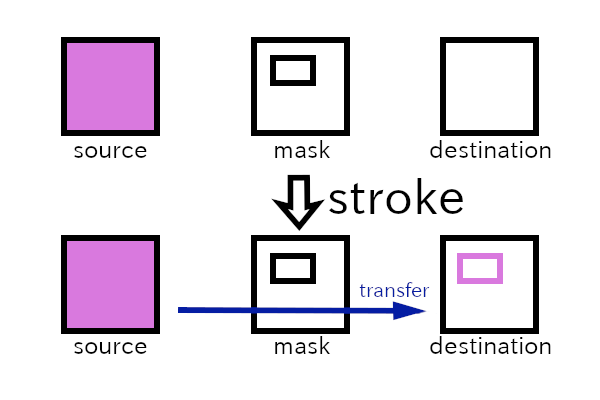
\includegraphics[width=9cm,height=6cm]{../image/cairo.png}
\caption{Stroke a rectangle}
\end{figure}

The instruction is as follows:

\begin{enumerate}
\def\labelenumi{\arabic{enumi}.}
\tightlist
\item
  Create a surface. This will be the destination.
\item
  Create a cairo context with the surface, the surface will be the
  destination of the context.
\item
  Create a source pattern within the context.
\item
  Create paths, which are lines, rectangles, arcs, texts or more
  complicated shapes in the mask.
\item
  Use a drawing operator such as \passthrough{\lstinline!cairo\_stroke!}
  to transfer the paint in the source to the destination.
\item
  Save the destination surface to a file if necessary.
\end{enumerate}

Here's a simple example program that draws a small square and saves it
as a png file. The path of the file is
\passthrough{\lstinline!src/misc/cairo.c!}.

\begin{lstlisting}[language=C, numbers=left]
#include <cairo.h>

int
main (int argc, char **argv)
{
  cairo_surface_t *surface;
  cairo_t *cr;
  int width = 100;
  int height = 100;
  int square_size = 40.0;

  /* Create surface and cairo */
  surface = cairo_image_surface_create (CAIRO_FORMAT_RGB24, width, height);
  cr = cairo_create (surface);

  /* Drawing starts here. */
  /* Paint the background white */
  cairo_set_source_rgb (cr, 1.0, 1.0, 1.0);
  cairo_paint (cr);
  /* Draw a black rectangle */
  cairo_set_source_rgb (cr, 0.0, 0.0, 0.0);
  cairo_set_line_width (cr, 2.0);
  cairo_rectangle (cr,
                   width/2.0 - square_size/2,
                   height/2.0 - square_size/2,
                   square_size,
                   square_size);
  cairo_stroke (cr);

  /* Write the surface to a png file and clean up cairo and surface. */
  cairo_surface_write_to_png (surface, "rectangle.png");
  cairo_destroy (cr);
  cairo_surface_destroy (surface);

  return 0;
}
\end{lstlisting}

\begin{itemize}
\tightlist
\item
  1: Includes the header file of Cairo.
\item
  6: \passthrough{\lstinline!cairo\_surface\_t!} is the type of a
  surface.
\item
  7: \passthrough{\lstinline!cairo\_t!} is the type of a cairo context.
\item
  8-10: \passthrough{\lstinline!width!} and
  \passthrough{\lstinline!height!} are the size of
  \passthrough{\lstinline!surface!}.
  \passthrough{\lstinline!square\_size!} is the size of a square to be
  drawn on the surface.
\item
  13: \passthrough{\lstinline!cairo\_image\_surface\_create!} creates an
  image surface. \passthrough{\lstinline!CAIRO\_FORMAT\_RGB24!} is a
  constant which means that each pixel has red, green and blue data, and
  each data point is an 8 bits number (for 24 bits in total). Modern
  displays have this type of color depth. Width and height are in pixels
  and given as integers.
\item
  14: Creates cairo context. The surface given as an argument will be
  the destination of the context.
\item
  18: \passthrough{\lstinline!cairo\_set\_source\_rgb!} creates a source
  pattern, which is a solid white paint. The second to fourth arguments
  are red, green and blue color values respectively, and they are of
  type float. The values are between zero (0.0) and one (1.0). Black is
  (0.0,0.0,0.0) and white is (1.0,1.0,1.0).
\item
  19: \passthrough{\lstinline!cairo\_paint!} copies everywhere in the
  source to destination. The destination is filled with white pixels
  with this command.
\item
  21: Sets the source color to black.
\item
  22: \passthrough{\lstinline!cairo\_set\_line\_width!} sets the width
  of lines. In this case, the line width is set to be two pixels and
  will end up that same size. (It is because the transformation is
  identity. If the transformation isn't identity, for example scaling
  with the factor three, the actual width in destination will be six
  (2x3=6) pixels.)
\item
  23: Draws a rectangle (square) on the mask. The square is located at
  the center.
\item
  24: \passthrough{\lstinline!cairo\_stroke!} transfers the source to
  destination through the rectangle in the mask.
\item
  31: Outputs the image to a png file
  \passthrough{\lstinline!rectangle.png!}.
\item
  32: Destroys the context. At the same time the source is destroyed.
\item
  33: Destroys the surface.
\end{itemize}

To compile this, change your current directory to
\passthrough{\lstinline!src/misc!} and type the following.

\begin{lstlisting}
$ gcc `pkg-config --cflags cairo` cairo.c `pkg-config --libs cairo`
\end{lstlisting}

s 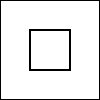
\includegraphics{../image/rectangle.png}

See the \href{https://www.cairographics.org/}{Cairo's website} for
further information.

\subsection{GtkDrawingArea}\label{gtkdrawingarea}

The following is a very simple example.

\begin{lstlisting}[language=C, numbers=left]
#include <gtk/gtk.h>

static void
draw_function (GtkDrawingArea *area, cairo_t *cr, int width, int height, gpointer user_data) {
  int square_size = 40.0;

  cairo_set_source_rgb (cr, 1.0, 1.0, 1.0); /* white */
  cairo_paint (cr);
  cairo_set_line_width (cr, 2.0);
  cairo_set_source_rgb (cr, 0.0, 0.0, 0.0); /* black */
  cairo_rectangle (cr,
                   width/2.0 - square_size/2,
                   height/2.0 - square_size/2,
                   square_size,
                   square_size);
  cairo_stroke (cr);
}

static void
app_activate (GApplication *app, gpointer user_data) {
  GtkWidget *win = gtk_application_window_new (GTK_APPLICATION (app));
  GtkWidget *area = gtk_drawing_area_new ();

  gtk_window_set_title (GTK_WINDOW (win), "da1");
  gtk_drawing_area_set_draw_func (GTK_DRAWING_AREA (area), draw_function, NULL, NULL);
  gtk_window_set_child (GTK_WINDOW (win), area);

  gtk_window_present (GTK_WINDOW (win));
}

#define APPLICATION_ID "com.github.ToshioCP.da1"

int
main (int argc, char **argv) {
  GtkApplication *app;
  int stat;

  app = gtk_application_new (APPLICATION_ID, G_APPLICATION_DEFAULT_FLAGS);
  g_signal_connect (app, "activate", G_CALLBACK (app_activate), NULL);
  stat =g_application_run (G_APPLICATION (app), argc, argv);
  g_object_unref (app);
  return stat;
}
\end{lstlisting}

The function \passthrough{\lstinline!main!} is almost same as before.
The two functions \passthrough{\lstinline!app\_activate!} and
\passthrough{\lstinline!draw\_function!} are important in this example.

\begin{itemize}
\tightlist
\item
  22: Creates a GtkDrawingArea instance.
\item
  25: Sets a drawing function of the widget. GtkDrawingArea widget uses
  the function \passthrough{\lstinline!draw\_function!} to draw the
  contents of itself whenever its necessary. For example, when a user
  drag a mouse pointer and resize a top-level window, GtkDrawingArea
  also changes the size. Then, the whole window needs to be redrawn. For
  the information of
  \passthrough{\lstinline!gtk\_drawing\_area\_set\_draw\_func!}, see
  \href{https://docs.gtk.org/gtk4/method.DrawingArea.set_draw_func.html}{Gtk
  API Reference -- gtk\_drawing\_area\_set\_draw\_func}.
\end{itemize}

The drawing function has five parameters.

\begin{lstlisting}[language=C]
void drawing_function (GtkDrawingArea *drawing_area, cairo_t *cr, int width, int height,
                       gpointer user_data);
\end{lstlisting}

The first parameter is the GtkDrawingArea widget. You can't change any
properties, for example \passthrough{\lstinline!content-width!} or
\passthrough{\lstinline!content-height!}, in this function. The second
parameter is a cairo context given by the widget. The destination
surface of the context is connected to the contents of the widget. What
you draw to this surface will appear in the widget on the screen. The
third and fourth parameters are the size of the destination surface.
Now, look at the program again.

\begin{itemize}
\tightlist
\item
  3-17: The drawing function.
\item
  7-8: Sets the source to be white and paint the destination white.
\item
  9: Sets the line width to be 2.
\item
  10: Sets the source to be black.
\item
  11-15: Adds a rectangle to the mask.
\item
  16: Draws the rectangle with black color to the destination.
\end{itemize}

The program is src/misc/da1.c. Compile and run it, then a window with a
black rectangle (square) appears. Try resizing the window. The square
always appears at the center of the window because the drawing function
is invoked each time the window is resized.

\begin{figure}
\centering
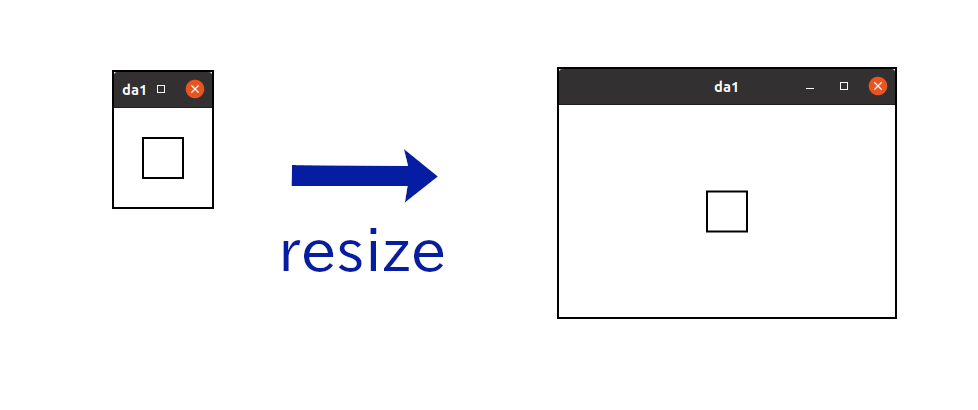
\includegraphics[width=8cm,height=3.4cm]{../image/da1.png}
\caption{Square in the window}
\end{figure}

  \section{Periodic Events}\label{periodic-events}

This chapter was written by Paul Schulz
\href{mailto:paul@mawsonlakes.org}{\nolinkurl{paul@mawsonlakes.org}}.

\subsection{How do we create an
animation?}\label{how-do-we-create-an-animation}

In this section we will continue to build on our previous work. We will
create an analog clock application. By adding a function which
periodically redraws GtkDrawingArea, the clock will be able to
continuously display the time.

The application uses a compiled in `resource' file, so if the GTK4
libraries and their dependencies are installed and available, the
application will run from anywhere.

The program also makes use of some standard mathematical and time
handling functions.

The clocks mechanics were taken from a Cairo drawing example, using
gtkmm4, which can be found
\href{https://developer-old.gnome.org/gtkmm-tutorial/stable/sec-drawing-clock-example.html.en}{here}.

The complete code is at the end.

\subsection{Drawing the clock face, hour, minute and second
hands}\label{drawing-the-clock-face-hour-minute-and-second-hands}

The \passthrough{\lstinline!draw\_clock()!} function does all the work.
See the in-file comments for an explanation of how the Cairo drawing
works.

For a detailed reference of what each of the Cairo functions does see
the
\href{https://www.cairographics.org/manual/cairo-cairo-t.html}{cairo\_t
reference}.

\begin{lstlisting}[language=C, numbers=left]
static void
draw_clock (GtkDrawingArea *area, cairo_t *cr, int width, int height, gpointer user_data) {

    // Scale to unit square and translate (0, 0) to be (0.5, 0.5), i.e.
    // the center of the window
    cairo_scale(cr, width, height);
    cairo_translate(cr, 0.5, 0.5);

    // Set the line width and save the cairo drawing state.
    cairo_set_line_width(cr, m_line_width);
    cairo_save(cr);

    // Set the background to a slightly transparent green.
    cairo_set_source_rgba(cr, 0.337, 0.612, 0.117, 0.9);   // green
    cairo_paint(cr);

    // Resore back to precious drawing state and draw the circular path
    // representing the clockface. Save this state (including the path) so we
    // can reuse it.
    cairo_restore(cr);
    cairo_arc(cr, 0.0, 0.0, m_radius, 0.0, 2.0 * M_PI);
    cairo_save(cr);

    // Fill the clockface with white
    cairo_set_source_rgba(cr, 1.0, 1.0, 1.0, 0.8);
    cairo_fill_preserve(cr);
    // Restore the path, paint the outside of the clock face.
    cairo_restore(cr);
    cairo_stroke_preserve(cr);
    // Set the 'clip region' to the inside of the path (fill region).
    cairo_clip(cr);

    // Clock ticks
    for (int i = 0; i < 12; i++)
    {
        // Major tick size
        double inset = 0.05;

        // Save the graphics state, restore after drawing tick to maintain pen
        // size
        cairo_save(cr);
        cairo_set_line_cap(cr, CAIRO_LINE_CAP_ROUND);

        // Minor ticks are shorter, and narrower.
        if(i % 3 != 0)
        {
            inset *= 0.8;
            cairo_set_line_width(cr, 0.03);
        }

        // Draw tick mark
        cairo_move_to(
            cr,
            (m_radius - inset) * cos (i * M_PI / 6.0),
            (m_radius - inset) * sin (i * M_PI / 6.0));
        cairo_line_to(
            cr,
            m_radius * cos (i * M_PI / 6.0),
            m_radius * sin (i * M_PI / 6.0));
        cairo_stroke(cr);
        cairo_restore(cr); /* stack-pen-size */
    }

    // Draw the analog hands

    // Get the current Unix time, convert to the local time and break into time
    // structure to read various time parts.
    time_t rawtime;
    time(&rawtime);
    struct tm * timeinfo = localtime (&rawtime);

    // Calculate the angles of the hands of our clock
    double hours   = timeinfo->tm_hour * M_PI / 6.0;
    double minutes = timeinfo->tm_min * M_PI / 30.0;
    double seconds = timeinfo->tm_sec * M_PI / 30.0;

    // Save the graphics state
    cairo_save(cr);
    cairo_set_line_cap(cr, CAIRO_LINE_CAP_ROUND);

    cairo_save(cr);

    // Draw the seconds hand
    cairo_set_line_width(cr, m_line_width / 3.0);
    cairo_set_source_rgba(cr, 0.7, 0.7, 0.7, 0.8);   // gray
    cairo_move_to(cr, 0.0, 0.0);
    cairo_line_to(cr,
                  sin(seconds) * (m_radius * 0.9),
                  -cos(seconds) * (m_radius * 0.9));
    cairo_stroke(cr);
    cairo_restore(cr);

    // Draw the minutes hand
    cairo_set_source_rgba(cr, 0.117, 0.337, 0.612, 0.9);   // blue
    cairo_move_to(cr, 0, 0);
    cairo_line_to(cr,
                  sin(minutes + seconds / 60) * (m_radius * 0.8),
                  -cos(minutes + seconds / 60) * (m_radius * 0.8));
    cairo_stroke(cr);

    // draw the hours hand
    cairo_set_source_rgba(cr, 0.337, 0.612, 0.117, 0.9);   // green
    cairo_move_to(cr, 0.0, 0.0);
    cairo_line_to(cr,
                  sin(hours + minutes / 12.0) * (m_radius * 0.5),
                  -cos(hours + minutes / 12.0) * (m_radius * 0.5));
    cairo_stroke(cr);
    cairo_restore(cr);

    // Draw a little dot in the middle
    cairo_arc(cr, 0.0, 0.0, m_line_width / 3.0, 0.0, 2.0 * M_PI);
    cairo_fill(cr);
}
\end{lstlisting}

In order for the clock to be drawn, the drawing function
\passthrough{\lstinline!draw\_clock()!} needs to be registered with
GTK4. This is done in the \passthrough{\lstinline!app\_activate()!}
function (on line 24).

Whenever the application needs to redraw the GtkDrawingArea, it will now
call \passthrough{\lstinline!draw\_clock()!}.

There is still a problem though. In order to animate the clock we need
to also tell the application that the clock needs to be redrawn every
second. This process starts by registering (on the next line, line 15) a
timeout function with \passthrough{\lstinline!g\_timeout\_add()!} that
will wakeup and run another function
\passthrough{\lstinline!time\_handler!}, every second (or 1000ms).

\begin{lstlisting}[language=C, numbers=left]
static void
app_activate (GApplication *app, gpointer user_data) {
    GtkWidget *win;
    GtkWidget *clock;
    GtkBuilder *build;

    build = gtk_builder_new_from_resource ("/com/github/ToshioCP/tfc/tfc.ui");
    win = GTK_WIDGET (gtk_builder_get_object (build, "win"));
    gtk_window_set_application (GTK_WINDOW (win), GTK_APPLICATION (app));

    clock = GTK_WIDGET (gtk_builder_get_object (build, "clock"));
    g_object_unref(build);

    gtk_drawing_area_set_draw_func(GTK_DRAWING_AREA (clock), draw_clock, NULL, NULL);
    g_timeout_add(1000, (GSourceFunc) time_handler, (gpointer) clock);
    gtk_window_present(GTK_WINDOW (win));

}
\end{lstlisting}

Our \passthrough{\lstinline!time\_handler()!} function is very simple,
as it just calls \passthrough{\lstinline!gtk\_widget\_queue\_draw()!}
which schedules a redraw of the widget.

\begin{lstlisting}[language=C, numbers=left]
gboolean
time_handler(GtkWidget* widget) {
    gtk_widget_queue_draw(widget);

    return TRUE;
}
\end{lstlisting}

.. and that is all there is to it. If you compile and run the example
you will get a ticking analog clock.

If you get this working, you can try modifying some of the code in
\passthrough{\lstinline!draw\_clock()!} to tweak the application (such
as change the color or size and length of the hands) or even add text,
or create a digital clock.

\subsection{The Complete code}\label{the-complete-code}

You can find the source files in the \passthrough{\lstinline!tfc!}
directory. it can be compiled with \passthrough{\lstinline!./comp tfc!}.

\passthrough{\lstinline!tfc.c!}

\begin{lstlisting}[language=C, numbers=left]
#include <gtk/gtk.h>
#include <math.h>
#include <time.h>

float m_radius     = 0.42;
float m_line_width = 0.05;

static void
draw_clock (GtkDrawingArea *area, cairo_t *cr, int width, int height, gpointer user_data) {

    // Scale to unit square and translate (0, 0) to be (0.5, 0.5), i.e.
    // the center of the window
    cairo_scale(cr, width, height);
    cairo_translate(cr, 0.5, 0.5);

    // Set the line width and save the cairo drawing state.
    cairo_set_line_width(cr, m_line_width);
    cairo_save(cr);

    // Set the background to a slightly transparent green.
    cairo_set_source_rgba(cr, 0.337, 0.612, 0.117, 0.9);   // green
    cairo_paint(cr);

    // Resore back to precious drawing state and draw the circular path
    // representing the clockface. Save this state (including the path) so we
    // can reuse it.
    cairo_restore(cr);
    cairo_arc(cr, 0.0, 0.0, m_radius, 0.0, 2.0 * M_PI);
    cairo_save(cr);

    // Fill the clockface with white
    cairo_set_source_rgba(cr, 1.0, 1.0, 1.0, 0.8);
    cairo_fill_preserve(cr);
    // Restore the path, paint the outside of the clock face.
    cairo_restore(cr);
    cairo_stroke_preserve(cr);
    // Set the 'clip region' to the inside of the path (fill region).
    cairo_clip(cr);

    // Clock ticks
    for (int i = 0; i < 12; i++)
    {
        // Major tick size
        double inset = 0.05;

        // Save the graphics state, restore after drawing tick to maintain pen
        // size
        cairo_save(cr);
        cairo_set_line_cap(cr, CAIRO_LINE_CAP_ROUND);

        // Minor ticks are shorter, and narrower.
        if(i % 3 != 0)
        {
            inset *= 0.8;
            cairo_set_line_width(cr, 0.03);
        }

        // Draw tick mark
        cairo_move_to(
            cr,
            (m_radius - inset) * cos (i * M_PI / 6.0),
            (m_radius - inset) * sin (i * M_PI / 6.0));
        cairo_line_to(
            cr,
            m_radius * cos (i * M_PI / 6.0),
            m_radius * sin (i * M_PI / 6.0));
        cairo_stroke(cr);
        cairo_restore(cr); /* stack-pen-size */
    }

    // Draw the analog hands

    // Get the current Unix time, convert to the local time and break into time
    // structure to read various time parts.
    time_t rawtime;
    time(&rawtime);
    struct tm * timeinfo = localtime (&rawtime);

    // Calculate the angles of the hands of our clock
    double hours   = timeinfo->tm_hour * M_PI / 6.0;
    double minutes = timeinfo->tm_min * M_PI / 30.0;
    double seconds = timeinfo->tm_sec * M_PI / 30.0;

    // Save the graphics state
    cairo_save(cr);
    cairo_set_line_cap(cr, CAIRO_LINE_CAP_ROUND);

    cairo_save(cr);

    // Draw the seconds hand
    cairo_set_line_width(cr, m_line_width / 3.0);
    cairo_set_source_rgba(cr, 0.7, 0.7, 0.7, 0.8);   // gray
    cairo_move_to(cr, 0.0, 0.0);
    cairo_line_to(cr,
                  sin(seconds) * (m_radius * 0.9),
                  -cos(seconds) * (m_radius * 0.9));
    cairo_stroke(cr);
    cairo_restore(cr);

    // Draw the minutes hand
    cairo_set_source_rgba(cr, 0.117, 0.337, 0.612, 0.9);   // blue
    cairo_move_to(cr, 0, 0);
    cairo_line_to(cr,
                  sin(minutes + seconds / 60) * (m_radius * 0.8),
                  -cos(minutes + seconds / 60) * (m_radius * 0.8));
    cairo_stroke(cr);

    // draw the hours hand
    cairo_set_source_rgba(cr, 0.337, 0.612, 0.117, 0.9);   // green
    cairo_move_to(cr, 0.0, 0.0);
    cairo_line_to(cr,
                  sin(hours + minutes / 12.0) * (m_radius * 0.5),
                  -cos(hours + minutes / 12.0) * (m_radius * 0.5));
    cairo_stroke(cr);
    cairo_restore(cr);

    // Draw a little dot in the middle
    cairo_arc(cr, 0.0, 0.0, m_line_width / 3.0, 0.0, 2.0 * M_PI);
    cairo_fill(cr);
}


gboolean
time_handler(GtkWidget* widget) {
    gtk_widget_queue_draw(widget);

    return TRUE;
}


static void
app_activate (GApplication *app, gpointer user_data) {
    GtkWidget *win;
    GtkWidget *clock;
    GtkBuilder *build;

    build = gtk_builder_new_from_resource ("/com/github/ToshioCP/tfc/tfc.ui");
    win = GTK_WIDGET (gtk_builder_get_object (build, "win"));
    gtk_window_set_application (GTK_WINDOW (win), GTK_APPLICATION (app));

    clock = GTK_WIDGET (gtk_builder_get_object (build, "clock"));
    g_object_unref(build);

    gtk_drawing_area_set_draw_func(GTK_DRAWING_AREA (clock), draw_clock, NULL, NULL);
    g_timeout_add(1000, (GSourceFunc) time_handler, (gpointer) clock);
    gtk_window_present(GTK_WINDOW (win));

}

static void
app_open (GApplication *app, GFile **files, gint n_files, gchar *hint, gpointer user_data) {
    app_activate(app,user_data);
}

int
main (int argc, char **argv) {
    GtkApplication *app;
    int stat;

    app = gtk_application_new ("com.github.ToshioCP.tfc", G_APPLICATION_HANDLES_OPEN);
    g_signal_connect (app, "activate", G_CALLBACK (app_activate), NULL);
    g_signal_connect (app, "open", G_CALLBACK (app_open), NULL);
    stat = g_application_run (G_APPLICATION (app), argc, argv);
    g_object_unref (app);
    return stat;
}
\end{lstlisting}

\passthrough{\lstinline!tfc.ui!}

\begin{lstlisting}[language=XML, numbers=left]
<?xml version="1.0" encoding="UTF-8"?>
<interface>
  <object class="GtkApplicationWindow" id="win">
    <property name="title">Clock</property>
    <property name="default-width">200</property>
    <property name="default-height">200</property>
    <child>
      <object class="GtkDrawingArea" id="clock">
        <property name="hexpand">TRUE</property>
        <property name="vexpand">TRUE</property>
      </object>
    </child>
  </object>
</interface>
\end{lstlisting}

\passthrough{\lstinline!tfc.gresource.xml!}

\begin{lstlisting}[language=XML, numbers=left]
<?xml version="1.0" encoding="UTF-8"?>
<gresources>
  <gresource prefix="/com/github/ToshioCP/tfc">
    <file>tfc.ui</file>
  </gresource>
</gresources>
\end{lstlisting}

\passthrough{\lstinline!comp!}

\begin{lstlisting}[numbers=left]
glib-compile-resources $1.gresource.xml --target=$1.gresource.c --generate-source
gcc `pkg-config --cflags gtk4` $1.gresource.c $1.c `pkg-config --libs gtk4` -lm
\end{lstlisting}

  \section{Custom drawing}\label{custom-drawing}

Custom drawing is to draw shapes dynamically. This section shows an
example of custom drawing. You can draw rectangles by dragging the
mouse.

Down the button.

\begin{figure}
\centering
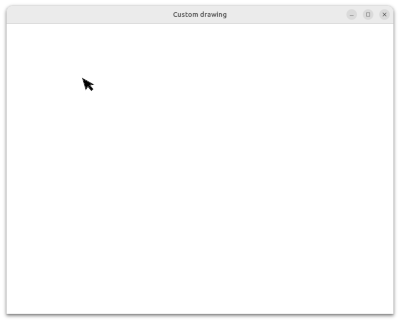
\includegraphics[width=6cm,height=4.83cm]{../image/cd0.png}
\caption{down the button}
\end{figure}

Move the mouse

\begin{figure}
\centering
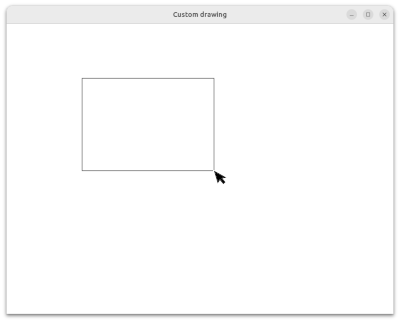
\includegraphics[width=6cm,height=4.83cm]{../image/cd1.png}
\caption{Move the mouse}
\end{figure}

Up the button.

\begin{figure}
\centering
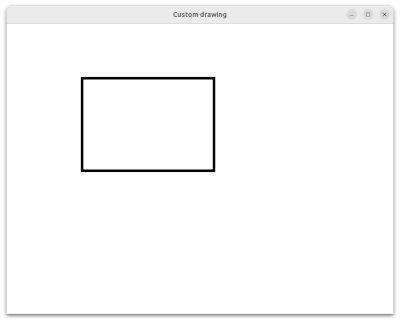
\includegraphics[width=6cm,height=4.83cm]{../image/cd2.png}
\caption{Up the button}
\end{figure}

The programs are at \passthrough{\lstinline!src/custom\_drawing!}
directory. Download the
\href{https://github.com/ToshioCP/Gtk4-tutorial}{repository} and see the
directory. There are four files.

\begin{itemize}
\tightlist
\item
  meson.build
\item
  rect.c
\item
  rect.gresource.xml
\item
  rect.ui
\end{itemize}

\subsection{rect.gresource.xml}\label{rect.gresource.xml}

This file describes a ui file to compile. The compiler
glib-compile-resources uses it.

\begin{lstlisting}[language=XML, numbers=left]
<?xml version="1.0" encoding="UTF-8"?>
<gresources>
  <gresource prefix="/com/github/ToshioCP/rect">
    <file>rect.ui</file>
  </gresource>
</gresources>
\end{lstlisting}

The prefix is \passthrough{\lstinline!/com/github/ToshioCP/rect!} and
the file is \passthrough{\lstinline!rect.ui!}. Therefore, GtkBuilder
reads the resource from
\passthrough{\lstinline!/com/github/ToshioCP/rect/rect.ui!}.

\subsection{rect.ui}\label{rect.ui}

The following is the ui file that defines the widgets. There are two
widgets which are GtkApplicationWindow and GtkDrawingArea. The ids are
\passthrough{\lstinline!win!} and \passthrough{\lstinline!da!}
respectively.

\begin{lstlisting}[language=XML, numbers=left]
<?xml version="1.0" encoding="UTF-8"?>
<interface>
  <object class="GtkApplicationWindow" id="win">
    <property name="default-width">800</property>
    <property name="default-height">600</property>
    <property name="resizable">FALSE</property>
    <property name="title">Custom drawing</property>
    <child>
      <object class="GtkDrawingArea" id="da">
        <property name="hexpand">TRUE</property>
        <property name="vexpand">TRUE</property>
      </object>
    </child>
  </object>
</interface>
\end{lstlisting}

\subsection{rect.c}\label{rect.c}

\subsubsection{GtkApplication}\label{gtkapplication}

This program uses GtkApplication. The application ID is
\passthrough{\lstinline!com.github.ToshioCP.rect!}.

\begin{lstlisting}[language=C]
#define APPLICATION_ID "com.github.ToshioCP.rect"
\end{lstlisting}

See
\href{https://developer.gnome.org/documentation/tutorials/application-id.html}{GNOME
Developer Documentation} for further information.

The function \passthrough{\lstinline!main!} is called at the beginning
of the application.

\begin{lstlisting}[language=C, numbers=left]
int
main (int argc, char **argv) {
  GtkApplication *app;
  int stat;

  app = gtk_application_new (APPLICATION_ID, G_APPLICATION_HANDLES_OPEN);
  g_signal_connect (app, "startup", G_CALLBACK (app_startup), NULL);
  g_signal_connect (app, "activate", G_CALLBACK (app_activate), NULL);
  g_signal_connect (app, "shutdown", G_CALLBACK (app_shutdown), NULL);
  stat =g_application_run (G_APPLICATION (app), argc, argv);
  g_object_unref (app);
  return stat;
}
\end{lstlisting}

It connects three signals and handlers.

\begin{itemize}
\tightlist
\item
  startup: It is emitted after the application is registered to the
  system.
\item
  activate: It is emitted when the application is activated.
\item
  shutdown: It is emitted just before the application quits.
\end{itemize}

\begin{lstlisting}[language=C, numbers=left]
static void
app_startup (GApplication *application) {
  GtkApplication *app = GTK_APPLICATION (application);
  GtkBuilder *build;
  GtkWindow *win;
  GtkDrawingArea *da;
  GtkGesture *drag;

  build = gtk_builder_new_from_resource ("/com/github/ToshioCP/rect/rect.ui");
  win = GTK_WINDOW (gtk_builder_get_object (build, "win"));
  da = GTK_DRAWING_AREA (gtk_builder_get_object (build, "da"));
  gtk_window_set_application (win, app);
  g_object_unref (build);

  gtk_drawing_area_set_draw_func (da, draw_cb, NULL, NULL);
  g_signal_connect_after (da, "resize", G_CALLBACK (resize_cb), NULL);

  drag = gtk_gesture_drag_new ();
  gtk_gesture_single_set_button (GTK_GESTURE_SINGLE (drag), GDK_BUTTON_PRIMARY);
  gtk_widget_add_controller (GTK_WIDGET (da), GTK_EVENT_CONTROLLER (drag));
  g_signal_connect (drag, "drag-begin", G_CALLBACK (drag_begin), NULL);
  g_signal_connect (drag, "drag-update", G_CALLBACK (drag_update), da);
  g_signal_connect (drag, "drag-end", G_CALLBACK (drag_end), da);
}
\end{lstlisting}

The startup handler does three things.

\begin{itemize}
\tightlist
\item
  Builds the widgets.
\item
  Initializes the GtkDrawingArea instance.

  \begin{itemize}
  \tightlist
  \item
    Sets the drawing function
  \item
    Connects the ``resize'' signal and the handler.
  \end{itemize}
\item
  Creates the GtkGestureDrag instance and initializes it. Gesture will
  be explained in this section later.
\end{itemize}

\begin{lstlisting}[language=C, numbers=left]
static void
app_activate (GApplication *application) {
  GtkApplication *app = GTK_APPLICATION (application);
  GtkWindow *win;

  win = gtk_application_get_active_window (app);
  gtk_window_present (win);
}
\end{lstlisting}

The activate handler just shows the window.

\subsubsection{GtkDrawingArea}\label{gtkdrawingarea}

The program has two cairo surfaces and they are pointed by the global
variables.

\begin{lstlisting}[language=C]
static cairo_surface_t *surface = NULL;
static cairo_surface_t *surface_save = NULL;
\end{lstlisting}

The drawing process is as follows.

\begin{itemize}
\tightlist
\item
  Creates an image on \passthrough{\lstinline!surface!}.
\item
  Copies \passthrough{\lstinline!surface!} to the cairo surface of the
  GtkDrawingArea.
\item
  Calls \passthrough{\lstinline!gtk\_widget\_queue\_draw (da)!} to draw
  it if necessary.
\end{itemize}

They are created in the ``resize'' signal handler.

\begin{lstlisting}[language=C, numbers=left]
static void
resize_cb (GtkWidget *widget, int width, int height, gpointer user_data) {
  cairo_t *cr;

  if (surface)
    cairo_surface_destroy (surface);
  surface = cairo_image_surface_create (CAIRO_FORMAT_RGB24, width, height);
  if (surface_save)
    cairo_surface_destroy (surface_save);
  surface_save = cairo_image_surface_create (CAIRO_FORMAT_RGB24, width, height);
  /* Paint the surface white. It is the background color. */
  cr = cairo_create (surface);
  cairo_set_source_rgb (cr, 1.0, 1.0, 1.0);
  cairo_paint (cr);
  cairo_destroy (cr);
}
\end{lstlisting}

This callback is called when the GtkDrawingArea is shown. It is the only
call because the window is not resizable.

It creates image surfaces for \passthrough{\lstinline!surface!} and
\passthrough{\lstinline!surface\_save!}. The
\passthrough{\lstinline!surface!} surface is painted white, which is the
background color.

The drawing function copies \passthrough{\lstinline!surface!} to the
GtkDrawingArea surface.

\begin{lstlisting}[language=C, numbers=left]
static void
draw_cb (GtkDrawingArea *da, cairo_t *cr, int width, int height, gpointer user_data) {
  if (surface) {
    cairo_set_source_surface (cr, surface, 0.0, 0.0);
    cairo_paint (cr);
  }
}
\end{lstlisting}

This function is called by the system when it needs to redraw the
drawing area.

Two surfaces \passthrough{\lstinline!surface!} and
\passthrough{\lstinline!surface\_save!} are destroyed before the
application quits.

\begin{lstlisting}[language=C, numbers=left]
static void
app_shutdown (GApplication *application) {
  if (surface)
    cairo_surface_destroy (surface);
  if (surface_save)
    cairo_surface_destroy (surface_save);
}
\end{lstlisting}

\subsubsection{GtkGestureDrag}\label{gtkgesturedrag}

Gesture class is used to recognize human gestures such as click, drag,
pan, swipe and so on. It is a subclass of GtkEventController. GtkGesture
class is abstract and there are several implementations.

\begin{itemize}
\tightlist
\item
  GtkGestureClick
\item
  GtkGestureDrag
\item
  GtkGesturePan
\item
  GtkGestureSwipe
\item
  other implementations
\end{itemize}

The program \passthrough{\lstinline!rect.c!} uses GtkGestureDrag. It is
the implementation for drags. The parent-child relationship is as
follows.

\begin{lstlisting}
GObject -- GtkEventController -- GtkGesture -- GtkGestureSingle -- GtkGestureDrag
\end{lstlisting}

GtkGestureSingle is a subclass of GtkGesture and optimized for
singe-touch and mouse gestures.

A GtkGestureDrag instance is created and initialized in the startup
signal handler in \passthrough{\lstinline!rect.c!}. See line 18 to 23 in
the following.

\begin{lstlisting}[language=C, numbers=left]
static void
app_startup (GApplication *application) {
  GtkApplication *app = GTK_APPLICATION (application);
  GtkBuilder *build;
  GtkWindow *win;
  GtkDrawingArea *da;
  GtkGesture *drag;

  build = gtk_builder_new_from_resource ("/com/github/ToshioCP/rect/rect.ui");
  win = GTK_WINDOW (gtk_builder_get_object (build, "win"));
  da = GTK_DRAWING_AREA (gtk_builder_get_object (build, "da"));
  gtk_window_set_application (win, app);
  g_object_unref (build);

  gtk_drawing_area_set_draw_func (da, draw_cb, NULL, NULL);
  g_signal_connect_after (da, "resize", G_CALLBACK (resize_cb), NULL);

  drag = gtk_gesture_drag_new ();
  gtk_gesture_single_set_button (GTK_GESTURE_SINGLE (drag), GDK_BUTTON_PRIMARY);
  gtk_widget_add_controller (GTK_WIDGET (da), GTK_EVENT_CONTROLLER (drag));
  g_signal_connect (drag, "drag-begin", G_CALLBACK (drag_begin), NULL);
  g_signal_connect (drag, "drag-update", G_CALLBACK (drag_update), da);
  g_signal_connect (drag, "drag-end", G_CALLBACK (drag_end), da);
}
\end{lstlisting}

\begin{itemize}
\tightlist
\item
  The function \passthrough{\lstinline!gtk\_gesture\_drag\_new!} creates
  a new GtkGestureDrag instance.
\item
  The function
  \passthrough{\lstinline!gtk\_gesture\_single\_set\_button!} sets the
  button number to listen to. The constant
  \passthrough{\lstinline!GDK\_BUTTON\_PRIMARY!} is the left button of a
  mouse.
\item
  The function \passthrough{\lstinline!gtk\_widget\_add\_controller!}
  adds an event controller, gestures are descendants of the event
  controller, to a widget.
\item
  Three signals and handlers are connected.

  \begin{itemize}
  \tightlist
  \item
    drag-begin: Emitted when dragging starts.
  \item
    drag-update: Emitted when the dragging point moves.
  \item
    drag-end: Emitted when the dragging ends.
  \end{itemize}
\end{itemize}

The process during the drag is as follows.

\begin{itemize}
\tightlist
\item
  start: save the surface and start points
\item
  update: restore the surface and draw a thin rectangle between the
  start point and the current point of the mouse
\item
  end: restore the surface and draw a thick rectangle between the start
  and end points.
\end{itemize}

We need two global variables for the start point.

\begin{lstlisting}[language=C]
static double start_x;
static double start_y;
\end{lstlisting}

The following is the handler for the ``drag-begin'' signal.

\begin{lstlisting}[language=C, numbers=left]
static void
copy_surface (cairo_surface_t *src, cairo_surface_t *dst) {
  if (!src || !dst)
    return;
  cairo_t *cr = cairo_create (dst);
  cairo_set_source_surface (cr, src, 0.0, 0.0);
  cairo_paint (cr);
  cairo_destroy (cr);
}

static void
drag_begin (GtkGestureDrag *gesture, double x, double y, gpointer user_data) {
  // save the surface and record (x, y)
  copy_surface (surface, surface_save);
  start_x = x;
  start_y = y;
}
\end{lstlisting}

\begin{itemize}
\tightlist
\item
  Copies \passthrough{\lstinline!surface!} to
  \passthrough{\lstinline!surface\_save!}, which is an image just before
  the dragging.
\item
  Stores the points to \passthrough{\lstinline!start\_x!} and
  \passthrough{\lstinline!start\_y!}.
\end{itemize}

\begin{lstlisting}[language=C, numbers=left]
static void
drag_update  (GtkGestureDrag *gesture, double offset_x, double offset_y, gpointer user_data) {
  GtkWidget *da = GTK_WIDGET (user_data);
  cairo_t *cr;
  
  copy_surface (surface_save, surface);
  cr = cairo_create (surface);
  cairo_rectangle (cr, start_x, start_y, offset_x, offset_y);
  cairo_set_line_width (cr, 1.0);
  cairo_stroke (cr);
  cairo_destroy (cr);
  gtk_widget_queue_draw (da);
}
\end{lstlisting}

\begin{itemize}
\tightlist
\item
  Restores \passthrough{\lstinline!surface!} from
  \passthrough{\lstinline!surface\_save!}.
\item
  Draws a rectangle with thin lines.
\item
  Calls \passthrough{\lstinline!gtk\_widget\_queue\_draw!} to add the
  GtkDrawingArea to the queue to redraw.
\end{itemize}

\begin{lstlisting}[language=C, numbers=left]
static void
drag_end  (GtkGestureDrag *gesture, double offset_x, double offset_y, gpointer user_data) {
  GtkWidget *da = GTK_WIDGET (user_data);
  cairo_t *cr;
  
  copy_surface (surface_save, surface);
  cr = cairo_create (surface);
  cairo_rectangle (cr, start_x, start_y, offset_x, offset_y);
  cairo_set_line_width (cr, 6.0);
  cairo_stroke (cr);
  cairo_destroy (cr);
  gtk_widget_queue_draw (da);
}
\end{lstlisting}

\begin{itemize}
\tightlist
\item
  Restores \passthrough{\lstinline!surface!} from
  \passthrough{\lstinline!surface\_save!}.
\item
  Draws a rectangle with thick lines.
\item
  Calls \passthrough{\lstinline!gtk\_widget\_queue\_draw!} to add the
  GtkDrawingArea to the queue to redraw.
\end{itemize}

\subsection{Build and run}\label{build-and-run}

Download the
\href{https://github.com/ToshioCP/Gtk4-tutorial}{repository}. Change
your current directory to \passthrough{\lstinline!src/custom\_drawing!}.
Run meson and ninja to build the program. Type
\passthrough{\lstinline!\_build/rect!} to run the program. Try to draw
rectangles.

\begin{lstlisting}
$ cd src/custom_drawing
$ meson setup _build
$ ninja -C _build
$ _build/rect
\end{lstlisting}

\begin{figure}
\centering
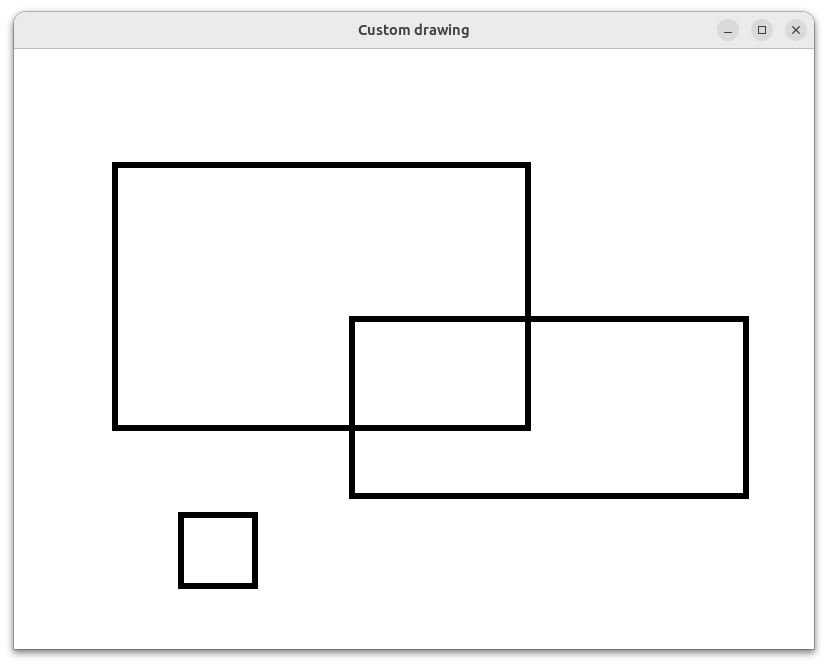
\includegraphics[width=12.4cm,height=10cm]{../image/rect.png}
\caption{The screen of rect program}
\end{figure}

  \section{Tiny turtle graphics
interpreter}\label{tiny-turtle-graphics-interpreter}

A program \passthrough{\lstinline!turtle!} is an example with the
combination of TfeTextView and GtkDrawingArea objects. It is a very
small interpreter but you can draw fractal curves with it. The following
diagram is a Koch curve, which is one of the famous fractal curves.

\begin{figure}
\centering
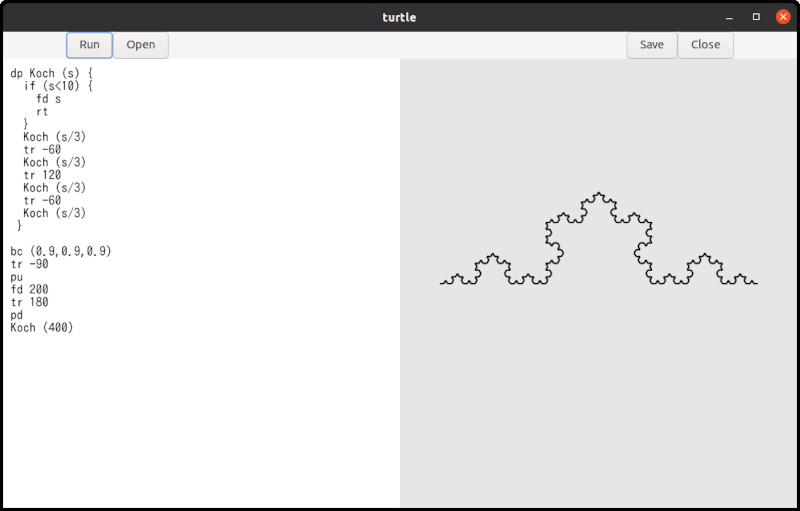
\includegraphics[width=8cm,height=5.11cm]{../src/turtle/image/turtle_koch.png}
\caption{Koch curve}
\end{figure}

The following is a snow-crystal-shaped curve. It is composed of six Koch
curves.

\begin{figure}
\centering
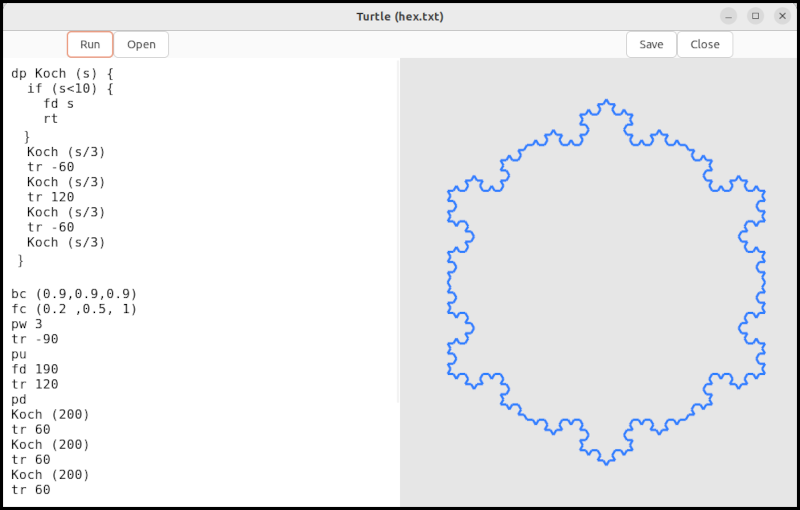
\includegraphics[width=8cm,height=5.11cm]{../image/turtle_snow.png}
\caption{Snow}
\end{figure}

This program uses flex and bison. Flex is a lexical analyzer. Bison is a
parser generator. These two programs are similar to lex and yacc which
are proprietary software developed in Bell Laboratory. However, flex and
bison are open source software. This section describes them and they are
not the topics about GTK 4. So, readers can skip this section.

\subsection{How to use turtle}\label{how-to-use-turtle}

The turtle document is in the appendix. I'll show you a simple example.

\begin{lstlisting}
fc (1,0,0) # Foreground color is red, rgb = (1,0,0).
pd         # Pen down.
rp (4) {   # Repeat four times.
  fd 100   # Go forward by 100 pixels.
  tr 90    # Turn right by 90 degrees.
}
\end{lstlisting}

\begin{enumerate}
\def\labelenumi{\arabic{enumi}.}
\tightlist
\item
  Compile and install \passthrough{\lstinline!turtle!} (See the
  documentation above). Then, run \passthrough{\lstinline!turtle!}.
\item
  Type the program above in the editor (left part of the window).
\item
  Click on the \passthrough{\lstinline!Run!} button, then a red square
  appears on the right part of the window. The side of the square is 100
  pixels long.
\end{enumerate}

In the same way, you can draw other curves. The turtle document includes
some fractal curves such as tree, snow and square-koch. The source codes
are located at src/turtle/example directory. You can read these files
into \passthrough{\lstinline!turtle!} editor by clicking on the
\passthrough{\lstinline!Open!} button.

\subsection{Combination of TfeTextView and GtkDrawingArea
objects}\label{combination-of-tfetextview-and-gtkdrawingarea-objects}

Turtle uses TfeTextView and GtkDrawingArea.

\begin{enumerate}
\def\labelenumi{\arabic{enumi}.}
\tightlist
\item
  A user inputs/reads a turtle program into the buffer in the
  TfeTextView instance.
\item
  The user clicks on the ``Run'' button.
\item
  The parser reads the program and generates tree-structured data.
\item
  The interpriter reads the data and executes it step by step. And it
  draws shapes on a surface. The surface isn't the one in the
  GtkDrawingArea widget.
\item
  The widget is added to the queue. It will be redrawn with the drawing
  function, which just copies the surface into the one in the
  GtkDrawingArea.
\end{enumerate}

\begin{figure}
\centering
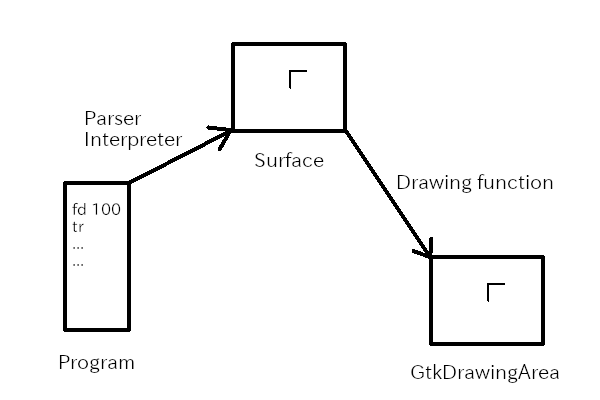
\includegraphics{../image/turtle.png}
\caption{Parser, interpreter and drawing function}
\end{figure}

The body of the interpreter is written with flex and bison. The codes
are not thread safe. So the callback function
\passthrough{\lstinline!run\_cb!}, which is the handler of ``clicked''
signal on the \passthrough{\lstinline!Run!} button, prevents reentering.

\begin{lstlisting}[language=C, numbers=left]
void
run_cb (GtkWidget *btnr) {
  GtkTextBuffer *tb = gtk_text_view_get_buffer (GTK_TEXT_VIEW (tv));
  GtkTextIter start_iter;
  GtkTextIter end_iter;
  char *contents;
  int stat;
  static gboolean busy = FALSE; /* initialized only once */
  cairo_t *cr;

  /* yyparse() and run() are NOT thread safe. */
  /* The variable busy avoids reentrance. */
  if (busy)
    return;
  busy = TRUE;
  gtk_text_buffer_get_bounds (tb, &start_iter, &end_iter);
  contents = gtk_text_buffer_get_text (tb, &start_iter, &end_iter, FALSE);
  if (surface && contents[0] != '\0') {
    init_flex (contents);
    stat = yyparse ();
    if (stat == 0) { /* No error */
      run ();
    }
    finalize_flex ();
  } else if (surface) {
    cr = cairo_create (surface);
    cairo_set_source_rgb (cr, 1.0, 1.0, 1.0);
    cairo_paint (cr);
    cairo_destroy (cr);
  }
  g_free (contents);
  gtk_widget_queue_draw (GTK_WIDGET (da));
  busy = FALSE;
}

static void
resize_cb (GtkDrawingArea *drawing_area, int width, int height, gpointer user_data) {

  if (surface)
    cairo_surface_destroy (surface);
  surface = cairo_image_surface_create (CAIRO_FORMAT_ARGB32, width, height);
  run_cb (NULL); // NULL is a fake (run button).
}
\end{lstlisting}

\begin{itemize}
\tightlist
\item
  8, 13-15: The static value \passthrough{\lstinline!busy!} holds a
  status of the interpreter. If it is \passthrough{\lstinline!TRUE!},
  the interpreter is running and it is not possible to call the
  interpreter because it's not a re-entrant program. If it is
  \passthrough{\lstinline!FALSE!}, it is safe to call the interpreter
  and set the variable \passthrough{\lstinline!busy!} to TRUE.
\item
  16-17: Gets the contents of \passthrough{\lstinline!tb!}.
\item
  18-30: The variable \passthrough{\lstinline!surface!} is a static
  variable. It points to a \passthrough{\lstinline!cairo\_surface\_t!}
  instance. It is created when the GtkDrawingArea instance is realized
  and whenever it is resized. Therefore,
  \passthrough{\lstinline!surface!} isn't NULL usually. But if it is
  NULL, the interpreter won't be called.
\item
  18-24: If \passthrough{\lstinline!surface!} points a surface instance
  and the string \passthrough{\lstinline!contents!} isn't empty, it
  calls the interpreter.

  \begin{itemize}
  \tightlist
  \item
    Initializes the lexical analyzer.
  \item
    Calls the parser. The parser analyzes the program codes
    syntactically and generates a tree structured data.
  \item
    If the parser successfully parsed, it calls the runtime routine
    `run'.
  \item
    Finalizes the lexical analyzer.
  \end{itemize}
\item
  25-29: If \passthrough{\lstinline!surface!} points a surface instance
  and the string \passthrough{\lstinline!contents!} is empty, it clears
  the surface \passthrough{\lstinline!surface!}.
\item
  31: Frees \passthrough{\lstinline!contents!}.
\item
  32: Adds the drawing area widget to the queue to draw.
\item
  33: Sets the variable \passthrough{\lstinline!busy!} to FALSE.
\item
  36-43: The ``resized'' signal handler. If the
  \passthrough{\lstinline!surface!} isn't NULL, it is destroyed. A new
  surface is created. Its size is the same as the surface of the
  GtkDrawingArea instance. It calls the callback function
  \passthrough{\lstinline!run\_cb!} to redraw the shape on the drawing
  area.
\end{itemize}

If the open button is clicked and a file is read, the filename will be
shown on the header bar.

\begin{lstlisting}[language=C, numbers=left]
static void
show_filename (TfeTextView *tv) {
  GFile *file;
  char *filename;
  char *title;

  file = tfe_text_view_get_file (tv);
  if (G_IS_FILE (file)) {
    filename = g_file_get_basename (file);
    title = g_strdup_printf ("Turtle (%s)", filename);
    g_free (filename);
    g_object_unref (file);
  } else
    title = g_strdup ("Turtle");
  gtk_window_set_title (GTK_WINDOW (win), title);
  g_free (title);
}
\end{lstlisting}

This function is the callback function of the ``change-file'' signal on
the TfeTextView instance. It calls
\passthrough{\lstinline!tfe\_text\_view\_get\_file!}.

\begin{itemize}
\tightlist
\item
  If the return value is a GFile instance, the title will be ``Turtle
  (the filename)''.
\item
  Otherwise, the title will be ``Turtle''.
\end{itemize}

Other part of \passthrough{\lstinline!turtleapplication.c!} is very
simple and similar to the codes in the former applications. The codes of
\passthrough{\lstinline!turtleapplication.c!} is in the turtle
directory.

\subsection{What does the interpreter
do?}\label{what-does-the-interpreter-do}

Suppose that the turtle application runs with the following program.

\begin{lstlisting}
distance = 100
fd distance*2
\end{lstlisting}

The application recognizes the program and works as follows.

\begin{itemize}
\tightlist
\item
  Generally, a program consists of tokens. Tokens are ``distance'',
  ``='', ``100'', ``fd'', ``*'' and ``2'' in the above example..
\item
  The parser calls a function \passthrough{\lstinline!yylex!} to read a
  token in the source file. \passthrough{\lstinline!yylex!} returns a
  code which is called ``token kind'' and sets a global variable
  \passthrough{\lstinline!yylval!} to a value, which is called a
  semantic value. The type of \passthrough{\lstinline!yylval!} is union.
  The type of \passthrough{\lstinline!yylval.ID!} and
  \passthrough{\lstinline!yylval.NUM!} are string and double
  respectively. There are seven tokens in the program so
  \passthrough{\lstinline!yylex!} is called seven times.
\end{itemize}

\begin{longtable}[]{@{}cccc@{}}
\toprule\noalign{}
& token kind & yylval.ID & yylval.NUM \\
\midrule\noalign{}
\endhead
\bottomrule\noalign{}
\endlastfoot
1 & ID & distance & \\
2 & = & & \\
3 & NUM & & 100 \\
4 & FD & & \\
5 & ID & distance & \\
6 & * & & \\
7 & NUM & & 2 \\
\end{longtable}

\begin{itemize}
\tightlist
\item
  The function \passthrough{\lstinline!yylex!} returns a token kind
  every time, but it doesn't set \passthrough{\lstinline!yylval.ID!} or
  \passthrough{\lstinline!yylval.NUM!} every time. It is because
  keywords (\passthrough{\lstinline!FD!}) and symbols
  (\passthrough{\lstinline!=!} and \passthrough{\lstinline!*!}) don't
  have any semantic values. The function \passthrough{\lstinline!yylex!}
  is called lexical analyzer or scanner.
\item
  The application \passthrough{\lstinline!turtle!} makes a tree
  structured data. This part of \passthrough{\lstinline!turtle!} is
  called parser.
\end{itemize}

\begin{figure}
\centering
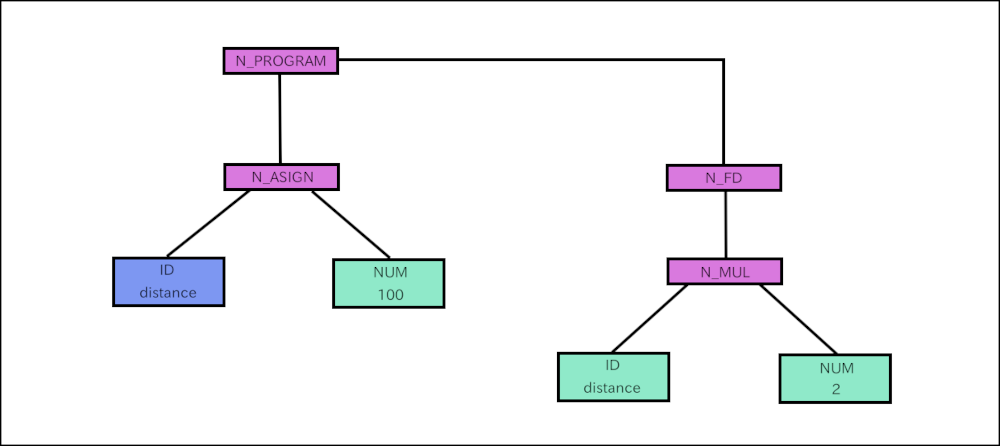
\includegraphics[width=12cm,height=5.34cm]{../image/turtle_parser_tree.png}
\caption{turtle parser tree}
\end{figure}

\begin{itemize}
\tightlist
\item
  \passthrough{\lstinline!Turtle!} analyzes the tree and executes it.
  This part of \passthrough{\lstinline!turtle!} is called runtime
  routine or interpreter. The tree consists of rectangles and line
  segments between the rectangles. The rectangles are called nodes. For
  example, N\_PROGRAM, N\_ASSIGN, N\_FD and N\_MUL are nodes.

  \begin{enumerate}
  \def\labelenumi{\arabic{enumi}.}
  \tightlist
  \item
    Goes down from N\_PROGRAM to N\_ASSIGN.
  \item
    N\_ASSIGN node has two children, ID and NUM. This node comes from
    ``distance = 100'' which is ``ID = NUM'' syntactically. First,
    \passthrough{\lstinline!turtle!} checks if the first child is ID. If
    it's ID, then \passthrough{\lstinline!turtle!} looks for the
    variable in the variable table. If it doesn't exist, it registers
    the ID (\passthrough{\lstinline!distance!}) to the table. Then go
    back to the N\_ASSIGN node.
  \item
    \passthrough{\lstinline!Turtle!} calculates the second child. In
    this case its a number 100. Saves 100 to the variable table at the
    \passthrough{\lstinline!distance!} record.
  \item
    \passthrough{\lstinline!Turtle!} goes back to N\_PROGRAM then go to
    the next node N\_FD. It has only one child. Goes down to the child
    N\_MUL.
  \item
    The first child is ID (distance). Searches the variable table for
    the variable \passthrough{\lstinline!distance!} and gets the value
    100. The second child is a number 2. Multiplies 100 by 2 and gets
    200. Then \passthrough{\lstinline!turtle!} goes back to N\_FD.
  \item
    Now \passthrough{\lstinline!turtle!} knows the distance is 200. It
    moves the cursor forward by 200 pixels. The segment is drawn on the
    \passthrough{\lstinline!surface!}.
  \item
    There are no node follows. Runtime routine returns to the function
    \passthrough{\lstinline!run\_cb!}.
  \end{enumerate}
\item
  The function \passthrough{\lstinline!run\_cb!} calls
  \passthrough{\lstinline!gtk\_widget\_queue\_draw!} and put the
  GtkDrawingArea widget to the queue.
\item
  The system redraws the widget. At that time drawing function
  \passthrough{\lstinline!draw\_func!} is called. The function copies
  the \passthrough{\lstinline!surface!} to the surface in the
  GtkDrawingArea.
\end{itemize}

Actual turtle program is more complicated than the example above.
However, what turtle does is basically the same. Interpretation consists
of three parts.

\begin{itemize}
\tightlist
\item
  Lexical analysis
\item
  Syntax Parsing and tree generation
\item
  Interpretation and execution of the tree.
\end{itemize}

\subsection{Compilation flow}\label{compilation-flow}

The source files are:

\begin{itemize}
\tightlist
\item
  flex source file =\textgreater{} \passthrough{\lstinline!turtle.lex!}
\item
  bison source file =\textgreater{} \passthrough{\lstinline!turtle.y!}
\item
  C header file =\textgreater{} \passthrough{\lstinline!turtle\_lex.h!}
\item
  C source file =\textgreater{}
  \passthrough{\lstinline!turtleapplication.c!}
\item
  other files =\textgreater{} \passthrough{\lstinline!turtle.ui!},
  \passthrough{\lstinline!turtle.gresources.xml!} and
  \passthrough{\lstinline!meson.build!}
\end{itemize}

The compilation process is a bit complicated.

\begin{enumerate}
\def\labelenumi{\arabic{enumi}.}
\tightlist
\item
  glib-compile-resources compiles \passthrough{\lstinline!turtle.ui!} to
  \passthrough{\lstinline!resources.c!} according to
  \passthrough{\lstinline!turtle.gresource.xml!}. It also generates
  \passthrough{\lstinline!resources.h!}.
\item
  bison compiles \passthrough{\lstinline!turtle.y!} to
  \passthrough{\lstinline!turtle\_parser.c!} and generates
  \passthrough{\lstinline!turtle\_parser.h!}
\item
  flex compiles \passthrough{\lstinline!turtle.lex!} to
  \passthrough{\lstinline!turtle\_lex.c!}.
\item
  gcc compiles \passthrough{\lstinline!application.c!},
  \passthrough{\lstinline!resources.c!},
  \passthrough{\lstinline!turtle\_parser.c!} and
  \passthrough{\lstinline!turtle\_lex.c!} with
  \passthrough{\lstinline!turtle\_lex.h!},
  \passthrough{\lstinline!resources.h!} and
  \passthrough{\lstinline!turtle\_parser.h!}. It generates an executable
  file \passthrough{\lstinline!turtle!}.
\end{enumerate}

\begin{figure}
\centering
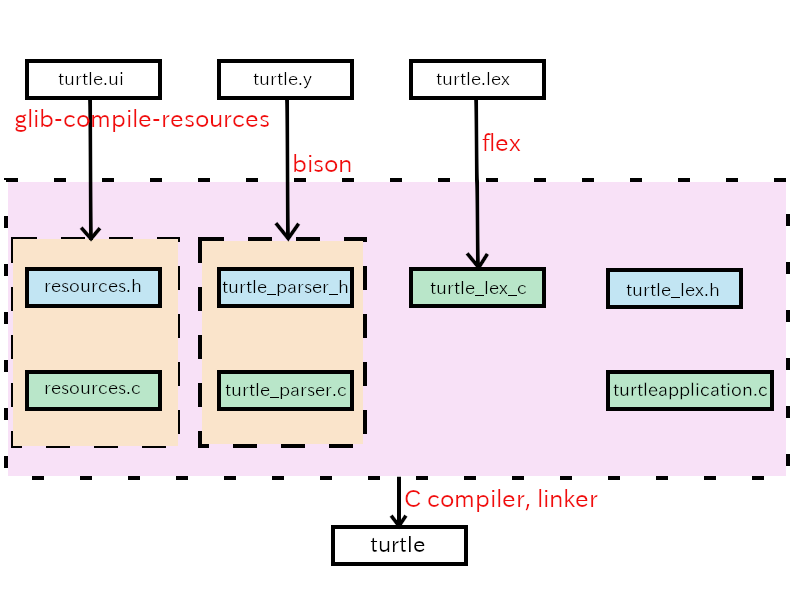
\includegraphics[width=12cm,height=9cm]{../image/turtle_compile_process.png}
\caption{compile process}
\end{figure}

Meson controls the process. The instruction is described in
\passthrough{\lstinline!meson.build!}.

\begin{lstlisting}[numbers=left]
project('turtle', 'c')

compiler = meson.get_compiler('c')
mathdep = compiler.find_library('m', required : true)

gtkdep = dependency('gtk4')

gnome=import('gnome')
resources = gnome.compile_resources('resources','turtle.gresource.xml')

flex = find_program('flex')
bison = find_program('bison')
turtleparser = custom_target('turtleparser', input: 'turtle.y', output: ['turtle_parser.c', 'turtle_parser.h'], command: [bison, '-d', '-o', 'turtle_parser.c', '@INPUT@'])
turtlelexer = custom_target('turtlelexer', input: 'turtle.lex', output: 'turtle_lex.c', command: [flex, '-o', '@OUTPUT@', '@INPUT@'])

sourcefiles=files('turtleapplication.c', '../tfetextview/tfetextview.c')

executable('turtle', sourcefiles, resources, turtleparser, turtlelexer, turtleparser[1], dependencies: [mathdep, gtkdep], export_dynamic: true, install: true)
\end{lstlisting}

\begin{itemize}
\tightlist
\item
  1: The project name is ``turtle'' and the program language is C.
\item
  3: Gets C compiler. It is usually \passthrough{\lstinline!gcc!} in
  linux.
\item
  4: Gets math library. This program uses trigonometric functions. They
  are defined in the math library, but the library is optional. So, it
  is necessary to include it by
  \passthrough{\lstinline!\#include <math.h>!} and also link the library
  with the linker.
\item
  6: Gets gtk4 library.
\item
  8: Gets gnome module.See
  \href{https://mesonbuild.com/Gnome-module.html\#gnome-module}{Meson
  build system website -- GNOME module} for further information.
\item
  9: Compiles ui file to C source file according to the XML file
  \passthrough{\lstinline!turtle.gresource.xml!}.
\item
  11: Gets flex.
\item
  12: Gets bison.
\item
  13: Compiles \passthrough{\lstinline!turtle.y!} to
  \passthrough{\lstinline!turtle\_parser.c!} and
  \passthrough{\lstinline!turtle\_parser.h!} by bison. The function
  \passthrough{\lstinline!custom\_target!} creates a custom top level
  target. See
  \href{https://mesonbuild.com/Reference-manual_functions.html\#custom_target}{Meson
  build system website -- custom target} for further information.
\item
  14: Compiles \passthrough{\lstinline!turtle.lex!} to
  \passthrough{\lstinline!turtle\_lex.c!} by flex.
\item
  16: The variable \passthrough{\lstinline!sourcefiles!} is a file
  object created with the C source files.
\item
  18: Compiles C source files including generated files by
  glib-compile-resources, bison and flex. The argument
  \passthrough{\lstinline!turtleparser[1]!} refers to
  \passthrough{\lstinline!tirtle\_parser.h!} which is the second output
  in the line 13.
\end{itemize}

\subsection{Turtle.lex}\label{turtle.lex}

\subsubsection{What does flex do?}\label{what-does-flex-do}

Flex creates lexical analyzer from flex source file. Flex source file is
a text file. Its syntactic rule will be explained later. Generated
lexical analyzer is a C source file. It is also called scanner. It reads
a text file, which is a source file of a program language, and gets
variable names, numbers and symbols. Suppose here is a turtle source
file.

\begin{lstlisting}
fc (1,0,0) # Foreground color is red, rgb = (1,0,0).
pd         # Pen down.
distance = 100
angle = 90
fd distance    # Go forward by distance (100) pixels.
tr angle     # Turn right by angle (90) degrees.
\end{lstlisting}

The content of the text file is separated into
\passthrough{\lstinline!fc!}, \passthrough{\lstinline!(!},
\passthrough{\lstinline!1!} and so on. The words
\passthrough{\lstinline!fc!}, \passthrough{\lstinline!pd!},
\passthrough{\lstinline!distance!}, \passthrough{\lstinline!angle!},
\passthrough{\lstinline!tr!}, \passthrough{\lstinline!1!},
\passthrough{\lstinline!0!}, \passthrough{\lstinline!100!} and
\passthrough{\lstinline!90!} are called tokens. The characters
`\passthrough{\lstinline!(!}' (left parenthesis),
`\passthrough{\lstinline!,!}' (comma), `\passthrough{\lstinline!)!}'
(right parenthesis) and `\passthrough{\lstinline!=!}' (equal sign) are
called symbols. ( Sometimes those symbols called tokens, too.)

Flex reads \passthrough{\lstinline!turtle.lex!} and generates the C
source file of a scanner. The file \passthrough{\lstinline!turtle.lex!}
specifies tokens, symbols and the behavior which corresponds to each
token or symbol. Turtle.lex isn't a big program.

\begin{lstlisting}[numbers=left]
%top{
#include <string.h>
#include <stdlib.h>
#include <glib.h>
#include "turtle_parser.h"

  static int nline = 1;
  static int ncolumn = 1;
  static void get_location (char *text);

  /* Dinamically allocated memories are added to the single list. They will be freed in the finalize function. */
  extern GSList *list;
}

%option noyywrap

REAL_NUMBER (0|[1-9][0-9]*)(\.[0-9]+)?
IDENTIFIER [a-zA-Z][a-zA-Z0-9]*
%%
  /* rules */
#.*               ; /* comment. Be careful. Dot symbol (.) matches any character but new line. */
[ ]               ncolumn++; /* white space. [ and ] is a "character class". */
\t                ncolumn += 8; /* assume that tab is 8 spaces. */
\n                nline++; ncolumn = 1;
  /* reserved keywords */
pu                get_location (yytext); return PU; /* pen up */
pd                get_location (yytext); return PD; /* pen down */
pw                get_location (yytext); return PW; /* pen width = line width */
fd                get_location (yytext); return FD; /* forward */
tr                get_location (yytext); return TR; /* turn right */
tl                get_location (yytext); return TL; /* turn left, since ver 0.5 */
bc                get_location (yytext); return BC; /* background color */
fc                get_location (yytext); return FC; /* foreground color */
dp                get_location (yytext); return DP; /* define procedure */
if                get_location (yytext); return IF; /* if statement */
rt                get_location (yytext); return RT; /* return statement */
rs                get_location (yytext); return RS; /* reset the status */
rp                get_location (yytext); return RP; /* repeat, since ver 0.5 */
  /* constant */
{REAL_NUMBER}     get_location (yytext); yylval.NUM = atof (yytext); return NUM;
  /* identifier */
{IDENTIFIER}      { get_location (yytext); yylval.ID = g_strdup(yytext);
                    list = g_slist_prepend (list, yylval.ID);
                    return ID;
                  }
"="               get_location (yytext); return '=';
">"               get_location (yytext); return '>';
"<"               get_location (yytext); return '<';
"+"               get_location (yytext); return '+';
"-"               get_location (yytext); return '-';
"*"               get_location (yytext); return '*';
"/"               get_location (yytext); return '/';
"("               get_location (yytext); return '(';
")"               get_location (yytext); return ')';
"{"               get_location (yytext); return '{';
"}"               get_location (yytext); return '}';
","               get_location (yytext); return ',';
.                 ncolumn++;             return YYUNDEF;
%%

static void
get_location (char *text) {
  yylloc.first_line = yylloc.last_line = nline;
  yylloc.first_column = ncolumn;
  yylloc.last_column = (ncolumn += strlen(text)) - 1;
}

static YY_BUFFER_STATE state;

void
init_flex (const char *text) {
  state = yy_scan_string (text);
}

void
finalize_flex (void) {
  yy_delete_buffer (state);
}
\end{lstlisting}

The file consists of three sections which are separated by ``\%\%''
(line 19 and 59). They are definitions, rules and user code sections.

\subsubsection{Definitions section}\label{definitions-section}

\begin{itemize}
\tightlist
\item
  1-12: Lines between ``\%top\{'' and ``\}'' are C source codes. They
  will be copied to the top of the generated C source file.
\item
  2-3: This program uses two functions \passthrough{\lstinline!strlen!}
  (l.65) and \passthrough{\lstinline!atof!} (l.40). They are defined in
  \passthrough{\lstinline!string.h!} and
  \passthrough{\lstinline!stdlib.h!} respectively. These two header
  files are included here.
\item
  4: This program uses some GLib functions and structures like
  \passthrough{\lstinline!g\_strdup!} and
  \passthrough{\lstinline!GSList!}. GLib header file is
  \passthrough{\lstinline!glib.h!} and it is included here.
\item
  5: The header file ``turtle\_parser.h'' is generated from ``turtle.y''
  by bison. It defines some constants and functions like
  \passthrough{\lstinline!PU!} and \passthrough{\lstinline!yylloc!}. The
  header file is included here.
\item
  7-9: The current input position is pointed by
  \passthrough{\lstinline!nline!} and \passthrough{\lstinline!ncolumn!}.
  The function \passthrough{\lstinline!get\_location!} is declared here
  so that it can be called before the function is defined (l.61-65).
\item
  12: GSlist is a structure for a singly-linked list. The variable
  \passthrough{\lstinline!list!} is defined in
  \passthrough{\lstinline!turtle.y!} so its class is
  \passthrough{\lstinline!extern!}. It is the start point of the list.
  The list is used to keep allocated memories.
\item
  15: This option \passthrough{\lstinline!\%option noyywrap!} must be
  specified when you have only single source file to the scanner. Refer
  to ``9 The Generated Scanner'' in the flex documentation in your
  distribution. (The documentation is not on the internet.)
\item
  17-18: \passthrough{\lstinline!REAL\_NUMBER!} and
  \passthrough{\lstinline!IDENTIFIER!} are names. A name begins with a
  letter or an underscore followed by zero or more letters, digits,
  underscores (\passthrough{\lstinline!\_!}) or dashes
  (\passthrough{\lstinline!-!}). They are followed by regular
  expressions which are their definitions. They will be used in rules
  section and will expand to the definition.
\end{itemize}

\subsubsection{Rules section}\label{rules-section}

This section is the most important part. Rules consist of patterns and
actions. The patterns are regular expressions or names surrounded by
braces. The names must be defined in the definitions section. The
definition of the regular expression is written in the flex
documentation.

For example, line 40 is a rule.

\begin{itemize}
\tightlist
\item
  \passthrough{\lstinline!\{REAL\_NUMBER\}!} is a pattern
\item
  \passthrough{\lstinline!get\_location (yytext); yylval.NUM = atof (yytext); return NUM;!}
  is an action.
\end{itemize}

\passthrough{\lstinline!\{REAL\_NUMBER\}!} is defined in the line 17, so
it expands to \passthrough{\lstinline!(0|[1-9][0-9]*)(\\.[0-9]+)?!}.
This regular expression matches numbers like
\passthrough{\lstinline!0!}, \passthrough{\lstinline!12!} and
\passthrough{\lstinline!1.5!}. If an input is a number, it matches the
pattern in line 40. Then the matched text is assigned to
\passthrough{\lstinline!yytext!} and corresponding action is executed. A
function \passthrough{\lstinline!get\_location!} changes the location
variables to the position at the text. It assigns
\passthrough{\lstinline!atof (yytext)!}, which is double sized number
converted from \passthrough{\lstinline!yytext!}, to
\passthrough{\lstinline!yylval.NUM!} and return
\passthrough{\lstinline!NUM!}. \passthrough{\lstinline!NUM!} is a token
kind and it represents (double type) numbers. It is defined in
\passthrough{\lstinline!turtle.y!}.

The scanner generated by flex has \passthrough{\lstinline!yylex!}
function. If \passthrough{\lstinline!yylex!} is called and the input is
``123.4'', then it works as follows.

\begin{enumerate}
\def\labelenumi{\arabic{enumi}.}
\tightlist
\item
  A string ``123.4'' matches \passthrough{\lstinline!\{REAL\_NUMBER\}!}.
\item
  Updates the location variable \passthrough{\lstinline!ncolumn!}. The
  structure \passthrough{\lstinline!yylloc!} is set by
  \passthrough{\lstinline!get\_location!}.
\item
  The function \passthrough{\lstinline!atof!} converts the string
  ``123.4'' to double type number 123.4.
\item
  It is assigned to \passthrough{\lstinline!yylval.NUM!}.
\item
  \passthrough{\lstinline!yylex!} returns \passthrough{\lstinline!NUM!}
  to the caller.
\end{enumerate}

Then the caller knows the input is a number
(\passthrough{\lstinline!NUM!}), and its value is 123.4.

\begin{itemize}
\tightlist
\item
  20-58: Rules section.
\item
  21: The symbol \passthrough{\lstinline!.!} (dot) matches any character
  except newline. Therefore, a comment begins
  \passthrough{\lstinline!\#!} followed by any characters except
  newline. No action happens. That means that comments are ignored.
\item
  22: White space just increases the variable
  \passthrough{\lstinline!ncolumn!} by one.
\item
  23: Tab is assumed to be equal to eight spaces.
\item
  24: New line increases a variable \passthrough{\lstinline!nline!} by
  one and resets \passthrough{\lstinline!ncolumn!}.
\item
  26-38: Keywords updates the location variables
  \passthrough{\lstinline!ncolumn!} and
  \passthrough{\lstinline!yylloc!}, and returns the token kinds of the
  keywords.
\item
  40: Real number constant. The action converts the
  text\passthrough{\lstinline!yytext!} to a double type number, puts it
  into \passthrough{\lstinline!yylval.NUM!} and returns
  \passthrough{\lstinline!NUM!}.
\item
  42: \passthrough{\lstinline!IDENTIFIER!} is defined in line 18. The
  identifier is a name of variable or procedure. It begins with a letter
  and followed by letters or digits. The location variables are updated
  and the name of the identifier is assigned to
  \passthrough{\lstinline!yylval.ID!}. The memory of the name is
  allocated by the function \passthrough{\lstinline!g\_strdup!}. The
  memory is registered to the list (GSlist type list). The memory will
  be freed after the runtime routine finishes. A token kind
  \passthrough{\lstinline!ID!} is returned.
\item
  46-57: Symbols update the location variable and return the token
  kinds. The token kind is the same as the symbol itself.
\item
  58: If the input doesn't match the patterns, then it is an error. A
  special token kind \passthrough{\lstinline!YYUNDEF!} is returned.
\end{itemize}

\subsubsection{User code section}\label{user-code-section}

This section is just copied to C source file.

\begin{itemize}
\tightlist
\item
  61-66: A function \passthrough{\lstinline!get\_location!}. The
  location of the input is recorded to \passthrough{\lstinline!nline!}
  and \passthrough{\lstinline!ncolumn!}. A variable
  \passthrough{\lstinline!yylloc!} is referred by the parser. It is a C
  structure and has four members, \passthrough{\lstinline!first\_line!},
  \passthrough{\lstinline!first\_column!},
  \passthrough{\lstinline!last\_line!} and
  \passthrough{\lstinline!last\_column!}. They point the start and end
  of the current input text.
\item
  68: \passthrough{\lstinline!YY\_BUFFER\_STATE!} is a pointer points
  the input buffer. Flex makes the definition of
  \passthrough{\lstinline!YY\_BUFFER\_STATE!} in the C file (scanner
  source file \passthrough{\lstinline!turtle\_lex.c!}). See your flex
  document, section 11 Multiple Input Buffers, for further information.
\item
  70-73: A function \passthrough{\lstinline!init\_flex!} is called by
  \passthrough{\lstinline!run\_cb!} which is a ``clicked'' signal
  handler on the \passthrough{\lstinline!Run!} button. It has one string
  type parameter. The caller assigns it with the content of the
  GtkTextBuffer instance. A function
  \passthrough{\lstinline!yy\_scan\_string!} sets the input buffer for
  the scanner.
\item
  75-78: A function \passthrough{\lstinline!finalize\_flex!} is called
  after runtime routine finishes. It deletes the input buffer.
\end{itemize}

\subsection{Turtle.y}\label{turtle.y}

Turtle.y has more than 800 lines so it is difficult to explain all the
source code. So I will explain the key points and leave out other less
important parts.

\subsubsection{What does bison do?}\label{what-does-bison-do}

Bison creates C source file of a parser from a bison source file. The
bison source file is a text file. A parser analyzes a program source
code according to its grammar. Suppose here is a turtle source file.

\begin{lstlisting}
fc (1,0,0) # Foreground color is red, rgb = (1,0,0).
pd         # Pen down.
distance = 100
angle = 90
fd distance    # Go forward by distance (100) pixels.
tr angle     # Turn right by angle (90) degrees.
\end{lstlisting}

The parser calls \passthrough{\lstinline!yylex!} to get a token. The
token consists of its type (token kind) and value (semantic value). So,
the parser gets items in the following table whenever it calls
\passthrough{\lstinline!yylex!}.

\begin{longtable}[]{@{}cccc@{}}
\toprule\noalign{}
& token kind & yylval.ID & yylval.NUM \\
\midrule\noalign{}
\endhead
\bottomrule\noalign{}
\endlastfoot
1 & FC & & \\
2 & ( & & \\
3 & NUM & & 1.0 \\
4 & , & & \\
5 & NUM & & 0.0 \\
6 & , & & \\
7 & NUM & & 0.0 \\
8 & ) & & \\
9 & PD & & \\
10 & ID & distance & \\
11 & = & & \\
12 & NUM & & 100.0 \\
13 & ID & angle & \\
14 & = & & \\
15 & NUM & & 90.0 \\
16 & FD & & \\
17 & ID & distance & \\
18 & TR & & \\
19 & ID & angle & \\
\end{longtable}

Bison source code specifies the grammar rules of turtle language. For
example, \passthrough{\lstinline!fc (1,0,0)!} is called primary
procedure. A procedure is like a void type C function. It doesn't return
any values. Programmers can define their own procedures. On the other
hand, \passthrough{\lstinline!fc!} is a built-in procedure. Such
procedures are called primary procedures. It is described in bison
source code like:

\begin{lstlisting}
primary_procedure: FC '(' expression ',' expression ',' expression ')';
expression: ID | NUM;
\end{lstlisting}

This means:

\begin{itemize}
\tightlist
\item
  Primary procedure is FC followed by `(', expression, `,', expression,
  `,', expression and `)'.
\item
  expression is ID or NUM.
\end{itemize}

The description above is called BNF (Backus-Naur form). Precisely
speaking, it is not exactly the same as BNF. But the difference is
small.

The first line is:

\begin{lstlisting}
FC '(' NUM ',' NUM ',' NUM ')';
\end{lstlisting}

The parser analyzes the turtle source code and if the input matches the
definition above, the parser recognizes it as a primary procedure.

The grammar of turtle is described in the
\href{https://toshiocp.github.io/Gtk4-tutorial/turtle_doc.html}{Turtle
manual}. The following is an extract from the document.

\begin{lstlisting}
program:
  statement
| program statement
;

statement:
  primary_procedure
| procedure_definition
;

primary_procedure:
  PU
| PD
| PW expression
| FD expression
| TR expression
| TL expression
| BC '(' expression ',' expression ',' expression ')'
| FC '(' expression ',' expression ',' expression ')'
| ID '=' expression
| IF '(' expression ')' '{' primary_procedure_list '}'
| RT
| RS
| RP '(' expression ')' '{' primary_procedure_list '}'
| ID '(' ')'
| ID '(' argument_list ')'
;

procedure_definition:
  DP ID '('  ')' '{' primary_procedure_list '}'
| DP ID '(' parameter_list ')' '{' primary_procedure_list '}'
;

parameter_list:
  ID
| parameter_list ',' ID
;

argument_list:
  expression
| argument_list ',' expression
;

primary_procedure_list:
  primary_procedure
| primary_procedure_list primary_procedure
;

expression:
  expression '=' expression
| expression '>' expression
| expression '<' expression
| expression '+' expression
| expression '-' expression
| expression '*' expression
| expression '/' expression
| '-' expression %prec UMINUS
| '(' expression ')'
| ID
| NUM
;
\end{lstlisting}

The grammar rule defines \passthrough{\lstinline!program!} first.

\begin{itemize}
\tightlist
\item
  program is a statement or a program followed by a statement.
\end{itemize}

The definition is recursive.

\begin{itemize}
\tightlist
\item
  \passthrough{\lstinline!statement!} is program.
\item
  \passthrough{\lstinline!statement statement!} is
  \passthrough{\lstinline!program statement!}. Therefore, it is program.
\item
  \passthrough{\lstinline!statement statement statement!} is
  \passthrough{\lstinline!program statement!} because the first two
  statements are \passthrough{\lstinline!program!}. Therefore, it is
  program.
\end{itemize}

You can find that a sequence of statements is program as well.

The symbols \passthrough{\lstinline!program!} and
\passthrough{\lstinline!statement!} aren't tokens. They don't appear in
the input. They are called non terminal symbols. On the other hand,
tokens are called terminal symbols. The word ``token'' used here has
wide meaning, it includes tokens and symbols which appear in the input.
Non terminal symbols are often shortened to nterm.

Let's analyze the program above as bison does.

\begin{longtable}[]{@{}
  >{\centering\arraybackslash}p{(\columnwidth - 10\tabcolsep) * \real{0.0423}}
  >{\centering\arraybackslash}p{(\columnwidth - 10\tabcolsep) * \real{0.1408}}
  >{\centering\arraybackslash}p{(\columnwidth - 10\tabcolsep) * \real{0.1268}}
  >{\centering\arraybackslash}p{(\columnwidth - 10\tabcolsep) * \real{0.1408}}
  >{\raggedright\arraybackslash}p{(\columnwidth - 10\tabcolsep) * \real{0.5070}}
  >{\centering\arraybackslash}p{(\columnwidth - 10\tabcolsep) * \real{0.0423}}@{}}
\toprule\noalign{}
\begin{minipage}[b]{\linewidth}\centering
\end{minipage} & \begin{minipage}[b]{\linewidth}\centering
token kind
\end{minipage} & \begin{minipage}[b]{\linewidth}\centering
yylval.ID
\end{minipage} & \begin{minipage}[b]{\linewidth}\centering
yylval.NUM
\end{minipage} & \begin{minipage}[b]{\linewidth}\raggedright
parse
\end{minipage} & \begin{minipage}[b]{\linewidth}\centering
S/R
\end{minipage} \\
\midrule\noalign{}
\endhead
\bottomrule\noalign{}
\endlastfoot
1 & FC & & & FC & S \\
2 & ( & & & FC( & S \\
3 & NUM & & 1.0 & FC(NUM & S \\
& & & & FC(expression & R \\
4 & , & & & FC(expression, & S \\
5 & NUM & & 0.0 & FC(expression,NUM & S \\
& & & & FC(expression,expression & R \\
6 & , & & & FC(expression,expression, & S \\
7 & NUM & & 0.0 & FC(expression,expression,NUM & S \\
& & & & FC(expression,expression,expression & R \\
8 & ) & & & FC(expression,expression,expression) & S \\
& & & & primary\_procedure & R \\
& & & & statement & R \\
& & & & program & R \\
9 & PD & & & program PD & S \\
& & & & program primary\_procedure & R \\
& & & & program statement & R \\
& & & & program & R \\
10 & ID & distance & & program ID & S \\
11 & = & & & program ID= & S \\
12 & NUM & & 100.0 & program ID=NUM & S \\
& & & & program ID=expression & R \\
& & & & program primary\_procedure & R \\
& & & & program statement & R \\
& & & & program & R \\
13 & ID & angle & & program ID & S \\
14 & = & & & program ID= & S \\
15 & NUM & & 90.0 & program ID=NUM & S \\
& & & & program ID=expression & R \\
& & & & program primary\_procedure & R \\
& & & & program statement & R \\
& & & & program & R \\
16 & FD & & & program FD & S \\
17 & ID & distance & & program FD ID & S \\
& & & & program FD expression & R \\
& & & & program primary\_procedure & R \\
& & & & program statement & R \\
& & & & program & R \\
18 & TR & & & program TR & S \\
19 & ID & angle & & program TR ID & S \\
& & & & program TR expression & R \\
& & & & program primary\_procedure & R \\
& & & & program statement & R \\
& & & & program & R \\
\end{longtable}

The right most column shows shift/reduce. Shift is appending an input to
the buffer. Reduce is substituting a higher nterm for the pattern in the
buffer. For example, NUM is replaced by expression in the forth row.
This substitution is ``reduce''.

Bison repeats shift and reduction until the end of the input. If the
result is reduced to \passthrough{\lstinline!program!}, the input is
syntactically valid. Bison executes an action whenever reduction occurs.
Actions build a tree. The tree is analyzed and executed by runtime
routine later.

Bison source files are called bison grammar files. A bison grammar file
consists of four sections, prologue, declarations, rules and epilogue.
The format is as follows.

\begin{lstlisting}
%{
prologue
%}
declarations
%%
rules
%%
epilogue
\end{lstlisting}

\subsubsection{Prologue}\label{prologue}

Prologue section consists of C codes and the codes are copied to the
parser implementation file. You can use \passthrough{\lstinline!\%code!}
directives to qualify the prologue and identifies the purpose
explicitly. The following is an extract from
\passthrough{\lstinline!turtle.y!}.

\begin{lstlisting}
%code top{
  #include <stdarg.h>
  #include <setjmp.h>
  #include <math.h>
  #include <glib.h>
  #include <cairo.h>
  #include "turtle_parser.h"

  /* The following line defines 'debug' so that debug information is printed out during the run time. */
  /* However it makes the program slow. */
  /* If you want to debug on, uncomment the line. */

  /* #define debug 1 */

  extern cairo_surface_t *surface;

  /* error reporting */
  static void yyerror (char const *s) { /* for syntax error */
    g_printerr ("%s from line %d, column %d to line %d, column %d\n",s, yylloc.first_line, yylloc.first_column, yylloc.last_line, yylloc.last_column);
  }
  /* Node type */
  enum {
    N_PU,
    N_PD,
    N_PW,
 ... ... ...
  };
}
\end{lstlisting}

The directive \passthrough{\lstinline!\%code top!} copies its contents
to the top of the parser implementation file. It usually includes
\passthrough{\lstinline!\#include!} directives, declarations of
functions and definitions of constants. A function
\passthrough{\lstinline!yyerror!} reports a syntax error and is called
by the parser. Node type identifies a node in the tree.

Another directive \passthrough{\lstinline!\%code requires!} copies its
contents to both the parser implementation file and header file. The
header file is read by the scanner C source file and other files.

\begin{lstlisting}
%code requires {
  int yylex (void);
  int yyparse (void);
  void run (void);

  /* semantic value type */
  typedef struct _node_t node_t;
  struct _node_t {
    int type;
    union {
      struct {
        node_t *child1, *child2, *child3;
      } child;
      char *name;
      double value;
    } content;
  };
}
\end{lstlisting}

\begin{itemize}
\tightlist
\item
  \passthrough{\lstinline!yylex!} is shared by the parser implementation
  file and scanner file.
\item
  \passthrough{\lstinline!yyparse!} and \passthrough{\lstinline!run!} is
  called by \passthrough{\lstinline!run\_cb!} in
  \passthrough{\lstinline!turtleapplication.c!}.
\item
  \passthrough{\lstinline!node\_t!} is the type of the semantic value of
  nterms. The header file defines \passthrough{\lstinline!YYSTYPE!},
  which is the semantic value type, with all the token and nterm value
  types. The following is extracted from the header file.
\end{itemize}

\begin{lstlisting}[language=C]
/* Value type.  */
#if ! defined YYSTYPE && ! defined YYSTYPE_IS_DECLARED
union YYSTYPE
{
  char * ID;                               /* ID  */
  double NUM;                              /* NUM  */
  node_t * program;                        /* program  */
  node_t * statement;                      /* statement  */
  node_t * primary_procedure;              /* primary_procedure  */
  node_t * primary_procedure_list;         /* primary_procedure_list  */
  node_t * procedure_definition;           /* procedure_definition  */
  node_t * parameter_list;                 /* parameter_list  */
  node_t * argument_list;                  /* argument_list  */
  node_t * expression;                     /* expression  */
};
\end{lstlisting}

Other useful macros and declarations are put into the
\passthrough{\lstinline!\%code!} directive.

\begin{lstlisting}
%code {
/* The following macro is convenient to get the member of the node. */
  #define child1(n) (n)->content.child.child1
  #define child2(n) (n)->content.child.child2
  #define child3(n) (n)->content.child.child3
  #define name(n) (n)->content.name
  #define value(n) (n)->content.value

  /* start of nodes */
  static node_t *node_top = NULL;
  /* functions to generate trees */
  static node_t *tree1 (int type, node_t *child1, node_t *child2, node_t *child3);
  static node_t *tree2 (int type, double value);
  static node_t *tree3 (int type, char *name);
}
\end{lstlisting}

\subsubsection{Bison declarations}\label{bison-declarations}

Bison declarations defines terminal and non-terminal symbols. It also
specifies some directives.

\begin{lstlisting}
%locations
%define api.value.type union /* YYSTYPE, the type of semantic values, is union of following types */
 /* key words */
%token PU
%token PD
%token PW
%token FD
%token TR
%token TL /* ver 0.5 */
%token BC
%token FC
%token DP
%token IF
%token RT
%token RS
%token RP /* ver 0.5 */
 /* constant */
%token <double> NUM
 /* identifier */
%token <char *> ID
 /* non terminal symbol */
%nterm <node_t *> program
%nterm <node_t *> statement
%nterm <node_t *> primary_procedure
%nterm <node_t *> primary_procedure_list
%nterm <node_t *> procedure_definition
%nterm <node_t *> parameter_list
%nterm <node_t *> argument_list
%nterm <node_t *> expression
 /* logical relation symbol */
%left '=' '<' '>'
 /* arithmetic symbol */
%left '+' '-'
%left '*' '/'
%precedence UMINUS /* unary minus */
\end{lstlisting}

\passthrough{\lstinline!\%locations!} directive inserts the location
structure into the header file. It is like this.

\begin{lstlisting}[language=C]
typedef struct YYLTYPE YYLTYPE;
struct YYLTYPE
{
  int first_line;
  int first_column;
  int last_line;
  int last_column;
};
\end{lstlisting}

This type is shared by the scanner file and the parser implementation
file. The error report function \passthrough{\lstinline!yyerror!} uses
it so that it can inform the location that error occurs.

\passthrough{\lstinline!\%define api.value.type union!} generates
semantic value type with tokens and nterms and inserts it to the header
file. The inserted part is shown in the previous subsection as the
extracts that shows the value type (YYSTYPE).

\passthrough{\lstinline!\%token!} and \passthrough{\lstinline!\%nterm!}
directives define tokens and non terminal symbols respectively.

\begin{lstlisting}
%token PU
... ...
%token <double> NUM
\end{lstlisting}

These directives define a token \passthrough{\lstinline!PU!} and
\passthrough{\lstinline!NUM!}. The values of token kinds
\passthrough{\lstinline!PU!} and \passthrough{\lstinline!NUM!} are
defined as an enumeration constant in the header file.

\begin{lstlisting}
  enum yytokentype
  {
  ... ... ...
    PU = 258,                      /* PU  */
  ... ... ...
    NUM = 269,                     /* NUM  */
  ... ... ...
  };
  typedef enum yytokentype yytoken_kind_t;
\end{lstlisting}

In addition, the type of the semantic value of
\passthrough{\lstinline!NUM!} is defined as double in the header file
because of \passthrough{\lstinline!<double>!} tag.

\begin{lstlisting}
union YYSTYPE
{
  char * ID;                               /* ID  */
  double NUM;                              /* NUM  */
  ... ...
}
\end{lstlisting}

All the nterm symbols have the same type
\passthrough{\lstinline!*node\_t!} of the semantic value.

\passthrough{\lstinline!\%left!} and
\passthrough{\lstinline!\%precedence!} directives define the precedence
of operation symbols.

\begin{lstlisting}
 /* logical relation symbol */
%left '=' '<' '>'
 /* arithmetic symbol */
%left '+' '-'
%left '*' '/'
%precedence UMINUS /* unary minus */
\end{lstlisting}

\passthrough{\lstinline!\%left!} directive defines the following symbols
as left-associated operators. If an operator \passthrough{\lstinline!+!}
is left-associated, then

\begin{lstlisting}
A + B + C = (A + B) + C
\end{lstlisting}

That is, the calculation is carried out the left operator first, then
the right operator. If an operator \passthrough{\lstinline!*!} is
right-associated, then:

\begin{lstlisting}
A * B * C = A * (B * C)
\end{lstlisting}

The definition above decides the behavior of the parser. Addition and
multiplication hold associative law so the result of
\passthrough{\lstinline!(A+B)+C!} and \passthrough{\lstinline!A+(B+C)!}
are equal in terms of mathematics. However, the parser will be confused
if left (or right) associativity is not specified.

\passthrough{\lstinline!\%left!} and
\passthrough{\lstinline!\%precedence!} directives show the precedence of
operators. Later declared operators have higher precedence than former
declared ones. The declaration above says, for example,

\begin{lstlisting}
v=w+z*5+7 is the same as v=((w+(z*5))+7)
\end{lstlisting}

Be careful. The operator \passthrough{\lstinline!=!} above is an
assignment. Assignment is not expression in turtle language. It is
primary\_procedure. But if \passthrough{\lstinline!=!} appears in an
expression, it is a logical operator, not an assignment. The logical
equal `\passthrough{\lstinline!=!}' usually used in the conditional
expression, for example, in \passthrough{\lstinline!if!} statement.
(Turtle language uses `=' instead of `==' in C language).

\subsubsection{Grammar rules}\label{grammar-rules}

Grammar rules section defines the syntactic grammar of the language. It
is similar to BNF form.

\begin{lstlisting}
result: components { action };
\end{lstlisting}

\begin{itemize}
\tightlist
\item
  result is a nterm.
\item
  components are list of tokens or nterms.
\item
  action is C codes. It is executed whenever the components are reduced
  to the result. Action can be left out.
\end{itemize}

The following is a part of the grammar rule in
\passthrough{\lstinline!turtle.y!}. But it is not exactly the same.

\begin{lstlisting}
program:
  statement { node_top = $$ = $1; }
;
statement:
  primary_procedure
;
primary_procedure:
  FD expression    { $$ = tree1 (N_FD, $2, NULL, NULL); }
;
expression:
  NUM   { $$ = tree2 (N_NUM, $1); }
;
\end{lstlisting}

\begin{itemize}
\tightlist
\item
  The first two lines tell that \passthrough{\lstinline!program!} is
  \passthrough{\lstinline!statement!}.
\item
  Whenever \passthrough{\lstinline!statement!} is reduced to
  \passthrough{\lstinline!program!}, an action
  \passthrough{\lstinline!node\_top=$$=$1;!} is executed.
\item
  \passthrough{\lstinline!node\_top!} is a static variable. It points
  the top node of the tree.
\item
  The symbol \passthrough{\lstinline!$$!} is a semantic value of the
  result. For example, \passthrough{\lstinline!$$!} in line 2 is the
  semantic value of \passthrough{\lstinline!program!}. It is a pointer
  to a \passthrough{\lstinline!node\_t!} type structure.
\item
  The symbol \passthrough{\lstinline!$1!} is a semantic value of the
  first component. For example, \passthrough{\lstinline!$1!} in line 2
  is the semantic value of \passthrough{\lstinline!statement!}. It is
  also a pointer to \passthrough{\lstinline!node\_t!}.
\item
  The next rule is that \passthrough{\lstinline!statement!} is
  \passthrough{\lstinline!primary\_procedure!}. There's no action
  specified. Then, the default action \passthrough{\lstinline!$$ = $1!}
  is executed.
\item
  The next rule is that \passthrough{\lstinline!primary\_procedure!} is
  \passthrough{\lstinline!FD!} followed by expression. The action calls
  \passthrough{\lstinline!tree1!} and assigns its return value to
  \passthrough{\lstinline!$$!}. The function
  \passthrough{\lstinline!tree1!} makes a tree node. The tree node has
  type and union of three pointers to children nodes, string or double.
\end{itemize}

\begin{lstlisting}
node --+-- type
       +-- union contents
                    +---struct {node_t *child1, *child2, *child3;};
                    +---char *name
                    +---double value
\end{lstlisting}

\begin{itemize}
\tightlist
\item
  \passthrough{\lstinline!tree1!} assigns the four arguments to type,
  child1, child2 and child3 members.
\item
  The last rule is that \passthrough{\lstinline!expression!} is
  \passthrough{\lstinline!NUM!}.
\item
  \passthrough{\lstinline!tree2!} makes a tree node. The paremeters of
  \passthrough{\lstinline!tree2!} are a type and a semantic value.
\end{itemize}

Suppose the parser reads the following program.

\begin{lstlisting}
fd 100
\end{lstlisting}

What does the parser do?

\begin{enumerate}
\def\labelenumi{\arabic{enumi}.}
\tightlist
\item
  The parser recognizes the input is \passthrough{\lstinline!FD!}. Maybe
  it is the start of \passthrough{\lstinline!primary\_procedure!}, but
  parser needs to read the next token.
\item
  \passthrough{\lstinline!yylex!} returns the token kind
  \passthrough{\lstinline!NUM!} and sets
  \passthrough{\lstinline!yylval.NUM!} to 100.0 (the type is double).
  The parser reduces \passthrough{\lstinline!NUM!} to
  \passthrough{\lstinline!expression!}. At the same time, it sets the
  semantic value of the \passthrough{\lstinline!expression!} to point a
  new node. The node has the type \passthrough{\lstinline!N\_NUM!} and a
  semantic value 100.0.
\item
  After the reduction, the buffer has \passthrough{\lstinline!FD!} and
  \passthrough{\lstinline!expression!}. The parser reduces it to
  \passthrough{\lstinline!primary\_procedure!}. And it sets the semantic
  value of the \passthrough{\lstinline!primary\_procedure!} to point a
  new node. The node has the type \passthrough{\lstinline!N\_FD!} and
  its member child1 points the node of
  \passthrough{\lstinline!expression!}, whose type is
  \passthrough{\lstinline!N\_NUM!}.
\item
  The parser reduces \passthrough{\lstinline!primary\_procedure!} to
  \passthrough{\lstinline!statement!}. The semantic value of
  \passthrough{\lstinline!statement!} is the same as the one of
  \passthrough{\lstinline!primary\_procedure!}, which points to the node
  \passthrough{\lstinline!N\_FD!}.
\item
  The parser reduces \passthrough{\lstinline!statement!} to
  \passthrough{\lstinline!program!}. The semantic value of
  \passthrough{\lstinline!statement!} is assigned to the one of
  \passthrough{\lstinline!program!} and the static variable
  \passthrough{\lstinline!node\_top!}.
\item
  Finally \passthrough{\lstinline!node\_top!} points the node
  \passthrough{\lstinline!N\_FD!} and the node
  \passthrough{\lstinline!N\_FD!} points the node
  \passthrough{\lstinline!N\_NUM!}.
\end{enumerate}

\begin{figure}
\centering
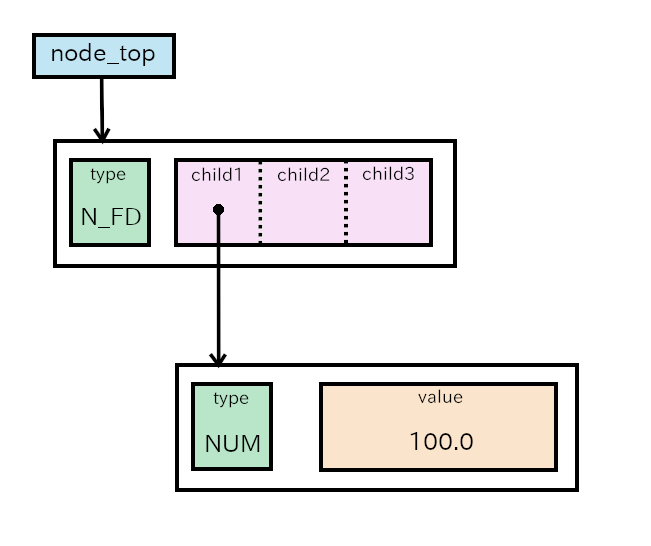
\includegraphics[width=6.51cm,height=5.46cm]{../image/tree.png}
\caption{tree}
\end{figure}

The following is the grammar rule extracted from
\passthrough{\lstinline!turtle.y!}. The rules there are based on the
same idea above. I don't want to explain the whole rules below. Please
look into each line carefully so that you will understand all the rules
and actions.

\begin{lstlisting}
program:
  statement { node_top = $$ = $1; }
| program statement {
        node_top = $$ = tree1 (N_program, $1, $2, NULL);
#ifdef debug
if (node_top == NULL) g_printerr ("program: node_top is NULL.\n"); else g_printerr ("program: node_top is NOT NULL.\n");
#endif
        }
;

statement:
  primary_procedure
| procedure_definition
;

primary_procedure:
  PU    { $$ = tree1 (N_PU, NULL, NULL, NULL); }
| PD    { $$ = tree1 (N_PD, NULL, NULL, NULL); }
| PW expression    { $$ = tree1 (N_PW, $2, NULL, NULL); }
| FD expression    { $$ = tree1 (N_FD, $2, NULL, NULL); }
| TR expression    { $$ = tree1 (N_TR, $2, NULL, NULL); }
| TL expression    { $$ = tree1 (N_TL, $2, NULL, NULL); } /* ver 0.5 */
| BC '(' expression ',' expression ',' expression ')' { $$ = tree1 (N_BC, $3, $5, $7); }
| FC '(' expression ',' expression ',' expression ')' { $$ = tree1 (N_FC, $3, $5, $7); }
 /* assignment */
| ID '=' expression   { $$ = tree1 (N_ASSIGN, tree3 (N_ID, $1), $3, NULL); }
 /* control flow */
| IF '(' expression ')' '{' primary_procedure_list '}' { $$ = tree1 (N_IF, $3, $6, NULL); }
| RT    { $$ = tree1 (N_RT, NULL, NULL, NULL); }
| RS    { $$ = tree1 (N_RS, NULL, NULL, NULL); }
| RP '(' expression ')' '{' primary_procedure_list '}'    { $$ = tree1 (N_RP, $3, $6, NULL); }
 /* user defined procedure call */
| ID '(' ')'  { $$ = tree1 (N_procedure_call, tree3 (N_ID, $1), NULL, NULL); }
| ID '(' argument_list ')'  { $$ = tree1 (N_procedure_call, tree3 (N_ID, $1), $3, NULL); }
;

procedure_definition:
  DP ID '('  ')' '{' primary_procedure_list '}'  {
         $$ = tree1 (N_procedure_definition, tree3 (N_ID, $2), NULL, $6);
        }
| DP ID '(' parameter_list ')' '{' primary_procedure_list '}'  {
         $$ = tree1 (N_procedure_definition, tree3 (N_ID, $2), $4, $7);
        }
;

parameter_list:
  ID { $$ = tree3 (N_ID, $1); }
| parameter_list ',' ID  { $$ = tree1 (N_parameter_list, $1, tree3 (N_ID, $3), NULL); }
;

argument_list:
  expression
| argument_list ',' expression { $$ = tree1 (N_argument_list, $1, $3, NULL); }
;

primary_procedure_list:
  primary_procedure
| primary_procedure_list primary_procedure {
         $$ = tree1 (N_primary_procedure_list, $1, $2, NULL);
        }
;

expression:
  expression '=' expression { $$ = tree1 (N_EQ, $1, $3, NULL); }
| expression '>' expression { $$ = tree1 (N_GT, $1, $3, NULL); }
| expression '<' expression { $$ = tree1 (N_LT, $1, $3, NULL); }
| expression '+' expression { $$ = tree1 (N_ADD, $1, $3, NULL); }
| expression '-' expression { $$ = tree1 (N_SUB, $1, $3, NULL); }
| expression '*' expression { $$ = tree1 (N_MUL, $1, $3, NULL); }
| expression '/' expression { $$ = tree1 (N_DIV, $1, $3, NULL); }
| '-' expression %prec UMINUS { $$ = tree1 (N_UMINUS, $2, NULL, NULL); }
| '(' expression ')' { $$ = $2; }
| ID    { $$ = tree3 (N_ID, $1); }
| NUM   { $$ = tree2 (N_NUM, $1); }
;
\end{lstlisting}

\subsubsection{Epilogue}\label{epilogue}

The epilogue is written in C language and copied to the parser
implementation file. Generally, you can put anything into the epilogue.
In the case of turtle interpreter, the runtime routine and some other
functions are in the epilogue.

\paragraph{Functions to create tree
nodes}\label{functions-to-create-tree-nodes}

There are three functions, \passthrough{\lstinline!tree1!},
\passthrough{\lstinline!tree2!} and \passthrough{\lstinline!tree3!}.

\begin{itemize}
\tightlist
\item
  \passthrough{\lstinline!tree1!} creates a node and sets the node type
  and pointers to its three children (NULL is possible).
\item
  \passthrough{\lstinline!tree2!} creates a node and sets the node type
  and a value (double).
\item
  \passthrough{\lstinline!tree3!} creates a node and sets the node type
  and a pointer to a string.
\end{itemize}

Each function gets memories first and build a node on them. The memories
are inserted to the list. They will be freed when runtime routine
finishes.

The three functions are called in the actions in the rules section.

\begin{lstlisting}[language=C]
/* Dynamically allocated memories are added to the single list. They will be freed in the finalize function. */
GSList *list = NULL;

node_t *
tree1 (int type, node_t *child1, node_t *child2, node_t *child3) {
  node_t *new_node;

  list = g_slist_prepend (list, g_malloc (sizeof (node_t)));
  new_node = (node_t *) list->data;
  new_node->type = type;
  child1(new_node) = child1;
  child2(new_node) = child2;
  child3(new_node) = child3;
  return new_node;
}

node_t *
tree2 (int type, double value) {
  node_t *new_node;

  list = g_slist_prepend (list, g_malloc (sizeof (node_t)));
  new_node = (node_t *) list->data;
  new_node->type = type;
  value(new_node) = value;
  return new_node;
}

node_t *
tree3 (int type, char *name) {
  node_t *new_node;

  list = g_slist_prepend (list, g_malloc (sizeof (node_t)));
  new_node = (node_t *) list->data;
  new_node->type = type;
  name(new_node) = name;
  return new_node;
}
\end{lstlisting}

\paragraph{Symbol table}\label{symbol-table}

Variables and user defined procedures are registered in the symbol
table. This table is a C array. It should be replaced by better
algorithm and data structure, for example hash, in the future version

\begin{itemize}
\tightlist
\item
  Variables are registered with its name and value.
\item
  Procedures are registered with its name and a pointer to the node of
  the procedure.
\end{itemize}

Therefore the table has the following fields.

\begin{itemize}
\tightlist
\item
  type to identify variable or procedure
\item
  name
\item
  value or pointer to a node
\end{itemize}

\begin{lstlisting}[language=C]
#define MAX_TABLE_SIZE 100
enum {
  PROC,
  VAR
};

struct {
  int type;
  char *name;
  union {
    node_t *node;
    double value;
  } object;
} table[MAX_TABLE_SIZE];
int tp;

void
init_table (void) {
  tp = 0;
}
\end{lstlisting}

The function \passthrough{\lstinline!init\_table!} initializes the
table. This must be called before registrations.

There are five functions to access the table,

\begin{itemize}
\tightlist
\item
  \passthrough{\lstinline!proc\_install!} installs a procedure.
\item
  \passthrough{\lstinline!var\_install!} installs a variable.
\item
  \passthrough{\lstinline!proc\_lookup!} looks up a procedure. If the
  procedure is found, it returns a pointer to the node. Otherwise it
  returns NULL.
\item
  \passthrough{\lstinline!var\_lookup!} looks up a variable. If the
  variable is found, it returns TRUE and sets the pointer (argument) to
  point the value. Otherwise it returns FALSE.
\item
  \passthrough{\lstinline!var\_replace!} replaces the value of a
  variable. If the variable hasn't registered yet, it installs the
  variable.
\end{itemize}

\begin{lstlisting}[language=C]
int
tbl_lookup (int type, char *name) {
  int i;

  if (tp == 0)
    return -1;
  for (i=0; i<tp; ++i)
    if (type == table[i].type && strcmp(name, table[i].name) == 0)
      return i;
  return -1;
}

void
tbl_install (int type, char *name, node_t *node, double value) {
  if (tp >= MAX_TABLE_SIZE)
    runtime_error ("Symbol table overflow.\n");
  else if (tbl_lookup (type, name) >= 0)
    runtime_error ("Name %s is already registered.\n", name);
  else {
    table[tp].type = type;
    table[tp].name = name;
    if (type == PROC)
      table[tp++].object.node = node;
    else
      table[tp++].object.value = value;
  }
}

void
proc_install (char *name, node_t *node) {
  tbl_install (PROC, name, node, 0.0);
}

void
var_install (char *name, double value) {
  tbl_install (VAR, name, NULL, value);
}

void
var_replace (char *name, double value) {
  int i;
  if ((i = tbl_lookup (VAR, name)) >= 0)
    table[i].object.value = value;
  else
    var_install (name, value);
}

node_t *
proc_lookup (char *name) {
  int i;
  if ((i = tbl_lookup (PROC, name)) < 0)
    return NULL;
  else
    return table[i].object.node;
}

gboolean
var_lookup (char *name, double *value) {
  int i;
  if ((i = tbl_lookup (VAR, name)) < 0)
    return FALSE;
  else {
    *value = table[i].object.value;
    return TRUE;
  }
}
\end{lstlisting}

\paragraph{Stack for parameters and
arguments}\label{stack-for-parameters-and-arguments}

Stack is a last-in first-out data structure. It is shortened to LIFO.
Turtle uses a stack to keep parameters and arguments. They are like
\passthrough{\lstinline!auto!} class variables in C language. They are
pushed to the stack whenever the procedure is called. LIFO structure is
useful for recursive calls.

Each element of the stack has name and value.

\begin{lstlisting}[language=C]
#define MAX_STACK_SIZE 500
struct {
  char *name;
  double value;
} stack[MAX_STACK_SIZE];
int sp, sp_biggest;

void
init_stack (void) {
  sp = sp_biggest = 0;
}
\end{lstlisting}

\passthrough{\lstinline!sp!} is a stack pointer. It is an index of the
array \passthrough{\lstinline!stack!} and it always points an element of
the array to store the next data. \passthrough{\lstinline!sp\_biggest!}
is the biggest number assigned to \passthrough{\lstinline!sp!}. We can
know the amount of elements used in the array during the runtime. The
purpose of the variable is to find appropriate
\passthrough{\lstinline!MAX\_STACK\_SIZE!}. It will be unnecessary in
the future version if the stack is implemented with better data
structure and memory allocation.

The runtime routine push data to the stack when it executes a node of a
procedure call. (The type of the node is
\passthrough{\lstinline!N\_procedure\_call!}.)

\begin{lstlisting}
dp drawline (angle, distance) { ... ... ... }
drawline (90, 100)
\end{lstlisting}

\begin{itemize}
\tightlist
\item
  The first line defines a procedure \passthrough{\lstinline!drawline!}.
  The runtime routine stores the name \passthrough{\lstinline!drawline!}
  and the node of the procedure to the symbol table.
\item
  The second line calls the procedure. First, it looks for the procedure
  in the symbol table and gets its node. Then it searches the node for
  the parameters and gets \passthrough{\lstinline!angle!} and
  \passthrough{\lstinline!distance!}.
\item
  It pushes (``angle'', 90.0) to the stack.
\item
  It pushes (``distance'', 100.0) to the stack.
\item
  It pushes (NULL, 2.0) to the stack. The number 2.0 is the number of
  parameters (or arguments). It is used when the procedure returns.
\end{itemize}

The following diagram shows the structure of the stack. First,
\passthrough{\lstinline!procedure 1!} is called. The procedure has two
parameters. In the \passthrough{\lstinline!procedure 1!}, another
procedure \passthrough{\lstinline!procedure 2!} is called. It has one
parameter. In the \passthrough{\lstinline!procedure 2!}, another
procedure \passthrough{\lstinline!procedure 3!} is called. It has three
parameters. These three procedures are nested.

Programs push data to a stack from a low address memory to a high
address memory. In the following diagram, the lowest address is at the
top and the highest address is at the bottom. That is the order of the
address. However, ``the top of the stack'' is the last pushed data and
``the bottom of the stack'' is the first pushed data. Therefore, ``the
top of the stack'' is the bottom of the rectangle in the diagram and
``the bottom of the stack'' is the top of the rectangle.

\begin{figure}
\centering
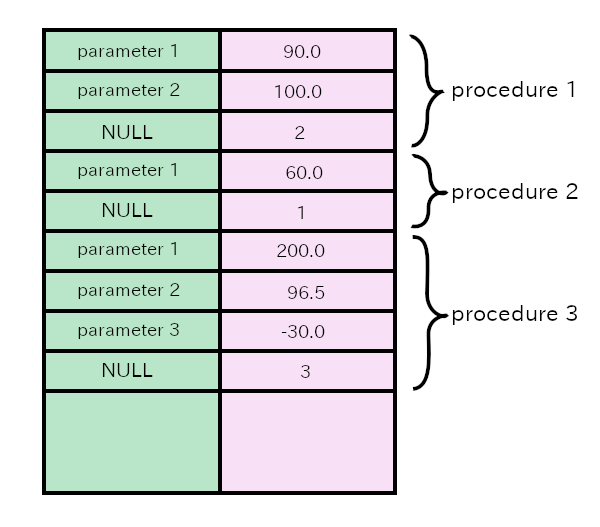
\includegraphics[width=6.64cm,height=8.05cm]{../image/stack.png}
\caption{Stack}
\end{figure}

There are four functions to access the stack.

\begin{itemize}
\tightlist
\item
  \passthrough{\lstinline!stack\_push!} pushes data to the stack.
\item
  \passthrough{\lstinline!stack\_lookup!} searches the stack for the
  variable given its name as an argument. It searches only the
  parameters of the latest procedure. It returns TRUE and sets the
  argument \passthrough{\lstinline!value!} to point the value, if the
  variable has been found. Otherwise it returns FALSE.
\item
  \passthrough{\lstinline!stack\_replace!} replaces the value of the
  variable in the stack. If it succeeds, it returns TRUE. Otherwise
  returns FALSE.
\item
  \passthrough{\lstinline!stack\_return!} throws away the latest
  parameters. The stack pointer goes back to the point before the latest
  procedure call so that it points to parameters of the previous called
  procedure.
\end{itemize}

\begin{lstlisting}[language=C]
void
stack_push (char *name, double value) {
  if (sp >= MAX_STACK_SIZE)
    runtime_error ("Stack overflow.\n");
  else {
    stack[sp].name = name;
    stack[sp++].value = value;
    sp_biggest = sp > sp_biggest ? sp : sp_biggest;
  }
}

int
stack_search (char *name) {
  int depth, i;

  if (sp == 0)
    return -1;
  depth = (int) stack[sp-1].value;
  if (depth + 1 > sp) /* something strange */
    runtime_error ("Stack error.\n");
  for (i=0; i<depth; ++i)
    if (strcmp(name, stack[sp-(i+2)].name) == 0) {
      return sp-(i+2);
    }
  return -1;
}

gboolean
stack_lookup (char *name, double *value) {
  int i;

  if ((i = stack_search (name)) < 0)
    return FALSE;
  else {
    *value = stack[i].value;
    return TRUE;
  }
}

gboolean
stack_replace (char *name, double value) {
  int i;

  if ((i = stack_search (name)) < 0)
    return FALSE;
  else {
    stack[i].value = value;
    return TRUE;
  }
}

void
stack_return(void) {
  int depth;

  if (sp <= 0)
    return;
  depth = (int) stack[sp-1].value;
  if (depth + 1 > sp) /* something strange */
    runtime_error ("Stack error.\n");
  sp -= depth + 1;
}
\end{lstlisting}

\paragraph{Surface and cairo}\label{surface-and-cairo}

A global variable \passthrough{\lstinline!surface!} is shared by
\passthrough{\lstinline!turtleapplication.c!} and
\passthrough{\lstinline!turtle.y!}. It is initialized in
\passthrough{\lstinline!turtleapplication.c!}.

The runtime routine has its own cairo context. This is different from
the cairo in the GtkDrawingArea instance. The runtime routine draws a
shape on the \passthrough{\lstinline!surface!} with the cairo context.
After runtime routine returns to \passthrough{\lstinline!run\_cb!},
\passthrough{\lstinline!run\_cb!} adds the GtkDrawingArea widget to the
queue to redraw. When the widget is redraw,the drawing function
\passthrough{\lstinline!draw\_func!} is called. It copies the
\passthrough{\lstinline!surface!} to the surface in the GtkDrawingArea
object.

\passthrough{\lstinline!turtle.y!} has two functions
\passthrough{\lstinline!init\_cairo!} and
\passthrough{\lstinline!destroy\_cairo!}.

\begin{itemize}
\tightlist
\item
  \passthrough{\lstinline!init\_cairo!} initializes static variables and
  cairo context. The variables keep pen status (up or down), direction,
  initial location, line width and color. The size of the
  \passthrough{\lstinline!surface!} changes according to the size of the
  window. Whenever a user drags and resizes the window, the
  \passthrough{\lstinline!surface!} is also resized.
  \passthrough{\lstinline!init\_cairo!} gets the size first and sets the
  initial location of the turtle (center of the surface) and the
  transformation matrix.
\item
  \passthrough{\lstinline!destroy\_cairo!} just destroys the cairo
  context.
\end{itemize}

Turtle has its own coordinate. The origin is at the center of the
surface, and positive direction of x and y axes are right and up
respectively. But surfaces have its own coordinate. Its origin is at the
top-left corner of the surface and positive direction of x and y are
right and down respectively. A plane with the turtle's coordinate is
called user space, which is the same as cairo's user space. A plane with
the surface's coordinate is called device space.

Cairo provides a transformation which is an affine transformation. It
transforms a user-space coordinate (x, y) into a device-space coordinate
(z, w).

\begin{figure}
\centering
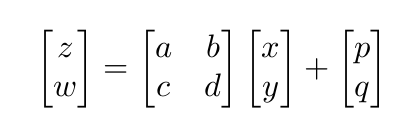
\includegraphics[width=6.3cm,height=2.04cm]{../image/transformation.png}
\caption{transformation}
\end{figure}

The function \passthrough{\lstinline!init\_cairo!} gets the width and
height of the \passthrough{\lstinline!surface!} (See the program below).

\begin{itemize}
\tightlist
\item
  The center of the surface is (0,0) with regard to the user-space
  coordinate and (width/2, height/2) with regard to the device-space
  coordinate.
\item
  The positive direction of x axis in the two spaces are the same. So,
  (1,0) is transformed into (1+width/2,height/2).
\item
  The positive direction of y axis in the two spaces are opposite. So,
  (0,1) is transformed into (width/2,-1+height/2).
\end{itemize}

You can determine a, b, c, d, p and q by substituting the numbers above
for x, y, z and w in the equation above. The solution of the
simultaneous equations is:

\begin{lstlisting}
a = 1, b = 0, c = 0, d = -1, p = width/2, q = height/2
\end{lstlisting}

Cairo provides a structure \passthrough{\lstinline!cairo\_matrix\_t!}.
The function \passthrough{\lstinline!init\_cairo!} uses it and sets the
cairo transformation (See the program below). Once the matrix is set,
the transformation always performs whenever
\passthrough{\lstinline!cairo\_stroke!} function is invoked.

\begin{lstlisting}[language=C]
/* status of the surface */
static gboolean pen = TRUE;
static double angle = 90.0; /* angle starts from x axis and measured counterclockwise */
                   /* Initially facing to the north */
static double cur_x = 0.0;
static double cur_y = 0.0;
static double line_width = 2.0;

struct color {
  double red;
  double green;
  double blue;
};
static struct color bc = {0.95, 0.95, 0.95}; /* white */
static struct color fc = {0.0, 0.0, 0.0}; /* black */

/* cairo */
static cairo_t *cr;
gboolean
init_cairo (void) {
  int width, height;
  cairo_matrix_t matrix;

  pen = TRUE;
  angle = 90.0;
  cur_x = 0.0;
  cur_y = 0.0;
  line_width = 2.0;
  bc.red = 0.95; bc.green = 0.95; bc.blue = 0.95;
  fc.red = 0.0; fc.green = 0.0; fc.blue = 0.0;

  if (surface) {
    width = cairo_image_surface_get_width (surface);
    height = cairo_image_surface_get_height (surface);
    matrix.xx = 1.0; matrix.xy = 0.0; matrix.x0 = (double) width / 2.0;
    matrix.yx = 0.0; matrix.yy = -1.0; matrix.y0 = (double) height / 2.0;

    cr = cairo_create (surface);
    cairo_transform (cr, &matrix);
    cairo_set_source_rgb (cr, bc.red, bc.green, bc.blue);
    cairo_paint (cr);
    cairo_set_source_rgb (cr, fc.red, fc.green, fc.blue);
    cairo_move_to (cr, cur_x, cur_y);
    return TRUE;
  } else
    return FALSE;
}

void
destroy_cairo () {
  cairo_destroy (cr);
}
\end{lstlisting}

\paragraph{Eval function}\label{eval-function}

A function \passthrough{\lstinline!eval!} evaluates an expression and
returns the value of the expression. It calls itself recursively. For
example, if the node is \passthrough{\lstinline!N\_ADD!}, then:

\begin{enumerate}
\def\labelenumi{\arabic{enumi}.}
\tightlist
\item
  Calls eval(child1(node)) and gets the value1.
\item
  Calls eval(child2(node)) and gets the value2.
\item
  Returns value1+value2.
\end{enumerate}

This is performed by a macro \passthrough{\lstinline!calc!} defined in
the sixth line in the following program.

\begin{lstlisting}[language=C]
double
eval (node_t *node) {
double value = 0.0;
  if (node == NULL)
    runtime_error ("No expression to evaluate.\n");
#define calc(op) eval (child1(node)) op eval (child2(node))
  switch (node->type) {
    case N_EQ:
      value = (double) calc(==);
      break;
    case N_GT:
      value = (double) calc(>);
      break;
    case N_LT:
      value = (double) calc(<);
      break;
    case N_ADD:
      value = calc(+);
      break;
    case N_SUB:
      value = calc(-);
      break;
    case N_MUL:
      value = calc(*);
      break;
    case N_DIV:
      if (eval (child2(node)) == 0.0)
        runtime_error ("Division by zerp.\n");
      else
        value = calc(/);
      break;
    case N_UMINUS:
      value = -(eval (child1(node)));
      break;
    case N_ID:
      if (! (stack_lookup (name(node), &value)) && ! var_lookup (name(node), &value) )
        runtime_error ("Variable %s not defined.\n", name(node));
      break;
    case N_NUM:
      value = value(node);
      break;
    default:
      runtime_error ("Illegal expression.\n");
  }
  return value;
}
\end{lstlisting}

\paragraph{Execute function}\label{execute-function}

Primary procedures and procedure definitions are analyzed and executed
by the function \passthrough{\lstinline!execute!}. It doesn't return any
values. It calls itself recursively. The process of
\passthrough{\lstinline!N\_RT!} and
\passthrough{\lstinline!N\_procedure\_call!} is complicated. It will
explained after the following program. Other parts are not so difficult.
Read the program below carefully so that you will understand the
process.

\begin{lstlisting}[language=C]
/* procedure - return status */
static int proc_level = 0;
static int ret_level = 0;

void
execute (node_t *node) {
  double d, x, y;
  char *name;
  int n, i;

  if (node == NULL)
    runtime_error ("Node is NULL.\n");
  if (proc_level > ret_level)
    return;
  switch (node->type) {
    case N_program:
      execute (child1(node));
      execute (child2(node));
      break;
    case N_PU:
      pen = FALSE;
      break;
    case N_PD:
      pen = TRUE;
      break;
    case N_PW:
      line_width = eval (child1(node)); /* line width */
      break;
    case N_FD:
      d = eval (child1(node)); /* distance */
      x = d * cos (angle*M_PI/180);
      y = d * sin (angle*M_PI/180);
      /* initialize the current point = start point of the line */
      cairo_move_to (cr, cur_x, cur_y);
      cur_x += x;
      cur_y += y;
      cairo_set_line_width (cr, line_width);
      cairo_set_source_rgb (cr, fc.red, fc.green, fc.blue);
      if (pen)
        cairo_line_to (cr, cur_x, cur_y);
      else
        cairo_move_to (cr, cur_x, cur_y);
      cairo_stroke (cr);
      break;
    case N_TR:
      angle -= eval (child1(node));
      for (; angle < 0; angle += 360.0);
      for (; angle>360; angle -= 360.0);
      break;
    case N_BC:
      bc.red = eval (child1(node));
      bc.green = eval (child2(node));
      bc.blue = eval (child3(node));
#define fixcolor(c)  c = c < 0 ? 0 : (c > 1 ? 1 : c)
      fixcolor (bc.red);
      fixcolor (bc.green);
      fixcolor (bc.blue);
      /* clear the shapes and set the background color */
      cairo_set_source_rgb (cr, bc.red, bc.green, bc.blue);
      cairo_paint (cr);
      break;
    case N_FC:
      fc.red = eval (child1(node));
      fc.green = eval (child2(node));
      fc.blue = eval (child3(node));
      fixcolor (fc.red);
      fixcolor (fc.green);
      fixcolor (fc.blue);
      break;
    case N_ASSIGN:
      name = name(child1(node));
      d = eval (child2(node));
      if (! stack_replace (name, d)) /* First, tries to replace the value in the stack (parameter).*/
        var_replace (name, d); /* If the above fails, tries to replace the value in the table. If the variable isn't in the table, installs it, */
      break;
    case N_IF:
      if (eval (child1(node)))
        execute (child2(node));
      break;
    case N_RT:
      ret_level--;
      break;
    case N_RS:
      pen = TRUE;
      angle = 90.0;
      cur_x = 0.0;
      cur_y = 0.0;
      line_width = 2.0;
      fc.red = 0.0; fc.green = 0.0; fc.blue = 0.0;
      /* To change background color, use bc. */
      break;
    case N_procedure_call:
      name = name(child1(node));
node_t *proc = proc_lookup (name);
      if (! proc)
        runtime_error ("Procedure %s not defined.\n", name);
      if (strcmp (name, name(child1(proc))) != 0)
        runtime_error ("Unexpected error. Procedure %s is called, but invoked procedure is %s.\n", name, name(child1(proc)));
/* make tuples (parameter (name), argument (value)) and push them to the stack */
node_t *param_list;
node_t *arg_list;
      param_list = child2(proc);
      arg_list = child2(node);
      if (param_list == NULL) {
        if (arg_list == NULL) {
          stack_push (NULL, 0.0); /* number of argument == 0 */
        } else
          runtime_error ("Procedure %s has different number of argument and parameter.\n", name);
      }else {
/* Don't change the stack until finish evaluating the arguments. */
#define TEMP_STACK_SIZE 20
        char *temp_param[TEMP_STACK_SIZE];
        double temp_arg[TEMP_STACK_SIZE];
        n = 0;
        for (; param_list->type == N_parameter_list; param_list = child1(param_list)) {
          if (arg_list->type != N_argument_list)
            runtime_error ("Procedure %s has different number of argument and parameter.\n", name);
          if (n >= TEMP_STACK_SIZE)
            runtime_error ("Too many parameters. the number must be %d or less.\n", TEMP_STACK_SIZE);
          temp_param[n] = name(child2(param_list));
          temp_arg[n] = eval (child2(arg_list));
          arg_list = child1(arg_list);
          ++n;
        }
        if (param_list->type == N_ID && arg_list -> type != N_argument_list) {
          temp_param[n] = name(param_list);
          temp_arg[n] = eval (arg_list);
          if (++n >= TEMP_STACK_SIZE)
            runtime_error ("Too many parameters. the number must be %d or less.\n", TEMP_STACK_SIZE);
          temp_param[n] = NULL;
          temp_arg[n] = (double) n;
          ++n;
        } else
          runtime_error ("Unexpected error.\n");
        for (i = 0; i < n; ++i)
          stack_push (temp_param[i], temp_arg[i]);
      }
      ret_level = ++proc_level;
      execute (child3(proc));
      ret_level = --proc_level;
      stack_return ();
      break;
    case N_procedure_definition:
      name = name(child1(node));
      proc_install (name, node);
      break;
    case N_primary_procedure_list:
      execute (child1(node));
      execute (child2(node));
      break;
    default:
      runtime_error ("Unknown statement.\n");
  }
}
\end{lstlisting}

A node \passthrough{\lstinline!N\_procedure\_call!} is created by the
parser when it has found a user defined procedure call. The procedure
has been defined in the prior statement. Suppose the parser reads the
following example code.

\begin{lstlisting}
dp drawline (angle, distance) {
  tr angle
  fd distance
}
drawline (90, 100)
drawline (90, 100)
drawline (90, 100)
drawline (90, 100)
\end{lstlisting}

This example draws a square.

When The parser reads the lines from one to four, it creates nodes like
this:

\begin{figure}
\centering
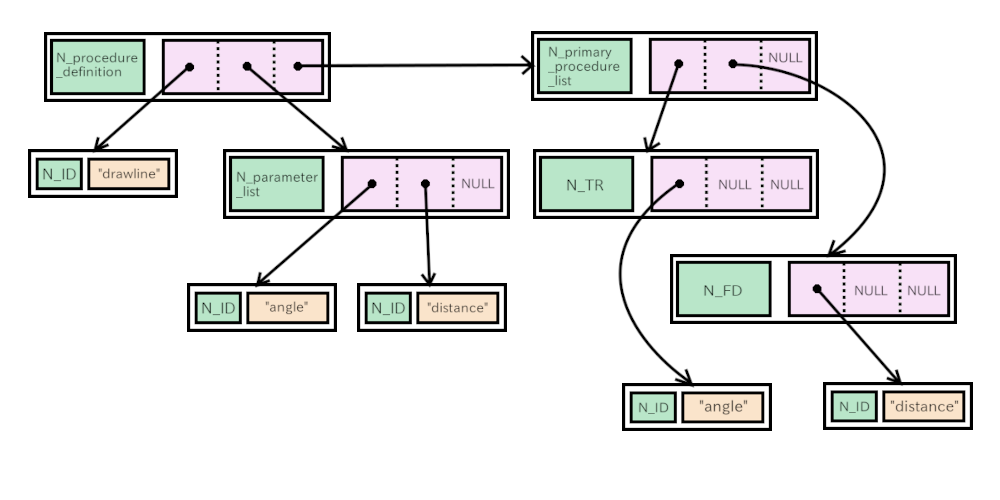
\includegraphics[width=10cm,height=6cm]{../image/tree2.png}
\caption{Nodes of drawline}
\end{figure}

Runtime routine just stores the procedure to the symbol table with its
name and node.

\begin{figure}
\centering
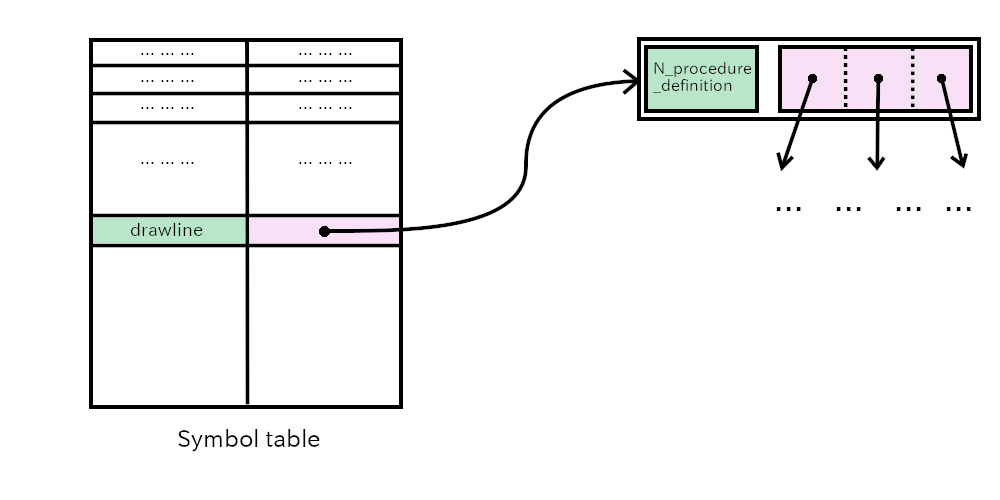
\includegraphics[width=10cm,height=5cm]{../image/table.png}
\caption{Symbol table}
\end{figure}

When the parser reads the fifth line in the example, it creates nodes
like this:

\begin{figure}
\centering
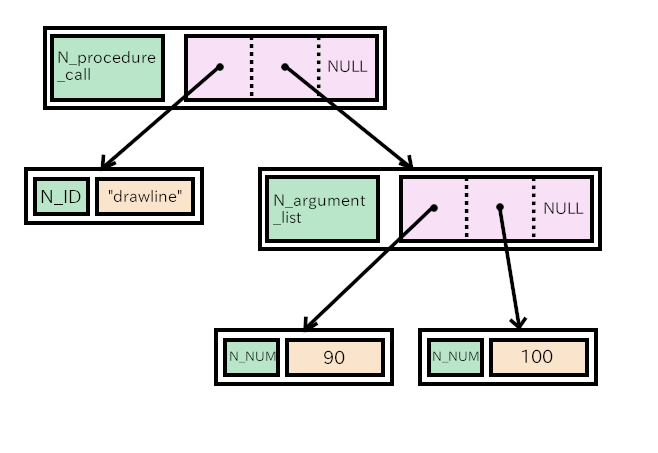
\includegraphics[width=10cm,height=5cm]{../image/proc_call.png}
\caption{Nodes of procedure call}
\end{figure}

When the runtime routine meets
\passthrough{\lstinline!N\_procedure\_call!} node, it behaves like this:

\begin{enumerate}
\def\labelenumi{\arabic{enumi}.}
\tightlist
\item
  Searches the symbol table for the procedure with the name.
\item
  Gets pointers to the node to parameters and the node to the body.
\item
  Creates a temporary stack. Makes a tuple of each parameter name and
  argument value. Pushes the tuples into the stack, and (NULL, number of
  parameters) finally. If no error occurs, copies them from the
  temporary stack to the parameter stack.
\item
  Increases \passthrough{\lstinline!prc\_level!} by one. Sets
  \passthrough{\lstinline!ret\_level!} to the same value as
  \passthrough{\lstinline!proc\_level!}.
  \passthrough{\lstinline!proc\_level!} is zero when runtime routine
  runs on the main routine. If it goes into a procedure,
  \passthrough{\lstinline!proc\_level!} increases by one. Therefore,
  \passthrough{\lstinline!proc\_level!} is the depth of the procedure
  call. \passthrough{\lstinline!ret\_level!} is the level to return. If
  it is the same as \passthrough{\lstinline!proc\_level!}, runtime
  routine executes commands in order of the commands in the procedure.
  If it is smaller than \passthrough{\lstinline!proc\_level!}, runtime
  routine doesn't execute commands until it becomes the same level as
  \passthrough{\lstinline!proc\_level!}.
  \passthrough{\lstinline!ret\_level!} is used to return the procedure.
\item
  Executes the node of the body of the procedure.
\item
  Decreases \passthrough{\lstinline!proc\_level!} by one. Sets
  \passthrough{\lstinline!ret\_level!} to the same value as
  \passthrough{\lstinline!proc\_level!}. Calls
  \passthrough{\lstinline!stack\_return!}.
\end{enumerate}

When the runtime routine meets \passthrough{\lstinline!N\_RT!} node, it
decreases \passthrough{\lstinline!ret\_level!} by one so that the
following commands in the procedure are ignored by the runtime routine.

\paragraph{Runtime entry and error
functions}\label{runtime-entry-and-error-functions}

A function \passthrough{\lstinline!run!} is the entry of the runtime
routine. A function \passthrough{\lstinline!runtime\_error!} reports an
error occurred during the runtime routine runs. (Errors which occur
during the parsing are called syntax error and reported by
\passthrough{\lstinline!yyerror!}.) After
\passthrough{\lstinline!runtime\_error!} reports an error, it stops the
command execution and goes back to \passthrough{\lstinline!run!} to
exit.

Setjmp and longjmp functions are used. They are declared in
\passthrough{\lstinline!<setjmp.h>!}.
\passthrough{\lstinline!setjmp (buf)!} saves state information in
\passthrough{\lstinline!buf!} and returns zero.
\passthrough{\lstinline!longjmp(buf, 1)!} restores the state information
from \passthrough{\lstinline!buf!} and returns
\passthrough{\lstinline!1!} (the second argument). Because the
information is the status at the time \passthrough{\lstinline!setjmp!}
is called, so longjmp resumes the execution at the next of setjmp
function call. In the following program, longjmp resumes at the
assignment to the variable \passthrough{\lstinline!i!}. When setjmp is
called, 0 is assigned to \passthrough{\lstinline!i!} and
\passthrough{\lstinline!execute(node\_top)!} is called. On the other
hand, when longjmp is called, 1 is assigned to
\passthrough{\lstinline!i!} and
\passthrough{\lstinline!execute(node\_top)!} is not called..

\passthrough{\lstinline!g\_slist\_free\_full!} frees all the allocated
memories.

\begin{lstlisting}[language=C]
static jmp_buf buf;

void
run (void) {
  int i;

  if (! init_cairo()) {
    g_print ("Cairo not initialized.\n");
    return;
  }
  init_table();
  init_stack();
  ret_level = proc_level = 1;
  i = setjmp (buf);
  if (i == 0)
    execute(node_top);
  /* else ... get here by calling longjmp */
  destroy_cairo ();
  g_slist_free_full (g_steal_pointer (&list), g_free);
}

/* format supports only %s, %f and %d */
static void
runtime_error (char *format, ...) {
  va_list args;
  char *f;
  char b[3];
  char *s;
  double v;
  int i;

  va_start (args, format);
  for (f = format; *f; f++) {
    if (*f != '%') {
      b[0] = *f;
      b[1] = '\0';
      g_print ("%s", b);
      continue;
    }
    switch (*++f) {
      case 's':
        s = va_arg(args, char *);
        g_print ("%s", s);
        break;
      case 'f':
        v = va_arg(args, double);
        g_print("%f", v);
        break;
      case 'd':
        i = va_arg(args, int);
        g_print("%d", i);
        break;
      default:
        b[0] = '%';
        b[1] = *f;
        b[2] = '\0';
        g_print ("%s", b);
        break;
    }
  }
  va_end (args);

  longjmp (buf, 1);
}
\end{lstlisting}

A function \passthrough{\lstinline!runtime\_error!} has a
variable-length argument list.

\begin{lstlisting}[language=C]
void runtime_error (char *format, ...)
\end{lstlisting}

This is implemented with \passthrough{\lstinline!<stdarg.h>!} header
file. The \passthrough{\lstinline!va\_list!} type variable
\passthrough{\lstinline!args!} will refer to each argument in turn. A
function \passthrough{\lstinline!va\_start!} initializes
\passthrough{\lstinline!args!}. A function
\passthrough{\lstinline!va\_arg!} returns an argument and moves the
reference of \passthrough{\lstinline!args!} to the next. A function
\passthrough{\lstinline!va\_end!} cleans up everything necessary at the
end.

The function \passthrough{\lstinline!runtime\_error!} has a similar
format of printf standard function. But its format has only
\passthrough{\lstinline!\%s!}, \passthrough{\lstinline!\%f!} and
\passthrough{\lstinline!\%d!}.

The functions declared in \passthrough{\lstinline!<setjmp.h>!} and
\passthrough{\lstinline!<stdarg.h>!} are explained in the very famous
book ``The C programming language'' written by Brian Kernighan and
Dennis Ritchie. I referred to the book to write the program above.

The program \passthrough{\lstinline!turtle!} is unsophisticated and
unpolished. If you want to make your own language, you need to know more
and more. I don't know any good textbook about compilers and
interpreters. If you know a good book, please let me know.

However, the following information is very useful (but old).

\begin{itemize}
\tightlist
\item
  Bison documentation
\item
  Flex documentation
\item
  Software tools written by Brian W. Kernighan \& P. J. Plauger (1976)
\item
  Unix programming environment written by Brian W. Kernighan and Rob
  Pike (1984)
\item
  Source code of a language, for example, ruby.
\end{itemize}

Lately, lots of source codes are in the internet. Maybe reading source
codes is the most useful for programmers.

  \section{Drag and drop}\label{drag-and-drop}

\subsection{What's drag and drop?}\label{whats-drag-and-drop}

Drag and drop is also written as ``Drag-and-Drop'', or ``DND'' in short.
DND is like ``copy and paste'' or ``cut and paste''. If a user drags a
UI element, which is a widget, selected part or something, data is
transferred from the source to the destination.

You probably have experience that you moved a file with DND.

\begin{figure}
\centering
\includegraphics[width=4.6cm,height=3cm]{../image/dnd.png}
\caption{DND on the GUI file manager}
\end{figure}

When the DND starts, the file \passthrough{\lstinline!sample\_file.txt!}
is given to the system. When the DND ends, the system gives
\passthrough{\lstinline!sample\_file.txt!} to the directory
\passthrough{\lstinline!sample\_folder!} in the file manager. Therefore,
it is like ``cut and paste''. The actual behavior may be different from
the explanation here, but the concept is similar.

\subsection{Example for DND}\label{example-for-dnd}

This tutorial provides a simple example in the
\passthrough{\lstinline!src/dnd!} directory. It has three labels for the
source and one label for the destination. The source labels have
``red'', ``green'' or ``blue'' labels. If a user drags the label to the
destination label, the font color will be changed.

\begin{figure}
\centering
\includegraphics[width=13.5cm,height=5.2cm]{../image/dnd_canvas.png}
\caption{DND example}
\end{figure}

\subsection{UI file}\label{ui-file}

The widgets are defined in the XML file
\passthrough{\lstinline!dnd.ui!}.

\begin{lstlisting}[language=XML, numbers=left]
<?xml version="1.0" encoding="UTF-8"?>
<interface>
  <object class="GtkApplicationWindow" id="win">
    <property name="default-width">800</property>
    <property name="default-height">600</property>
    <property name="resizable">FALSE</property>
    <property name="title">Drag and Drop</property>
    <child>
      <object class="GtkBox">
        <property name="hexpand">TRUE</property>
        <property name="vexpand">TRUE</property>
        <property name="orientation">GTK_ORIENTATION_VERTICAL</property>
        <property name="spacing">5</property>
        <child>
          <object class="GtkBox">
            <property name="orientation">GTK_ORIENTATION_HORIZONTAL</property>
            <property name="homogeneous">TRUE</property>
            <child>
              <object class="GtkLabel" id="red">
                <property name="label">RED</property>
                <property name="justify">GTK_JUSTIFY_CENTER</property>
                <property name="name">red</property>
              </object>
            </child>
            <child>
              <object class="GtkLabel" id="green">
                <property name="label">GREEN</property>
                <property name="justify">GTK_JUSTIFY_CENTER</property>
                <property name="name">green</property>
              </object>
            </child>
            <child>
              <object class="GtkLabel" id="blue">
                <property name="label">BLUE</property>
                <property name="justify">GTK_JUSTIFY_CENTER</property>
                <property name="name">blue</property>
              </object>
            </child>
          </object>
        </child>
        <child>
          <object class="GtkLabel" id="canvas">
            <property name="label">CANVAS</property>
            <property name="justify">GTK_JUSTIFY_CENTER</property>
            <property name="name">canvas</property>
            <property name="hexpand">TRUE</property>
            <property name="vexpand">TRUE</property>
          </object>
        </child>
      </object>
    </child>
  </object>
</interface>
\end{lstlisting}

It is converted to a resource file by
\passthrough{\lstinline!glib-compile-resources!}. The compiler uses an
XML file \passthrough{\lstinline!dnd.gresource.xml!}.

\begin{lstlisting}[language=XML, numbers=left]
<?xml version="1.0" encoding="UTF-8"?>
<gresources>
  <gresource prefix="/com/github/ToshioCP/dnd">
    <file>dnd.ui</file>
  </gresource>
</gresources>
\end{lstlisting}

\subsection{C file dnd.c}\label{c-file-dnd.c}

The C file \passthrough{\lstinline!dnd.c!} isn't a big file. The number
of the lines is less than a hundred. A GtkApplication object is created
in the function \passthrough{\lstinline!main!}.

\begin{lstlisting}[language=C, numbers=left]
int
main (int argc, char **argv) {
  GtkApplication *app;
  int stat;

  app = gtk_application_new (APPLICATION_ID, G_APPLICATION_DEFAULT_FLAGS);
  g_signal_connect (app, "startup", G_CALLBACK (app_startup), NULL);
  g_signal_connect (app, "activate", G_CALLBACK (app_activate), NULL);
  stat =g_application_run (G_APPLICATION (app), argc, argv);
  g_object_unref (app);
  return stat;
}
\end{lstlisting}

The application ID is defined as:

\begin{lstlisting}[language=C]
#define APPLICATION_ID "com.github.ToshioCP.dnd"
\end{lstlisting}

\subsubsection{Startup signal handler}\label{startup-signal-handler}

Most of the work is done in the ``startup'' signal handler.

Two objects GtkDragSource and GtkDropTarget is used for DND
implementation.

\begin{itemize}
\tightlist
\item
  Drag source: A drag source (GtkDragSource instance) is an event
  controller. It initiates a DND operation when the user clicks and
  drags the widget. If a data, in the form of GdkContentProvider, is set
  in advance, it gives the data to the system at the beginning of the
  drag.
\item
  Drop target: A drop target (GtkDropTarget) is also an event
  controller. You can get the data in the GtkDropTarget::drop signal
  handler.
\end{itemize}

The example below uses these objects in a very simple way. You can use
number of features that the two objects have. See the following links
for more information.

\begin{itemize}
\tightlist
\item
  \href{https://docs.gtk.org/gtk4/drag-and-drop.html}{Drag-and-Drop in
  GTK}
\item
  \href{https://docs.gtk.org/gtk4/class.DragSource.html}{GtkDragSource}
\item
  \href{https://docs.gtk.org/gtk4/class.DropTarget.html}{GtkDropTarget}
\end{itemize}

\begin{lstlisting}[language=C, numbers=left]
static void
app_startup (GApplication *application) {
  GtkApplication *app = GTK_APPLICATION (application);
  GtkBuilder *build;
  GtkWindow *win;
  GtkLabel *src_labels[3];
  int i;
  GtkLabel *canvas;
  GtkDragSource *src;
  GdkContentProvider* content;
  GtkDropTarget *tgt;
  GdkDisplay *display;
  char *s;

  build = gtk_builder_new_from_resource ("/com/github/ToshioCP/dnd/dnd.ui");
  win = GTK_WINDOW (gtk_builder_get_object (build, "win"));
  src_labels[0] = GTK_LABEL (gtk_builder_get_object (build, "red"));
  src_labels[1] = GTK_LABEL (gtk_builder_get_object (build, "green"));
  src_labels[2] = GTK_LABEL (gtk_builder_get_object (build, "blue"));
  canvas = GTK_LABEL (gtk_builder_get_object (build, "canvas"));
  gtk_window_set_application (win, app);
  g_object_unref (build);

  for (i=0; i<3; ++i) {
    src = gtk_drag_source_new ();
    content = gdk_content_provider_new_typed (G_TYPE_STRING, gtk_widget_get_name (GTK_WIDGET (src_labels[i])));
    gtk_drag_source_set_content (src, content);
    g_object_unref (content);
    gtk_widget_add_controller (GTK_WIDGET (src_labels[i]), GTK_EVENT_CONTROLLER (src)); // The ownership of src is taken by the instance.
  }

  tgt = gtk_drop_target_new (G_TYPE_STRING, GDK_ACTION_COPY);
  g_signal_connect (tgt, "drop", G_CALLBACK (drop_cb), NULL);
  gtk_widget_add_controller (GTK_WIDGET (canvas), GTK_EVENT_CONTROLLER (tgt)); // The ownership of tgt is taken by the instance.

  provider = gtk_css_provider_new ();
  s = g_strdup_printf (format, "black");
  gtk_css_provider_load_from_data (provider, s, -1);
  g_free (s);
  display = gdk_display_get_default ();
  gtk_style_context_add_provider_for_display (display, GTK_STYLE_PROVIDER (provider),
                                              GTK_STYLE_PROVIDER_PRIORITY_APPLICATION);
  g_object_unref (provider); // The provider is still alive because the display owns it.
}
\end{lstlisting}

\begin{itemize}
\tightlist
\item
  15-22: Builds the widgets. The array
  \passthrough{\lstinline!source\_labels[]!} points the source labels
  red, green and blue in the ui file. The variable
  \passthrough{\lstinline!canvas!} points the destination label.
\item
  24-30: Sets the DND source widgets. The for-loop carries out through
  the array \passthrough{\lstinline!src\_labels[]!} each of which points
  the source widget, red, green or blue label.
\item
  25: Creates a new GtkDragSource instance.
\item
  26: Creates a new GdkContentProvider instance with the string ``red'',
  ``green'' or ``blue. They are the name of the widgets. These strings
  are the data to transfer through the DND operation.
\item
  27: Sets the content of the drag source to the GdkContentProvider
  instance above.
\item
  28: Content is useless so it is destroyed.
\item
  29: Add the event controller, which is actually the drag source, to
  the widget. If a DND operation starts on the widget, the corresponding
  drag source works and the data is given to the system.
\item
  32-34: Sets the DND drop target.
\item
  32: Creates a new GtkDropTarget instance. The first parameter is the
  GType of the data. The second parameter is a GdkDragAction enumerate
  constant. The arguments here are string type and the constant for
  copy.
\item
  33: Connects the ``drop'' signal and the handler
  \passthrough{\lstinline!drop\_cb!}.
\item
  34: Add the event controller, which is actually the drop target, to
  the widget.
\item
  36-43: Sets CSS.
\item
  37: A varable \passthrough{\lstinline!format!} is static and defined
  at the top of the program. Static variables are shown below.
\end{itemize}

\begin{lstlisting}[language=C]
static GtkCssProvider *provider = NULL;
static const char *format = "label {padding: 20px;} label#red {background: red;} "
  "label#green {background: green;} label#blue {background: blue;} "
  "label#canvas {color: %s; font-weight: bold; font-size: 72pt;}";
\end{lstlisting}

\subsubsection{Activate signal handler}\label{activate-signal-handler}

\begin{lstlisting}[language=C, numbers=left]
static void
app_activate (GApplication *application) {
  GtkApplication *app = GTK_APPLICATION (application);
  GtkWindow *win;

  win = gtk_application_get_active_window (app);
  gtk_window_present (win);
}
\end{lstlisting}

This handler just shows the window.

\subsubsection{Drop signal handler}\label{drop-signal-handler}

\begin{lstlisting}[language=C, numbers=left]
static gboolean
drop_cb (GtkDropTarget* self, const GValue* value, gdouble x, gdouble y, gpointer user_data) {
  char *s;

  s = g_strdup_printf (format, g_value_get_string (value));
  gtk_css_provider_load_from_data (provider, s, -1);
  g_free (s);
  return TRUE;
}
\end{lstlisting}

The ``drop'' signal handler has five parameters.

\begin{itemize}
\tightlist
\item
  GtkDropTarget instance on which the signal has been emitted.
\item
  GValue that holds the data from the source.
\item
  The arguments \passthrough{\lstinline!x!} and
  \passthrough{\lstinline!y!} are the coordinate of the mouse when
  released.
\item
  User data was set when the signal and handler was connected.
\end{itemize}

The string from the GValue is ``red'', ``green'' or ``blue''. It
replaces ``\%s'' in the variable \passthrough{\lstinline!format!}. That
means the font color of the label \passthrough{\lstinline!canvas!} will
turn to the color.

\subsection{Meson.build}\label{meson.build}

The file \passthrough{\lstinline!meson.build!} controls the building
process.

\begin{lstlisting}[numbers=left]
project('dnd', 'c')

gtkdep = dependency('gtk4')

gnome = import('gnome')
resources = gnome.compile_resources('resources','dnd.gresource.xml')

executable(meson.project_name(), 'dnd.c', resources, dependencies: gtkdep, export_dynamic: true, install: false)
\end{lstlisting}

You can build it from the command line.

\begin{lstlisting}
$ cd src/dnd
$ meson setup _build
$ ninja -C _build
$ _build/dnd
\end{lstlisting}

The source files are under the directory
\passthrough{\lstinline!src/dnd!} of the
\href{https://github.com/ToshioCP/Gtk4-tutorial}{repository}. Download
it and see the directory.

  \section{GtkListView}\label{gtklistview}

GTK 4 has added new list objects GtkListView, GtkGridView and
GtkColumnView. The new feature is described in
\href{https://docs.gtk.org/gtk4/section-list-widget.html}{Gtk API
Reference -- List Widget Overview}.

GTK 4 has other means to implement lists. They are GtkListBox and
GtkTreeView which are took over from GTK 3. There's an article in
\href{https://blog.gtk.org/2020/06/07/scalable-lists-in-gtk-4/}{Gtk
Development blog} about list widgets by Matthias Clasen. He described
why GtkListView are developed to replace GtkTreeView. GtkTreeView is
deprecated since version 4.10.

GtkListView, GtkGridView, GtkColumnView and related objects are
described in Section 29 to 33.

\subsection{Outline}\label{outline}

A list is a sequential data structure. For example, an ordered string
sequence ``one'', ``two'', ``three'', ``four'' is a list. Each element
is called item. A list is like an array, but in many cases it is
implemented with pointers which point to the next items of the list. And
it has a start point. So, each item can be referred by the index of the
item (first item, second item, \ldots, nth item, \ldots). There are two
cases. The one is the index starts from one (one-based) and the other is
from zero (zero-based).

Gio provides GListModel interface. It is a zero-based list and its items
are the same type of GObject descendants, or objects that implement the
same interface. An object implements GListModel is not a widget. So, the
list is not displayed on the screen directly. There's another object
GtkListView which is a widget to display the list. The items in the list
need to be connected to the items in GtkListView. GtkListItemFactory
instance maps items in the list to GtkListView.

\begin{figure}
\centering
\includegraphics[width=10cm,height=7.5cm]{../image/list.png}
\caption{List}
\end{figure}

\subsection{GListModel and
GtkStringList}\label{glistmodel-and-gtkstringlist}

If you want to make a list of strings with GListModel, for example,
``one'', ``two'', ``three'', ``four'', note that strings can't be items
of the list. Because GListModel is a list of GObject objects and strings
aren't GObject objects. The word ``GObject'' here means ``GObject class
or its descendant class''. So, you need a wrapper which is a GObject and
contains a string. GtkStringObject is the wrapper object and
GtkStringList, implements GListModel, is a list of GtkStringObject.

\begin{lstlisting}[language=C]
char *array[] = {"one", "two", "three", "four", NULL};
GtkStringList *stringlist = gtk_string_list_new ((const char * const *) array);
\end{lstlisting}

The function \passthrough{\lstinline!gtk\_string\_list\_new!} creates a
GtkStringList object. Its items are GtkStringObject objects which
contain the strings ``one'', ``two'', ``three'' and ``four''. There are
functions to add items to the list or remove items from the list.

\begin{itemize}
\tightlist
\item
  \passthrough{\lstinline!gtk\_string\_list\_append!} appends an item to
  the list
\item
  \passthrough{\lstinline!gtk\_string\_list\_remove!} removes an item
  from the list
\item
  \passthrough{\lstinline!gtk\_string\_list\_get\_string!} gets a string
  in the list
\end{itemize}

See \href{https://docs.gtk.org/gtk4/class.StringList.html}{GTK 4 API
Reference -- GtkStringList} for further information.

Other list objects will be explained later.

\subsection{GtkSelectionModel}\label{gtkselectionmodel}

GtkSelectionModel is an interface to support for selections. Thanks to
this model, user can select items by clicking on them. It is implemented
by GtkMultiSelection, GtkNoSelection and GtkSingleSelection objects.
These three objects are usually enough to build an application. They are
created with another GListModel. You can also create them alone and add
a GListModel later.

\begin{itemize}
\tightlist
\item
  GtkMultiSelection supports multiple selection.
\item
  GtkNoSelection supports no selection. This is a wrapper to GListModel
  when GtkSelectionModel is needed.
\item
  GtkSingleSelection supports single selection.
\end{itemize}

\subsection{GtkListView}\label{gtklistview-1}

GtkListView is a widget to show GListModel items. GtkListItem is used by
GtkListView to represent items of a list model. But, GtkListItem itself
is not a widget, so a user needs to set a widget, for example GtkLabel,
as a child of GtkListItem to display an item of the list model. ``item''
property of GtkListItem points an object that belongs to the list model.

\begin{figure}
\centering
\includegraphics[width=10cm,height=7.5cm]{../image/gtklistitem.png}
\caption{GtkListItem}
\end{figure}

In case the number of items is very big, for example more than a
thousand, GtkListItem is recycled and connected to another item which is
newly displayed. This recycle makes the number of GtkListItem objects
fairly small, less than 200. This is very effective to restrain the
growth of memory consumption so that GListModel can contain lots of
items, for example, more than a million items.

\subsection{GtkListItemFactory}\label{gtklistitemfactory}

GtkListItemFactory creates or recycles GtkListItem and connects it with
an item of the list model. There are two child classes of this factory,
GtkSignalListItemFactory and GtkBuilderListItemFactory.

\subsubsection{GtkSignalListItemFactory}\label{gtksignallistitemfactory}

GtkSignalListItemFactory provides signals for users to configure a
GtkListItem object. There are four signals.

\begin{enumerate}
\def\labelenumi{\arabic{enumi}.}
\tightlist
\item
  ``setup'' is emitted to set up GtkListItem object. A user sets its
  child widget in the handler. For example, creates a GtkLabel widget
  and sets the child property of the GtkListItem to it. This setting is
  kept even the GtkListItem instance is recycled (to bind to another
  item of GListModel).
\item
  ``bind'' is emitted to bind an item in the list model to the widget.
  For example, a user gets the item from ``item'' property of the
  GtkListItem instance. Then gets the string of the item and sets the
  label property of the GtkLabel instance with the string. This signal
  is emitted when the GtkListItem is newly created, recycled or some
  changes has happened to the item of the list.
\item
  ``unbind'' is emitted to unbind an item. A user undoes everything done
  in step 2 in the signal handler. If some object are created in step 2,
  they must be destroyed.
\item
  ``teardown'' is emitted to undo everything done in step 1. So, the
  widget created in step 1 must be destroyed. After this signal, the
  list item will be destroyed.
\end{enumerate}

The following program \passthrough{\lstinline!list1.c!} shows the list
of strings ``one'', ``two'', ``three'' and ``four''. GtkNoSelection is
used, so user can't select any item.

\begin{lstlisting}[language=C, numbers=left]
#include <gtk/gtk.h>

static void
setup_cb (GtkSignalListItemFactory *self, GtkListItem *listitem, gpointer user_data) {
  GtkWidget *lb = gtk_label_new (NULL);
  gtk_list_item_set_child (listitem, lb);
  /* Because gtk_list_item_set_child sunk the floating reference of lb, releasing (unref) isn't necessary for lb. */
}

static void
bind_cb (GtkSignalListItemFactory *self, GtkListItem *listitem, gpointer user_data) {
  GtkWidget *lb = gtk_list_item_get_child (listitem);
  /* Strobj is owned by the instance. Caller mustn't change or destroy it. */
  GtkStringObject *strobj = gtk_list_item_get_item (listitem);
  /* The string returned by gtk_string_object_get_string is owned by the instance. */
  gtk_label_set_text (GTK_LABEL (lb), gtk_string_object_get_string (strobj));
}

static void
unbind_cb (GtkSignalListItemFactory *self, GtkListItem *listitem, gpointer user_data) {
  /* There's nothing to do here. */
}

static void
teardown_cb (GtkSignalListItemFactory *self, GtkListItem *listitem, gpointer user_data) {
  /* There's nothing to do here. */
  /* GtkListItem instance will be destroyed soon. You don't need to set the child to NULL. */
}

static void
app_activate (GApplication *application) {
  GtkApplication *app = GTK_APPLICATION (application);
  GtkWidget *win = gtk_application_window_new (app);
  gtk_window_set_default_size (GTK_WINDOW (win), 600, 400);
  GtkWidget *scr = gtk_scrolled_window_new ();
  gtk_window_set_child (GTK_WINDOW (win), scr);

  char *array[] = {
    "one", "two", "three", "four", NULL
  };
  /* sl is owned by ns */
  /* ns and factory are owned by lv. */
  /* Therefore, you don't need to care about their destruction. */
  GtkStringList *sl =  gtk_string_list_new ((const char * const *) array);
  GtkNoSelection *ns =  gtk_no_selection_new (G_LIST_MODEL (sl));

  GtkListItemFactory *factory = gtk_signal_list_item_factory_new ();
  g_signal_connect (factory, "setup", G_CALLBACK (setup_cb), NULL);
  g_signal_connect (factory, "bind", G_CALLBACK (bind_cb), NULL);
  /* The following two lines can be left out. The handlers do nothing. */
  g_signal_connect (factory, "unbind", G_CALLBACK (unbind_cb), NULL);
  g_signal_connect (factory, "teardown", G_CALLBACK (teardown_cb), NULL);

  GtkWidget *lv = gtk_list_view_new (GTK_SELECTION_MODEL (ns), factory);
  gtk_scrolled_window_set_child (GTK_SCROLLED_WINDOW (scr), lv);
  gtk_window_present (GTK_WINDOW (win));
}

/* ----- main ----- */
#define APPLICATION_ID "com.github.ToshioCP.list1"

int
main (int argc, char **argv) {
  GtkApplication *app;
  int stat;

  app = gtk_application_new (APPLICATION_ID, G_APPLICATION_DEFAULT_FLAGS);

  g_signal_connect (app, "activate", G_CALLBACK (app_activate), NULL);

  stat =g_application_run (G_APPLICATION (app), argc, argv);
  g_object_unref (app);
  return stat;
}
\end{lstlisting}

The file \passthrough{\lstinline!list1.c!} is located under the
directory src/misc. Make a shell script below and save it to your bin
directory, for example \passthrough{\lstinline!$HOME/bin!}.

\begin{lstlisting}[language=bash]
gcc `pkg-config --cflags gtk4` $1.c `pkg-config --libs gtk4`
\end{lstlisting}

Change the current directory to the directory includes
\passthrough{\lstinline!list1.c!} and type as follows.

\begin{lstlisting}
$ chmod 755 $HOME/bin/comp # or chmod 755 (your bin directory)/comp
$ comp list1
$ ./a.out
\end{lstlisting}

Then, the following window appears.

\begin{figure}
\centering
\includegraphics[width=6.04cm,height=4.4cm]{../image/list1.png}
\caption{list1}
\end{figure}

The program is not so difficult. If you feel some difficulty, read this
section again, especially GtkSignalListItemFactory subsubsection.

\subsubsection{GtkBuilderListItemFactory}\label{gtkbuilderlistitemfactory}

GtkBuilderListItemFactory is another GtkListItemFactory. Its behavior is
defined with ui file.

\begin{lstlisting}[language=XML]
<interface>
  <template class="GtkListItem">
    <property name="child">
      <object class="GtkLabel">
        <binding name="label">
          <lookup name="string" type="GtkStringObject">
            <lookup name="item">GtkListItem</lookup>
          </lookup>
        </binding>
      </object>
    </property>
  </template>
</interface>
\end{lstlisting}

Template tag is used to define GtkListItem. And its child property is
GtkLabel object. The factory sees this template and creates GtkLabel and
sets the child property of GtkListItem. This is the same as what setup
handler of GtkSignalListItemFactory did.

Then, bind the label property of the GtkLabel to the string property of
a GtkStringObject. The string object refers to the item property of the
GtkListItem. So, the lookup tag is like this:

\begin{lstlisting}
label <- string <- GtkStringObject <- item <- GtkListItem
\end{lstlisting}

The last lookup tag has a content \passthrough{\lstinline!GtkListItem!}.
Usually, C type like \passthrough{\lstinline!GtkListItem!} doesn't
appear in the content of tags. This is a special case. There is an
explanation in the
\href{https://blog.gtk.org/2020/09/05/a-primer-on-gtklistview/}{GTK
Development Blog} by Matthias Clasen.

\begin{quote}
Remember that the classname (GtkListItem) in a ui template is used as
the ``this'' pointer referring to the object that is being instantiated.
\end{quote}

Therefore, GtkListItem instance is used as the
\passthrough{\lstinline!this!} object of the lookup tag when it is
evaluated. \passthrough{\lstinline!this!} object will be explained in
section 31.

The C source code is as follows. Its name is
\passthrough{\lstinline!list2.c!} and located under src/misc directory.

\begin{lstlisting}[language=C, numbers=left]
#include <gtk/gtk.h>

static void
app_activate (GApplication *application) {
  GtkApplication *app = GTK_APPLICATION (application);
  gtk_window_present (gtk_application_get_active_window(app));
}

static void
app_startup (GApplication *application) {
  GtkApplication *app = GTK_APPLICATION (application);
  GtkWidget *win = gtk_application_window_new (app);
  gtk_window_set_default_size (GTK_WINDOW (win), 600, 400);
  GtkWidget *scr = gtk_scrolled_window_new ();
  gtk_window_set_child (GTK_WINDOW (win), scr);

  char *array[] = {
    "one", "two", "three", "four", NULL
  };
  GtkStringList *sl = gtk_string_list_new ((const char * const *) array);
  GtkSingleSelection *ss = gtk_single_selection_new (G_LIST_MODEL (sl));

  const char *ui_string =
"<interface>"
  "<template class=\"GtkListItem\">"
    "<property name=\"child\">"
      "<object class=\"GtkLabel\">"
        "<binding name=\"label\">"
          "<lookup name=\"string\" type=\"GtkStringObject\">"
            "<lookup name=\"item\">GtkListItem</lookup>"
          "</lookup>"
        "</binding>"
      "</object>"
    "</property>"
  "</template>"
"</interface>"
;
  GBytes *gbytes = g_bytes_new_static (ui_string, strlen (ui_string));
  GtkListItemFactory *factory = gtk_builder_list_item_factory_new_from_bytes (NULL, gbytes);

  GtkWidget *lv = gtk_list_view_new (GTK_SELECTION_MODEL (ss), factory);
  gtk_scrolled_window_set_child (GTK_SCROLLED_WINDOW (scr), lv);
}

/* ----- main ----- */
#define APPLICATION_ID "com.github.ToshioCP.list2"

int
main (int argc, char **argv) {
  GtkApplication *app;
  int stat;

  app = gtk_application_new (APPLICATION_ID, G_APPLICATION_DEFAULT_FLAGS);

  g_signal_connect (app, "startup", G_CALLBACK (app_startup), NULL);
  g_signal_connect (app, "activate", G_CALLBACK (app_activate), NULL);

  stat =g_application_run (G_APPLICATION (app), argc, argv);
  g_object_unref (app);
  return stat;
}
\end{lstlisting}

No signal handler is needed for GtkBulderListItemFactory.
GtkSingleSelection is used, so user can select one item at a time.

Because this is a small program, the ui data is given as a string.

\subsection{GtkDirectoryList}\label{gtkdirectorylist}

GtkDirectoryList is a list model containing GFileInfo objects which are
information of files under a certain directory. It uses
\passthrough{\lstinline!g\_file\_enumerate\_children\_async()!} to get
the GFileInfo objects. The list model is created by
\passthrough{\lstinline!gtk\_directory\_list\_new!} function.

\begin{lstlisting}[language=C]
GtkDirectoryList *gtk_directory_list_new (const char *attributes, GFile *file);
\end{lstlisting}

\passthrough{\lstinline!attributes!} is a comma separated list of file
attributes. File attributes are key-value pairs. A key consists of a
namespace and a name. For example, ``standard::name'' key is the name of
a file. ``standard'' means general file information. ``name'' means
filename. The following table shows some example.

\begin{longtable}[]{@{}
  >{\raggedright\arraybackslash}p{(\columnwidth - 2\tabcolsep) * \real{0.1905}}
  >{\raggedright\arraybackslash}p{(\columnwidth - 2\tabcolsep) * \real{0.8095}}@{}}
\toprule\noalign{}
\begin{minipage}[b]{\linewidth}\raggedright
key
\end{minipage} & \begin{minipage}[b]{\linewidth}\raggedright
meaning
\end{minipage} \\
\midrule\noalign{}
\endhead
\bottomrule\noalign{}
\endlastfoot
standard::type & file type. for example, regular file, directory,
symbolic link, etc. \\
standard::name & filename \\
standard::size & file size in bytes \\
access::can-read & read privilege if the user is able to read the
file \\
time::modified & the time the file was last modified in seconds since
the UNIX epoch \\
\end{longtable}

The current directory is ``.''. The following program makes
GtkDirectoryList \passthrough{\lstinline!dl!} and its contents are
GFileInfo objects under the current directory.

\begin{lstlisting}[language=C]
GFile *file = g_file_new_for_path (".");
GtkDirectoryList *dl = gtk_directory_list_new ("standard::name", file);
g_object_unref (file);
\end{lstlisting}

It is not so difficult to make file listing program by changing
\passthrough{\lstinline!list2.c!} in the previous subsection. One
problem is that GInfoFile doesn't have properties. Lookup tag look for a
property, so it is useless for looking for a filename from a GFileInfo
object. Instead, closure tag is appropriate in this case. Closure tag
specifies a function and the type of the return value of the function.

\begin{lstlisting}[language=C]
char *
get_file_name (GtkListItem *item, GFileInfo *info) {
  return G_IS_FILE_INFO (info) ? g_strdup (g_file_info_get_name (info)) : NULL;
}
... ...
... ...

"<interface>"
  "<template class=\"GtkListItem\">"
    "<property name=\"child\">"
      "<object class=\"GtkLabel\">"
        "<binding name=\"label\">"
          "<closure type=\"gchararray\" function=\"get_file_name\">"
            "<lookup name=\"item\">GtkListItem</lookup>"
          "</closure>"
        "</binding>"
      "</object>"
    "</property>"
  "</template>"
"</interface>"
\end{lstlisting}

\begin{itemize}
\tightlist
\item
  The string ``gchararray'' is a type name. The type ``gchar'' is a type
  name and it is the same as C type ``char''. Therefore, ``gchararray''
  is ``an array of char type'', which is the same as string type. It is
  used to get the type of GValue object. GValue is a generic value and
  it can contain various type of values. For example, the type name can
  be gboolean, gchar (char), gint (int), gfloat (float), gdouble
  (double), gchararray (char *) and so on. These type names are the
  names of the fundamental types that are registered to the type system.
  See
  \href{https://github.com/ToshioCP/Gobject-tutorial/blob/main/gfm/sec5.md\#gvalue}{GObject
  tutorial}.
\item
  Closure tag has type attribute and function attribute. Function
  attribute specifies the function name and type attribute specifies the
  type of the return value of the function. The contents of closure tag
  (it is between \textless closure\ldots\textgreater{}
  and\textless/closure\textgreater) is parameters of the function.
  \passthrough{\lstinline!<lookup name="item">GtkListItem</lookup>!}
  gives the value of the item property of the GtkListItem. This will be
  the second argument of the function. The first parameter is always the
  GListItem instance, which is a `this' object. The `this' object is
  explained in section 31.
\item
  \passthrough{\lstinline!gtk\_file\_name!} function is the callback
  function for the closure tag. It first checks the
  \passthrough{\lstinline!info!} parameter. Because it can be NULL when
  GListItem \passthrough{\lstinline!item!} is unbounded. If it's
  GFileInfo, it returns the copied filename. Because the return value
  (filename) of \passthrough{\lstinline!g\_file\_info\_get\_name!} is
  owned by GFileInfo object. So, the the string needs to be duplicated
  to give the ownership to the caller. Binding tag binds the ``label''
  property of the GtkLabel to the closure tag.
\end{itemize}

The whole program (\passthrough{\lstinline!list3.c!}) is as follows. The
program is located in src/misc directory.

\begin{lstlisting}[language=C, numbers=left]
#include <gtk/gtk.h>

char *
get_file_name (GtkListItem *item, GFileInfo *info) {
  return G_IS_FILE_INFO (info) ? g_strdup (g_file_info_get_name (info)) : NULL;
}

static void
app_activate (GApplication *application) {
  GtkApplication *app = GTK_APPLICATION (application);
  gtk_window_present (gtk_application_get_active_window(app));
}

static void
app_startup (GApplication *application) {
  GtkApplication *app = GTK_APPLICATION (application);
  GtkWidget *win = gtk_application_window_new (app);
  gtk_window_set_default_size (GTK_WINDOW (win), 600, 400);
  GtkWidget *scr = gtk_scrolled_window_new ();
  gtk_window_set_child (GTK_WINDOW (win), scr);

  GFile *file = g_file_new_for_path (".");
  GtkDirectoryList *dl = gtk_directory_list_new ("standard::name", file);
  g_object_unref (file);
  GtkNoSelection *ns = gtk_no_selection_new (G_LIST_MODEL (dl));

  const char *ui_string =
"<interface>"
  "<template class=\"GtkListItem\">"
    "<property name=\"child\">"
      "<object class=\"GtkLabel\">"
        "<binding name=\"label\">"
          "<closure type=\"gchararray\" function=\"get_file_name\">"
            "<lookup name=\"item\">GtkListItem</lookup>"
          "</closure>"
        "</binding>"
      "</object>"
    "</property>"
  "</template>"
"</interface>"
;
  GBytes *gbytes = g_bytes_new_static (ui_string, strlen (ui_string));
  GtkListItemFactory *factory = gtk_builder_list_item_factory_new_from_bytes (NULL, gbytes);

  GtkWidget *lv = gtk_list_view_new (GTK_SELECTION_MODEL (ns), factory);
  gtk_scrolled_window_set_child (GTK_SCROLLED_WINDOW (scr), lv);
}

/* ----- main ----- */
#define APPLICATION_ID "com.github.ToshioCP.list3"

int
main (int argc, char **argv) {
  GtkApplication *app;
  int stat;

  app = gtk_application_new (APPLICATION_ID, G_APPLICATION_DEFAULT_FLAGS);

  g_signal_connect (app, "startup", G_CALLBACK (app_startup), NULL);
  g_signal_connect (app, "activate", G_CALLBACK (app_activate), NULL);

  stat =g_application_run (G_APPLICATION (app), argc, argv);
  g_object_unref (app);
  return stat;
}
\end{lstlisting}

The ui data (xml data above) is used to build the GListItem template at
runtime. GtkBuilder refers to the symbol table to find the function
\passthrough{\lstinline!get\_file\_name!}.

Generally, a symbol table is used by a linker to link objects to an
executable file. It includes function names and their location. A linker
usually doesn't put a symbol table into the created executable file. But
if \passthrough{\lstinline!--export-dynamic!} option is given, the
linker adds the symbol table to the executable file.

To accomplish it, an option
\passthrough{\lstinline!-Wl,--export-dynamic!} is given to the C
compiler.

\begin{itemize}
\tightlist
\item
  \passthrough{\lstinline!-Wl!} is a C compiler option that passes the
  following option to the linker.
\item
  \passthrough{\lstinline!--export-dynamic!} is a linker option. The
  following is cited from the linker document. ``When creating a
  dynamically linked executable, add all symbols to the dynamic symbol
  table. The dynamic symbol table is the set of symbols which are
  visible from dynamic objects at run time.''
\end{itemize}

Compile and execute it.

\begin{lstlisting}
$ gcc -Wl,--export-dynamic `pkg-config --cflags gtk4` list3.c `pkg-config --libs gtk4`
\end{lstlisting}

You can also make a shell script to compile
\passthrough{\lstinline!list3.c!}

\begin{lstlisting}[language=bash]
gcc -Wl,--export-dynamic `pkg-config --cflags gtk4` $1.c `pkg-config --libs gtk4`
\end{lstlisting}

Save this one liner to a file \passthrough{\lstinline!comp!}. Then, copy
it to \passthrough{\lstinline!$HOME/bin!} and give it executable
permission.

\begin{lstlisting}
$ cp comp $HOME/bin/comp
$ chmod +x $HOME/bin/comp
\end{lstlisting}

You can compile \passthrough{\lstinline!list3.c!} and execute it, like
this:

\begin{lstlisting}
$ comp list3
$ ./a.out
\end{lstlisting}

\begin{figure}
\centering
\includegraphics[width=10cm,height=7.3cm]{../image/list3.png}
\caption{screenshot list3}
\end{figure}

  \section{GtkGridView and activate
signal}\label{gtkgridview-and-activate-signal}

GtkGridView is similar to GtkListView. It displays a GListModel as a
grid, which is like a square tessellation.

\begin{figure}
\centering
\includegraphics[width=10cm,height=6.6cm]{../image/list4.png}
\caption{Grid}
\end{figure}

This is often seen when you use a file browser like GNOME Files
(Nautilus).

In this section, let's make a very simple file browser
\passthrough{\lstinline!list4!}. It just shows the files in the current
directory. And a user can choose list or grid by clicking on buttons in
the tool bar. Each item in the list or grid has an icon and a filename.
In addition, \passthrough{\lstinline!list4!} provides the way to open
the \passthrough{\lstinline!tfe!} text editor to show a text file. A
user can do that by double clicking on an item or pressing enter key
when an item is selected.

\subsection{GtkDirectoryList}\label{gtkdirectorylist}

GtkDirectoryList implements GListModel and it contains information of
files in a certain directory. The items of the list are GFileInfo
objects.

In the \passthrough{\lstinline!list4!} source files, GtkDirectoryList is
described in a ui file and built by GtkBuilder. The GtkDirectoryList
instance is assigned to the ``model'' property of a GtkSingleSelection
instance. And the GtkSingleSelection instance is assigned to the
``model'' property of a GListView or GGridView instance.

\begin{lstlisting}
GtkListView (model property) => GtkSingleSelection (model property) => GtkDirectoryList
GtkGridView (model property) => GtkSingleSelection (model property) => GtkDirectoryList
\end{lstlisting}

\begin{figure}
\centering
\includegraphics[width=10cm,height=7.5cm]{../image/directorylist.png}
\caption{DirectoryList}
\end{figure}

The following is a part of the ui file
\passthrough{\lstinline!list4.ui!}.

\begin{lstlisting}[language=XML]
<object class="GtkListView" id="list">
  <property name="model">
    <object class="GtkSingleSelection" id="singleselection">
      <property name="model">
        <object class="GtkDirectoryList" id="directorylist">
          <property name="attributes">standard::name,standard::icon,standard::content-type</property>
        </object>
      </property>
    </object>
  </property>
</object>
<object class="GtkGridView" id="grid">
  <property name="model">singleselection</property>
</object>
\end{lstlisting}

GtkDirectoryList has an ``attributes'' property. It is attributes of
GFileInfo such as ``standard::name'', ``standard::icon'' and
``standard::content-type''.

\begin{itemize}
\tightlist
\item
  standard::name is a filename.
\item
  standard::icon is an icon of the file. It is a GIcon object.
\item
  standard::content-type is a content-type. Content-type is the same as
  mime type for the internet. For example, ``text/plain'' is a text
  file, ``text/x-csrc'' is a C source code and so on. (``text/x-csrc''is
  not registered to IANA media types. Such ``x-'' subtype is not a
  standard mime type.) Content type is also used by desktop systems.
\end{itemize}

GtkGridView uses the same GtkSingleSelection instance
(\passthrough{\lstinline!singleselection!}). So, its model property is
set to it.

\subsection{Ui file of the window}\label{ui-file-of-the-window}

The window is built with the following ui file. (See the screenshot at
the beginning of this section).

\begin{lstlisting}[language=XML, numbers=left]
<?xml version="1.0" encoding="UTF-8"?>
<interface>
  <object class="GtkApplicationWindow" id="win">
    <property name="title">file list</property>
    <property name="default-width">600</property>
    <property name="default-height">400</property>
    <child>
      <object class="GtkBox" id="boxv">
        <property name="orientation">GTK_ORIENTATION_VERTICAL</property>
        <child>
          <object class="GtkBox" id="boxh">
            <property name="orientation">GTK_ORIENTATION_HORIZONTAL</property>
            <child>
              <object class="GtkLabel" id="dmy1">
                <property name="hexpand">TRUE</property>
              </object>
            </child>
            <child>
              <object class="GtkButton" id="btnlist">
                <property name="name">btnlist</property>
                <property name="action-name">win.view</property>
                <property name="action-target">&apos;list&apos;</property>
                <child>
                  <object class="GtkImage">
                    <property name="resource">/com/github/ToshioCP/list4/list.png</property>
                  </object>
                </child>
              </object>
            </child>
            <child>
              <object class="GtkButton" id="btngrid">
                <property name="name">btngrid</property>
                <property name="action-name">win.view</property>
                <property name="action-target">&apos;grid&apos;</property>
                <child>
                  <object class="GtkImage">
                    <property name="resource">/com/github/ToshioCP/list4/grid.png</property>
                  </object>
                </child>
              </object>
            </child>
            <child>
              <object class="GtkLabel" id="dmy2">
                <property name="width-chars">10</property>
              </object>
            </child>
          </object>
        </child>
        <child>
          <object class="GtkScrolledWindow" id="scr">
            <property name="hexpand">TRUE</property>
            <property name="vexpand">TRUE</property>
          </object>
        </child>
      </object>
    </child>
  </object>
  <object class="GtkListView" id="list">
    <property name="model">
      <object class="GtkSingleSelection" id="singleselection">
        <property name="model">
          <object class="GtkDirectoryList" id="directory_list">
            <property name="attributes">standard::name,standard::icon,standard::content-type</property>
          </object>
        </property>
      </object>
    </property>
  </object>
  <object class="GtkGridView" id="grid">
    <property name="model">singleselection</property>
  </object>
</interface>
\end{lstlisting}

The file consists of two parts. The first part begins at the line 3 and
ends at line 57. This part is the widgets from the top level window to
the scrolled window. It also includes two buttons. The second part
begins at line 58 and ends at line 71. This is the part of GtkListView
and GtkGridView.

\begin{itemize}
\tightlist
\item
  13-17, 42-46: Two labels are dummy labels. They just work as a space
  to put the two buttons at the appropriate position.
\item
  18-41: GtkButton \passthrough{\lstinline!btnlist!} and
  \passthrough{\lstinline!btngrid!}. These two buttons work as selection
  buttons to switch from list to grid and vice versa. These two buttons
  are connected to a stateful action \passthrough{\lstinline!win.view!}.
  This action has a parameter. Such action consists of prefix, action
  name and parameter. The prefix of the action is
  \passthrough{\lstinline!win!}, which means the action belongs to the
  top level window. The prefix gives the scope of the action. The action
  name is \passthrough{\lstinline!view!}. The parameters are
  \passthrough{\lstinline!list!} or \passthrough{\lstinline!grid!},
  which show the state of the action. A parameter is also called a
  target, because it is a target to which the action changes its state.
  We often write the detailed action like ``win.view::list'' or
  ``win.view::grid''.
\item
  21-22: The properties ``action-name'' and ``action-target'' belong to
  GtkActionable interface. GtkButton implements GtkActionable. The
  action name is ``win.view'' and the target is ``list''. Generally, a
  target is GVariant, which can be string, integer, float and so on. You
  need to use GVariant text format to write GVariant value in ui files.
  If the type of the GVariant value is string, then the value with
  GVariant text format is bounded by single quotes or double quotes.
  Because ui file is xml format text, single quote cannot be written
  without escape. Its escape sequence is \&apos;. Therefore, the target
  `list' is written as \&apos;list\&apos;. Because the button is
  connected to the action, ``clicked'' signal handler isn't needed.
\item
  23-27: The child widget of the button is GtkImage. GtkImage has a
  ``resource'' property. It is a GResource and GtkImage reads an image
  data from the resource and sets the image. This resource is built from
  24x24-sized png image data, which is an original icon.
\item
  50-53: GtkScrolledWindow. Its child widget will be set with
  GtkListView or GtkGridView.
\end{itemize}

The action \passthrough{\lstinline!view!} is created, connected to the
``activate'' signal handler and inserted to the window (action map) as
follows.

\begin{lstlisting}[language=C]
act_view = g_simple_action_new_stateful ("view", g_variant_type_new("s"), g_variant_new_string ("list"));
g_signal_connect (act_view, "activate", G_CALLBACK (view_activated), NULL);
g_action_map_add_action (G_ACTION_MAP (win), G_ACTION (act_view));
\end{lstlisting}

The signal handler \passthrough{\lstinline!view\_activated!} will be
explained later.

\subsection{Factories}\label{factories}

Each view (GtkListView and GtkGridView) has its own factory because its
items have different structure of widgets. The factories are
GtkBuilderListItemFactory objects. Their ui files are as follows.

factory\_list.ui

\begin{lstlisting}[language=XML, numbers=left]
<?xml version="1.0" encoding="UTF-8"?>
<interface>
  <template class="GtkListItem">
    <property name="child">
      <object class="GtkBox">
        <property name="orientation">GTK_ORIENTATION_HORIZONTAL</property>
        <property name="spacing">20</property>
        <child>
          <object class="GtkImage">
            <binding name="gicon">
              <closure type="GIcon" function="get_icon">
                <lookup name="item">GtkListItem</lookup>
              </closure>
            </binding>
          </object>
        </child>
        <child>
          <object class="GtkLabel">
            <property name="hexpand">TRUE</property>
            <property name="xalign">0</property>
            <binding name="label">
              <closure type="gchararray" function="get_file_name">
                <lookup name="item">GtkListItem</lookup>
              </closure>
            </binding>
          </object>
        </child>
      </object>
    </property>
  </template>
</interface>
\end{lstlisting}

factory\_grid.ui

\begin{lstlisting}[language=XML, numbers=left]
<?xml version="1.0" encoding="UTF-8"?>
<interface>
  <template class="GtkListItem">
    <property name="child">
      <object class="GtkBox">
        <property name="orientation">GTK_ORIENTATION_VERTICAL</property>
        <property name="spacing">20</property>
        <child>
          <object class="GtkImage">
            <property name="icon-size">GTK_ICON_SIZE_LARGE</property>
            <binding name="gicon">
              <closure type="GIcon" function="get_icon">
                <lookup name="item">GtkListItem</lookup>
              </closure>
            </binding>
          </object>
        </child>
        <child>
          <object class="GtkLabel">
            <property name="hexpand">TRUE</property>
            <property name="xalign">0.5</property>
            <binding name="label">
              <closure type="gchararray" function="get_file_name">
                <lookup name="item">GtkListItem</lookup>
              </closure>
            </binding>
          </object>
        </child>
      </object>
    </property>
  </template>
</interface>
\end{lstlisting}

The two files above are almost same. The difference is:

\begin{itemize}
\tightlist
\item
  The orientation of the box
\item
  The icon size
\item
  The position of the text of the label
\end{itemize}

\begin{lstlisting}
$ cd list4; diff factory_list.ui factory_grid.ui
6c6
<         <property name="orientation">GTK_ORIENTATION_HORIZONTAL</property>
---
>         <property name="orientation">GTK_ORIENTATION_VERTICAL</property>
9a10
>             <property name="icon-size">GTK_ICON_SIZE_LARGE</property>
20c21
<             <property name="xalign">0</property>
---
>             <property name="xalign">0.5</property>
\end{lstlisting}

Two properties ``gicon'' (property of GtkImage) and ``label'' (property
of GtkLabel) are in the ui files above. Because GFileInfo doesn't have
properties correspond to icon or filename, the factory uses closure tag
to bind ``gicon'' and ``label'' properties to GFileInfo information. A
function \passthrough{\lstinline!get\_icon!} gets GIcon from the
GFileInfo object. And a function
\passthrough{\lstinline!get\_file\_name!} gets a filename from the
GFileInfo object.

\begin{lstlisting}[language=C, numbers=left]
GIcon *
get_icon (GtkListItem *item, GFileInfo *info) {
  GIcon *icon;

   /* g_file_info_get_icon can return NULL */
  icon = G_IS_FILE_INFO (info) ? g_file_info_get_icon (info) : NULL;
  return icon ? g_object_ref (icon) : NULL;
}

char *
get_file_name (GtkListItem *item, GFileInfo *info) {
  return G_IS_FILE_INFO (info) ? g_strdup (g_file_info_get_name (info)) : NULL;
}
\end{lstlisting}

One important thing is the ownership of the return values. The return
value is owned by the caller. So,
\passthrough{\lstinline!g\_obect\_ref!} or
\passthrough{\lstinline!g\_strdup!} is necessary.

\subsection{An activate signal handler of the button
action}\label{an-activate-signal-handler-of-the-button-action}

An activate signal handler \passthrough{\lstinline!view\_activate!}
switches the view. It does two things.

\begin{itemize}
\tightlist
\item
  Changes the child widget of GtkScrolledWindow.
\item
  Changes the CSS of buttons to show the current state.
\end{itemize}

\begin{lstlisting}[language=C, numbers=left]
static void
view_activated(GSimpleAction *action, GVariant *parameter) {
  const char *view = g_variant_get_string (parameter, NULL);
  const char *other;
  char *css;

  if (strcmp (view, "list") == 0) {
    other = "grid";
    gtk_scrolled_window_set_child (scr, GTK_WIDGET (list));
  }else {
    other = "list";
    gtk_scrolled_window_set_child (scr, GTK_WIDGET (grid));
  }
  css = g_strdup_printf ("button#btn%s {background: silver;} button#btn%s {background: white;}", view, other);
  gtk_css_provider_load_from_data (provider, css, -1);
  g_free (css);
  g_action_change_state (G_ACTION (action), parameter);
}
\end{lstlisting}

The second parameter of this handler is the target of the clicked
button. Its type is GVariant.

\begin{itemize}
\tightlist
\item
  If \passthrough{\lstinline!btnlist!} has been clicked, then
  \passthrough{\lstinline!parameter!} is a GVariant of the string
  ``list''.
\item
  If \passthrough{\lstinline!btngrid!} has been clicked, then
  \passthrough{\lstinline!parameter!} is a GVariant of the string
  ``grid''.
\end{itemize}

The third parameter \passthrough{\lstinline!user\_data!} points NULL and
it is ignored here.

\begin{itemize}
\tightlist
\item
  3: \passthrough{\lstinline!g\_variant\_get\_string!} gets the string
  from the GVariant variable.
\item
  7-13: Sets the child of \passthrough{\lstinline!scr!}. The function
  \passthrough{\lstinline!gtk\_scrolled\_window\_set\_child!} decreases
  the reference count of the old child by one. And it increases the
  reference count of the new child by one.
\item
  14-16: Sets the CSS for the buttons. The background of the clicked
  button will be silver color and the other button will be white.
\item
  17: Changes the state of the action.
\end{itemize}

\subsection{Activate signal on GtkListView and
GtkGridView}\label{activate-signal-on-gtklistview-and-gtkgridview}

Views (GtkListView and GtkGridView) have an ``activate'' signal. It is
emitted when an item in the view is double clicked or the enter key is
pressed. You can do anything you like by connecting the ``activate''
signal to the handler.

The example \passthrough{\lstinline!list4!} launches
\passthrough{\lstinline!tfe!} text file editor if the item of the list
is a text file.

\begin{lstlisting}[language=C]
static void
list_activate (GtkListView *list, int position, gpointer user_data) {
  GFileInfo *info = G_FILE_INFO (g_list_model_get_item (G_LIST_MODEL (gtk_list_view_get_model (list)), position));
  launch_tfe_with_file (info);
}

static void
grid_activate (GtkGridView *grid, int position, gpointer user_data) {
  GFileInfo *info = G_FILE_INFO (g_list_model_get_item (G_LIST_MODEL (gtk_grid_view_get_model (grid)), position));
  launch_tfe_with_file (info);
}

... ...
... ...

  g_signal_connect (GTK_LIST_VIEW (list), "activate", G_CALLBACK (list_activate), NULL);
  g_signal_connect (GTK_GRID_VIEW (grid), "activate", G_CALLBACK (grid_activate), NULL);
\end{lstlisting}

The second parameter of each handler is the position of the item
(GFileInfo) of the GListModel. So you can get the item with
\passthrough{\lstinline!g\_list\_model\_get\_item!} function.

\subsubsection{Content type and application
launch}\label{content-type-and-application-launch}

The function \passthrough{\lstinline!launch\_tfe\_with\_file!} gets a
file from the GFileInfo instance. If the file is a text file, it
launches \passthrough{\lstinline!tfe!} with the file.

GFileInfo has information about file type. The file type is like
``text/plain'', ``text/x-csrc'' and so on. It is called content type.
Content type can be got with
\passthrough{\lstinline!g\_file\_info\_get\_content\_type!} function.

\begin{lstlisting}[language=C, numbers=left]
static void
launch_tfe_with_file (GFileInfo *info) {
  GError *err = NULL;
  GFile *file;
  GList *files = NULL;
  const char *content_type;
  const char *text_type = "text/";
  GAppInfo *appinfo;
  int i;

  if (! info)
    return;
  content_type = g_file_info_get_content_type (info);
#ifdef debug
  g_print ("%s\n", content_type);
#endif
  if (! content_type)
    return;
  for (i=0;i<5;++i) { /* compare the first 5 characters */
    if (content_type[i] != text_type[i])
      return;
  }
  appinfo = g_app_info_create_from_commandline ("tfe", "tfe", G_APP_INFO_CREATE_NONE, &err);
  if (err) {
    g_printerr ("%s\n", err->message);
    g_error_free (err);
    return;
  }
  err = NULL;
  file = g_file_new_for_path (g_file_info_get_name (info));
  files = g_list_append (files, file);
  if (! (g_app_info_launch (appinfo, files, NULL, &err))) {
    g_printerr ("%s\n", err->message);
    g_error_free (err);
  }
  g_list_free_full (files, g_object_unref);
  g_object_unref (appinfo);
}
\end{lstlisting}

\begin{itemize}
\tightlist
\item
  13: Gets the content type of the file from GFileInfo.
\item
  14-16: Prints the content type if ``debug'' is defined. This is only
  useful to know a content type of a file. If you don't want this,
  delete or uncomment the definition
  \passthrough{\lstinline!\#define debug 1!} iat line 6 in the source
  file.
\item
  17-22: If no content type or the content type doesn't begin with
  ``text/'',the function returns.
\item
  23: Creates GAppInfo object of \passthrough{\lstinline!tfe!}
  application. GAppInfo is an interface and the variable
  \passthrough{\lstinline!appinfo!} points a GDesktopAppInfo instance.
  GAppInfo is a collection of information of applications.
\item
  32: Launches the application (\passthrough{\lstinline!tfe!}) with an
  argument \passthrough{\lstinline!file!}.
  \passthrough{\lstinline!g\_app\_info\_launch!} has four parameters.
  The first parameter is GAppInfo object. The second parameter is a list
  of GFile objects. In this function, only one GFile instance is given
  to \passthrough{\lstinline!tfe!}, but you can give more arguments. The
  third parameter is GAppLaunchContext, but this program gives NULL
  instead. The last parameter is the pointer to the pointer to a GError.
\item
  36: \passthrough{\lstinline!g\_list\_free\_full!} frees the memories
  used by the list and items.
\end{itemize}

If your distribution supports GTK 4, using
\passthrough{\lstinline!g\_app\_info\_launch\_default\_for\_uri!} is
convenient. The function automatically determines the default
application from the file and launches it. For example, if the file is
text, then it launches GNOME text editor with the file. Such feature
comes from desktop.

\subsection{Compilation and execution}\label{compilation-and-execution}

The source files are located in src/list4 directory. To compile and
execute list4, type as follows.

\begin{lstlisting}
$ cd list4 # or cd src/list4. It depends your current directory.
$ meson setup _build
$ ninja -C _build
$ _build/list4
\end{lstlisting}

Then a file list appears as a list style. Click on a button on the tool
bar so that you can change the style to grid or back to list. Double
click ``list4.c'' item, then \passthrough{\lstinline!tfe!} text editor
runs with the argument ``list4.c''. The following is the screenshot.

\begin{figure}
\centering
\includegraphics[width=8cm,height=5.62cm]{../image/screenshot_list4.png}
\caption{Screenshot}
\end{figure}

\subsection{``gbytes'' property of
GtkBuilderListItemFactory}\label{gbytes-property-of-gtkbuilderlistitemfactory}

GtkBuilderListItemFactory has ``gbytes'' property. The property contains
a byte sequence of ui data. If you use this property, you can put the
contents of \passthrough{\lstinline!factory\_list.ui!} and
\passthrough{\lstinline!factory\_grid.ui!}into
\passthrough{\lstinline!list4.ui!}. The following shows a part of the
new ui file (\passthrough{\lstinline!list5.ui!}).

\begin{lstlisting}[language=XML]
  <object class="GtkListView" id="list">
    <property name="model">
      <object class="GtkSingleSelection" id="singleselection">
        <property name="model">
          <object class="GtkDirectoryList" id="directory_list">
            <property name="attributes">standard::name,standard::icon,standard::content-type</property>
          </object>
        </property>
      </object>
    </property>
    <property name="factory">
      <object class="GtkBuilderListItemFactory">
        <property name="bytes"><![CDATA[
<?xml version="1.0" encoding="UTF-8"?>
<interface>
  <template class="GtkListItem">
    <property name="child">
      <object class="GtkBox">
        <property name="orientation">GTK_ORIENTATION_HORIZONTAL</property>
        <property name="spacing">20</property>
        <child>
          <object class="GtkImage">
            <binding name="gicon">
              <closure type="GIcon" function="get_icon">
                <lookup name="item">GtkListItem</lookup>
              </closure>
            </binding>
          </object>
        </child>
        <child>
          <object class="GtkLabel">
            <property name="hexpand">TRUE</property>
            <property name="xalign">0</property>
            <binding name="label">
              <closure type="gchararray" function="get_file_name">
                <lookup name="item">GtkListItem</lookup>
              </closure>
            </binding>
          </object>
        </child>
      </object>
    </property>
  </template>
</interface>
        ]]></property>
      </object>
    </property>
  </object>
\end{lstlisting}

CDATA section begins with ``\textless!{[}CDATA{[}'' and ends with
''{]}{]}\textgreater{}''. The contents of CDATA section is recognized as
a string. Any character, even if it is a key syntax marker such as
`\textless{}' or `\textgreater{}', is recognized literally. Therefore,
the text between ``\textless!{[}CDATA{[}'' and ''{]}{]}\textgreater{}''
is inserted to ``bytes'' property as it is.

This method decreases the number of ui files. But, the new ui file is a
bit complicated especially for the beginners. If you feel some
difficulty, it is better for you to separate the ui file.

A directory src/list5 includes the ui file above.

  \section{GtkExpression}\label{gtkexpression}

GtkExpression is a fundamental type. It is not a descendant of GObject.
GtkExpression provides a way to describe references to values.
GtkExpression needs to be evaluated to obtain a value.

It is similar to arithmetic calculation.

\begin{lstlisting}
1 + 2 = 3
\end{lstlisting}

\passthrough{\lstinline!1+2!} is an expression. It shows the way how to
calculate. \passthrough{\lstinline!3!} is the value comes from the
expression. Evaluation is to calculate the expression and get the value.

GtkExpression is a way to get a value. Evaluation is like a calculation.
A value is got by evaluating the expression.

\subsection{Constant expression}\label{constant-expression}

A constant expression (GtkConstantExpression) provides constant value or
instance when it is evaluated.

\begin{lstlisting}[language=C]
  GValue value = G_VALUE_INIT;
  expression = gtk_constant_expression_new (G_TYPE_INT,100);
  gtk_expression_evaluate (expression, NULL, &value);
\end{lstlisting}

\begin{itemize}
\tightlist
\item
  GtkExpression uses GValue to hold a value. GValue is a structure and
  container to hold a type and value. It must be initialized with
  \passthrough{\lstinline!G\_VALUE\_INIT!}, first. Be careful that
  \passthrough{\lstinline!value!} is a structure, not a pointer to a
  structure.
\item
  Constant expression is created with
  \passthrough{\lstinline!gtk\_constant\_expression\_new!} function. The
  parameter of the function is a type (GType) and a value (or instance).
  This expression holds a constant value.
  \passthrough{\lstinline!G\_TYPE\_INT!} is a type that is registered to
  the type system. It is integer type. Some types are shown in the
  following table.
\item
  \passthrough{\lstinline!gtk\_expression\_evaluate!} evaluates the
  expression. It has three parameters, the expression to evaluate,
  \passthrough{\lstinline!this!} instance and a pointer to a GValue for
  being set with the value. \passthrough{\lstinline!this!} instance
  isn't necessary for constant expressions. Therefore, the second
  argument is NULL. \passthrough{\lstinline!gtk\_expression\_evaluate!}
  returns TRUE if it successfully evaluates the expression. Otherwise it
  returns FALSE.
\item
  If it returns TRUE, the GValue \passthrough{\lstinline!value!} is set
  with the value of the expression. The type of the value is int.
\end{itemize}

\begin{longtable}[]{@{}llll@{}}
\toprule\noalign{}
GType & C type & type name & notes \\
\midrule\noalign{}
\endhead
\bottomrule\noalign{}
\endlastfoot
G\_TYPE\_CHAR & char & gchar & \\
G\_TYPE\_BOOLEAN & int & gboolean & \\
G\_TYPE\_INT & int & gint & \\
G\_TYPE\_FLOAT & float & gfloat & \\
G\_TYPE\_DOUBLE & double & gdouble & \\
G\_TYPE\_POINTER & void * & gpointer & general pointer \\
G\_TYPE\_STRING & char * & gchararray & null-terminated Cstring \\
G\_TYPE\_OBJECT & & GObject & \\
GTK\_TYPE\_WINDOW & & GtkWindow & \\
\end{longtable}

A sample program \passthrough{\lstinline!exp\_constant\_simple.c!} is in
\passthrough{\lstinline!src/expression!} directory.

\begin{lstlisting}[language=C, numbers=left]
#include <gtk/gtk.h>

int
main (int argc, char **argv) {
  GtkExpression *expression;
  GValue value = G_VALUE_INIT;

  /* Create an expression */
  expression = gtk_constant_expression_new (G_TYPE_INT,100);
  /* Evaluate the expression */
  if (gtk_expression_evaluate (expression, NULL, &value))
    g_print ("The value is %d.\n", g_value_get_int (&value));
  else
    g_print ("The constant expression wasn't evaluated correctly.\n");
  gtk_expression_unref (expression);
  g_value_unset (&value);

  return 0;
}
\end{lstlisting}

\begin{itemize}
\tightlist
\item
  9: A constant expression is created. It holds an int value 100. The
  variable \passthrough{\lstinline!expression!} points the expression.
\item
  11-14: Evaluates the expression. If it successes, show the value to
  the stdout. Otherwise show an error message.
\item
  15-16: Releases the expression and unsets the GValue.
\end{itemize}

Constant expression is usually used to give a constant value or instance
to another expression.

\subsection{Property expression}\label{property-expression}

A property expression (GtkPropertyExpression) looks up a property in a
GObject instance. For example, a property expression that refers
``label'' property in a GtkLabel object is created like this.

\begin{lstlisting}[language=C]
expression = gtk_property_expression_new (GTK_TYPE_LABEL, another_expression, "label");
\end{lstlisting}

The second parameter \passthrough{\lstinline!another\_expression!} is
one of:

\begin{itemize}
\tightlist
\item
  An expression that gives a GtkLabel instance when it is evaluated.
\item
  NULL. When NULL is given, a GtkLabel instance will be given when it is
  evaluated. The instance is called \passthrough{\lstinline!this!}
  object.
\end{itemize}

For example,

\begin{lstlisting}[language=C]
label = gtk_label_new ("Hello");
another_expression = gtk_constant_expression_new (GTK_TYPE_LABEL, label);
expression = gtk_property_expression_new (GTK_TYPE_LABEL, another_expression, "label");
\end{lstlisting}

If \passthrough{\lstinline!expression!} is evaluated, the second
parameter \passthrough{\lstinline!another\_expression!} is evaluated in
advance. The value of \passthrough{\lstinline!another\_expression!} is
the \passthrough{\lstinline!label!} (GtkLabel instance). Then,
\passthrough{\lstinline!expression!} looks up ``label'' property of the
label and the evaluation results in ``Hello''.

In the example above, the second argument of
\passthrough{\lstinline!gtk\_property\_expression\_new!} is another
expression. But the second argument can be NULL. If it is NULL,
\passthrough{\lstinline!this!} instance is used instead.
\passthrough{\lstinline!this!} is given by
\passthrough{\lstinline!gtk\_expression\_evaluate!} function.

There's a simple program
\passthrough{\lstinline!exp\_property\_simple.c!} in
\passthrough{\lstinline!src/expression!} directory.

\begin{lstlisting}[language=C, numbers=left]
#include <gtk/gtk.h>

int
main (int argc, char **argv) {
  GtkWidget *label;
  GtkExpression *expression;
  GValue value = G_VALUE_INIT;

  gtk_init ();
  label = gtk_label_new ("Hello world.");
  /* Create an expression */
  expression = gtk_property_expression_new (GTK_TYPE_LABEL, NULL, "label");
  /* Evaluate the expression */
  if (gtk_expression_evaluate (expression, label, &value))
    g_print ("The value is %s.\n", g_value_get_string (&value));
  else
    g_print ("The property expression wasn't evaluated correctly.\n");
  gtk_expression_unref (expression);
  g_value_unset (&value);

  return 0;
}
\end{lstlisting}

\begin{itemize}
\tightlist
\item
  9-10: \passthrough{\lstinline!gtk\_init!} initializes GTK GUI toolkit.
  It isn't usually necessary because the GtkApplication default startup
  handler does the initialization. A GtkLabel instance is created with
  the text ``Hello world.''.
\item
  12: A property expression is created. It looks a ``label'' property of
  a GtkLabel instance. But at the creation, no instance is given because
  the second argument is NULL. The expression just knows how to take the
  property from a future-given GtkLabel instance.
\item
  14-17: The function
  \passthrough{\lstinline!gtk\_expression\_evaluate!} evaluates the
  expression with a `this' instance \passthrough{\lstinline!label!}. The
  result is stored in the GValue \passthrough{\lstinline!value!}. The
  function \passthrough{\lstinline!g\_value\_get\_string!} gets a string
  from the GValue. But the string is owned by the GValue so you must not
  free the string.
\item
  18-19: Releases the expression and unset the GValue. At the same time
  the string in the GValue is freed.
\end{itemize}

If the second argument of
\passthrough{\lstinline!gtk\_property\_expression\_new!} isn't NULL, it
is another expression. The expression is owned by a newly created
property expression. So, when the expressions are useless, you just
release the last expression. Then it releases another expression it has.

\subsection{Closure expression}\label{closure-expression}

A closure expression calls closure when it is evaluated. A closure is a
generic representation of a callback (a pointer to a function). For
information about closure, see
\href{https://docs.gtk.org/gobject/concepts.html\#the-gobject-messaging-system}{GObject
API Reference -- The GObject messaging system}. There are simple closure
example files \passthrough{\lstinline!closure.c!} and
\passthrough{\lstinline!closure\_each.c!} in the
\passthrough{\lstinline!src/expression!} directory.

There are two types of closure expressions, GtkCClosureExpression and
GtkClosureExpression. They corresponds to GCClosure and GClosure
respectively. When you program in C language, GtkCClosureExpression and
GCClosure are appropriate.

A closure expression is created with
\passthrough{\lstinline!gtk\_cclosure\_expression\_new!} function.

\begin{lstlisting}[language=C]
int
callback (GObject *object, int x, const char *s)
\end{lstlisting}

The following is \passthrough{\lstinline!exp\_closure\_simple.c!} in
\passthrough{\lstinline!src/expression!}.

\begin{lstlisting}[language=C, numbers=left]
#include <gtk/gtk.h>

static int
calc (GtkLabel *label) { /* this object */
  const char * s;
  int i, j;

  s = gtk_label_get_text (label); /* s is owned by the label. */
  sscanf (s, "%d+%d", &i, &j);
  return i+j;
}

int
main (int argc, char **argv) {
  GtkExpression *expression;
  GValue value = G_VALUE_INIT;
  GtkLabel *label;

  gtk_init ();
  label = GTK_LABEL (gtk_label_new ("123+456"));
  g_object_ref_sink (label);
  expression = gtk_cclosure_expression_new (G_TYPE_INT, NULL, 0, NULL,
                 G_CALLBACK (calc), NULL, NULL);
  if (gtk_expression_evaluate (expression, label, &value)) /* 'this' object is the label. */
    g_print ("%d\n", g_value_get_int (&value));
  else
    g_print ("The closure expression wasn't evaluated correctly.\n");
  gtk_expression_unref (expression);
  g_value_unset (&value);
  g_object_unref (label);
  
  return 0;
}
\end{lstlisting}

\begin{itemize}
\tightlist
\item
  3-11: A call back function. The parameter is only one and it is a
  `this' object. It is a GtkLabel and its label is assumed to be
  ``(number)+(number)''.
\item
  8-10: Retrieves two integers from the label and returns the sum of
  them. This function has no error report. If you want to return error
  report, change the return value type to be a pointer to a structure of
  gboolean and integer. One for error and the other for the sum. The
  first argument of
  \passthrough{\lstinline!gtk\_cclosure\_expression\_new!} is
  \passthrough{\lstinline!G\_TYPE\_POINTER!}. There is a sample program
  \passthrough{\lstinline!exp\_closure\_with\_error\_report!} in
  \passthrough{\lstinline!src/expression!} directory.
\item
  19: The function `gtk\_init`` initializes GTK. It is necessary for
  GtkLabel.
\item
  20: A GtkLabel instance is created with ``123+456''.
\item
  21: The instance has floating reference. It is changed to an ordinary
  reference count.
\item
  22-23: Creates a closure expression. Its return value type is
  \passthrough{\lstinline!G\_TYPE\_INT!} and no parameters or `this'
  object.
\item
  24: Evaluates the expression with the label as a `this' object.
\item
  25: If the evaluation successes, the sum of ``123+456'', which is 579,
  is shown.
\item
  27: If it fails, an error message appears.
\item
  28-30: Releases the expression and the label. Unsets the value.
\end{itemize}

Closure expression is flexible than other type of expression because you
can specify your own callback function.

\subsection{GtkExpressionWatch}\label{gtkexpressionwatch}

GtkExpressionWatch is a structure, not an object. It represents a
watched GtkExpression. Two functions create GtkExpressionWatch
structure. They are \passthrough{\lstinline!gtk\_expression\_bind!} and
\passthrough{\lstinline!gtk\_expression\_watch!}.

\subsubsection{gtk\_expression\_bind
function}\label{gtk_expression_bind-function}

This function binds the target object's property to the expression. If
the value of the expression changes, the property reflects the value
immediately.

\begin{lstlisting}[language=C]
GtkExpressionWatch*
gtk_expression_bind (
  GtkExpression* self,
  GObject* target,
  const char* property,
  GObject* this_
)
\end{lstlisting}

This function takes the ownership of the expression. So, if you want to
own the expression, call
\passthrough{\lstinline!gtk\_expression\_ref ()!} to increase the
reference count of the expression. And you should unref it when it is
useless. If you don't own the expression, you don't care about releasing
the expression.

An example \passthrough{\lstinline!exp\_bind.c!} and
\passthrough{\lstinline!exp\_bind.ui!} is in
\passthrough{\lstinline!src/expression!} directory.

\begin{figure}
\centering
\includegraphics[width=9.2cm,height=1.9cm]{../image/exp_bind.png}
\caption{exp\_bind}
\end{figure}

It includes a label and a scale. If you move the slider to the right,
the scale value increases and the number on the label also increases. In
the same way, if you move it to the left, the number on the label
decreases. The label is bound to the scale value via an adjustment.

\begin{lstlisting}[language=XML, numbers=left]
<?xml version='1.0' encoding='UTF-8'?>
<interface>
  <object class='GtkApplicationWindow' id='win'>
    <property name='default-width'>600</property>
    <child>
      <object class='GtkBox'>
        <property name='orientation'>GTK_ORIENTATION_VERTICAL</property>
        <child>
          <object class='GtkLabel' id='label'>
            <property name="label">10</property>
          </object>
        </child>
        <child>
          <object class='GtkScale'>
            <property name='adjustment'>
              <object class='GtkAdjustment' id='adjustment'>
                <property name='upper'>20.0</property>
                <property name='lower'>0.0</property>
                <property name='value'>10.0</property>
                <property name='step-increment'>1.0</property>
                <property name='page-increment'>5.0</property>
                <property name='page-size'>0.0</property>
              </object>
            </property>
            <property name='digits'>0</property>
            <property name='draw-value'>true</property>
            <property name='has-origin'>true</property>
            <property name='round-digits'>0</property>
          </object>
        </child>
      </object>
    </child>
  </object>
</interface>
\end{lstlisting}

The ui file describes the following parent-child relationship.

\begin{lstlisting}
GtkApplicationWindow (win) -- GtkBox -+- GtkLabel (label)
                                      +- GtkScale
\end{lstlisting}

Four GtkScale properties are defined.

\begin{itemize}
\tightlist
\item
  adjustment. GtkAdjustment provides the followings.

  \begin{itemize}
  \tightlist
  \item
    upper and lower: the range of the scale.
  \item
    value: current value of the scale. It reflects the value of the
    scale.
  \item
    step increment and page increment: When a user press an arrow key or
    page up/down key, the scale moves by the step increment or page
    increment respectively.
  \item
    page-size: When an adjustment is used with a scale, page-size is
    zero.
  \end{itemize}
\item
  digits: The number of decimal places that are displayed in the value.
\item
  draw-value: Whether the value is displayed.
\item
  has-origin: Whether the scale has the origin. If it's true, an orange
  bar appears between the origin and the current point.
\item
  round-digits: The number of digits to round the value to when it
  changes. For example, if it is zero, the slider moves to an integer
  point.
\end{itemize}

\begin{lstlisting}[language=C, numbers=left]
#include <gtk/gtk.h>

GtkExpressionWatch *watch;

static int
f2i (GObject *object, double d) {
  return (int) d;
}

static int
close_request_cb (GtkWindow *win) {
  gtk_expression_watch_unwatch (watch);
  return false;
}

static void
app_activate (GApplication *application) {
  GtkApplication *app = GTK_APPLICATION (application);
  gtk_window_present (gtk_application_get_active_window(app));
}

static void
app_startup (GApplication *application) {
  GtkApplication *app = GTK_APPLICATION (application);
  GtkBuilder *build;
  GtkWidget *win, *label;
  GtkAdjustment *adjustment;
  GtkExpression *expression, *params[1];

  /* Builds a window with exp.ui resource */
  build = gtk_builder_new_from_resource ("/com/github/ToshioCP/exp/exp_bind.ui");
  win = GTK_WIDGET (gtk_builder_get_object (build, "win"));
  label = GTK_WIDGET (gtk_builder_get_object (build, "label"));
  // scale = GTK_WIDGET (gtk_builder_get_object (build, "scale"));
  adjustment = GTK_ADJUSTMENT (gtk_builder_get_object (build, "adjustment"));
  gtk_window_set_application (GTK_WINDOW (win), app);
  g_signal_connect (win, "close-request", G_CALLBACK (close_request_cb), NULL);
  g_object_unref (build);

  /* GtkExpressionWatch */
  params[0] = gtk_property_expression_new (GTK_TYPE_ADJUSTMENT, NULL, "value");
  expression = gtk_cclosure_expression_new (G_TYPE_INT, NULL, 1, params, G_CALLBACK (f2i), NULL, NULL);
  watch = gtk_expression_bind (expression, label, "label", adjustment); /* watch takes the ownership of the expression. */
}

#define APPLICATION_ID "com.github.ToshioCP.exp_watch"

int
main (int argc, char **argv) {
  GtkApplication *app;
  int stat;

  app = gtk_application_new (APPLICATION_ID, G_APPLICATION_DEFAULT_FLAGS);

  g_signal_connect (app, "startup", G_CALLBACK (app_startup), NULL);
  g_signal_connect (app, "activate", G_CALLBACK (app_activate), NULL);

  stat =g_application_run (G_APPLICATION (app), argc, argv);
  g_object_unref (app);
  return stat;
}
\end{lstlisting}

The point of the program is:

\begin{itemize}
\tightlist
\item
  41-42: Two expressions are defined. One is a property expression and
  the other is a closure expression. The property expression looks up
  the ``value'' property of the adjustment instance. The closure
  expression just converts the double into an integer.
\item
  43: \passthrough{\lstinline!gtk\_expression\_bind!} binds the label
  property of the GtkLabel instance to the integer returned by the
  closure expression. It creates a GtkExpressionWatch structure. The
  binding works during the watch lives. When the window is destroyed,
  the scale and adjustment are also destroyed. And the watch recognizes
  the value of the expression changes and tries to change the property
  of the label. Obviously, it is not a correct behavior. The watch
  should be unwatched before the window is destroyed.
\item
  37: Connects the ``close-request'' signal on the window to a handler
  \passthrough{\lstinline!close\_request\_cb!}. This signal is emitted
  when the close button is clicked. The handler is called just before
  the window closes. It is the right moment to make the
  GtkExpressionWatch unwatched.
\item
  10-14: ``close-request'' signal handler. The function
  \passthrough{\lstinline!gtk\_expression\_watch\_unwatch (watch)!}
  makes the watch stop watching the expression. It also releases the
  expression.
\end{itemize}

If you want to bind a property to an expression,
\passthrough{\lstinline!gtk\_expression\_bind!} is the best choice. You
can do it with \passthrough{\lstinline!gtk\_expression\_watch!}
function, but it is less suitable.

\subsubsection{gtk\_expression\_watch
function}\label{gtk_expression_watch-function}

\begin{lstlisting}[language=C]
GtkExpressionWatch*
gtk_expression_watch (
  GtkExpression* self,
  GObject* this_,
  GtkExpressionNotify notify,
  gpointer user_data,
  GDestroyNotify user_destroy
)
\end{lstlisting}

The function doesn't take the ownership of the expression. It differs
from \passthrough{\lstinline!gtk\_expression\_bind!}. So, you need to
release the expression when it is useless. It creates a
GtkExpressionWatch structure. The third parameter
\passthrough{\lstinline!notify!} is a callback to invoke when the
expression changes. You can set \passthrough{\lstinline!user\_data!} to
give it to the callback. The last parameter is a function to destroy the
\passthrough{\lstinline!user\_data!} when the watch is unwatched. Put
NULL if you don't need them.

Notify callback has the following format.

\begin{lstlisting}[language=C]
void
notify (
  gpointer user_data
)
\end{lstlisting}

This function is used to do something when the value of the expression
changes. But if you want to bind a property to the value, use
\passthrough{\lstinline!gtk\_expression\_bind!} instead.

There's a sample program \passthrough{\lstinline!exp\_watch.c!} in
\passthrough{\lstinline!src/expression!} directory. It outputs the width
of the window to the standard output.

\begin{figure}
\centering
\includegraphics[width=9.6cm,height=6.9cm]{../image/exp_watch.png}
\caption{exp\_watch}
\end{figure}

When you resize the window, the width is displayed in the terminal.

\begin{lstlisting}[language=C, numbers=left]
#include <gtk/gtk.h>

GtkExpression *expression;
GtkExpressionWatch *watch;

static void
notify (gpointer user_data) {
  GValue value = G_VALUE_INIT;

  if (gtk_expression_watch_evaluate (watch, &value))
    g_print ("width = %d\n", g_value_get_int (&value));
  else
    g_print ("evaluation failed.\n");
}

static int
close_request_cb (GtkWindow *win) {
  gtk_expression_watch_unwatch (watch);
  gtk_expression_unref (expression);
  return false;
}

static void
app_activate (GApplication *application) {
  GtkApplication *app = GTK_APPLICATION (application);
  gtk_window_present (gtk_application_get_active_window(app));
}

static void
app_startup (GApplication *application) {
  GtkApplication *app = GTK_APPLICATION (application);
  GtkWidget *win;

  win = GTK_WIDGET (gtk_application_window_new (app));
  g_signal_connect (win, "close-request", G_CALLBACK (close_request_cb), NULL);

  expression = gtk_property_expression_new (GTK_TYPE_WINDOW, NULL, "default-width");
  watch = gtk_expression_watch (expression, win, notify, NULL, NULL);
}

#define APPLICATION_ID "com.github.ToshioCP.exp_watch"

int
main (int argc, char **argv) {
  GtkApplication *app;
  int stat;

  app = gtk_application_new (APPLICATION_ID, G_APPLICATION_DEFAULT_FLAGS);

  g_signal_connect (app, "startup", G_CALLBACK (app_startup), NULL);
  g_signal_connect (app, "activate", G_CALLBACK (app_activate), NULL);

  stat =g_application_run (G_APPLICATION (app), argc, argv);
  g_object_unref (app);
  return stat;
}
\end{lstlisting}

\begin{itemize}
\tightlist
\item
  37: A property expression looks up the ``default-width'' property of
  the window.
\item
  38: Create a watch structure for the expression. The callback
  \passthrough{\lstinline!notify!} is called every time the value of the
  expression changes. The `this' object is
  \passthrough{\lstinline!win!}, so the expression returns the default
  width of the window.
\item
  6-14: The callback function \passthrough{\lstinline!notify!}. It uses
  \passthrough{\lstinline!gtk\_expression\_watch\_evaluate!} to get the
  value of the expression. The `this' object is given in advance (when
  the watch is created). It outputs the window width to the standard
  output.
\item
  16-21: A handler for the ``close-request''signal on the window. It
  stops the watch. In addition, it releases the reference to the
  expression. Because \passthrough{\lstinline!gtk\_expression\_watch!}
  doesn't take the ownership of the expression, you own it. So, the
  release is necessary.
\end{itemize}

\subsection{Gtkexpression in ui files}\label{gtkexpression-in-ui-files}

GtkBuilder supports GtkExpressions. There are four tags.

\begin{itemize}
\tightlist
\item
  constant tag to create constant expression. Type attribute specifies
  the type name of the value. If no type is specified, the type is
  assumed to be an object. The content is the value of the expression.
\item
  lookup tag to create property expression. Type attribute specifies the
  type of the object. Name attribute specifies the property name. The
  content is an expression or object which has the property to look up.
  If there's no content, `this' object is used.
\item
  closure tag to create closure expression. Type attribute specifies the
  type of the returned value. Function attribute specifies the callback
  function. The contents of the tag are arguments that are expressions.
\item
  binding tag to bind a property to an expression. It is put in the
  content of an object tag. Name attribute specifies the property name
  of the object. The content is an expression.
\end{itemize}

\begin{lstlisting}[language=XML]
<constant type="gchararray">Hello world</constant>
<lookup name="label" type="GtkLabel">label</lookup>
<closure type="gint" function="callback_function"></closure>
<bind name="label">
  <lookup name="default-width">win</lookup>
</bind>
\end{lstlisting}

These tags are usually used for GtkBuilderListItemFactory.

\begin{lstlisting}[language=XML]
<interface>
  <template class="GtkListItem">
    <property name="child">
      <object class="GtkLabel">
        <binding name="label">
          <lookup name="string" type="GtkStringObject">
            <lookup name="item">GtkListItem</lookup>
          </lookup>
        </binding>
      </object>
    </property>
  </template>
</interface>
\end{lstlisting}

GtkBuilderListItemFactory uses GtkBuilder to extends the GtkListItem
with the XML data.

In the xml file above, ``GtkListItem'' is an instance of the GtkListItem
template. It is the `this' object given to the expressions. (The
information is in the \href{https://blog.gtk.org/2020/09/}{GTK
Development Blog}).

GtkBuilder calls \passthrough{\lstinline!gtk\_expression\_bind!}
function when it finds a binding tag. The function sets the `this'
object like this:

\begin{enumerate}
\def\labelenumi{\arabic{enumi}.}
\tightlist
\item
  If the binding tag has object attribute, the object will be the `this'
  object.
\item
  If the current object of the GtkBuilder exists, it will be the `this'
  object. That's why a GtkListItem instance is the `this' object of the
  XML data for a GtkBuilderListItemFactory.
\item
  Otherwise, the target object of the binding tag will be the `this'
  object.
\end{enumerate}

GTK 4 document doesn't describe information about ``this'' object when
expressions are defined in a ui file. The information above is found
from the GTK 4 source files and it is possible to include mistakes. If
you have accurate information, please let me know.

A sample program \passthrough{\lstinline!exp.c!} and a ui file
\passthrough{\lstinline!exp.ui!} is in
\passthrough{\lstinline!src/expression!} directory. The ui file includes
lookup, closure and bind tags. No constant tag is included. However,
constant tags are not used so often.

\begin{figure}
\centering
\includegraphics[width=10.3cm,height=7.6cm]{../image/exp.png}
\caption{exp.c}
\end{figure}

If you resize the window, the size is shown at the title of the window.
If you type characters in the entry, the same characters appear on the
label.

The ui file is as follows.

\begin{lstlisting}[language=XML, numbers=left]
<?xml version="1.0" encoding="UTF-8"?>
<interface>
  <object class="GtkApplicationWindow" id="win">
    <binding name="title">
      <closure type="gchararray" function="set_title">
        <lookup name="default-width" type="GtkWindow"></lookup>
        <lookup name="default-height" type="GtkWindow"></lookup>
      </closure>
    </binding>
    <property name="default-width">600</property>
    <property name="default-height">400</property>
    <child>
      <object class="GtkBox">
        <property name="orientation">GTK_ORIENTATION_VERTICAL</property>
        <child>
          <object class="GtkLabel">
            <binding name="label">
              <lookup name="text">
                buffer
              </lookup>
            </binding>
          </object>
        </child>
        <child>
          <object class="GtkEntry">
            <property name="buffer">
              <object class="GtkEntryBuffer" id="buffer"></object>
            </property>
          </object>
        </child>
      </object>
    </child>
  </object>
</interface>
\end{lstlisting}

\begin{itemize}
\tightlist
\item
  4-9: The title property of the main window is bound to a closure
  expression. Its callback function \passthrough{\lstinline!set\_title!}
  is defined in the C source file. It returns a string because the type
  attribute of the tag is ``gchararray''. Two parameters are given to
  the function. They are width and height of the window. Lookup tags
  don't have contents, so `this' object is used to look up the
  properties. The `this' object is \passthrough{\lstinline!win!}, which
  is the target of the binding (\passthrough{\lstinline!win!} includes
  the binding tag).
\item
  17-21: The ``label'' property of the GtkLabel instance is bound to the
  ``text'' property of \passthrough{\lstinline!buffer!}, which is the
  buffer of GtkEntry defined in line 25. If a user types characters in
  the entry, the same characters appear on the label.
\end{itemize}

The C source file is as follows.

\begin{lstlisting}[language=C, numbers=left]
#include <gtk/gtk.h>

char *
set_title (GtkWidget *win, int width, int height) {
  return g_strdup_printf ("%d x %d", width, height);
}

static void
app_activate (GApplication *application) {
  GtkApplication *app = GTK_APPLICATION (application);
  gtk_window_present (gtk_application_get_active_window(app));
}

static void
app_startup (GApplication *application) {
  GtkApplication *app = GTK_APPLICATION (application);
  GtkBuilder *build;
  GtkWidget *win;

  build = gtk_builder_new_from_resource ("/com/github/ToshioCP/exp/exp.ui");
  win = GTK_WIDGET (gtk_builder_get_object (build, "win"));
  gtk_window_set_application (GTK_WINDOW (win), app);
  g_object_unref (build);
}

#define APPLICATION_ID "com.github.ToshioCP.exp"

int
main (int argc, char **argv) {
  GtkApplication *app;
  int stat;

  app = gtk_application_new (APPLICATION_ID, G_APPLICATION_DEFAULT_FLAGS);

  g_signal_connect (app, "startup", G_CALLBACK (app_startup), NULL);
  g_signal_connect (app, "activate", G_CALLBACK (app_activate), NULL);

  stat =g_application_run (G_APPLICATION (app), argc, argv);
  g_object_unref (app);
  return stat;
}
\end{lstlisting}

\begin{itemize}
\tightlist
\item
  4-6: The callback function. It returns a string (w)x(h), where the w
  and h are the width and height of the window. String duplication is
  necessary.
\end{itemize}

The C source file is very simple because almost everything is done in
the ui file.

\subsection{Conversion between
GValues}\label{conversion-between-gvalues}

If you bind different type properties, type conversion is automatically
done. Suppose a label property (string) is bound to default-width
property (int).

\begin{lstlisting}[language=XML]
<object class="GtkLabel">
  <binding name="label">
    <lookup name="default-width">
      win
    </lookup>
  </binding>
</object>
\end{lstlisting}

The expression created by the lookup tag returns a int type GValue. On
the other hand ``label'' property holds a string type GValue. When a
GValue is copied to another GValue, the type is automatically converted
if possible. If the current width is 100, an int
\passthrough{\lstinline!100!} is converted to a string
\passthrough{\lstinline!"100"!}.

If you use \passthrough{\lstinline!g\_object\_get!} and
\passthrough{\lstinline!g\_object\_set!} to copy properties, the value
is automatically converted.

\subsection{Meson.build}\label{meson.build}

The source files are in \passthrough{\lstinline!src/expression!}
directory. You can build all the files at once.

\begin{lstlisting}
$ cd src/expression
$ meson setup _build
$ ninja -C _build
\end{lstlisting}

For example, if you want to run ``exp'', which is the executable file
from ``exp.c'', type \passthrough{\lstinline!\_build/exp!}. You can run
other programs as well.

The file \passthrough{\lstinline!meson.build!} is as follows.

\begin{lstlisting}[numbers=left]
project('exp', 'c')

gtkdep = dependency('gtk4')

gnome=import('gnome')
resources = gnome.compile_resources('resources','exp.gresource.xml')

sourcefiles=files('exp.c')

executable('exp', sourcefiles, resources, dependencies: gtkdep, export_dynamic: true, install: false)
executable('exp_constant', 'exp_constant.c', dependencies: gtkdep, export_dynamic: true, install: false)
executable('exp_constant_simple', 'exp_constant_simple.c', dependencies: gtkdep, export_dynamic: true, install: false)
executable('exp_property_simple', 'exp_property_simple.c', dependencies: gtkdep, export_dynamic: true, install: false)
executable('closure', 'closure.c', dependencies: gtkdep, export_dynamic: true, install: false)
executable('closure_each', 'closure_each.c', dependencies: gtkdep, export_dynamic: true, install: false)
executable('exp_closure_simple', 'exp_closure_simple.c', dependencies: gtkdep, export_dynamic: true, install: false)
executable('exp_closure_with_error_report', 'exp_closure_with_error_report.c', dependencies: gtkdep, export_dynamic: true, install: false)
executable('exp_bind', 'exp_bind.c', resources, dependencies: gtkdep, export_dynamic: true, install: false)
executable('exp_watch', 'exp_watch.c', dependencies: gtkdep, export_dynamic: true, install: false)
executable('exp_test', 'exp_test.c', resources, dependencies: gtkdep, export_dynamic: true, install: false)
\end{lstlisting}

  \section{GtkColumnView}\label{gtkcolumnview}

\subsection{GtkColumnView}\label{gtkcolumnview-1}

GtkColumnView is like GtkListView, but it has multiple columns. Each
column is GtkColumnViewColumn.

\begin{figure}
\centering
\includegraphics[width=11.3cm,height=9cm]{../image/column_view.png}
\caption{Column View}
\end{figure}

\begin{itemize}
\tightlist
\item
  GtkColumnView has ``model'' property. The property points a
  GtkSelectionModel object.
\item
  Each GtkColumnViewColumn has ``factory'' property. The property points
  a GtkListItemFactory (GtkSignalListItemFactory or
  GtkBuilderListItemFactory).
\item
  The factory connects GtkListItem and items of GtkSelectionModel. And
  the factory builds the descendant widgets of GtkColumnView to display
  the item on the display. This process is the same as the one in
  GtkListView.
\end{itemize}

The following diagram shows how it works.

\begin{figure}
\centering
\includegraphics[width=12cm,height=9cm]{../image/column.png}
\caption{ColumnView}
\end{figure}

The example in this section is a window that displays information of
files in a current directory. The information is the name, size and last
modified datetime of files. So, there are three columns.

In addition, the example uses GtkSortListModel and GtkSorter to sort the
information.

\subsection{column.ui}\label{column.ui}

Ui file specifies widgets and list item templates.

\begin{lstlisting}[language=XML, numbers=left]
<?xml version="1.0" encoding="UTF-8"?>
<interface>
  <object class="GtkApplicationWindow" id="win">
    <property name="title">file list</property>
    <property name="default-width">800</property>
    <property name="default-height">600</property>
    <child>
      <object class="GtkScrolledWindow">
        <property name="hexpand">TRUE</property>
        <property name="vexpand">TRUE</property>
        <child>
          <object class="GtkColumnView" id="columnview">
            <property name="model">
              <object class="GtkNoSelection">
                <property name="model">
                  <object class="GtkSortListModel">
                    <property name="model">
                      <object class="GtkDirectoryList" id="directorylist">
                        <property name="attributes">standard::name,standard::icon,standard::size,time::modified</property>
                      </object>
                    </property>
                    <binding name="sorter">
                      <lookup name="sorter">columnview</lookup>
                    </binding>
                  </object>
                </property>
              </object>
            </property>
            <child>
              <object class="GtkColumnViewColumn">
                <property name="title">Name</property>
                <property name="expand">TRUE</property>
                <property name="factory">
                  <object class="GtkBuilderListItemFactory">
                    <property name="bytes"><![CDATA[
<?xml version="1.0" encoding="UTF-8"?>
<interface>
  <template class="GtkListItem">
    <property name="child">
      <object class="GtkBox">
        <property name="orientation">GTK_ORIENTATION_HORIZONTAL</property>
        <property name="spacing">20</property>
        <child>
          <object class="GtkImage">
            <binding name="gicon">
              <closure type="GIcon" function="get_icon_factory">
                <lookup name="item">GtkListItem</lookup>
              </closure>
            </binding>
          </object>
        </child>
        <child>
          <object class="GtkLabel">
            <property name="hexpand">TRUE</property>
            <property name="xalign">0</property>
            <binding name="label">
              <closure type="gchararray" function="get_file_name_factory">
                <lookup name="item">GtkListItem</lookup>
              </closure>
            </binding>
          </object>
        </child>
      </object>
    </property>
  </template>
</interface>
                    ]]></property>
                  </object>
                </property>
                <property name="sorter">
                  <object class="GtkStringSorter">
                    <property name="expression">
                      <closure type="gchararray" function="get_file_name">
                      </closure>
                    </property>
                  </object>
                </property>
              </object>
            </child>
            <child>
              <object class="GtkColumnViewColumn">
                <property name="title">Size</property>
                <property name="factory">
                  <object class="GtkBuilderListItemFactory">
                    <property name="bytes"><![CDATA[
<?xml version="1.0" encoding="UTF-8"?>
<interface>
  <template class="GtkListItem">
    <property name="child">
      <object class="GtkLabel">
        <property name="hexpand">TRUE</property>
        <property name="xalign">0</property>
        <binding name="label">
          <closure type="gint64" function="get_file_size_factory">
            <lookup name="item">GtkListItem</lookup>
          </closure>
        </binding>
      </object>
    </property>
  </template>
</interface>
                    ]]></property>
                  </object>
                </property>
                <property name="sorter">
                  <object class="GtkNumericSorter">
                    <property name="expression">
                      <closure type="gint64" function="get_file_size">
                      </closure>
                    </property>
                    <property name="sort-order">GTK_SORT_ASCENDING</property>
                  </object>
                </property>
              </object>
            </child>
            <child>
              <object class="GtkColumnViewColumn">
                <property name="title">Date modified</property>
                <property name="factory">
                  <object class="GtkBuilderListItemFactory">
                    <property name="bytes"><![CDATA[
<?xml version="1.0" encoding="UTF-8"?>
<interface>
  <template class="GtkListItem">
    <property name="child">
      <object class="GtkLabel">
        <property name="hexpand">TRUE</property>
        <property name="xalign">0</property>
        <binding name="label">
          <closure type="gchararray" function="get_file_time_modified_factory">
            <lookup name="item">GtkListItem</lookup>
          </closure>
        </binding>
      </object>
    </property>
  </template>
</interface>
                    ]]></property>
                  </object>
                </property>
                <property name="sorter">
                  <object class="GtkNumericSorter">
                    <property name="expression">
                      <closure type="gint64" function="get_file_unixtime_modified">
                      </closure>
                    </property>
                    <property name="sort-order">GTK_SORT_ASCENDING</property>
                  </object>
                </property>
              </object>
            </child>
          </object>
        </child>
      </object>
    </child>
  </object>
</interface>
\end{lstlisting}

\begin{itemize}
\tightlist
\item
  3-12: GtkApplicationWindow has a child widget GtkScrolledWindow.
  GtkScrolledWindoww has a child widget GtkColumnView.
\item
  12-18: GtkColumnView has ``model'' property. It points
  GtkSelectionModel interface. GtkNoSelection class is used as
  GtkSelectionModel. And again, it has ``model'' property. It points
  GtkSortListModel. This list model supports sorting the list. It will
  be explained in the later subsection. And it also has ``model''
  property. It points GtkDirectoryList. Therefore, the chain is:
  GtkColumnView =\textgreater{} GtkNoSelection =\textgreater{}
  GtkSortListModel =\textgreater{} GtkDirectoryList.
\item
  18-20: GtkDirectoryList. It is a list of GFileInfo, which holds
  information of files under a directory. It has ``attributes''
  property. It specifies what attributes is kept in each GFileInfo.

  \begin{itemize}
  \tightlist
  \item
    ``standard::name'' is a name of the file.
  \item
    ``standard::icon'' is a GIcon object of the file
  \item
    ``standard::size'' is the file size.
  \item
    ``time::modified'' is the date and time the file was last modified.
  \end{itemize}
\item
  29-79: The first GtkColumnViewColumn object. There are four
  properties, ``title'', ``expand'', factory'' and ``sorter''.
\item
  31: Sets the ``title'' property to ``Name''. This is the title on the
  header of the column.
\item
  32: Sets the ``expand'' property to TRUE to allow the column to expand
  as much as possible. (See the image above).
\item
  33- 69: Sets the ``factory'' property to GtkBuilderListItemFactory.
  The factory has ``bytes'' property which holds a ui string to define a
  template to extend GtkListItem class. The CDATA section (line 36-66)
  is the ui string to put into the ``bytes'' property. The contents are
  the same as the ui file \passthrough{\lstinline!factory\_list.ui!} in
  the section 30.
\item
  70-77: Sets the ``sorter'' property to GtkStringSorter object. This
  object provides a sorter that compares strings. It has ``expression''
  property. A closure tag with a string type function
  \passthrough{\lstinline!get\_file\_name!} is used here. The function
  will be explained later.
\item
  80-115: The second GtkColumnViewColumn object. Its sorter property is
  set to GtkNumericSorter.
\item
  116-151: The third GtkColumnViewColumn object. Its sorter property is
  set to GtkNumericSorter.
\end{itemize}

\subsection{GtkSortListModel and
GtkSorter}\label{gtksortlistmodel-and-gtksorter}

GtkSortListModel is a list model that sorts its elements according to a
GtkSorter instance assigned to the ``sorter'' property. The property is
bound to ``sorter'' property of GtkColumnView in line 22 to 24.

\begin{lstlisting}[language=XML]
<object class="GtkSortListModel" id="sortlist">
... ... ...
  <binding name="sorter">
    <lookup name="sorter">columnview</lookup>
  </binding>
\end{lstlisting}

Therefore, \passthrough{\lstinline!columnview!} determines the way how
to sort the list model. The ``sorter'' property of GtkColumnView is
read-only property and it is a special sorter. It reflects the user's
sorting choice. If a user clicks the header of a column, then the sorter
(``sorter'' property) of the column is referenced by ``sorter'' property
of the GtkColumnView. If the user clicks the header of another column,
then the ``sorter'' property of the GtkColumnView refers to the newly
clicked column's ``sorter'' property.

The binding above makes a indirect connection between the ``sorter''
property of GtkSortListModel and the ``sorter'' property of each column.

GtkSorter compares two items (GObject or its descendant). GtkSorter has
several child objects.

\begin{itemize}
\tightlist
\item
  GtkStringSorter compares strings taken from the items.
\item
  GtkNumericSorter compares numbers taken from the items.
\item
  GtkCustomSorter uses a callback to compare.
\item
  GtkMultiSorter combines multiple sorters.
\end{itemize}

The example uses GtkStringSorter and GtkNumericSorter.

GtkStringSorter uses GtkExpression to get the strings from the items
(objects). The GtkExpression is stored in the ``expression'' property of
the GtkStringSorter. When GtkStringSorter compares two items, it
evaluates the expression by calling
\passthrough{\lstinline!gtk\_expression\_evaluate!} function. It assigns
each item to the second argument (`this' object) of the function.

In the ui file above, the GtkExpression is in the line 71 to 76.

\begin{lstlisting}[language=XML]
<object class="GtkStringSorter">
  <property name="expression">
    <closure type="gchararray" function="get_file_name">
    </closure>
  </property>
</object>
\end{lstlisting}

The GtkExpression calls \passthrough{\lstinline!get\_file\_name!}
function when it is evaluated.

\begin{lstlisting}[language=C, numbers=left]
char *
get_file_name (GFileInfo *info) {
  return G_IS_FILE_INFO (info) ? g_strdup(g_file_info_get_name (info)) : NULL;
}
\end{lstlisting}

The function is given the item (GFileInfo) of the GtkSortListModel as an
argument (\passthrough{\lstinline!this!} object). But you need to be
careful that it can be NULL while the list item is being recycled. So,
\passthrough{\lstinline!G\_IS\_FILE\_INFO (info)!} is always necessary
in callback functions. The function retrieves a filename from
\passthrough{\lstinline!info!}. The string is owned by
\passthrough{\lstinline!info!} so it is necessary to duplicate. And it
returns the copied string.

GtkNumericSorter compares numbers. It is used in the line 106 to 112 and
line 142 to 148. The lines from 106 to 112 is:

\begin{lstlisting}[language=XML]
<object class="GtkNumericSorter">
  <property name="expression">
    <closure type="gint64" function="get_file_size">
    </closure>
  </property>
  <property name="sort-order">GTK_SORT_ASCENDING</property>
</object>
\end{lstlisting}

The closure tag specifies a callback function
\passthrough{\lstinline!get\_file\_size!}.

\begin{lstlisting}[language=C, numbers=left]
goffset
get_file_size (GFileInfo *info) {
  return G_IS_FILE_INFO (info) ? g_file_info_get_size (info): -1;
}
\end{lstlisting}

It just returns the size of \passthrough{\lstinline!info!}. The type of
the size is \passthrough{\lstinline!goffset!}. The type
\passthrough{\lstinline!goffset!} is the same as
\passthrough{\lstinline!gint64!}.

The lines from 142 to 148 is:

\begin{lstlisting}[language=XML]
<object class="GtkNumericSorter" id="sorter_datetime_modified">
  <property name="expression">
    <closure type="gint64" function="get_file_unixtime_modified">
    </closure>
  </property>
  <property name="sort-order">GTK_SORT_ASCENDING</property>
</object>
\end{lstlisting}

The closure tag specifies a callback function
\passthrough{\lstinline!get\_file\_unixtime\_modified!}.

\begin{lstlisting}[language=C, numbers=left]
gint64
get_file_unixtime_modified (GFileInfo *info) {
  GDateTime *dt;

  dt = G_IS_FILE_INFO (info) ? g_file_info_get_modification_date_time (info) : NULL;
  return dt ? g_date_time_to_unix (dt) : -1;
}
\end{lstlisting}

It gets the modification date and time (GDateTime type) of
\passthrough{\lstinline!info!}. Then it gets a unix time from
\passthrough{\lstinline!dt!}. Unix time, sometimes called unix epoch, is
the number of seconds that have elapsed since 00:00:00 UTC on 1 January
1970. It returns the unix time (gint64 type).

\subsection{column.c}\label{column.c}

\passthrough{\lstinline!column.c!} is as follows. It is simple and short
thanks to \passthrough{\lstinline!column.ui!}.

\begin{lstlisting}[language=C, numbers=left]
#include <gtk/gtk.h>

/* functions (closures) for GtkBuilderListItemFactory */
GIcon *
get_icon_factory (GtkListItem *item, GFileInfo *info) {
  GIcon *icon;

   /* g_file_info_get_icon can return NULL */
  icon = G_IS_FILE_INFO (info) ? g_file_info_get_icon (info) : NULL;
  return icon ? g_object_ref (icon) : NULL;
}

char *
get_file_name_factory (GtkListItem *item, GFileInfo *info) {
  return G_IS_FILE_INFO (info) ? g_strdup (g_file_info_get_name (info)) : NULL;
}

/* goffset is defined as gint64 */
/* It is used for file offsets. */
goffset
get_file_size_factory (GtkListItem *item, GFileInfo *info) {
  return G_IS_FILE_INFO (info) ? g_file_info_get_size (info) : -1;
}

char *
get_file_time_modified_factory (GtkListItem *item, GFileInfo *info) {
  GDateTime *dt;

   /* g_file_info_get_modification_date_time can return NULL */
  dt = G_IS_FILE_INFO (info) ? g_file_info_get_modification_date_time (info) : NULL;
  return dt ? g_date_time_format (dt, "%F") : NULL;
}

/* Functions (closures) for GtkSorter */
char *
get_file_name (GFileInfo *info) {
  return G_IS_FILE_INFO (info) ? g_strdup(g_file_info_get_name (info)) : NULL;
}

goffset
get_file_size (GFileInfo *info) {
  return G_IS_FILE_INFO (info) ? g_file_info_get_size (info): -1;
}

gint64
get_file_unixtime_modified (GFileInfo *info) {
  GDateTime *dt;

  dt = G_IS_FILE_INFO (info) ? g_file_info_get_modification_date_time (info) : NULL;
  return dt ? g_date_time_to_unix (dt) : -1;
}

static void
app_activate (GApplication *application) {
  GtkApplication *app = GTK_APPLICATION (application);
  gtk_window_present (gtk_application_get_active_window(app));
}

static void
app_startup (GApplication *application) {
  GtkApplication *app = GTK_APPLICATION (application);
  GFile *file;
  GtkBuilder *build = gtk_builder_new_from_resource ("/com/github/ToshioCP/column/column.ui");
  GtkWidget *win = GTK_WIDGET (gtk_builder_get_object (build, "win"));
  GtkDirectoryList *directorylist = GTK_DIRECTORY_LIST (gtk_builder_get_object (build, "directorylist"));
  g_object_unref (build);

  gtk_window_set_application (GTK_WINDOW (win), app);

  file = g_file_new_for_path (".");
  gtk_directory_list_set_file (directorylist, file);
  g_object_unref (file);
}

#define APPLICATION_ID "com.github.ToshioCP.columnview"

int
main (int argc, char **argv) {
  GtkApplication *app;
  int stat;

  app = gtk_application_new (APPLICATION_ID, G_APPLICATION_DEFAULT_FLAGS);

  g_signal_connect (app, "startup", G_CALLBACK (app_startup), NULL);
  g_signal_connect (app, "activate", G_CALLBACK (app_activate), NULL);

  stat =g_application_run (G_APPLICATION (app), argc, argv);
  g_object_unref (app);
  return stat;
}
\end{lstlisting}

\subsection{Compilation and
execution.}\label{compilation-and-execution.}

All the source files are in \passthrough{\lstinline!src/column!}
directory. Change your current directory to the directory and type the
following.

\begin{lstlisting}
$ cd src/colomn
$ meson setup _build
$ ninja -C _build
$ _build/column
\end{lstlisting}

Then, a window appears.

\begin{figure}
\centering
\includegraphics[width=11.3cm,height=9cm]{../image/column_view.png}
\caption{Column View}
\end{figure}

If you click the header of a column, then the whole lists are sorted by
the column. If you click the header of another column, then the whole
lists are sorted by the newly selected column.

GtkColumnView is very useful and it can manage very big GListModel. It
is possible to use it for file list, application list, database frontend
and so on.

  \section{GtkSignalListItemFactory}\label{gtksignallistitemfactory}

\subsection{GtkSignalListItemFactory and
GtkBulderListItemFactory}\label{gtksignallistitemfactory-and-gtkbulderlistitemfactory}

GtkBuilderlistItemFactory is convenient when GtkListView just shows the
contents of a list. Its binding direction is always from an item of a
list to a child of GtkListItem.

When it comes to dynamic connection, it's not enough. For example,
suppose you want to edit the contents of a list. You set a child of
GtkListItem to a GtkText instance so a user can edit a text with it. You
need to bind an item in the list with the buffer of the GtkText. The
direction is opposite from the one with GtkBuilderListItemFactory. It is
from the GtkText instance to the item in the list. You can implement
this with GtkSignalListItemFactory, which is more flexible than
GtkBuilderListItemFactory.

This section shows just some parts of the source file
\passthrough{\lstinline!listeditor.c!}. If you want to see the whole
codes, see \passthrough{\lstinline!src/listeditor!} directory of the
\href{https://github.com/ToshioCP/Gtk4-tutorial}{Gtk4 tutorial
repository}.

\subsection{A list editor}\label{a-list-editor}

The sample program is a list editor and data of the list are strings.
It's the same as a line editor. It reads a text file line by line. Each
line is an item of the list. The list is displayed with GtkColumnView.
There are two columns. The one is a button, which shows if the line is a
current line. If the line is the current line, the button is colored
with red. The other is a string which is the contents of the
corresponding item of the list.

\begin{figure}
\centering
\includegraphics[width=12cm,height=9cm]{../image/listeditor.png}
\caption{List editor}
\end{figure}

The source files are located at \passthrough{\lstinline!src/listeditor!}
directory. You can compile end execute it as follows.

\begin{itemize}
\tightlist
\item
  Download the program from the
  \href{https://github.com/ToshioCP/Gtk4-tutorial}{repository}.
\item
  Change your current directory to
  \passthrough{\lstinline!src/listeditor!}.
\item
  Type the following on your commandline.
\end{itemize}

\begin{lstlisting}
$ meson setup _build
$ ninja -C _build
$ _build/listeditor
\end{lstlisting}

\begin{itemize}
\tightlist
\item
  Append button: appends a line after the current line, or at the last
  line if no current line exists.
\item
  Insert button: inserts a line before the current line, or at the top
  line if no current line exists.
\item
  Remove button: removes a current line.
\item
  Read button: reads a file.
\item
  Write button: writes the contents to a file.
\item
  close button: closes the contents.
\item
  quit button: quits the application.
\item
  Button on the select column: makes the line current.
\item
  String column: GtkText. You can edit a string in the field.
\end{itemize}

The current line number (zero-based) is shown at the left of the tool
bar. The file name is shown at the right of the write button.

\subsection{Connect a GtkText instance and an item in the
list}\label{connect-a-gtktext-instance-and-an-item-in-the-list}

The second column (GtkColumnViewColumn) sets its factory property to
GtkSignalListItemFactory. It uses three signals setup, bind and unbind.
The following shows the signal handlers.

\begin{lstlisting}[language=C, numbers=left]
static void
setup2_cb (GtkListItemFactory *factory, GtkListItem *listitem) {
  GtkWidget *text = gtk_text_new ();
  gtk_list_item_set_child (listitem, GTK_WIDGET (text));
  gtk_editable_set_alignment (GTK_EDITABLE (text), 0.0);
}

static void
bind2_cb (GtkListItemFactory *factory, GtkListItem *listitem) {
  GtkWidget *text = gtk_list_item_get_child (listitem);
  GtkEntryBuffer *buffer = gtk_text_get_buffer (GTK_TEXT (text));
  LeData *data = LE_DATA (gtk_list_item_get_item(listitem));
  GBinding *bind;

  gtk_editable_set_text (GTK_EDITABLE (text), le_data_look_string (data));
  gtk_editable_set_position (GTK_EDITABLE (text), 0);

  bind = g_object_bind_property (buffer, "text", data, "string", G_BINDING_DEFAULT);
  g_object_set_data (G_OBJECT (listitem), "bind", bind);
}

static void
unbind2_cb (GtkListItemFactory *factory, GtkListItem *listitem) {
  GBinding *bind = G_BINDING (g_object_get_data (G_OBJECT (listitem), "bind"));

  if (bind)
    g_binding_unbind(bind);
  g_object_set_data (G_OBJECT (listitem), "bind", NULL);
}
\end{lstlisting}

\begin{itemize}
\tightlist
\item
  1-6: \passthrough{\lstinline!setup2\_cb!} is a setup signal handler on
  the GtkSignalListItemFactory. This factory is inserted to the factory
  property of the second GtkColumnViewColumn. The handler just creates a
  GtkText instance and sets the child of
  \passthrough{\lstinline!listitem!} to it. The instance will be
  destroyed automatically when the \passthrough{\lstinline!listitem!} is
  destroyed. So, teardown signal handler isn't necessary.
\item
  8-20: \passthrough{\lstinline!bind2\_cb!} is a bind signal handler. It
  is called when the \passthrough{\lstinline!listitem!} is bound to an
  item in the list. The list items are LeData instances. LeData is
  defined in the file \passthrough{\lstinline!listeditor.c!} (the C
  source file of the list editor). It is a child class of GObject and
  has string data which is the content of the line.

  \begin{itemize}
  \tightlist
  \item
    10-11: \passthrough{\lstinline!text!} is a child of the
    \passthrough{\lstinline!listitem!} and it is a GtkText instance. And
    \passthrough{\lstinline!buffer!} is a GtkEntryBuffer instance of the
    \passthrough{\lstinline!text!}.
  \item
    12: The LeData instance \passthrough{\lstinline!data!} is an item
    pointed by the \passthrough{\lstinline!listitem!}.
  \item
    15-16: Sets the text of \passthrough{\lstinline!text!} to
    \passthrough{\lstinline!le\_data\_look\_string (data)!}.
    le\_data\_look\_string returns the string of the
    \passthrough{\lstinline!data!} and the ownership of the string is
    still taken by the \passthrough{\lstinline!data!}. So, the caller
    doesn't need to free the string.
  \item
    18: \passthrough{\lstinline!g\_object\_bind\_property!} binds a
    property and another object property. This line binds the ``text''
    property of the \passthrough{\lstinline!buffer!} (source) and the
    ``string'' property of the \passthrough{\lstinline!data!}
    (destination). It is a uni-directional binding
    (\passthrough{\lstinline!G\_BINDING\_DEFAULT!}). When a user changes
    the GtkText text, the same string is immediately put into the
    \passthrough{\lstinline!data!}. The function returns a GBinding
    instance. This binding is different from bindings of GtkExpression.
    This binding needs the existence of the two properties.
  \item
    19: GObjec has a table. The key is a string (or GQuark) and the
    value is a gpointer (pointer to any type). The function
    \passthrough{\lstinline!g\_object\_set\_data!} sets the association
    from the key to the value. This line sets the association from
    ``bind'' to \passthrough{\lstinline!bind!} instance. It makes
    possible for the ``unbind'' handler to get the
    \passthrough{\lstinline!bind!} instance.
  \end{itemize}
\item
  22-29: \passthrough{\lstinline!unbind2\_cb!} is a unbind signal
  handler.

  \begin{itemize}
  \tightlist
  \item
    24: Retrieves the \passthrough{\lstinline!bind!} instance from the
    table in the \passthrough{\lstinline!listitem!} instance.
  \item
    26-27: Unbind the binding.
  \item
    28: Removes the value corresponds to the ``bind'' key.
  \end{itemize}
\end{itemize}

This technique is not so complicated. You can use it when you make a
cell editable application.

If it is impossible to use
\passthrough{\lstinline!g\_object\_bind\_property!}, use a notify signal
on the GtkEntryBuffer instance. You can use ``deleted-text'' and
``inserted-text'' signal instead. The handler of the signals above
copies the text in the GtkEntryBuffer instance to the LeData string.
Connect the notify signal handler in \passthrough{\lstinline!bind2\_cb!}
and disconnect it in \passthrough{\lstinline!unbind2\_cb!}.

\subsection{Change the cell of GtkColumnView
dynamically}\label{change-the-cell-of-gtkcolumnview-dynamically}

Next topic is to change the GtkColumnView (or GtkListView) cells
dynamically. The example changes the color of the buttons, which are
children of GtkListItem instances, as the current line position moves.

The line editor has the current position of the list.

\begin{itemize}
\tightlist
\item
  At first, no line is current.
\item
  When a line is appended or inserted, the line is current.
\item
  When the current line is deleted, no line will be current.
\item
  When a button in the first column of GtkColumnView is clicked, the
  line will be current.
\item
  It is necessary to set the line status (whether current or not) when a
  GtkListItem is bound to an item in the list. It is because GtkListItem
  is recycled. A GtkListItem was possibly current line before but not
  current after recycled. The opposite can also be happen.
\end{itemize}

The button of the current line is colored with red and otherwise white.

The current line has no relationship to GtkSingleSelection object.
GtkSingleSelection selects a line on the display. The current line
doesn't need to be on the display. It is possible to be on the line out
of the Window (GtkScrolledWindow). Actually, the program doesn't use
GtkSingleSelection.

The LeWindow instance has two instance variables for recording the
current line.

\begin{itemize}
\tightlist
\item
  \passthrough{\lstinline!win->position!}: An int type variable. It is
  the position of the current line. It is zero-based. If no current line
  exists, it is -1.
\item
  \passthrough{\lstinline!win->current\_button!}: A variable points the
  button, located at the first column, on the current line. If no
  current line exists, it is NULL.
\end{itemize}

If the current line moves, the following two functions are called. They
updates the two varables.

\begin{lstlisting}[language=C, numbers=left]
static void
update_current_position (LeWindow *win, int new) {
  char *s;

  win->position = new;
  if (win->position >= 0)
    s = g_strdup_printf ("%d", win->position);
  else
    s = "";
  gtk_label_set_text (GTK_LABEL (win->position_label), s);
  if (*s) // s isn't an empty string
    g_free (s);
}

static void
update_current_button (LeWindow *win, GtkButton *new_button) {
  const char *non_current[1] = {NULL};
  const char *current[2] = {"current", NULL};

  if (win->current_button) {
    gtk_widget_set_css_classes (GTK_WIDGET (win->current_button), non_current);
    g_object_unref (win->current_button);
  }
  win->current_button = new_button;
  if (win->current_button) {
    g_object_ref (win->current_button);
    gtk_widget_set_css_classes (GTK_WIDGET (win->current_button), current);
  }
}
\end{lstlisting}

The varable \passthrough{\lstinline!win->position\_label!} points a
GtkLabel instance. The label shows the current line position.

The current button has CSS ``current'' class. The button is colored red
through the CSS ``button.current \{background: red;\}''.

The order of the call for these two functions is important. The first
function, which updates the position, is usually called first. After
that, a new line is appended or inserted. Then, the second function is
called.

The following functions call the two functions above. Be careful about
the order of the call.

\begin{lstlisting}[language=C, numbers=left]
void
select_cb (GtkButton *btn, GtkListItem *listitem) {
  LeWindow *win = LE_WINDOW (gtk_widget_get_ancestor (GTK_WIDGET (btn), LE_TYPE_WINDOW));

  update_current_position (win, gtk_list_item_get_position (listitem));
  update_current_button (win, btn);
}

static void
setup1_cb (GtkListItemFactory *factory, GtkListItem *listitem) {
  GtkWidget *button = gtk_button_new ();
  gtk_list_item_set_child (listitem, button);
  gtk_widget_set_focusable (GTK_WIDGET (button), FALSE);
  g_signal_connect (button, "clicked", G_CALLBACK (select_cb), listitem);
}

static void
bind1_cb (GtkListItemFactory *factory, GtkListItem *listitem, gpointer user_data) {
  LeWindow *win = LE_WINDOW (user_data);
  GtkWidget *button = gtk_list_item_get_child (listitem);

  if (win->position == gtk_list_item_get_position (listitem))
    update_current_button (win, GTK_BUTTON (button));
}
\end{lstlisting}

\begin{itemize}
\tightlist
\item
  1-7: \passthrough{\lstinline!select\_cb!} is a ``clicked'' signal
  handler. The handler just calls the two functions and update the
  position and button.
\item
  9-15: \passthrough{\lstinline!setup1\_cb!} is a setup signal handler
  on the GtkSignalListItemFactory. It sets the child of
  \passthrough{\lstinline!listitem!} to a GtkButton instance. The
  ``clicked'' signal on the button is connected to the handler
  \passthrough{\lstinline!select\_cb!}. When the listitem is destroyed,
  the child (GtkButton) is also destroyed. At the same time, the
  connection of the signal and the handler is also destroyed. So, you
  don't need teardown signal handler.
\item
  17-24: \passthrough{\lstinline!bind1\_cb!} is a bind signal handler.
  Usually, the position moves before this handler is called. If the item
  is on the current line, the button is updated. No unbind handler is
  necessary.
\end{itemize}

When a line is added, the current position is updated in advance.

\begin{lstlisting}[language=C, numbers=left]
static void
app_cb (GtkButton *btn, LeWindow *win) {
  LeData *data = le_data_new_with_data ("");

  if (win->position >= 0) {
    update_current_position (win, win->position + 1);
    g_list_store_insert (win->liststore, win->position, data);
  } else {
    update_current_position (win, g_list_model_get_n_items (G_LIST_MODEL (win->liststore)));
    g_list_store_append (win->liststore, data);
  }
  g_object_unref (data);
}

static void
ins_cb (GtkButton *btn, LeWindow *win) {
  LeData *data = le_data_new_with_data ("");

  if (win->position >= 0)
    g_list_store_insert (win->liststore, win->position, data);
  else {
    update_current_position (win, 0);
    g_list_store_insert (win->liststore, 0, data);
  }
  g_object_unref (data);
}
\end{lstlisting}

When a line is removed, the current position becomes -1 and no button is
current.

\begin{lstlisting}[language=C, numbers=left]
static void
rm_cb (GtkButton *btn, LeWindow *win) {
  if (win->position >= 0) {
    g_list_store_remove (win->liststore, win->position);
    update_current_position (win, -1);
    update_current_button (win, NULL);
  }
}
\end{lstlisting}

The color of buttons are determined by the ``background'' CSS style. The
following CSS node is a bit complicated. CSS node
\passthrough{\lstinline!column view!} has
\passthrough{\lstinline!listview!} child node. It covers the rows in the
GtkColumnView. The \passthrough{\lstinline!listview!} node is the same
as the one for GtkListView. It has \passthrough{\lstinline!row!} child
node, which is for each child widget. Therefore, the following node
corresponds buttons on the GtkColumnView widget. In addition, it is
applied to the ``current'' class.

\begin{lstlisting}
columnview listview row button.current {background: red;}
\end{lstlisting}

\subsection{A waring from GtkText}\label{a-waring-from-gtktext}

If your program has the following two, a warning message can be issued.

\begin{itemize}
\tightlist
\item
  The list has many items and it needs to be scrolled.
\item
  A GtkText instance is the focus widget.
\end{itemize}

\begin{lstlisting}
GtkText - unexpected blinking selection. Removing
\end{lstlisting}

I don't have an exact idea why this happens. But if GtkText
``focusable'' property is FALSE, the warning doesn't happen. So it
probably comes from focus and scroll.

You can avoid this by unsetting any focus widget under the main window.
When scroll begins, the ``value-changed'' signal on the vertical
adjustment of the scrolled window is emitted.

The following is extracted from the ui file and C source file.

\begin{lstlisting}[language=XML]
... ... ...
<object class="GtkScrolledWindow">
  <property name="hexpand">TRUE</property>
  <property name="vexpand">TRUE</property>
  <property name="vadjustment">
    <object class="GtkAdjustment">
      <signal name="value-changed" handler="adjustment_value_changed_cb" swapped="no" object="LeWindow"/>
    </object>
  </property>
... ... ...  
\end{lstlisting}

\begin{lstlisting}[language=C, numbers=left]
static void
adjustment_value_changed_cb (GtkAdjustment *adjustment, gpointer user_data) {
  GtkWidget *win = GTK_WIDGET (user_data);

  gtk_window_set_focus (GTK_WINDOW (win), NULL);
}
\end{lstlisting}

\newpage
\appendix
  \section{Turtle manual}\label{turtle-manual}

Turtle is a simple interpreter for turtle graphics.

\subsection{Prerequisite and
compiling}\label{prerequisite-and-compiling}

Turtle is written in C language. You need:

\begin{itemize}
\tightlist
\item
  Linux. Turtle is tested on ubuntu 22.10
\item
  gcc, meson and ninja
\item
  gtk4
\end{itemize}

It is easy to compile the source file of turtle. If you want tp install
it in your local area, put an option
\passthrough{\lstinline!--prefix=$HOME/.local!} to your meson command
line. Then, it will be installed under
\passthrough{\lstinline!$HOME/.local/bin!}. The instruction is:

\begin{lstlisting}
$ meson setup --prefix=$HOME/.local _build
$ ninja -C _build
$ ninja -C _build install
\end{lstlisting}

If you want to install it in the system area, no option is necessary. It
will be installed under \passthrough{\lstinline!/usr/local/bin!}.

\begin{lstlisting}
$ meson setup _build
$ ninja -C _build
$ sudo ninja -C _build install
\end{lstlisting}

Type the following command then turtle shows the following window.

\begin{lstlisting}
$ turtle
\end{lstlisting}

\begin{figure}
\centering
\includegraphics[width=8cm,height=5.11cm]{../src/turtle/image/turtle1.png}
\caption{Screenshot just after it's executed}
\end{figure}

The left half is a text editor and the right half is a surface. Surface
is like a canvas to draw shapes.

Write turtle language in the text editor and click on
\passthrough{\lstinline!run!} button, then the program will be executed
and it draws shapes on the surface.

\begin{figure}
\centering
\includegraphics[width=8cm,height=5.11cm]{../src/turtle/image/turtle_tree.png}
\caption{Tree}
\end{figure}

If you uncomment the following line in
\passthrough{\lstinline!turtle.y!}, then codes for debug will also be
compiled. Turtle shows the status to the standard output, but the speed
is quite slow. It is not recommended except you are developing the
program.

\begin{lstlisting}
/* # define debug 1 */
\end{lstlisting}

\subsection{Example}\label{example}

Imagine a turtle. The turtle has a pen and initially it is at the center
of the screen, facing to the north (to the north means up on the
screen). You can let the turtle down the pen or up the pen. You can
order the turtle to move forward.

\begin{lstlisting}
pd
fd 100
\end{lstlisting}

\begin{itemize}
\tightlist
\item
  pd: Pen Down. The turtle put the pen down so that the turtle will draw
  a line if it moves.
\item
  fd 100: move ForwarD 100. The turtle goes forward 100 pixels.
\end{itemize}

If you click on \passthrough{\lstinline!run!} button, then a line
segment appears on the screen. One of the endpoints of the line segment
is at the center of the surface and the other is at 100 pixels up from
the center. The point at the center is the start point of the turtle and
the other endpoint is the end point of the movement.

If the turtle picks the pen up, then no line segment appears.

\begin{lstlisting}
pu
fd 100
\end{lstlisting}

The command \passthrough{\lstinline!pu!} means ``Pen Up''.

The turtle can change the direction.

\begin{lstlisting}
pd
fd 100
tr 90
fd 100
\end{lstlisting}

The command \passthrough{\lstinline!tr!} is ``Turn Right''. The argument
is angle with degrees. Therefore, \passthrough{\lstinline!tr 90!} means
``Turn right by 90 degrees''. If you click on the
\passthrough{\lstinline!run!}button, then two line segments appears. One
is vertical and the other is horizontal.

\begin{figure}
\centering
\includegraphics[width=8cm,height=5.11cm]{../src/turtle/image/turtle2.png}
\caption{Two line segments on the surface}
\end{figure}

You can use \passthrough{\lstinline!tl!} (Turn Left) as well.

\subsection{Background and foreground
color}\label{background-and-foreground-color}

Colors are specified with RGB. A vector (r, g, b) denotes RGB color.
Each of the elements is a real number between 0 and 1.

\begin{itemize}
\tightlist
\item
  Red is (1.0, 0.0, 0.0). You can write (1, 0, 0) instead.
\item
  Green is (0.0, 1.0, 0.0)
\item
  Blue is (0.0, 0.0, 1.0)
\item
  Black is (0.0, 0.0, 0.0)
\item
  White is (1.0, 1.0, 1.0)
\end{itemize}

You can express a variety of colors by changing each element.

There are two commands to change colors.

\begin{itemize}
\tightlist
\item
  bc: Background Color. \passthrough{\lstinline!bc (1,0,0)!} changes the
  background color to red. This command clear the surface and change the
  background color. So, the shapes on the surface disappears.
\item
  fc: Foreground Color. \passthrough{\lstinline!fc (0,1,0)!} changes the
  foreground color to green. This command changes the pen color. The
  prior shapes on the surface aren't affected. After this command, the
  turtle draws lines with the new color.
\end{itemize}

\begin{figure}
\centering
\includegraphics[width=8cm,height=5.11cm]{../src/turtle/image/turtle3.png}
\caption{Change the foreground color}
\end{figure}

\subsection{Other simple commands}\label{other-simple-commands}

\begin{itemize}
\tightlist
\item
  pw: Pen Width. This is the same as pen size or line width. For
  example, \passthrough{\lstinline!pw 5!} makes lines thick and
  \passthrough{\lstinline!pw 1!} makes it thin.
\item
  rs: ReSet. The turtle moves back to the initial position and
  direction. In addition, The command initialize the pen, line width
  (pen size), and foreground color. The pen is down, the line width is 2
  and the foreground color is black.
\end{itemize}

An order such as \passthrough{\lstinline!fd 100!},
\passthrough{\lstinline!pd!} and so on is a statement. Statements are
executed in the order from the top to the end in the program.

\subsection{Comment and spaces}\label{comment-and-spaces}

Characters between \passthrough{\lstinline!\#!} (hash mark) and
\passthrough{\lstinline!\\n!} (new line) are comment. If the comment is
at the end of the file, the trailing new line can be left out. Comments
are ignored.

\begin{lstlisting}
# draw a triangle<NEW LINE>
fd 100 # forward 100 pixels<NEW LINE>
tr 120 # turn right by 90 degrees<NEW LINE>
fd 100<NEW LINE>
tr 120<NEW LINE>
fd 100 # Now a triangle appears.<EOF>
\end{lstlisting}

\textless NEW LINE\textgreater{} and \textless EOF\textgreater{}
indicate newline code and end of file respectively. The comments in the
line 1, 2, 3 and 6 are correct syntactically.

Spaces (white space, tab and new line) are ignored. They are used only
as delimiters. Tabs are recognized as eight spaces to calculate the
column number.

\subsection{Variables and expressions}\label{variables-and-expressions}

Variables begin alphabet followed by alphabet or digit. Key words like
\passthrough{\lstinline!fd!} or \passthrough{\lstinline!tr!} can't be
variables. \passthrough{\lstinline!Distance!} and
\passthrough{\lstinline!angle5!} are variables, but
\passthrough{\lstinline!1step!} isn't a variable because the first
character isn't alphabet. Variable names are case sensitive. Variables
keep real numbers. Their type is the same as
\passthrough{\lstinline!double!} in C language. Integers are casted to
real numbers automatically. So 1 and 1.0 are the same value. Numbers
begin digits, not signs (\passthrough{\lstinline!+!} or
\passthrough{\lstinline!-!}).

\begin{itemize}
\tightlist
\item
  100, 20.34 and 0.01 are numbers
\item
  +100 isn't a number. It causes syntax error. Use 100 instead.
\item
  -100 isn't a number. But turtle recognizes it unary minus and a number
  100. So turtle calculate it and the result is -100.
\item
  100 + -20: This is recognized 100 + (- 20). However, using bracket,
  100 + (-20), is better for easy reading.
\end{itemize}

\begin{lstlisting}
distance = 100
fd distance
\end{lstlisting}

A value 100 is assigned to the variable
\passthrough{\lstinline!distance!} in the first line. Assignment is a
statement. Most of statements begin with commands like
\passthrough{\lstinline!fd!}. Assignment is the only exception.

The example above draws a line segment of 100 pixels long.

You can use variables in expressions. There are 8 kinds of calculations
available.

\begin{itemize}
\tightlist
\item
  addition: x + y
\item
  subtraction: x - y
\item
  multiplication: x * y
\item
  division: x / y
\item
  unary minus: - x
\item
  logical equal: x = y. This symbol \passthrough{\lstinline!=!} works as
  \passthrough{\lstinline!==!} in C language.
\item
  greater than: x \textgreater{} y
\item
  less than: x \textless{} y
\end{itemize}

The last three symbols are mainly used in the condition of if statement.

Variables are registered to a symbol table when it is assigned a value
for the first time. Evaluating a variable before the registration isn't
allowed and occurs an error.

\subsection{If statement}\label{if-statement}

Turtle language has very simple if statement.

\begin{lstlisting}
if (x > 50) {
  fd x
}
\end{lstlisting}

There is no else part.

\subsection{Loop}\label{loop}

Turtle has very simple loop statement. It is
\passthrough{\lstinline!rp!} (RePeat) statement.

\begin{lstlisting}
rp (4) {
  fd 100
  tr 90
}
\end{lstlisting}

The program repeats the statements in the brace four times.

\subsection{Procedures}\label{procedures}

Procedures are similar to functions in C language. The difference is
that procedures don't have return values.

\begin{lstlisting}
dp triangle (side) {
  fd side
  tr 120
  fd side
  tr 120
  fd side
}

triangle (100)
\end{lstlisting}

\passthrough{\lstinline!dp!} (Define Procedure) is a key word followed
by procedure name, parameters, and body. Procedure names start alphabet
followed by alphabet or digit. Parameters are a list of variables. For
example

\begin{lstlisting}
dp abc (a) { ... ... }
dp abc (a, b) { ... ... }
dp abc (a, b, c) { ... ... }
\end{lstlisting}

Body is a sequence of statements. The statements aren't executed when
the procedure is defined. They will be executed when the procedure is
called later.

Procedures are called by the name followed by arguments.

\begin{lstlisting}
dp proc (a, b, c) { ... ... }

proc (100, 0, -20*3)
\end{lstlisting}

The number of parameters and arguments must be the same. Arguments can
be any expressions. When you call a procedure, brackets following the
procedure name must exist even if the procedure has no argument.

Procedure names and variable names don't conflict.

\begin{lstlisting}
dp a () {fd a}
a=100
a ()
\end{lstlisting}

This is a correct program.

\begin{itemize}
\tightlist
\item
  1: Defines a procedure \passthrough{\lstinline!a!}. A variable
  \passthrough{\lstinline!a!} is in its body.
\item
  2: Assigns 100 to a variable \passthrough{\lstinline!a!}.
\item
  3: Procedure \passthrough{\lstinline!a!} is called.
\end{itemize}

However, using the same name to a procedure and variable makes
confusion. You should avoid that.

\subsection{Recursive call}\label{recursive-call}

Procedures can be called recursively.

\begin{lstlisting}
dp repeat (n) {
  n = n - 1
  if (n < 0) {
    rt
  }
  fd 100
  tr 90
  repeat (n)
}

repeat (4)
\end{lstlisting}

Repeat is called in the body of repeat. The call to itself is a
recursive call. Parameters are created and set each time the procedure
is called. So, parameter \passthrough{\lstinline!n!} is 4 at the first
call but it is 3 at the second call. Every time the procedure is called,
the parameter \passthrough{\lstinline!n!} decreases by one. Finally, it
becomes less than zero, then the procedures return.

The program above draws a square.

It shows that we can program loop with a recursive call.

\subsection{Fractal curves}\label{fractal-curves}

Recursive call can be applied to draw fractal curves. Fractal curves
appear when a procedure is applied to it repeatedly. The procedure
replaces a part of the curve with the contracted curve.

\begin{figure}
\centering
\includegraphics[width=8cm,height=5.11cm]{../src/turtle/image/turtle_tree.png}
\caption{Tree}
\end{figure}

This shape is called tree. The basic pattern of this shape is a line
segment. It is the first stage. The second stage adds two shorter line
segments at the endpoint of the original segment. The new segment has 70
percent length to the original segment and the orientation is +30 or -30
degrees different. The third stage adds two shorter line segments to the
second stage line segments. And repeats it several times.

This repeating is programmed by recursive call. Two more examples are
shown here. They are Koch curve and Square Koch curve.

\begin{figure}
\centering
\includegraphics[width=8cm,height=5.11cm]{../src/turtle/image/turtle_koch.png}
\caption{Koch curve}
\end{figure}

\begin{figure}
\centering
\includegraphics[width=8cm,height=5.11cm]{../src/turtle/image/turtle_square_koch.png}
\caption{Square Koch curve}
\end{figure}

\subsection{Tokens and punctuations}\label{tokens-and-punctuations}

The following is the list of tokens.

Keywords:

\begin{itemize}
\tightlist
\item
  pu: pen up
\item
  pd: pen down
\item
  pw: pen width = line width
\item
  fd: forward
\item
  tr: turn right
\item
  tl: turn left
\item
  bc: background color
\item
  fc: foreground color
\item
  if: if statement
\item
  rt: return
\item
  rs: reset
\item
  rp: repeat
\item
  dp: define procedure
\end{itemize}

identifiers and numbers:

\begin{itemize}
\tightlist
\item
  identifier: This is used for the name of variables, parameters and
  procedures. It is expressed
  \passthrough{\lstinline![a-zA-Z][a-zA-Z0-9]*!} in regular expression.
\item
  number: This is expressed
  \passthrough{\lstinline!(0|[1-9][0-9]*)(\\.[0-9]+)?!} in regular
  expression. It doesn't have \passthrough{\lstinline!+!} or
  \passthrough{\lstinline!-!} sign because they bring some syntactic
  confusion. However negative number such as
  \passthrough{\lstinline!-10!} can be recognized as unary minus and a
  number.
\end{itemize}

Symbols for expression

\begin{itemize}
\tightlist
\item
  \passthrough{\lstinline!=!}
\item
  \passthrough{\lstinline!>!}
\item
  \passthrough{\lstinline!<!}
\item
  \passthrough{\lstinline!+!}
\item
  \passthrough{\lstinline!-!}
\item
  \passthrough{\lstinline!*!}
\item
  \passthrough{\lstinline!/!}
\item
  \passthrough{\lstinline!(!}
\item
  \passthrough{\lstinline!)!}
\end{itemize}

Delimiters

\begin{itemize}
\tightlist
\item
  \passthrough{\lstinline!(!}
\item
  \passthrough{\lstinline!)!}
\item
  \passthrough{\lstinline!\{!}
\item
  \passthrough{\lstinline!\}!}
\item
  \passthrough{\lstinline!,!}
\end{itemize}

Comments and spaces:

\begin{itemize}
\tightlist
\item
  comment: This is characters between \passthrough{\lstinline!\#!} and
  new line. If a comment is at the end of the file, the trailing new
  line can be left out.
\item
  white space:
\item
  horizontal tab: tab is recognized as eight spaces.
\item
  new line: This is the end of a line.
\end{itemize}

These characters are used to separate tokens explicitly. They doesn't
have any syntactic meaning and are ignored by the parser.

\subsection{Grammar}\label{grammar}

\begin{lstlisting}
program:
  statement
| program statement
;

statement:
  primary_procedure
| procedure_definition
;

primary_procedure:
  pu
| pd
| pw expression
| fd expression
| tr expression
| tl expression
| bc '(' expression ',' expression ',' expression ')'
| fc '(' expression ',' expression ',' expression ')'
| ID '=' expression    /* ID is an identifier which is a name of variable */
| if '(' expression ')' '{' primary_procedure_list '}'
| rt
| rs
| rp '(' expression ')' '{' primary_procedure_list '}'
| ID '(' ')'    /* ID is an identifier which is a name of procedure */
| ID '(' argument_list ')'    /* the same as above */
;

procedure_definition:
  dp ID '('  ')' '{' primary_procedure_list '}'
| dp ID '(' parameter_list ')' '{' primary_procedure_list '}'
;

parameter_list:
  ID
| parameter_list ',' ID
;

argument_list:
  expression
| argument_list ',' expression
;

primary_procedure_list:
  primary_procedure
| primary_procedure_list primary_procedure
;

expression:
  expression '=' expression
| expression '>' expression
| expression '<' expression
| expression '+' expression
| expression '-' expression
| expression '*' expression
| expression '/' expression
| '-' expression %prec UMINUS
| '(' expression ')'
| ID
| NUM    /* NUM is a number */
;
\end{lstlisting}

  \section{TfeTextView API reference}\label{tfetextview-api-reference}

\subsection{Description}\label{description}

TfeTextView is a child object of GtkTextView. If its contents comes from
a file, it holds the pointer to the GFile. Otherwise, the pointer is
NULL.

\subsection{Hierarchy}\label{hierarchy}

\begin{lstlisting}
GObject -- GInitiallyUnowned -- GtkWidget -- GtkTextView -- TfeTextView
\end{lstlisting}

\subsection{Ancestors}\label{ancestors}

\begin{itemize}
\tightlist
\item
  GtkTextView
\item
  GtkWidget
\item
  GInitiallyUnowned
\item
  GObject
\end{itemize}

\subsection{Constructors}\label{constructors}

\begin{itemize}
\tightlist
\item
  tfe\_text\_view\_new ()
\item
  tfe\_text\_view\_new\_with\_file ()
\end{itemize}

\subsection{Instance methods}\label{instance-methods}

\begin{itemize}
\tightlist
\item
  tfe\_text\_view\_get\_file ()
\item
  tfe\_text\_view\_open ()
\item
  tfe\_text\_view\_save ()
\item
  tfe\_text\_view\_saveas ()
\end{itemize}

\subsection{Signals}\label{signals}

\begin{itemize}
\tightlist
\item
  Tfe.TextView::change-file
\item
  Tfe.TextView::open-response
\end{itemize}

\subsection{API for constructors, instance methods and
signals}\label{api-for-constructors-instance-methods-and-signals}

\textbf{constructors}

\subsubsection{tfe\_text\_view\_new()}\label{tfe_text_view_new}

\begin{lstlisting}
GtkWidget *
tfe_text_view_new (void);
\end{lstlisting}

Creates a new TfeTextView instance and returns the pointer to it as
GtkWidget. If an error happens, it returns
\passthrough{\lstinline!NULL!}.

Return value

\begin{itemize}
\tightlist
\item
  a new TfeTextView.
\end{itemize}

\subsubsection{tfe\_text\_view\_new\_with\_file()}\label{tfe_text_view_new_with_file}

\begin{lstlisting}
GtkWidget *
tfe_text_view_new_with_file (GFile *file);
\end{lstlisting}

Creates a new TfeTextView, reads the contents of the
\passthrough{\lstinline!file!} and set it to the GtkTextBuffer
corresponds to the newly created TfeTextView. Then returns the pointer
to the TfeTextView as GtkWidget. If an error happens, it returns
\passthrough{\lstinline!NULL!}.

Parameters

\begin{itemize}
\tightlist
\item
  file: a GFile
\end{itemize}

Return value

\begin{itemize}
\tightlist
\item
  a new TfeTextView.
\end{itemize}

\textbf{Instance methods}

\subsubsection{tfe\_text\_view\_get\_file()}\label{tfe_text_view_get_file}

\begin{lstlisting}
GFile *
tfe_text_view_get_file (TfeTextView *tv);
\end{lstlisting}

Returns the copy of the GFile in the TfeTextView.

Parameters

\begin{itemize}
\tightlist
\item
  tv: a TfeTextView
\end{itemize}

Return value

\begin{itemize}
\tightlist
\item
  the pointer to the GFile
\end{itemize}

\subsubsection{tfe\_text\_view\_open()}\label{tfe_text_view_open}

\begin{lstlisting}
void
tfe_text_view_open (TfeTextView *tv, GtkWidget *win);
\end{lstlisting}

Shows a file chooser dialog so that a user can choose a file to read.
Then, read the file and set the buffer with the contents. This function
doesn't return the I/O status. Instead, the status is informed by
\passthrough{\lstinline!open-response!} signal. The caller needs to set
a handler to this signal in advance.

parameters

\begin{itemize}
\tightlist
\item
  tv: a TfeTextView
\item
  win: the top level window
\end{itemize}

\subsubsection{tfe\_text\_view\_save()}\label{tfe_text_view_save}

\begin{lstlisting}
void
tfe_text_view_save (TfeTextView *tv);
\end{lstlisting}

Saves the contents of the buffer to the file. If
\passthrough{\lstinline!tv!} holds a GFile, it is used. Otherwise, this
function shows a file chooser dialog so that the user can choose a file
to save.

Parameters

\begin{itemize}
\tightlist
\item
  tv: a TfeTextView
\end{itemize}

\subsubsection{tfe\_text\_view\_saveas()}\label{tfe_text_view_saveas}

\begin{lstlisting}
void
tfe_text_view_saveas (TfeTextView *tv);
\end{lstlisting}

Saves the contents of the buffer to a file. This function shows file
chooser dialog so that a user can choose a file to save.

Parameters

\begin{itemize}
\tightlist
\item
  tv: a TfeTextView
\end{itemize}

\textbf{Signals}

\subsubsection{change-file}\label{change-file}

\begin{lstlisting}
void
user_function (TfeTextView *tv,
               gpointer user_data)
\end{lstlisting}

Emitted when the GFile in the TfeTextView object is changed. The signal
is emitted when:

\begin{itemize}
\tightlist
\item
  a new file is opened and read
\item
  a user chooses a file with the file chooser dialog and save the
  contents.
\end{itemize}

\subsubsection{open-response}\label{open-response}

\begin{lstlisting}
void
user_function (TfeTextView *tv,
               TfeTextViewOpenResponseType response-id,
               gpointer user_data)
\end{lstlisting}

Emitted after the user calls
\passthrough{\lstinline!tfe\_text\_view\_open!}. This signal informs the
status of file I/O operation.

\textbf{Enumerations}

\subsubsection{TfeTextViewOpenResponseType}\label{tfetextviewopenresponsetype}

Predefined values for the response id given by
\passthrough{\lstinline!open-response!} signal.

Members:

\begin{itemize}
\tightlist
\item
  TFE\_OPEN\_RESPONSE\_SUCCESS: The file is successfully opened.
\item
  TFE\_OPEN\_RESPONSE\_CANCEL: Reading file is canceled by the user.
\item
  TFE\_OPEN\_RESPONSE\_ERROR: An error happened during the opening or
  reading process.
\end{itemize}

  \section{How to build Gtk4-Tutorial}\label{how-to-build-gtk4-tutorial}

\subsection{Quick start guide}\label{quick-start-guide}

\begin{enumerate}
\def\labelenumi{\arabic{enumi}.}
\tightlist
\item
  You need linux operationg system, ruby, rake, pandoc and latex system.
\item
  download this repository and uncompress the file.
\item
  change your current directory to the top directory of the source
  files.
\item
  type \texttt{rake\ html} to create html files. The files are created
  under the \texttt{docs} directory.
\item
  type \texttt{rake\ pdf} to create pdf a file. The file is created
  under the \texttt{latex} directory.
\end{enumerate}

\subsection{Prerequisites}\label{prerequisites}

\begin{itemize}
\tightlist
\item
  Linux operationg system. The programs in this repository has been
  tested on Ubuntu 21.04.
\item
  Download the files in the repository. There are two ways to download.

  \begin{enumerate}
  \def\labelenumi{\arabic{enumi}.}
  \tightlist
  \item
    Use git. Type
    \texttt{git\ clone\ https://github.com/ToshioCP/Gtk4-tutorial.git}
    on the command-line.
  \item
    Download a zip file. Click on the \texttt{Code} button (green
    button) on the top page of the repository. Then, click ``Download
    ZIP''.
  \end{enumerate}
\item
  Ruby and rake.
\item
  Pandoc. It is used to convert markdown to html and/or latex.
\item
  Latex system. Texlive2020 or later version is recommended. It is used
  to generate the pdf file.
\end{itemize}

\subsection{GitHub Flavored Markdown}\label{github-flavored-markdown}

When you see
\href{https://github.com/ToshioCP/Gtk4-tutorial}{gtk4\_tutorial GitHub
repository}, you'll find the contents of the \texttt{Readme.md} file.
This file is written in markdown language. Markdown files have
\texttt{.md} suffix.

There are several kinds of markdown language. \texttt{Readme.md} uses
`GitHub Flavored Markdown', which is often shortened as GFM. Markdown
files in the \texttt{gfm} directory are written in GFM. If you are not
familiar with it, refer to the page
\href{https://github.github.com/gfm/}{GitHub Flavor Markdown spec}.

\subsection{Pandoc's markdown}\label{pandocs-markdown}

This tutorial also uses another markdown -- `pandoc's markdown'. Pandoc
is a converter between markdown, html, latex, word docx and so on. This
type of markdown is used to convert markdown to html and/or latex.

\subsection{.Src.md file}\label{src.md-file}

.Src.md file has ``.src.md'' suffix. The syntax of .src.md file is
similar to markdown but it has a special command which isn't included in
markdown syntax. It is @@@ command. The command starts with a line
begins with ``@@@'' and ends with a line ``@@@''. For example,

\begin{verbatim}
@@@include
tfeapplication.c
@@@
\end{verbatim}

There are four types of @@@ command.

\subsubsection{@@@include}\label{include}

This type of @@@ command starts with a line ``@@@include''.

\begin{verbatim}
@@@include
tfeapplication.c
@@@
\end{verbatim}

This command replaces itself with the texts read from the C source files
surrounded by \texttt{@@@include} and \texttt{@@@}. If a function list
follows the filename, only the functions are read.

\begin{verbatim}
@@@include
tfeapplication.c main startup
@@@
\end{verbatim}

The command above is replaced by the contents of \texttt{main} and
\texttt{startup} functions in the file \texttt{tfeapplication.c}.

Other language's source files are also possible. The following example
shows that the ruby file `lib\_src2md.rb' is inserted by the command.

\begin{verbatim}
@@@include
lib_src2md.rb
@@@
\end{verbatim}

You can't specify functions or methods unless the file is C source.

The inserted text is converted to fence code block. Fence code block
begins with \texttt{\textasciitilde{}\textasciitilde{}\textasciitilde{}}
and ends with
\texttt{\textasciitilde{}\textasciitilde{}\textasciitilde{}}. The
contents are displayed verbatim.
\texttt{\textasciitilde{}\textasciitilde{}\textasciitilde{}} is look
like a fence so the block is called ``fence code block''.

If the target markdown is GFM, then an info string can follow the
beginning fence. The following example shows that the @@@ command
includes a C source file \texttt{sample.c}.

\begin{verbatim}
$ cat src/sample.c
int
main (int argc, char **argv) {
  ... ...
}
$cat src/sample.src.md
  ... ...
@@@include -N
sample.c
@@@
  ... ...
$ ruby src2md.rb src/sample.src.md
$ cat gfm/sample.md
  ... ...
~~~C
int
main (int argc, char **argv) {
  ... ...
}
~~~
  ... ...
\end{verbatim}

Info strings are usually languages like C, ruby, xml and so on. This
string is decided with the filename extension.

\begin{itemize}
\tightlist
\item
  \texttt{.c} =\textgreater{} C
\item
  \texttt{.rb} =\textgreater{} ruby
\item
  \texttt{.xml} =\textgreater{} xml
\end{itemize}

The supported languages are written in the \texttt{lang} method in
\texttt{lib/lib\_src2md.rb}.

A line number will be inserted at the top of each line in the code
block. If you don't want to insert it, give ``-N'' option to @@@include
command.

Options:

\begin{itemize}
\tightlist
\item
  \texttt{-n}: Inserts a line number at the top of each line (default).
\item
  \texttt{-N}: No line number is inserted.
\end{itemize}

The following shows that the line numbers are inserted at the beginning
of each line.

\begin{verbatim}
$cat src/sample.src.md
  ... ...
@@@include
sample.c
@@@
  ... ...
$ ruby src2md.rb src/sample.src.md
$ cat gfm/sample.md
  ... ...
~~~C
 1 int
 2 main (int argc, char **argv) {
  ... ...
14 }
~~~
  ... ...
\end{verbatim}

If a markdown is an intermediate file to html, another type of info
string follows the fence. If @@@include command doesn't have -N option,
then the generated markdown is:

\begin{verbatim}
~~~{.C .numberLines}
int
main (int argc, char **argv) {
  ... ...
}
~~~
\end{verbatim}

The info string \texttt{.C} specifies C language. The info string
\texttt{.numberLines} is a class of the pandoc markdown. If the class is
given, pandoc generates CSS to insert line numbers to the source code in
the html file. That's why the fence code block in the markdown doesn't
have line numbers, which is different from gfm markdown. If \texttt{-N}
option is given, then the info string is \texttt{\{.C\}} only.

If a markdown is an intermediate file to latex, the same info string
follows the beginning fence.

\begin{verbatim}
~~~{.C .numberLines}
int
main (int argc, char **argv) {
  ... ...
}
~~~
\end{verbatim}

Rake uses pandoc with --listings option to convert the markdown to a
latex file. The generated latex file uses `listings package' to list
source files instead of verbatim environment. The markdown above is
converted to the following latex source file.

\begin{verbatim}
\begin{lstlisting}[language=C, numbers=left]
int
main (int argc, char **argv) {
  ... ...
}
\end{lstlisting}
\end{verbatim}

Listing package can color or emphasize keywords, strings, comments and
directives. But it doesn't really analyze the syntax of the language, so
the emphasis tokens are limited.

@@@include command has two advantages.

\begin{enumerate}
\def\labelenumi{\arabic{enumi}.}
\tightlist
\item
  Less typing.
\item
  You don't need to modify your .src.md file, even if the C source file
  is modified.
\end{enumerate}

\subsubsection{@@@shell}\label{shell}

This type of @@@ command starts with a line begins with ``@@@shell''.

\begin{verbatim}
@@@shell
shell command
 ... ...
@@@
\end{verbatim}

This command replaces itself with:

\begin{itemize}
\tightlist
\item
  the shell command
\item
  the standard output from the shell command
\end{itemize}

For example,

\begin{verbatim}
@@@shell
wc Rakefile
@@@
\end{verbatim}

This is converted to:

\begin{verbatim}
~~~
$ wc Rakefile
164  475 4971 Rakefile
~~~
\end{verbatim}

\subsubsection{@@@if series}\label{if-series}

This type of @@@ command starts with a line begins with ``@@@if'', and
followed by ``@@@elif'', ``@@@else'' or ``@@@end''. This command is
similar to ``\#if'', ``\#elif'', \#else'' and ``\#endif'' directives in
the C preprocessor. For example,

\begin{verbatim}
@@@if gfm
Refer to  [tfetextview API reference](tfetextview_doc.md)
@@@elif html
Refer to  [tfetextview API reference](tfetextview_doc.html)
@@@elif latex
Refer to tfetextview API reference in appendix.
@@@end
\end{verbatim}

\texttt{@@@if} and \texttt{@@@elif} have conditions. They are
\texttt{gfm}, \texttt{html} or \texttt{latex} so far.

\begin{itemize}
\tightlist
\item
  gfm: if the target is GFM
\item
  html: if the target is html
\item
  latex: if the target is pdf.
\end{itemize}

Other type of conditions may be available in the future version.

The code analyzing @@@if series command is rather complicated. It is
based on the state diagram below.

\begin{figure}
\centering
\includegraphics[width=15cm,height=8.4cm]{../image/state_diagram.png}
\caption{state diagram}
\end{figure}

\subsubsection{@@@table}\label{table}

This type of @@@ command starts with a line begins with ``@@@table''.
The contents of this command is a table of the GFM or pandoc's markdown.
The command makes a table easy to read. For example, a text file
\texttt{sample.md} has a table like this:

\begin{verbatim}
Price list

@@@table
|item|price|
|:---:|:---:|
|mouse|$10|
|PC|$500|
@@@
\end{verbatim}

The command changes this into:

\begin{verbatim}
Price list

|item |price|
|:---:|:---:|
|mouse| $10 |
| PC  |$500 |
\end{verbatim}

This command just changes the appearance of the table. There's no
influence on html/latex files that is converted from the markdown.
Notice that the command supports only the above type of markdown table
format.

A script \texttt{mktbl.rb} supports this command. If you run the script
like this:

\begin{verbatim}
$ ruby mktbl.rb sample.md
\end{verbatim}

Then, the tables in `sample.md' will be arranged. The script also makes
a backup file \texttt{sample.md.bak}.

The task of the script seems easy, but the program is not so simple. The
script \texttt{mktbl.rb} uses a library \texttt{lib/lib\_src2md.rb}

@@@commands are effective in the whole text. This means you can't stop
the @@@commands. But sometimes you want to show the commands literally
like this document. One solution is to add four blanks at the top of the
line. Then @@@commands are not effective because @@@commands must be at
the top of the line.

\subsection{Conversion}\label{conversion}

The @@@ commands are carried out by a method \texttt{src2md}, which is
in the file \texttt{lib/lib\_src2md.rb}. This method converts
\texttt{.src.md} file into \texttt{.md} file. In addition, some other
conversions are made by \texttt{src2md} method.

\begin{itemize}
\tightlist
\item
  Relative links are changed according to the change of the base
  directory.
\item
  Size option in an image link is removed when the destination is GFM or
  html.
\item
  Relative link is removed except .src.md files when the destination is
  html.
\item
  Relative link is removed when the destination is latex.
\end{itemize}

The order of the conversions are:

\begin{enumerate}
\def\labelenumi{\arabic{enumi}.}
\tightlist
\item
  @@@if
\item
  @@@table
\item
  @@@include
\item
  @@@shell
\item
  others
\end{enumerate}

There is the \texttt{src2md.rb} file in the top directory of this
repository. It just invokes the method \texttt{src2md}. In the same way,
the method is called in the action in the \texttt{Rakefile}.

\subsection{Directory structure}\label{directory-structure}

There are seven directories under \texttt{gtk4\_tutorial} directory.
They are \texttt{gfm}, \texttt{docs}, \texttt{latex}, \texttt{src},
\texttt{image}, \texttt{test} and \texttt{lib}. Three directories
\texttt{gfm}, \texttt{docs} and \texttt{latex} are the destination
directories for GFM, html and latex files respectively. It is possible
that these three directories don't exist before the conversion.

\begin{itemize}
\tightlist
\item
  src: This directory contains .src.md files and C-related source files.
\item
  image: This directory contains image files like png or jpg.
\item
  gfm: \texttt{rake} converts .src.md files to GFM files and store them
  in this directory.
\item
  docs: \texttt{rake\ html} will convert .src.md files to html files and
  store them in this directory.
\item
  latex: \texttt{rake\ pdf} will convert .src.md files to latex files
  and store them in this directory. Finally it creates a pdf file in
  \texttt{latex} directory.
\item
  lib: This directory includes ruby library files.
\item
  test: This directory contains test files. The tests are carried out by
  typing \texttt{rake\ test} on the terminal.
\end{itemize}

\subsection{Src directory and the top
directory}\label{src-directory-and-the-top-directory}

Src directory contains .src.md files and C-related source files. The top
directory, which is gtk\_tutorial directory, contains \texttt{Rakefile},
\texttt{src2md.rb} and some other files. When \texttt{Readme.md} is
generated, it will be located at the top directory. \texttt{Readme.md}
has title, abstract, table of contents with links to GFM files.

Rakefile describes how to convert .src.md files into GFM, html and/or
pdf files. Rake carries out the conversion according to the
\texttt{Rakefile}.

\subsection{The name of files in src
directory}\label{the-name-of-files-in-src-directory}

Files in \texttt{src} directory are an abstract, sections of the
document and other .src.md files. An \texttt{abstract.src.md} contains
the abstract of this tutorial. Each section filename is ``sec'', number
of the section and ``.src.md'' suffix. For example, ``sec1.src.md'',
``sec5.src.md'' or ``sec12.src.md''. They are the files correspond to
the section 1, section 5 and section 12 respectively.

\subsection{C source file directory}\label{c-source-file-directory}

Most of .src.md files have \texttt{@@@include} commands and they include
C source files. Such C source files are located in the subdirectories of
\texttt{src} directory.

Those C files have been compiled and tested. When you compile source
files, some auxiliary files and a target file like \texttt{a.out} are
created. Or \texttt{\_build} directory is made when \texttt{meson} and
\texttt{ninja} is used when compiling. Those files are not tracked by
\texttt{git} because they are specified in \texttt{.gitignore}.

The name of the subdirectories should be independent of section names.
It is because of renumbering, which will be explained in the next
subsection.

\subsection{Renumbering}\label{renumbering}

Sometimes you might want to insert a new section. For example, you want
to insert it between section 4 and section 5. You can make a temporary
section 4.5, that is a rational number between 4 and 5. However, section
numbers are usually integer so section 4.5 must be changed to section 5.
And the numbers of the following sections must be increased by one.

This renumbering is done by the \texttt{renumber} method in the
\texttt{lib/lib\_renumber.rb} file.

\begin{itemize}
\tightlist
\item
  It changes file names.
\item
  If there are references (links) to sections in .src.md files, the
  section numbers will be automatically renumbered.
\end{itemize}

\subsection{Rakefile}\label{rakefile}

Rakefile is similar to Makefile but controlled by rake, which is a ruby
script. Rakefile in this tutorial has the following tasks.

\begin{itemize}
\tightlist
\item
  md: generate GFM markdown files. This is the default.
\item
  html: generate html files.
\item
  pdf: generate latex files and a pdf file, which is compiled by
  lualatex.
\item
  all: generate md, html and pdf files.
\item
  clean: delete latex intermediate files.
\item
  clobber: delete all the generated files.
\end{itemize}

Rake does renumbering before the tasks above.

\subsection{Generate GFM markdown
files}\label{generate-gfm-markdown-files}

Markdown files (GFM) are generated by rake.

\begin{verbatim}
$ rake
\end{verbatim}

This command generates \texttt{Readme.md} with
\texttt{src/abstract.src.md} and titles of each \texttt{.src.md} file.
At the same time, it converts each .src.md file into a GFM file under
the \texttt{gfm} directory. Navigation lines are added at the top and
bottom of each markdown section file.

You can describe width and height of images in .src.md files. For
example,

\begin{verbatim}
![sample image](../image/sample_image.png){width=10cm height=6cm}
\end{verbatim}

The size between left brace and right brace is used in latex file and it
is not fit to GFM syntax. So the size will be removed in the conversion.

If a .src.md file has relative URL links, they will be changed by
conversion. Because .src.md files are located under the \texttt{src}
directory and GFM files are located under the \texttt{gfm} directory.
That means the base directory of the relative link are different. For
example, \texttt{{[}src/sample.c{]}(sample.c)} is translated to
\texttt{{[}src/sample.c{]}(../src/sample.c)}.

If a link points another .src.md file, then the target filename will be
changed to .md file. For example, \texttt{{[}Section\ 5{]}(sec5.src.md)}
is translated to \texttt{{[}Section\ 5{]}(sec5.md)}.

If you want to clean the directory, that means remove all the generated
markdown files, type \texttt{rake\ clobber}.

\begin{verbatim}
$ rake clobber
\end{verbatim}

Sometimes this is necessary before generating GFM files.

\begin{verbatim}
$ rake clobber
$ rake
\end{verbatim}

For example, if you append a new section and other files are still the
same as before, \texttt{rake\ clobber} is necessary. Because the
navigation of the previous section of the newly added section needs to
be updated. If you don't do \texttt{rake\ clobber}, then it won't be
updated because the the timestamp of .md file in gfm is newer than the
one of .src.md file. In this case, using \texttt{touch} to the previous
section .src.md also works to update the file.

If you see the GitHub repository (ToshioCP/Gtk4-tutorial),
\texttt{Readme.md} is shown below the code. And \texttt{Readme.md}
includes links to each markdown files. The repository not only stores
source files but also shows the whole tutorial.

\subsection{Generate html files}\label{generate-html-files}

Src.md files can be translated to html files. You need pandoc to do
this. Most linux distribution has pandoc package. Refer to your
distribution document to install.

Type \texttt{rake\ html} to generate html files.

\begin{verbatim}
$ rake html
\end{verbatim}

First, it generates pandoc's markdown files under \texttt{docs}
directory. Then, pandoc converts them to html files. The width and
height of image files are removed. Links to .src.md files will be
converted like this.

\begin{verbatim}
[Section 5](sec5.src.md) => [Section 5](sec5.html)
\end{verbatim}

Image files are copied to \texttt{docs/image} direcotiry and links to
them will be converted like this:

\begin{verbatim}
[sample.png](../image/sample.png) => [sample.png](image/sample.png)
\end{verbatim}

Other relative links will be removed.

\texttt{index.html} is the top html file. If you want to clean html
files, type \texttt{rake\ clobber} or \texttt{cleanhtml}.

\begin{verbatim}
$ rake clobber
\end{verbatim}

Every html file has a header
(\texttt{\textless{}head\textgreater{}\ -\/-\ \textless{}/head\textgreater{}}).
It is created by pandoc with `-s' option. You can customize the output
with your own template file for pandoc. Rake uses
\texttt{lib/lib\_mk\_html\_template.rb} to create its own template. The
template inserts bootstrap CSS and Javascript through \texttt{jsDelivr}.

The \texttt{docs} directory contains all the necessary html files. They
are used in the \href{https://ToshioCP.github.io/Gtk4-tutorial}{GitHub
pages} of this repository.

So if you want to publish this tutorial on your own web site, just
upload the files in the \texttt{docs} directory to your site.

\subsection{Generate a pdf file}\label{generate-a-pdf-file}

You need pandoc to convert markdown files into latex source files.

Type \texttt{rake\ pdf} to generate latex files and finally make a pdf
file.

\begin{verbatim}
$ rake pdf
\end{verbatim}

First, it generates pandoc's markdown files under \texttt{latex}
directory. Then, pandoc converts them into latex files. Links to files
or directories are removed because latex doesn't support them. However,
links to full URL and image files are kept. Image size is set with the
size between the left brace and right brace.

\begin{verbatim}
![sample image](../image/sample_image.png){width=10cm height=6cm}
\end{verbatim}

You need to specify appropriate width and height. It is almost
\texttt{0.015\ x\ pixels} cm. For example, if the width of an image is
400 pixels, the width in a latex file will be almost 6cm.

A file \texttt{main.tex} is the root file of all the generated latex
files. It has \texttt{\textbackslash{}input} commands, which inserts
each section file, between \texttt{\textbackslash{}begin\{document\}}
and \texttt{\textbackslash{}end\{document\}}. It also has
\texttt{\textbackslash{}input}, which inserts \texttt{helper.tex}, in
the preamble. Two files \texttt{main.tex} and \texttt{helper.tex} are
created by \texttt{lib/lib\_gen\_main\_tex.rb}. It has a sample markdown
code and converts it witn \texttt{pandoc\ -s}. Then, it extracts the
preamble in the generated file and puts it into \texttt{helper.tex}. You
can customize \texttt{helper.tex} by modifying
\texttt{lib/lib\_gen\_main\_tex.rb}.

Finally, lualatex compiles the \texttt{main.tex} into a pdf file.

If you want to clean \texttt{latex} directory, type
\texttt{rake\ clobber} or \texttt{rake\ cleanlatex}

\begin{verbatim}
$ rake clobber
\end{verbatim}

This removes all the latex source files and a pdf file.

\end{document}
